\documentclass[12pt,letterpaper]{report}

\usepackage{graphicx}
\usepackage{amsfonts}
\usepackage{amsmath}
\usepackage{fullpage}
\usepackage{fancyhdr}
\usepackage{color}
\usepackage{enumerate}
\usepackage{verbatim}
\usepackage{wrapfig}
\usepackage{array}
\usepackage[margin = 1in]{geometry}
\usepackage{indentfirst}

\usepackage{fix-cm}
\usepackage{fixltx2e}
\usepackage{dblfloatfix}
\usepackage{subfig}
\usepackage{tabularx}
\usepackage{multirow}                      % More complex tables
\usepackage{chngcntr}                      % Show section in table

%\counterwithout{table}{section}

% Use H to place the float at precisely the location in the LaTeX code.
\usepackage{float}

% Import the package tocbibind to display the bibliography in the table of contents.
\usepackage[nottoc]{tocbibind}

% The paralist package provides the inparaenum environment (with an optional formatting specification in square brackets).
\usepackage{paralist}

\usepackage{graphicx}
\usepackage{epstopdf}
\graphicspath{ 
	{./src/introduction/img/}
	{./src/density_and_level_set_XFEM_schemes_for_topology_optimization_of_3D_structures/img/}
	{./src/topology_optimization_approaches_for_the_curvature_minimization_of_level_set_isocontours/img/}
	{./src/level_set_XFEM_topology_optimization_of_3D_navier_stokes_and_scalar_transport_problems/img/}
	{./src/modeling_of_multiple_scalar_transport_fields_for_an_atomic_layer_deposition_machine/img/}
	{./src/a_complete_methodology_for_the_implementation_of_XFEM_inclusive_models/img/}
}

% square uses square brackets.
% authoryear for author-year citations.
% numbers for numerical citations.
% sort orders multiple citations according to the list of references.
\usepackage[square,numbers,sort]{natbib}

% LaTeX may split a footnote over several pages
% if the text within a footnote is very long.
% Prevent LaTeX from doing so by increasing the penalty for such an operation. 
\interfootnotelinepenalty=10000

% Generate a PDF index.
% \usepackage[bookmarks,colorlinks]{hyperref}
\usepackage[bookmarks]{hyperref}

\usepackage{amssymb,amsfonts,amsmath,mathtools}

% Display Matlab code.
\usepackage{listings}

% Use single, one and a half, double space text.
\usepackage{setspace}
\doublespace

% =============================================================================

\begin{document}

\title{Topology Optimization using the Level Set and Extended Finite Element Methods: \\Theory and Applications}
    
\author{
Hernan Villanueva \\ \\
B.S. Mechanical Engineering, University of Kansas, 2011 \\
M.S. Mechanical Engineering, University of Colorado Boulder, 2013 \\ \\}

\date{9 January 2015}

\maketitle

\begin{abstract}
Thesis directed by Professor Kurt Maute, Dr.-Ing.

The goal of this thesis proposal is to introduce a unified topology optimization framework that uses the \textbf{L}evel \textbf{S}et \textbf{M}ethod (LSM) to describe the design geometry and the e\textbf{X}tended \textbf{F}inite \textbf{E}lement \textbf{M}ethod (XFEM) to solve the governing equations and measure the performance of the design. The methodology is presented as an alternative to homogenization optimization approaches, and is able to accommodate a broad range of engineering design problems. The framework will be studied with applications in structural, incompressible Navier-Stokes flow, and scalar transport problems, to test the robustness and the characteristics of the method. A comparison of the framework against density approaches will be studied with regards to convergence, performance, and the capability to manufacture the designs.
\end{abstract}

% -----------------------------------------------------------------------------
% Index.

\tableofcontents
\listoffigures
\listoftables

% -----------------------------------------------------------------------------
% Introduction.

\chapter{Introduction}
\label{sec:introduction}

The goal of this thesis proposal is to introduce a unified topology optimization framework that uses the \textbf{L}evel \textbf{S}et \textbf{M}ethod (LSM) to describe the design geometry and the e\textbf{X}tended \textbf{F}inite \textbf{E}lement \textbf{M}ethod (XFEM) to solve the governing equations and measure the performance of the design. The framework will be referred to as the LSM-XFEM optimization method.

Topology optimization approaches (see Sections \ref{sec:optimization} and \ref{sec:intro_topology_optimization}) seek the optimal geometry and/or material layout of a body within a given design domain. Popular schemes, such as density methods (Section \ref{sec:density_topology_approaches}), have been widely applied to topology optimization of different physics, such as structures, fluid dynamics, etc. In structural topology optimization, the density method works by transforming the structural optimization problem into a standard nonlinear program where the design variables are coefficients of the governing equation. These design variables are introduced as the material density of the finite elements. Density approaches cannot describe the physics at the phase interface accurately without extensive mesh refinement. This may lead to unphysical responses (Section \ref{sec:SIMP_discussion}). Therefore, problems that require an accurate description of the boundary conditions at the interface may not be suited for density approaches.  The use of level set methods in topology optimization emerged as an alternative to the density approach. Level set methods (Section \ref{sec:intro_level_set_method}) are able to provide an accurate representation of the layout by dividing the design domain into phase regions, where each region may represent a different physics or a different material, as shown in Figure \ref{fig:level_set_circle_description}.
%
\begin{figure}
	\centering
	\begin{tabularx}{\linewidth}{XX}
		\subfloat[]{
			\label{fig:level_set_circle_func_1}
			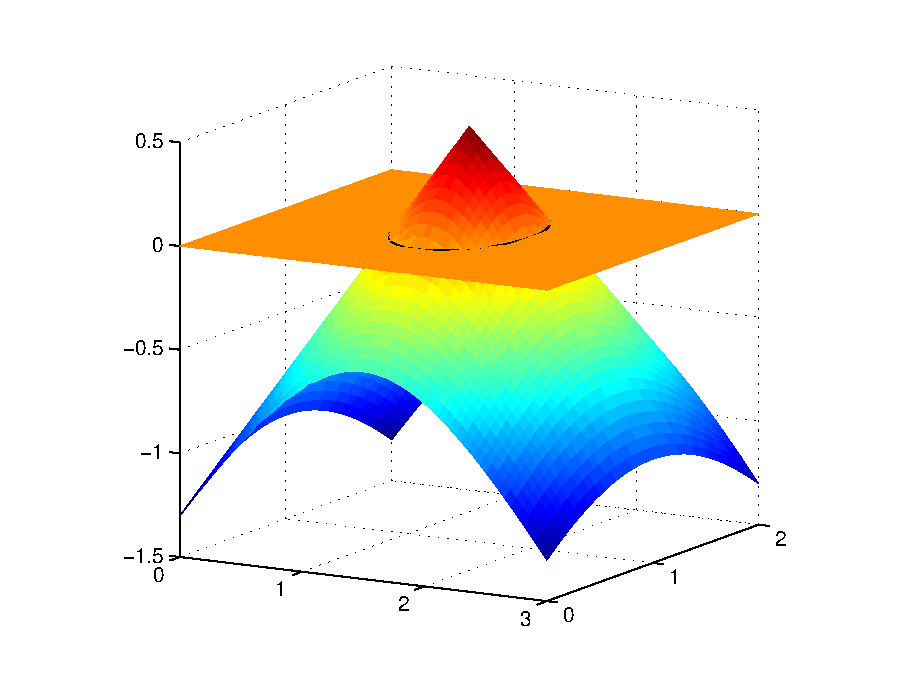
\includegraphics[width=\linewidth]{level_set_circle_func_050.eps}
		} &
		\subfloat[]{
			\label{fig:level_set_circle_domain_1}
			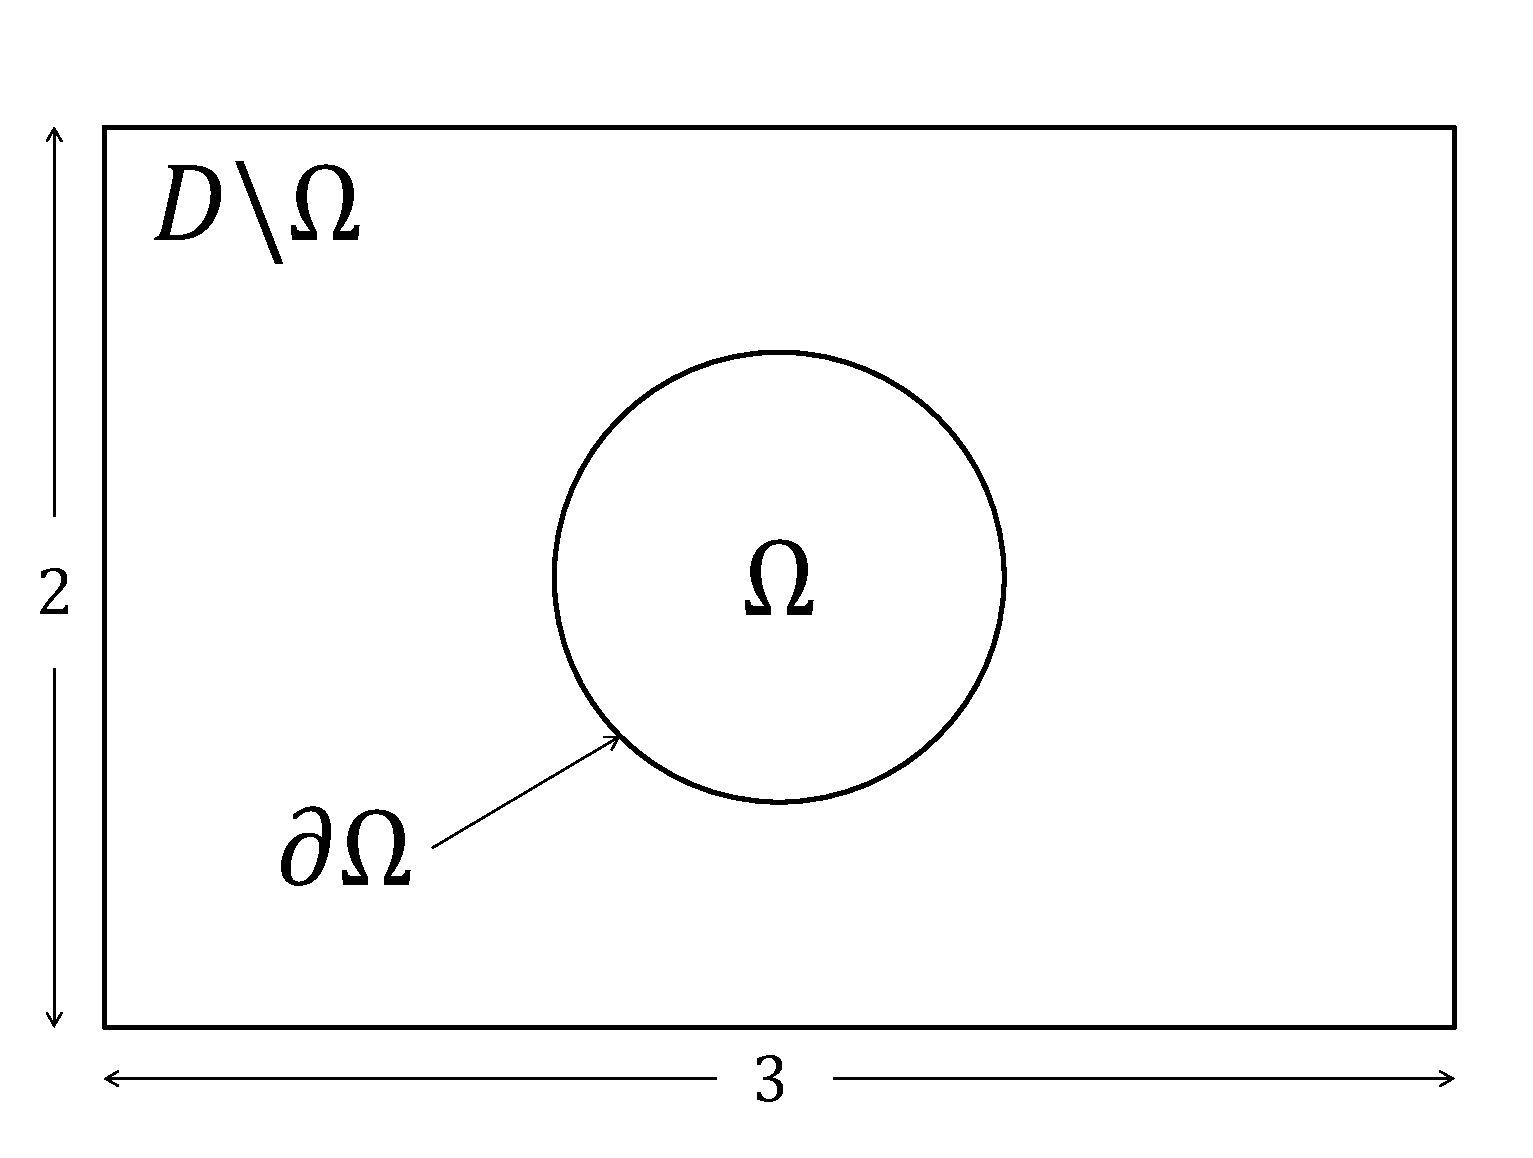
\includegraphics[width=\linewidth]{level_set_circle_domain_050.eps}
		}
	\end{tabularx}
	\caption{The zero level set isolevel of the level set function, $\partial \Omega = \Gamma_{\phi=0}$, in \ref{fig:level_set_circle_func_1} divides the fixed mesh grid into different phase regions in \ref{fig:level_set_circle_domain_1}, where each phase may represent a different material or a different physics.}
	\label{fig:level_set_circle_description}
\end{figure}

To illustrate the differences in the geometry representation between the density and level set methods, consider the ``solid-void'' structural optimization problem presented in Figure \ref{fig:structural_compliance_setup}, where the objective is to minimize the structural compliance by changing the material layout, subject to a maximum volume fraction of 0.5 for the solid phase. The results for both the density and level set approaches are shown in Figure \ref{fig:structural_compliance_comparison}. Notice both designs generate similar truss-like geometries. Figure \ref{fig:structural_compliance_comparison_SIMP} shows how the density method represents the interface between the solid and void materials as intermediate ``grey'' densities, while the level set method in Figure \ref{fig:structural_compliance_comparison_XFEM} describes the geometry by cutting the elements.
%
\begin{figure}[H]
	\centering
	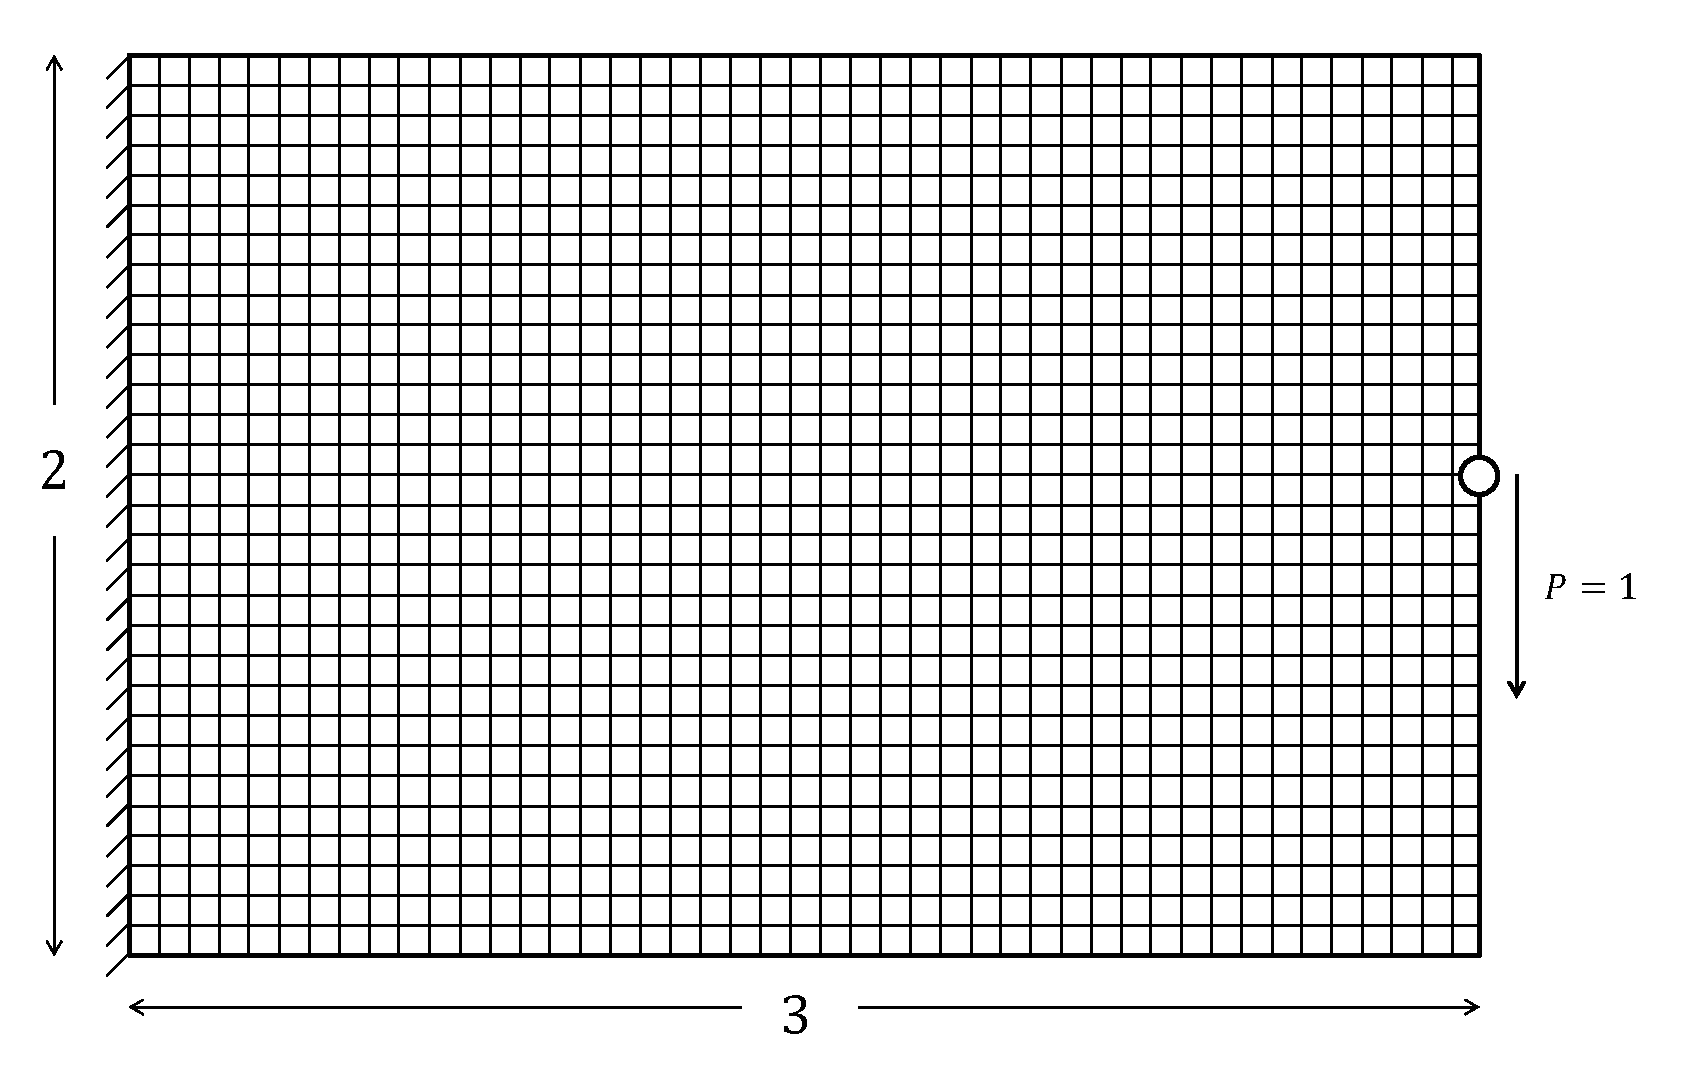
\includegraphics[scale=0.4]{structural_compliance_setup.eps}
	\caption{Setup of a structural topology optimization problem. A mesh of size $3L \times 2L$, with $45 \times 30$ quadrilateral linear elements is anchored to the wall on its left side, and subject to a point load on its right side.}
	\label{fig:structural_compliance_setup}
\end{figure}
%
\begin{figure}[H]
	\centering
	\begin{tabularx}{0.75\linewidth}{X}
		\subfloat[Density method.]{
			\label{fig:structural_compliance_comparison_SIMP}
			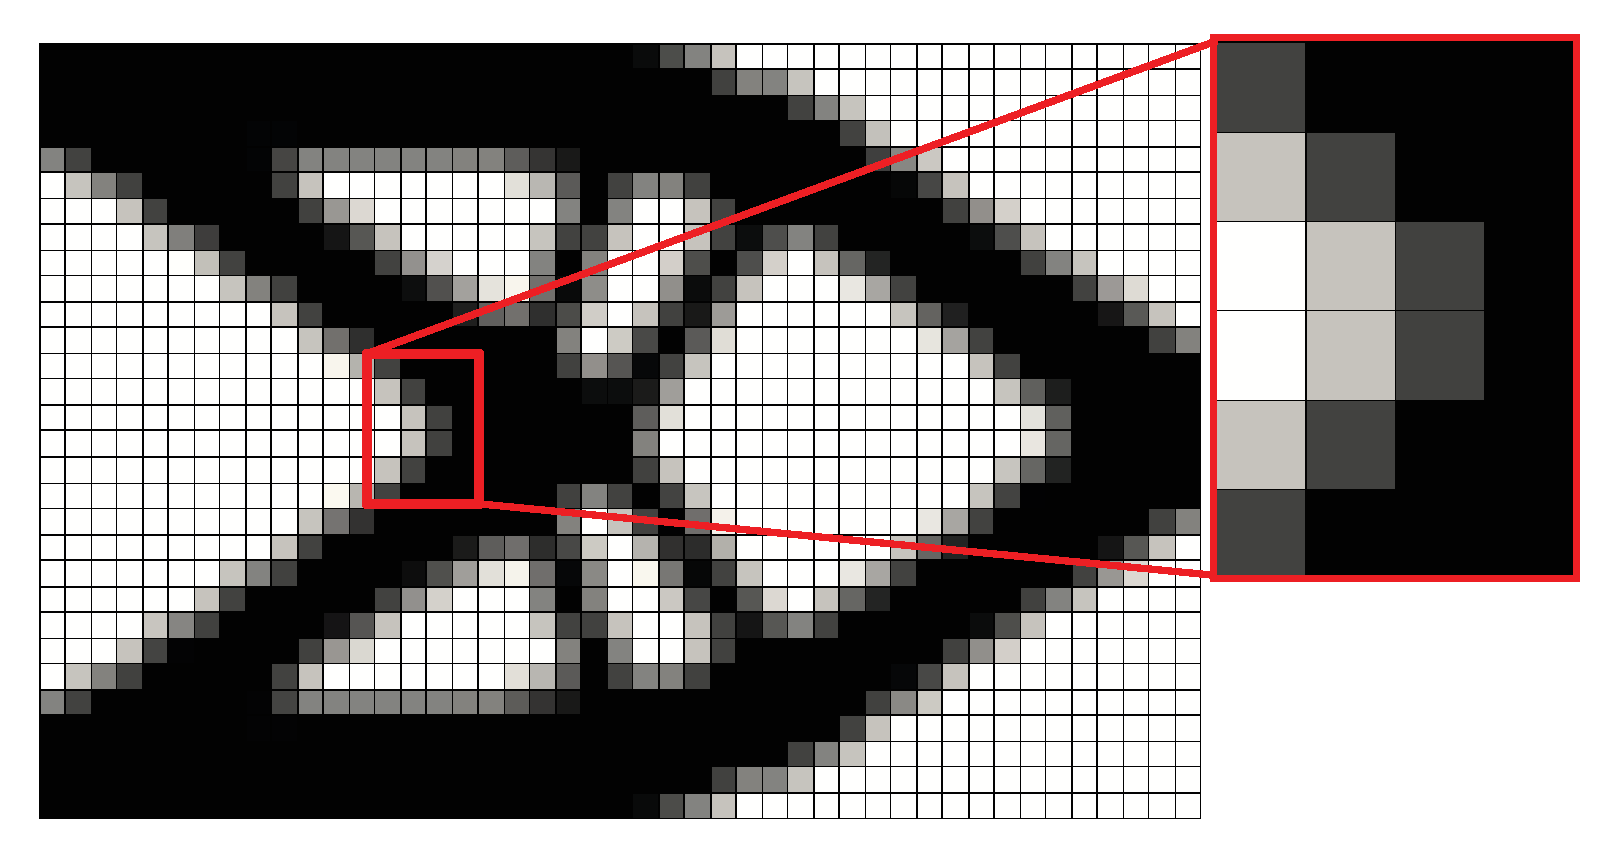
\includegraphics[width=\linewidth]{structural_compliance_comparison_SIMP.eps}
		} \\
		\subfloat[Level set method.]{
			\label{fig:structural_compliance_comparison_XFEM}
			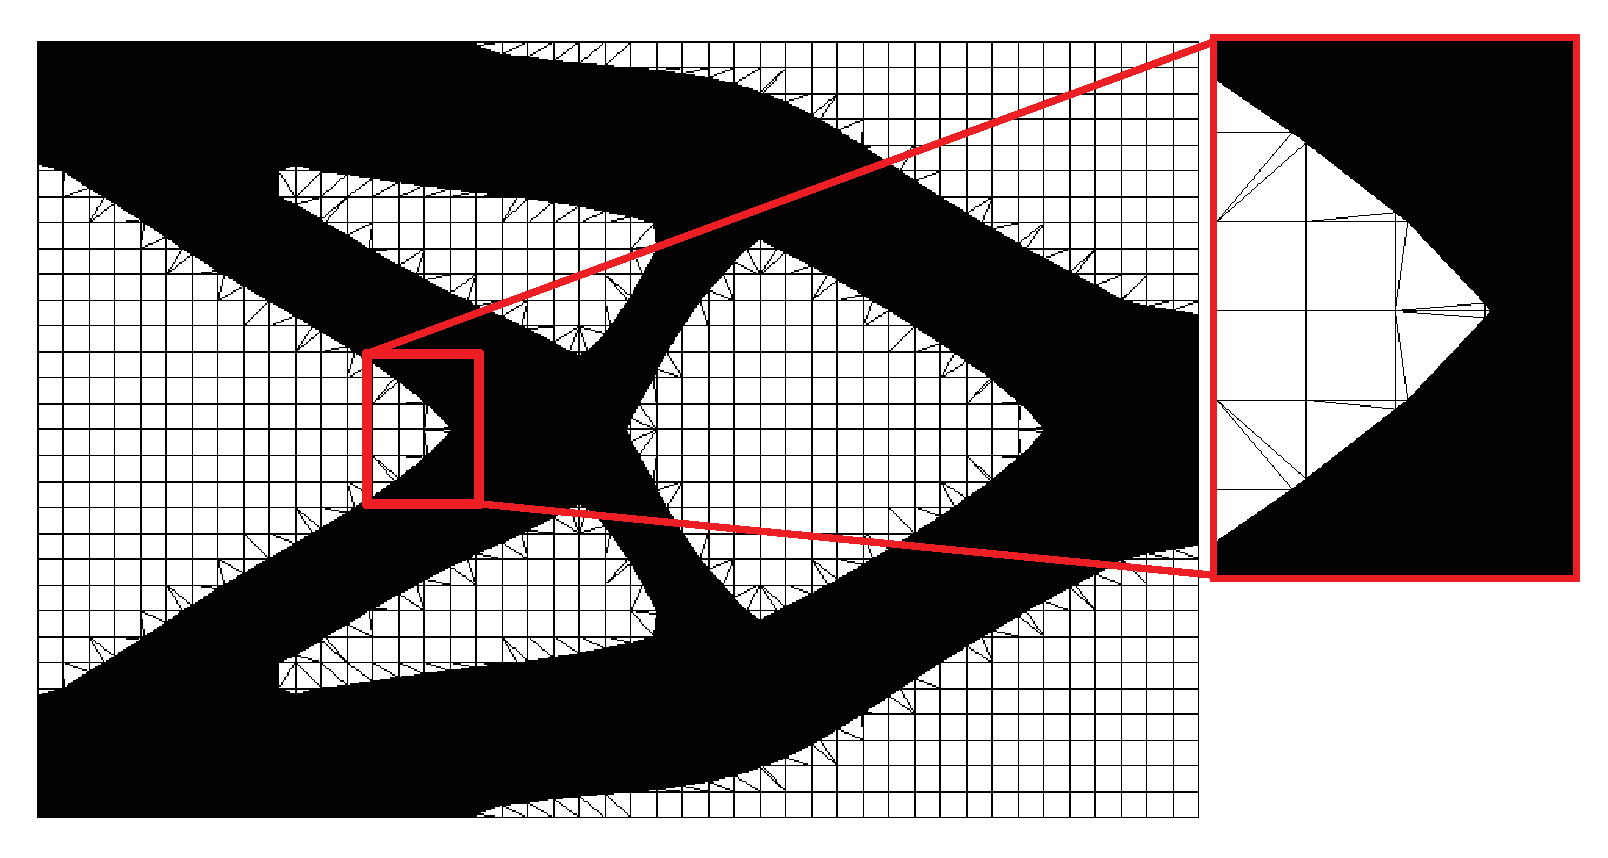
\includegraphics[width=\linewidth]{structural_compliance_comparison_XFEM.eps}
		}
	\end{tabularx}
	\caption{Comparison of the geometry representation of the density and level set methods for a ``solid-void'' structural topology optimization problem.}
	\label{fig:structural_compliance_comparison}
\end{figure}

In the level set method, the material properties of the structural finite elements are interpolated between the void and solid phases, proportional to the volumes of the individual phases. This approach is called Ersatz material interpolation and it is very similar to the interpolation used in density methods. Therefore, it leads to similar issues with regard to enforcing boundary conditions and predicting the physical response along the boundary. The process is illustrated in Figure \ref{fig:ersatz_interpolation}.
%
\begin{figure}[H]
	\centering
	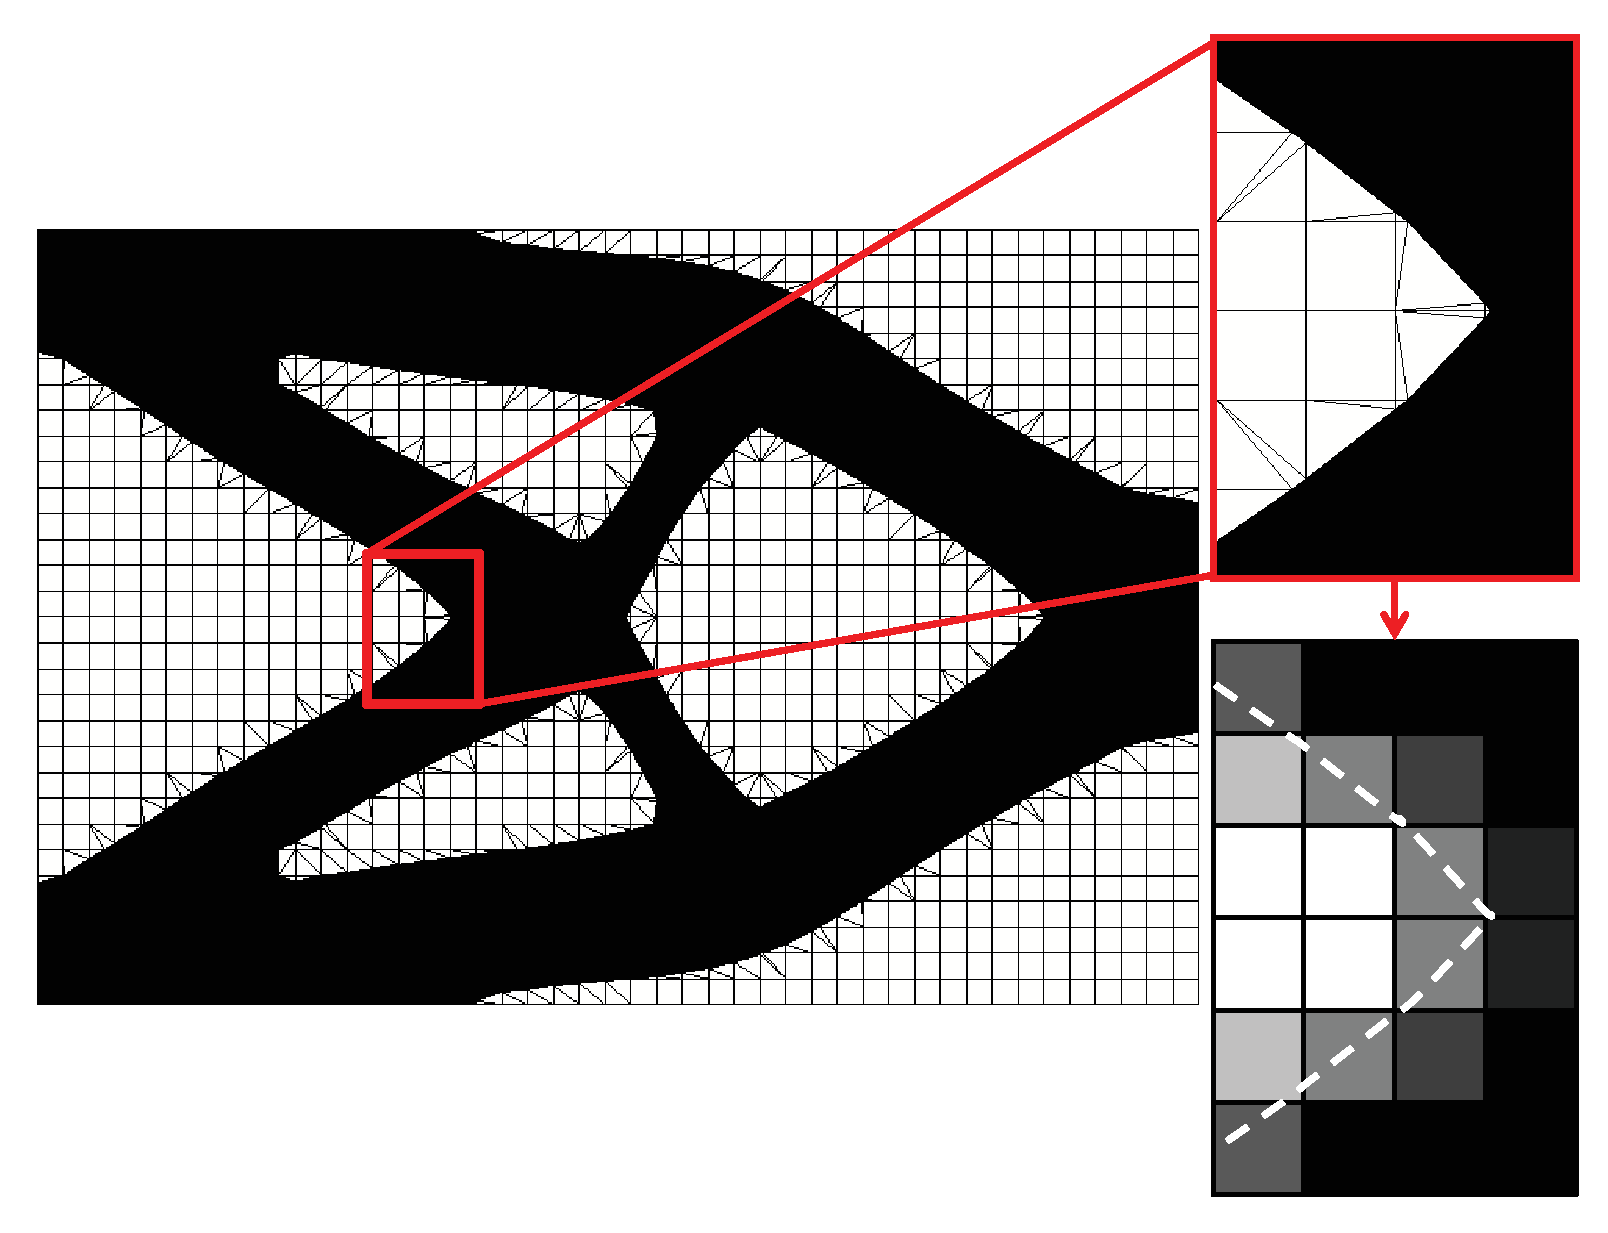
\includegraphics[scale=0.4]{ersatz_interpolation.eps}
	\caption{In an Ersatz material interpolation approach, the material properties of each finite element are interpolated proportional to the volumes of the solid and void phases.}
	\label{fig:ersatz_interpolation}
\end{figure}

An alternative to the Ersatz interpolation is to repeatedly generate new meshes that align with the geometry of the zero level set isolevel, as shown in Figure \ref{fig:remeshing_interpolation}. However, generating an entirely new body fitted
mesh typically suffers from robustness and efficiency, particularly for three dimensional problems. It was also shown by \citep{SMR:00} and \citep{WKG:06} that this method affects the convergence of the optimization process.
%
\begin{figure}[H]
	\centering
	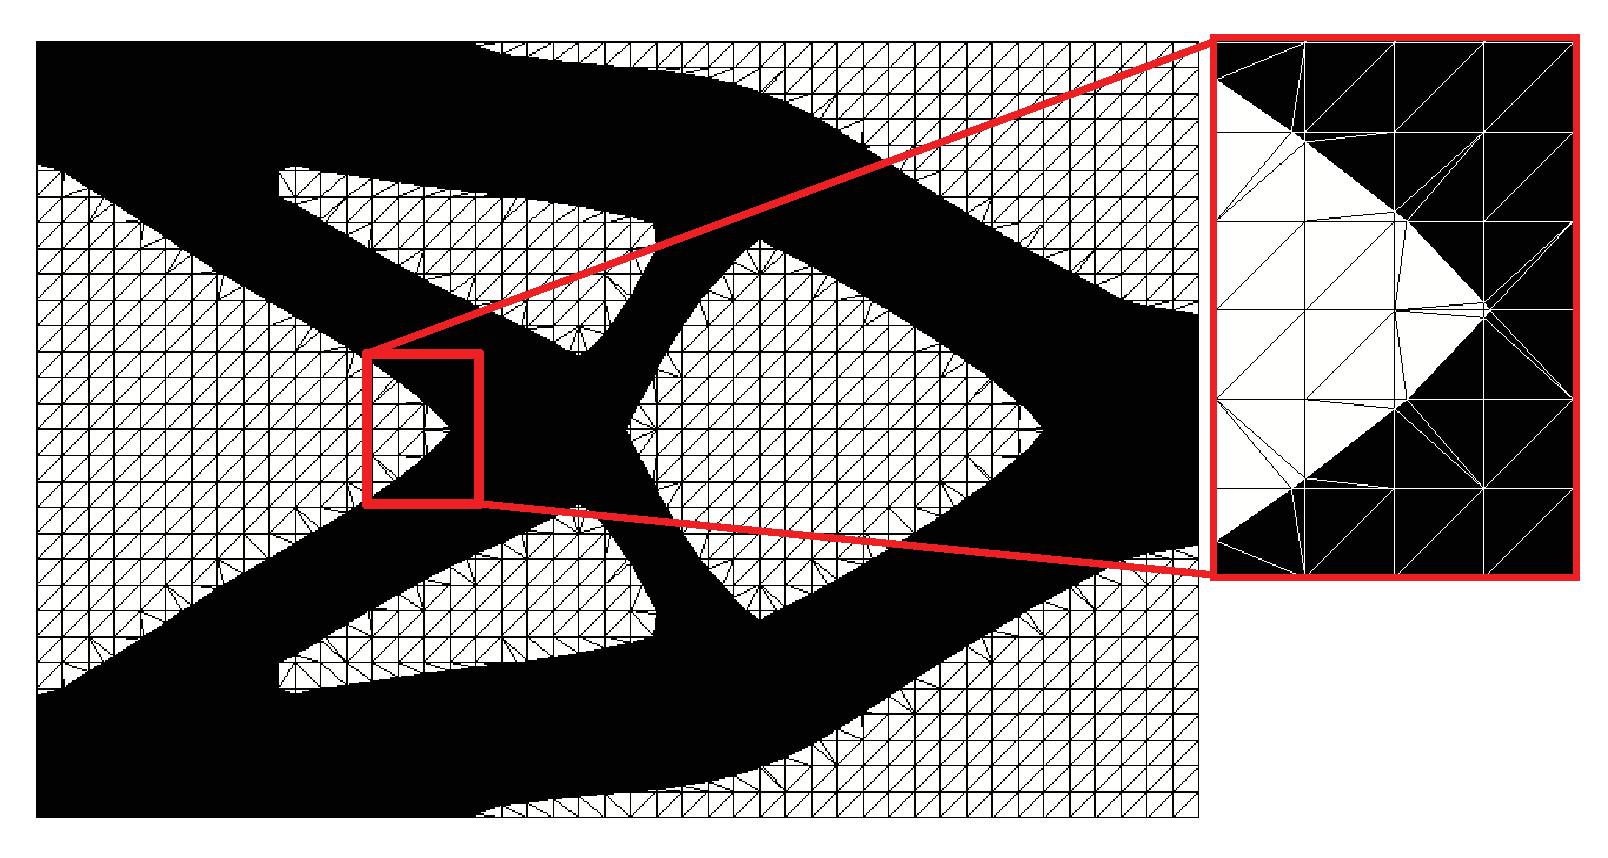
\includegraphics[scale=0.4]{structural_compliance_comparison_remeshing.eps}
	\caption{Remeshing the design domain such that elements align with the zero level set isolevel is an alternative to the Ersatz material interpolation approach.}
	\label{fig:remeshing_interpolation}
\end{figure}

Another approach is used by the XFEM (Section \ref{sec:intro_xfem}). The XFEM is an immersed boundary technique that works on fixed grids, and decomposes the cut elements into subdomains and interfaces that it uses for integration, as shown in Figure \ref{fig:XFEM_interpolation}.
%
\begin{figure}[H]
	\centering
	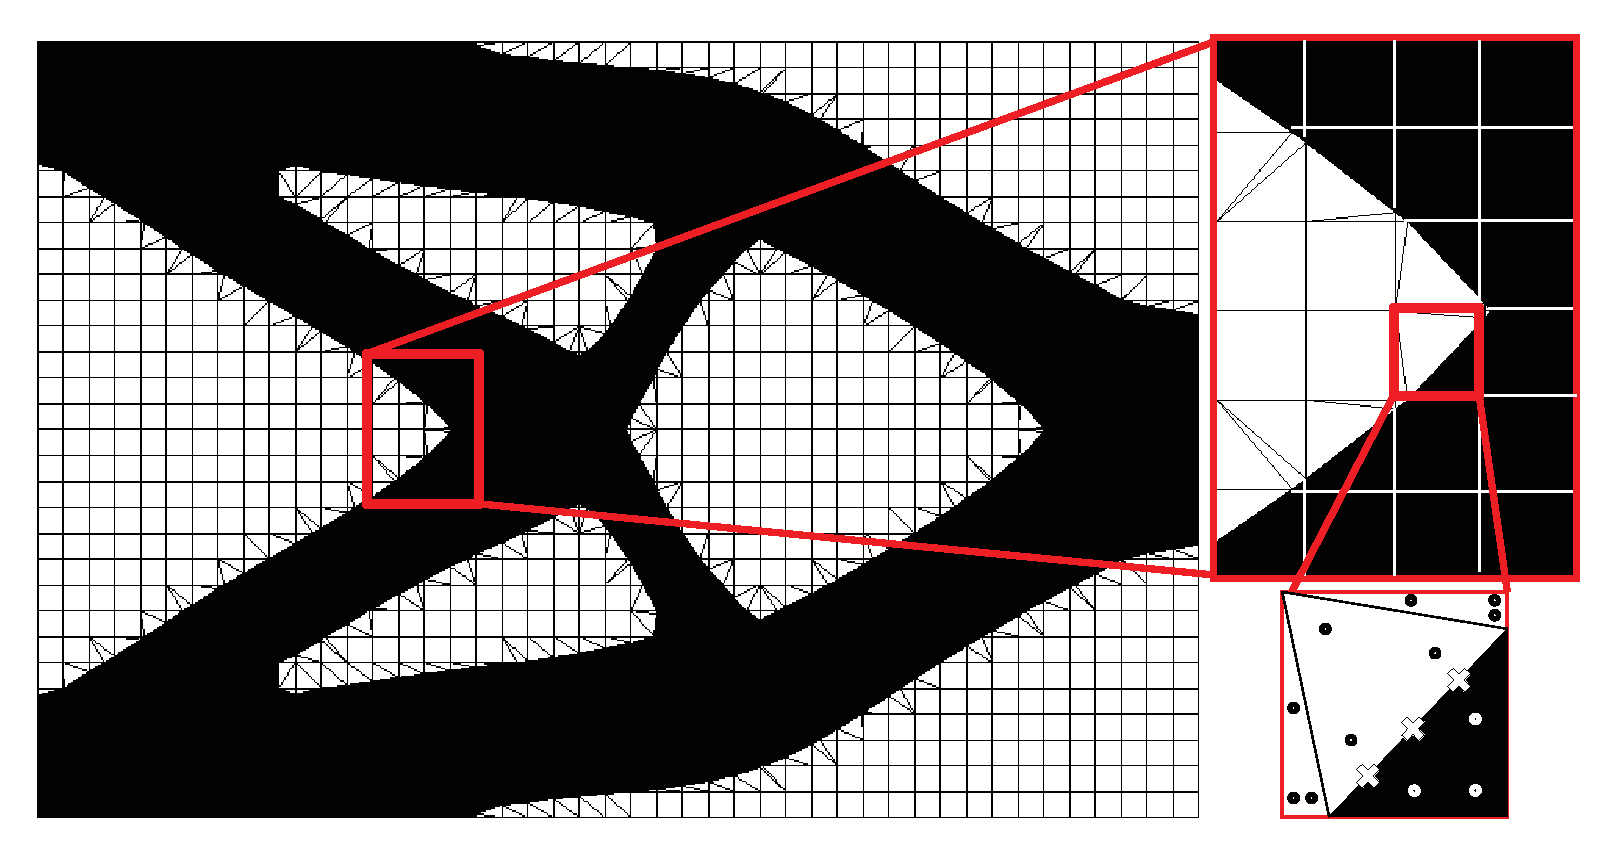
\includegraphics[scale=0.4]{XFEM_interpolation.eps}
	\caption{In the XFEM, the elements cut by the zero level set isolevel are divided into subdomains and interfaces for integration. Circles represent the abscissae for the subdomains, while crosses represent the abscissae for the interface integration.}
	\label{fig:XFEM_interpolation}
\end{figure}

The XFEM enriches the finite element solution space allowing for discontinuities (see Sections \ref{sec:discretization} and \ref{sec:computational-considerations} for details). In this thesis proposal, we will use a Heaviside enrichment strategy, which allows for solution fields with discontinuities $C^{-1}$.

As the topology of the level set function changes, it will occur that a phase subdomain is small enough to cause numerical instabilities in the system, and not lead to convergence. Several approaches have been studied in the literature to try and ameliorate this issue. \citep{LMD+:13} introduced a preconditioner that scales the solution space proportional to the areas of the subdomains. \citep{BH:12,SW:14,SRG+:14} used a ghost penalty formulation to smooth the gradients of the solution at the facets of the cut elements. Both approaches presented favorable results for two dimensional diffusion and incompressible Navier-Stokes flow problems.

Perimeter or curvature measures can be computed at the level set interface using the XFEM. These measures can be introduced into the optimization problem in order to provide a global shape control feature, and prevent the appearance of small floating particles \citep{MM:13}.

This thesis proposal will analyze the characteristics of the proposed LSM-XFEM method as follows:

\begin{enumerate}
	\item \citep{MM:13} studied the XFEM decomposition of the cut elements into subdomains, and the application of multiple enrichment levels in two dimensional problems. Our first hypothesis is that the same approach used by \citep{MM:13} can be extended to three dimensions. Section \ref{sec:a_complete_methodology_for_the_implementation_of_XFEM_inclusive_models} studies the algorithmic details of the approach, and the robustness of the method to describe complex three dimensional geometries using the level set method.

	\item The next question is whether the method can accurately describe the physics at the phase interface without extensive mesh refinement. If so, does it provide an advantage over the interface description provided by the density methods? There are several approaches to approximate the solution at the interface of the level set field, as described in Section \ref{sec:intro_xfem}. We will study the application of stabilized Lagrange multipliers in Section \ref{sec:density_and_level_set_XFEM_schemes_for_topology_optimization_of_3D_structures}, and of the Nitsche method in Section \ref{sec:level_set_XFEM_topology_optimization_of_3D_navier_stokes_and_scalar_transport_problems}.

	\item If the framework can describe complex geometries generated by a level set field, as well as accurately represent the physics at the phase interface, how does it fare overall against density approaches? Section \ref{sec:density_and_level_set_XFEM_schemes_for_topology_optimization_of_3D_structures} applies the framework to three dimensional structural problems, and provides a comprehensive comparison against density methods. The objective is to study convergence rates of the optimization problems, shape control of the optimized geometries, postprocessing capabilities of the methods to generate manufacturable designs, and the effects of providing different initial designs to the optimization process. The hypothesis is that the framework provides a better description of the geometry and material distribution than density methods, and therefore requires coarser meshes which leads to faster computations. Furthermore, it provides the capability to extract surface meshes directly from the level set function and manufacture the designs using three dimensional printing. This feature would be promising for rapid-prototyping.

	\item  In section \ref{sec:preconditioner}, we will expand the scaling preconditioning scheme to structural problems. The preconditioner was previously studied for two dimensional heat conduction problems. The scaling should ameliorate the effects that small intersection regions cause to the solution. In section \ref{sec:level_set_XFEM_topology_optimization_of_3D_navier_stokes_and_scalar_transport_problems}, we will study an alternate approach, the face-oriented ghost-penalty, and its effects on incompressible Navier-Stokes flows. This penalty formulation has been studied in the literature for diffusion and incompressible Navier-Stokes problems, and our hypothesis is that it can be applied in our optimization framework to ensure convergence for three dimensional problems.

	\item Once we can ensure convergence of the solution, the framework should be able to solve a broad range of design engineering problems. In this thesis proposal, we will study structural, incompressible Navier-Stokes flow, and scalar transport problems. These physics will help understand the characteristics, and the capability of the method to be applied to real-world engineering problems. Structural problems are studied in Section \ref{sec:density_and_level_set_XFEM_schemes_for_topology_optimization_of_3D_structures}. Incompressible Navier-Stokes and scalar transport problems are studied in \ref{sec:level_set_XFEM_topology_optimization_of_3D_navier_stokes_and_scalar_transport_problems}.

	\item Controlling the shape of the optimized geometry is important in manufacturing. The effects of using a smoothing filter for the level set field (see Section \ref{sec:intro_level_set_method}) will be studied in Section \ref{sec:feature-size-control}. This filter will also be compared against the density filter (see Section \ref{sec:smoothing_filter}) as a way of controlling the minimum feature size. Regularization techniques applied to the level set interface, such as measuring the curvature and perimeter, may cause different optimized geometries to emerge. The use of these measures and its effects on the finalized design will be studied in Section \ref{sec:topology_optimization_approaches_for_the_curvature_minimization_of_level_set_isocontours}.
\end{enumerate}

The studies proposed above will help us understand the characteristics and capabilities of the framework. The final step is to use this knowledge to study the method in the context of a real-world problem that requires the modeling of a three dimensional incompressible Navier-Stokes flow with a scalar transport field in Section \ref{sec:modeling_of_multiple_scalar_transport_fields_for_an_atomic_layer_deposition_machine}.

The specific objectives of this thesis proposal are then:
\begin{inparaenum}[(i)]
	\item To generate a robust LSM-XFEM topology optimization scheme;
	\item To compare the LSM-XFEM optimization scheme with traditional homogenization methods, such as SIMP, and study the advantages and disadvantages of our formulation;
	\item and to explore the characteristics of the methodology through cases studies in selected applications.
\end{inparaenum}

The layout of this thesis proposal is as follows: Section \ref{sec:introduction} presented the motivation and goals of the study, Section \ref{sec:background} presents an overview of the concepts required to understand this work, Section \ref{sec:a_complete_methodology_for_the_implementation_of_XFEM_inclusive_models} presents the algorithm to implement an XFEM framework in software, Section \ref{sec:density_and_level_set_XFEM_schemes_for_topology_optimization_of_3D_structures} presents the application of the methodology in structural problems, and compares the results to density approaches, Section \ref{sec:level_set_XFEM_topology_optimization_of_3D_navier_stokes_and_scalar_transport_problems} presents the application of the method to incompressible Navier-Stokes flows and scalar transport problems, Section \ref{sec:topology_optimization_approaches_for_the_curvature_minimization_of_level_set_isocontours} studies regularization techniques to improve the manufacturing of the design, Section \ref{sec:modeling_of_multiple_scalar_transport_fields_for_an_atomic_layer_deposition_machine} uses the methodology for a real-world design engineering problem. Finally, Sections \ref{sec:remaining_work} and \ref{sec:main_conclusions} show the remaining work and conclusions of this thesis proposal.

% -----------------------------------------------------------------------------

\chapter{Background}
\label{sec:background}

This chapter presents a brief overview on topology optimization, the level set method, and finite element methods. The information presented in this chapter is sufficient such that the reader can understand the framework in which the thesis is developed, but it is not comprehensive. References are provided for the reader who wishes to see more details on the topics.

% -----------------------------------------------------------------------------

\section{Optimization}
\label{sec:optimization}

An optimization problem is a problem in which you seek to find the best solution from the set of all feasible solutions. There are two categories of optimization problems, and their classification depends on whether the problem variables are continuous or discrete. In this work, we will focus on optimization problems with continuous variables. An optimization problem with discrete variables is known as a combinatorial optimization problem, and the reader is directed to \citep{NW:88} for a review.

The standard form for an optimization problem with continuous variables is:
%
\begin{equation}
\label{eq:optimization_standard_form}
	\begin{aligned}
		&\min_{\mathbf{s}} \mathcal{F}(\mathbf{s}, \mathbf{u}(\mathbf{s})), \\
		&\text{s.t.\,}
		\begin{cases}
			\mathbf{s}, & \text{subject to design constraints}  \ \mathcal{G}_j \leq 0 \text{,}\\
			\mathbf{u}, & \text{solves} \ W= 0 \ \text{for a given $\mathbf{s}$,}
		\end{cases}
	\end{aligned}
\end{equation}
%
where the goal is to minimize some objective functional $\mathcal{F}$ with respect to the vector of design variables $\mathbf{s}$. The design variables are subject to the $j$-th design constraint $\mathcal{G}_j$, which are enforced as an inequality problem. In general, the objective and constraints depend on the optimization variables, $\mathbf{s}$, and the state variables, $\mathbf{u}$. These state variables, $\mathbf{u}$, satisfy the weak form of the equilibrium equation $W$, which is enforced as an equality constraint. By convention, Equation \ref{eq:optimization_standard_form} defines a minimization problem. Maximization problems are handled by placing a negative sign on the objective functional $\mathcal{F}$.

% -----------------------------------------------------------------------------
% Optimization algorithms

There are several optimization algorithms available to update the design variables. For structural optimization problems with non-trivial and multiple constraints, the Method of Moving Asymptotes (MMA) \citep{Svanberg:87}, and its globally convergent counterpart, the Globally Convergent Method of Moving Asymptotes (GCMMA) \citep{Svanberg:02} have become the algorithms of choice. The work of this document will focus on the GCMMA algorithm. For a reference on more advanced mathematical tools, such as thr Sequential Quadratic Programming (SQP), the Sparse Nonlinear OPTimizer (SNOPT) \citep{GMS:02}, or the Interior Point OPTimizer \citep{WBL:06}, the reader is referred to the work of \citep{SM:13}.

% -----------------------------------------------------------------------------
% Design sensititivies

Gradients of the objective functional and design constraints with respect to the design variables are required by the mathematical algorithms specified above. The sensitivities for the optimization problems presented in this document will be computed using the adjoint method \citep{GP:08,YSL:02}.

In the following sections, we will delve into the approaches available to solve the optimization problem.

% -----------------------------------------------------------------------------

\section{Topology optimization}
\label{sec:intro_topology_optimization}

Topology optimization is a type of optimization problem in which you seek the optimal geometry and/or material layout of a body within a given design domain $D$. For example, mathematically we can formulate the following generic topology optimization problem: 
%
\begin{equation}
\label{eq:topology_optimization_generic}
		\min_{\mathbf{s}} \int_{\Omega} f \left( \mathbf{s(\mathbf{x})} \right) d{\Omega}
\end{equation}
%
which, analogous to Equation \ref{eq:optimization_standard_form} is subject to design constraints and equilibrium equations. The goal of the optimization problem is to minimize some objective functional $\int_{\Omega} f \left( \mathbf{s(\mathbf{x})} \right) d{\Omega}$ over the design domain with respect to the design variables $\mathbf{s(\mathbf{x})}$, where $\Omega$ represents the shape of the design. The optimization problem will set the design variables as ``on'' or ``off'' in order to minimize the design objective, while satisfying the design constraints. We can represent a design variable at a point $i$ as ``on'' by setting $s_{i}=1.0$, and ``off'' by $s_{i}=0.0$. A quick example is described in Figures \ref{fig:structural_compliance_setup} and \ref{fig:structural_compliance_example}. Figure \ref{fig:structural_compliance_setup} shows the setup for a topology optimization problem with an objective of minimal compliance and subject to a maximum volume fraction of $0.5$ for the solid phase. Figure \ref{fig:structural_compliance_example} shows the changes in the design, where the design variables at the elements are represented as ``on'' (black) or ``off'' (white) or in-between (grey).
%
\begin{figure}
	\centering
	\begin{tabularx}{\linewidth}{XX}
		\subfloat[Step 0.]{
			\label{fig:structural_compliance_0}
			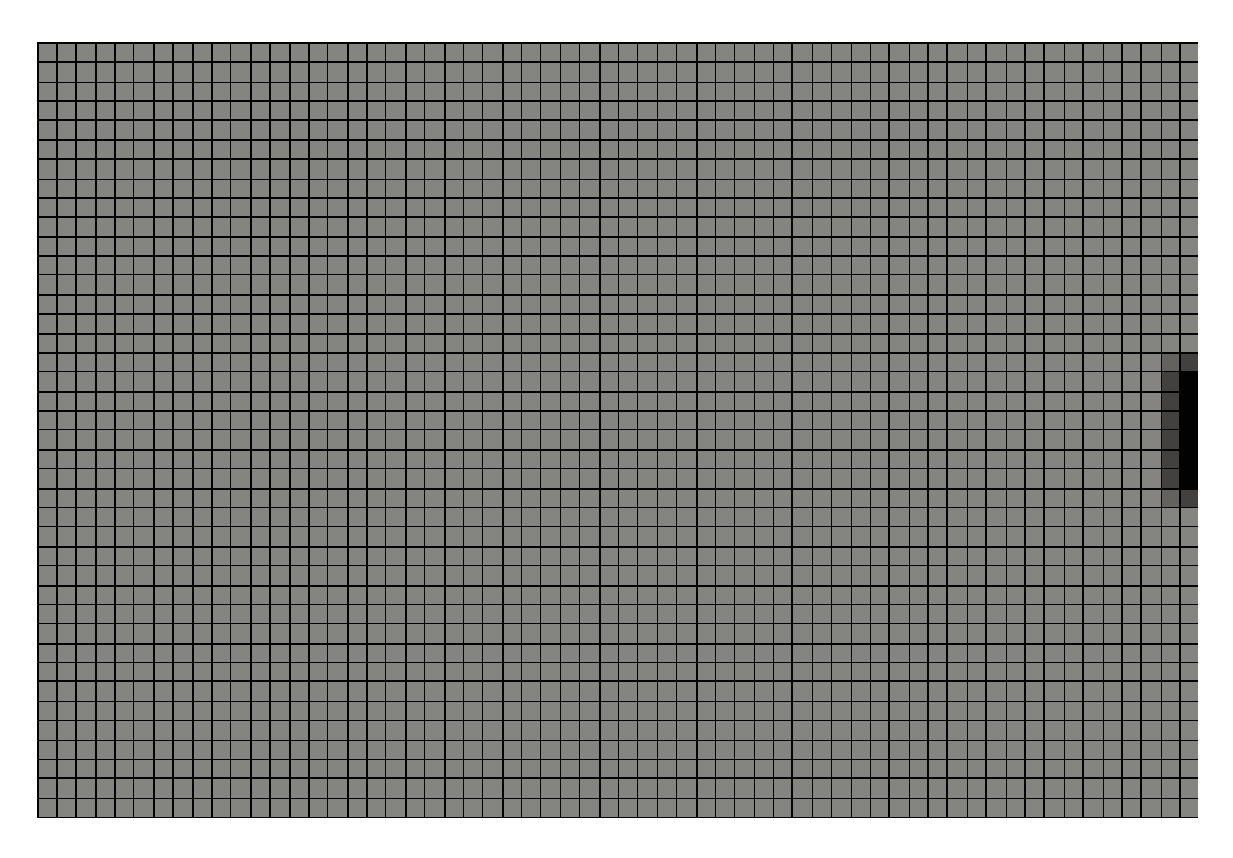
\includegraphics[width=\linewidth]{structural_compliance_0.eps}
		} &
		\subfloat[Step 5.]{
			\label{fig:structural_compliance_5}
			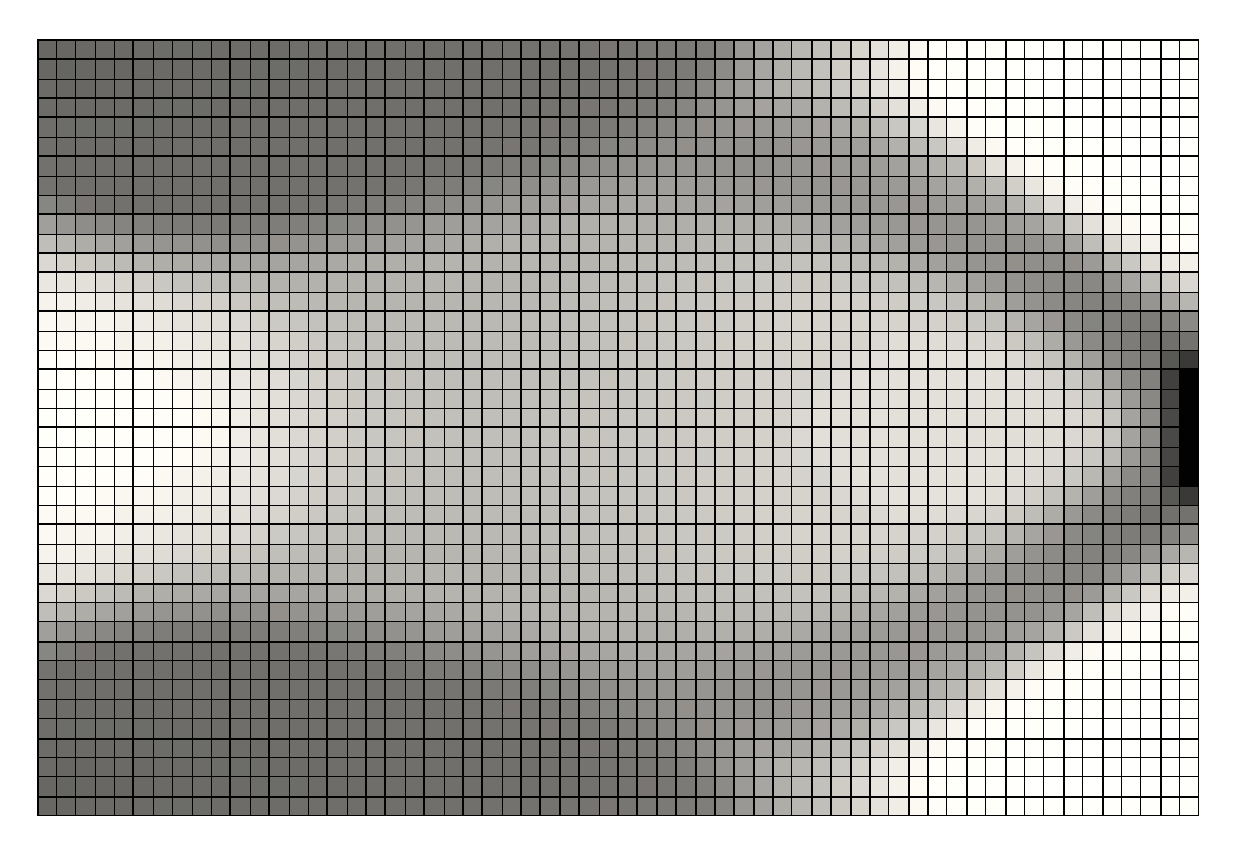
\includegraphics[width=\linewidth]{structural_compliance_5.eps}
		} \\
		\subfloat[Step 10.]{
			\label{fig:structural_compliance_10}
			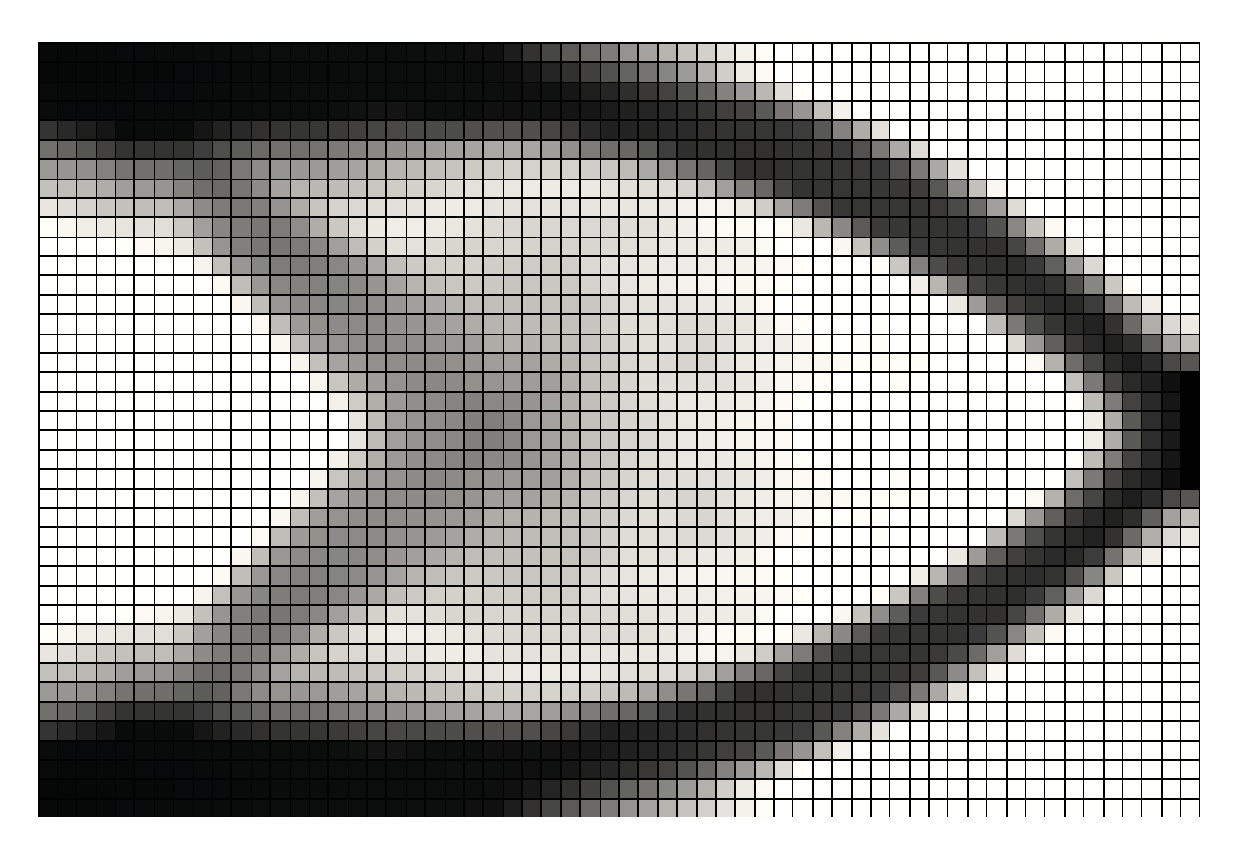
\includegraphics[width=\linewidth]{structural_compliance_10.eps}
		} &
		\subfloat[Step 15.]{
			\label{fig:structural_compliance_15}
			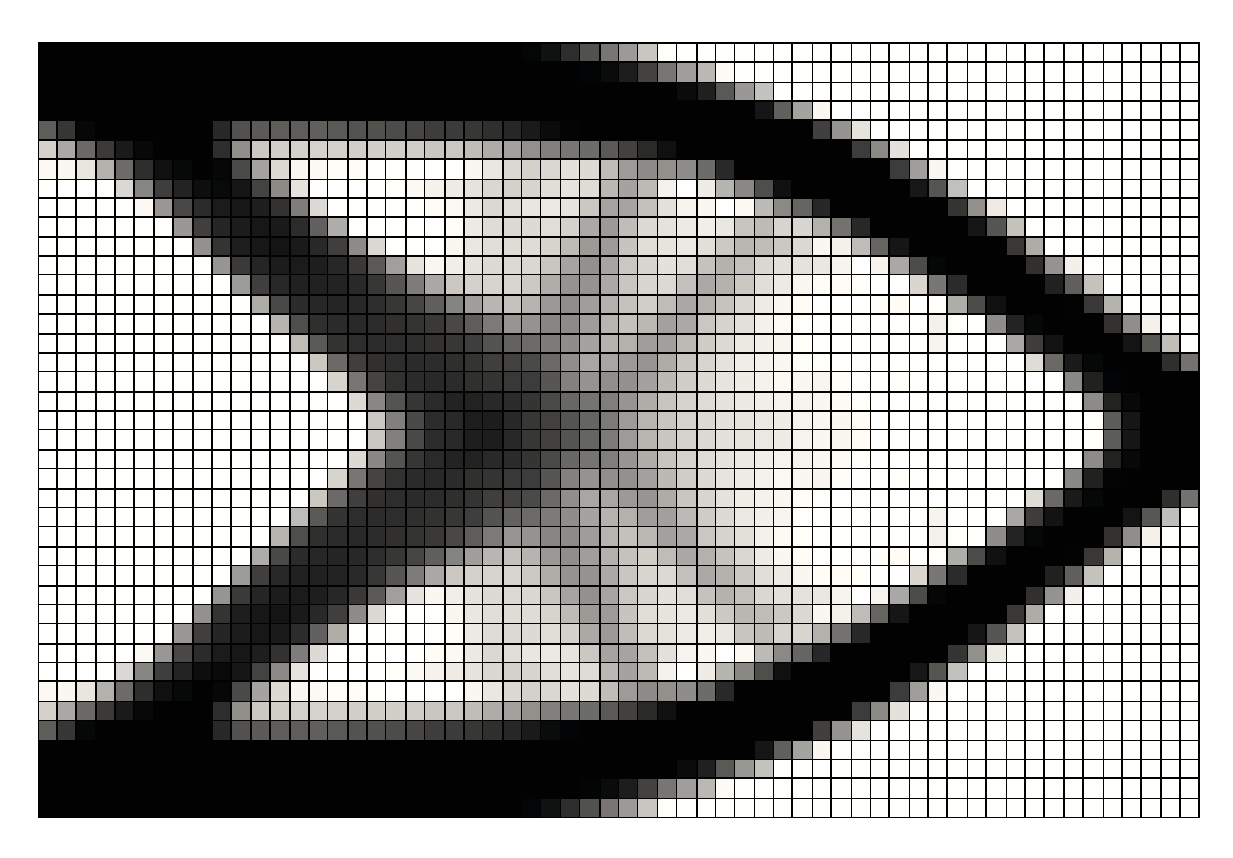
\includegraphics[width=\linewidth]{structural_compliance_15.eps}
		} \\
		\subfloat[Step 25.]{
			\label{fig:structural_compliance_25}
			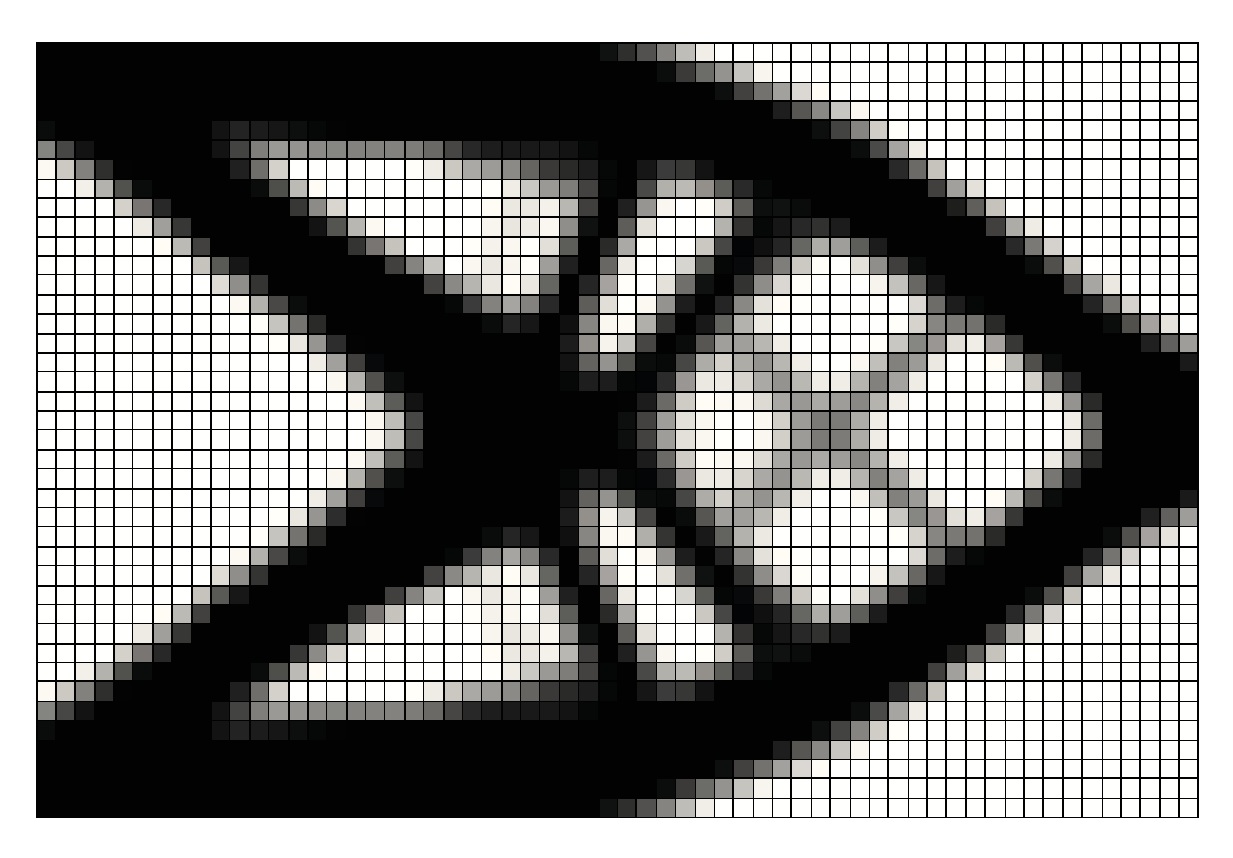
\includegraphics[width=\linewidth]{structural_compliance_25.eps}
		} &
		\subfloat[Step 50.]{
			\label{fig:structural_compliance_50}
			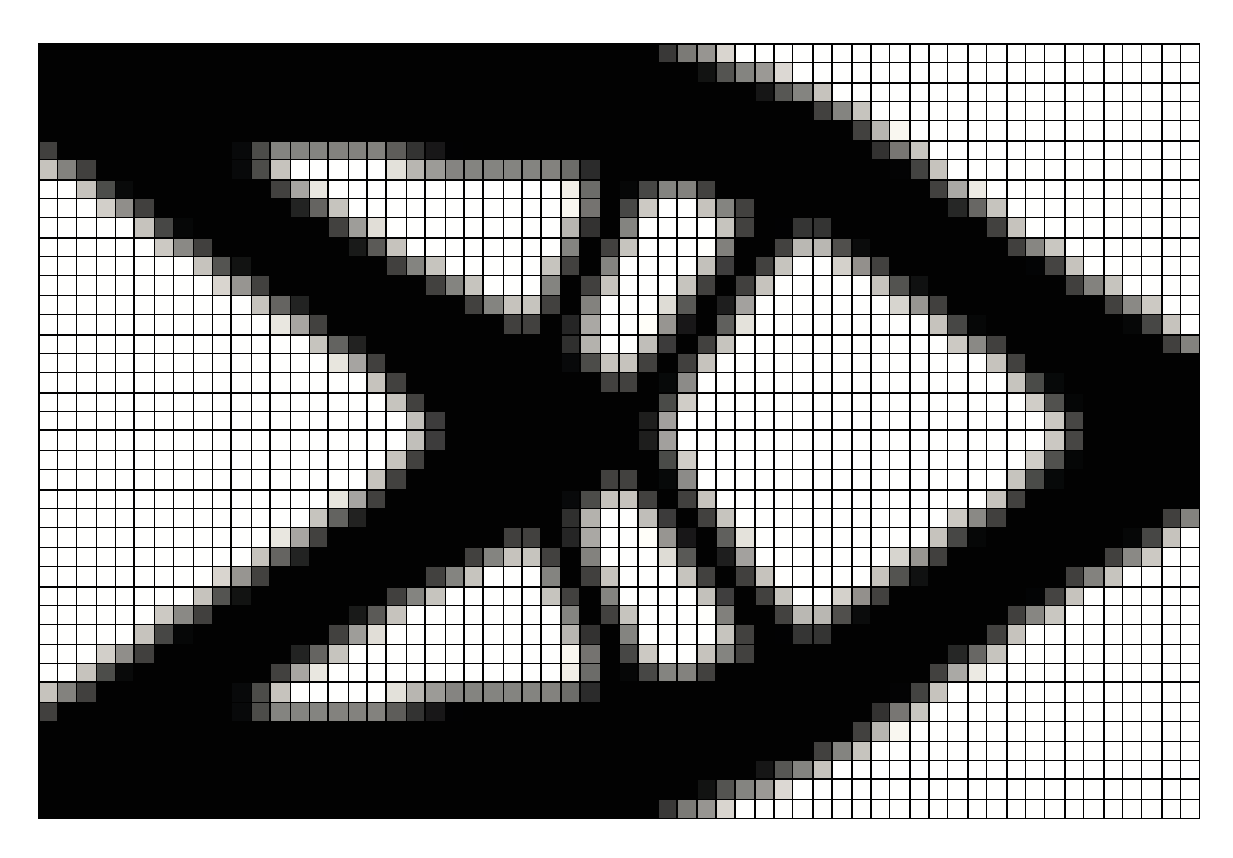
\includegraphics[width=\linewidth]{structural_compliance_50.eps}
		} \\
	\end{tabularx}
	\caption{Progression of the optimization process. Objective is to minimize compliance subject to a maximum volume fraction of 0.5 for the solid phase.}
	\label{fig:structural_compliance_example}
\end{figure}

Topology optimization provides the ability to create designs that are not always intuitive, or to improve on existing designs. Topology optimization methods were initially developed to create conceptual designs in the early stage of the design process \citep{BS:03,Rozvany:09}. It is interesting to note that the earliest recorded paper on topology optimization dates back to 1904, with the work of Australian inventor Michell in the derivation of optimality criteria for least-weight layout of trusses \citep{Michell:04}. And while topology optimization focused for decades on structural design, it has recently found its application in a wide range of physical disciplines \citep{BLO+:05} including acoustics \citep{FAN+:04}, wave propagation \citep{Frenzel:04}, electromagnetics \citep{LGD:09,SHW+:08} and optics \citep{BHF+:04,KOY:05}. For a more detailed review on topology optimization, please refer to \citep{BS:03,EO:01}.

% \footnote{\label{fn:topopt_app}
% At this point, the author recommends you take out your iPhone and iPad and download the best (and ahem... only) structural topology optimization application in the market, TopOpt, from the DTU Mechanical Engineering department. Use this as an exercise to reinforce the concepts explained in this paragraph. Start the application and define a structural problem adding boundary conditions and loads. Before you start the optimization process, try and think of what a good design would be for the problem at hand. Do this for several problems, and compare your intuition to the results of the optimization application. You may realize how helpful topology optimization can be for creating structures with the optimal design.}

% -----------------------------------------------------------------------------
% \subsection{Structural topology optimization}

Structural topology optimization, specifically topology optimization of continuum structures, is in its mathematical nature one of the most challenging optimization problems \citep{BS:03}. However, in 1988, \citep{BK:88} introduced their seminal paper on the homogenization method. In this method, the design domain is assumed to be formed by a material with micro-scale voids, and the topology optimization problem seeks the optimal porosity of the porous medium in order to minimize the objective functional. Due to its effectiveness and simplicity, homogenization-based methods found a lot of applications in structural design, and quickly became the main approach in structural topology optimization \citep{Bendsoe:89}. The homogenization method works by transforming the structural optimization problem into a standard nonlinear program where the design variables are coefficients of the underlying governing equation, and therefore is capable of producing internal holes in the design domain without \textit{a priori} knowledge of them.

% -----------------------------------------------------------------------------

\section{Density topology approaches}
\label{sec:density_topology_approaches}

In 1989, \citet{Bendsoe:89,ZR:91} introduced the most popular of homogenization methods, the ``solid isotropic material with penalization'' (SIMP). In SIMP, the design variables represent the artificial densities, $\rho\left(\mathbf{x}\right)$, of a group of elements in a fixed finite element grid (our design domain $D$) and their material properties are parameterized in terms of a set of material interpolation functions such that intermediate properties are penalized. The typical approach is to assume a value of $\rho=1.0$ represents solid material, while $\rho=0.0$ represents void.

% -----------------------------------------------------------------------------

\subsection{Smoothing filter}
\label{sec:smoothing_filter}

An additional numerical scheme is necessary to smear out numerical instabilities. This is referred to as the filtering method \citep{Sigmund:01a,Sigmund:01b}. For example, in structural topology optimization, the density, rather than being equal to a single variable, can be computed from a linear smoothing filter as follows:

\begin{equation}
	\label{eq:smoothing_filter_SIMP}
	\tilde{\rho}\left(\mathbf{s}\right)=\frac{\sum_{i=1}^{E}w_{i}s_{i}}{\sum_{i=1}^{E}w_{i}}
\end{equation}

with

\begin{equation}
	\label{eq:weight_SIMP}
	w_{i}=\max \left( 0, r_{\rho} - \Vert \mathbf{x}_i - \mathbf{x} \Vert \right)
\end{equation}

where $s_{i}$ is equivalent to an artificial density $\rho$ at a point $\mathbf{x}_{i}$, $\mathbf{x}_{i}$ is the location of the node at which the design variable $i$ is defined, $\tilde{\rho}\left(\mathbf{s}\right)$ is the density at a point $\mathbf{x}$,  $w_{i}$ is the factor of point $\mathbf{x}$ with respect to the design variable $i$, $r_{\rho}$ is the filter radius, and $E$ is the number of elements in the design domain.

The filter in Equation \ref{eq:smoothing_filter_SIMP} prevents the formation of features smaller than $r_{\rho}$, and serves as a minimum feature size control. However, this comes at the cost of forming intermediate densities along the material interface. Methods for smearing out intermediate densities have been proposed by \citep{FJP:05,Sigmund:07,SS:01a}. \citep{GPB:04} proposed a density projection method to reduce the volume occupied by material with intermediate densities. This projection is based on a smoothed Heaviside function and applied to the densities as follows:
%
\begin{equation}
\label{eq:heaviside_density}
		\hat{\rho}\left(\tilde{\rho}\right) = 1-e^{-\beta\tilde{\rho}}+\tilde{\rho}e^{-\beta}
\end{equation}
%
where $\hat{\rho}$ is the projected density, and the parameter $\beta \ge 0$ controls the crispness of the projection. Notice that for $\beta=0$ we recover the original density $\hat{\rho}=\tilde{\rho}$. As we increase $\beta$, more and more intermediate densities are penalized towards the value of 1.0, as shown in Figure \ref{fig:density_heaviside}. Note, however, that if the objective and/or constraints of the optimization problem find the intermediate densities to be benefitial, the optimization algorithm will ignore the effects of this projection scheme. The reader is referred to \citep{GPB:04,GAH:11,Sigmund:07,XCC:10,WLS:11} for more details on projection schemes.
%
\begin{figure}
	\centering
	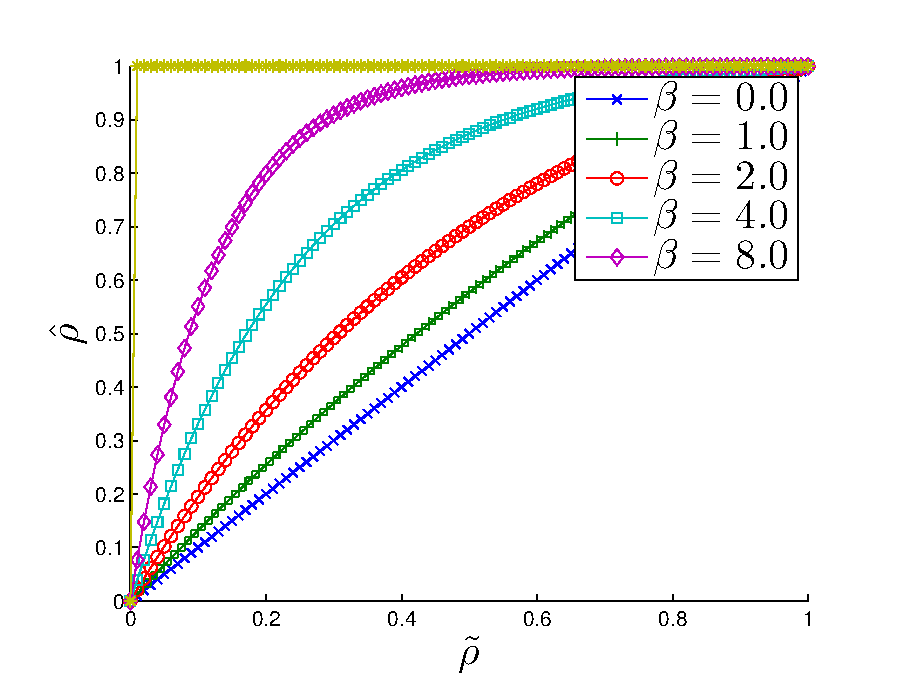
\includegraphics[scale=0.75]{density_heaviside.eps}
	\caption{The density Heaviside projection for various magnitudes of $\beta$.}
	\label{fig:density_heaviside}
\end{figure}
%
In structural topology optimization, it is important to model the relation between density and stiffness. SIMP models the stiffness proportional to the density in the power $p$, where $p > 1$ \citep{BS:99}, in order to guarantee a well-posed optimization problem \citep{BS:99}. The structural stiffness for a ``solid-void'' problem can then be formulated as:
%
\begin{equation}
\label{eq:structural_stiffness}
		E\left(\mathbf{x}\right) = \hat{\rho} ^ p E_{0}
\end{equation}
%
where $E_{0}$ is the initial structural stiffness of the material. Typically, the parameter $p$ is set to 1, and then increased as the optimization progresses \citep{RZS:94}; this is the so-called continuation method \citep{SP:98}. It was shown that if one uses $p > 3$, we recover a black-and-white binary-like material distribution \citep{BS:03}. That is why the density approach has been referred to as a \textit{pixelated} geometric model.

% -----------------------------------------------------------------------------
% Multimaterial SIMP
% \subsection{Multimaterial SIMP}

The SIMP method can be expanded to model a multi-material optimization problem. For example, applying a ``rule of mixture'', we can model a two-phase material in structural topology optimization by modifying Equation \ref{eq:structural_stiffness} as:

\begin{equation}
	\label{eq:two_phase_stiffness}
	E\left(x\right) = \hat{\rho} ^ p E_{A} + \left( 1 - \hat{\rho} ^ p \right) E_{B}
\end{equation}

where $E_{A}$ represents the stiffness of material ``A'', and $E_{B}$ represents the stiffness of material ``B''. Notice that if we model the material phase ``B'' as void, and set $E_{B}=0$ we recover the original equation from \ref{eq:structural_stiffness}. This method uses a single design variable field to model up to two different materials.

For a three-phase or more material optimization problem, we require an extended power law interpolation with multiple design variable fields (i.e. $\mathbf{s}_{1}$, $\mathbf{s}_{2}$, etc.), as shown in \citep{WW:04c,PS:14}. In general, the SIMP method requires $\left( n - 1 \right)$ design variable fields for $n$ distinct material phases \citep{WW:04c}.

% -----------------------------------------------------------------------------

\subsection{Density methods applied to fluid dynamics}
\label{sec:intro_density_fluid_dynamics}

Several applications require finding the optimal geometries of systems to improve the performance of internal and external flows \citep{Maute:14}. Adopting the concept of density methods, \citep{BP:03} extended the methodology to fluid related problems. They modeled the influence of a wall or body in the fluid flow by representing it as a body force in the incompressible Navier-Stokes equations as:
%
\begin{equation}
	\label{eq:navier_stokes}
	\rho^{f} \left( \frac{\partial v_{i}}{\partial t} + v_{j} \frac{\partial v_{i}}{\partial x_{j}} \right) = \frac{\partial}{\partial x_{j}} \left( -p \delta_{ij} + \mu^{f} \left( \frac{\partial v_{j}}{\partial x_{i}} + \frac{\partial v_{i}}{\partial x_{j}} \right) \right) + f_{i}
\end{equation}
%
\begin{equation}
	\label{eq:divergence_stokes}
	\frac{\partial v_{i}}{\partial x_{i}} = 0
\end{equation}
%
where $\rho^{f}$ is the fluid density, $v_{i}$ is the velocity along the spatial dimension $i$, $p$ is the fluid mechanical pressure, $\mu^{f}$ is the fluid dynamic viscosity, and $f_{i}$ is the force exerted by the porous media:
%
\begin{equation}
	\label{eq:brinkman_force}
	f_{i} = - \alpha v_{i}
\end{equation}
%
This methodology is referred to as the Brinkman penalization. Similar to structural topology optimization problems, we set the design variables, $\mathbf{s}$, to represent the fluid fraction at a point of the design domain, and set $\mathbf{s}=\gamma=\gamma \left( \mathbf{x} \right)$, where $\left( 0 \le \gamma \le 1 \right)$. Typically, $\gamma = 1$ represents the fluid domain, and $\gamma=0$ represents the solid domain.

The coefficient $\alpha$ can be interpolated from the design variables as:
%
\begin{equation}
	\label{eq:alpha_linear}
	\alpha = \alpha_{max} \gamma
\end{equation}
%
The parameter $\alpha_{max}$ should be large enough such that the term $\mathbf{f}$ in Equation \ref{eq:navier_stokes} sufficiently penalizes the flow to $\mathbf{u}=0$. \citep{KMK:12} set $\alpha_{max}$ to:
%
\begin{equation}
	\label{eq:alpha_max}
	\alpha_{max} = \left( 1 + \frac{1}{Re} \right) \chi
\end{equation}
%
where $Re$ is the Reynolds number, and $\chi$ is set to a very large value, i.e. $10^4$.

However, this linear interpolation causes large gradients in the fluid flow, which cause numerical issues and may lead to the optimization problem converging to a local minimum. \citep{BP:03} introduced a convex interpolation:
%
\begin{equation}
	\label{eq:alpha_interpolation}
	\alpha \left( \mathbf{x} \right) = \alpha \left( \gamma \left( \mathbf{x} \right) \right) = \alpha_{max} + \gamma \left( \alpha_{min} - \alpha_{max} \right) \frac{1 + \alpha_{p}}{\gamma + \alpha_{p}}
\end{equation}
%
Figure \ref{fig:alpha_convex} shows the influence of the perimeter $\alpha_{p}$. In general, we want to choose $\alpha_{p}$ to be as low as possible, but high enough to prevent intermediate porosities from showing up in the optimization process. In the work of \citep{KM:11}, $\alpha_{p}$ was chosen to be 0.01 with favorable results. $\alpha_{min}$ is set to zero, such that at its minimum, $\alpha=0$ recovers the original Navier-Stokes equations.
%
\begin{figure}
	\centering
	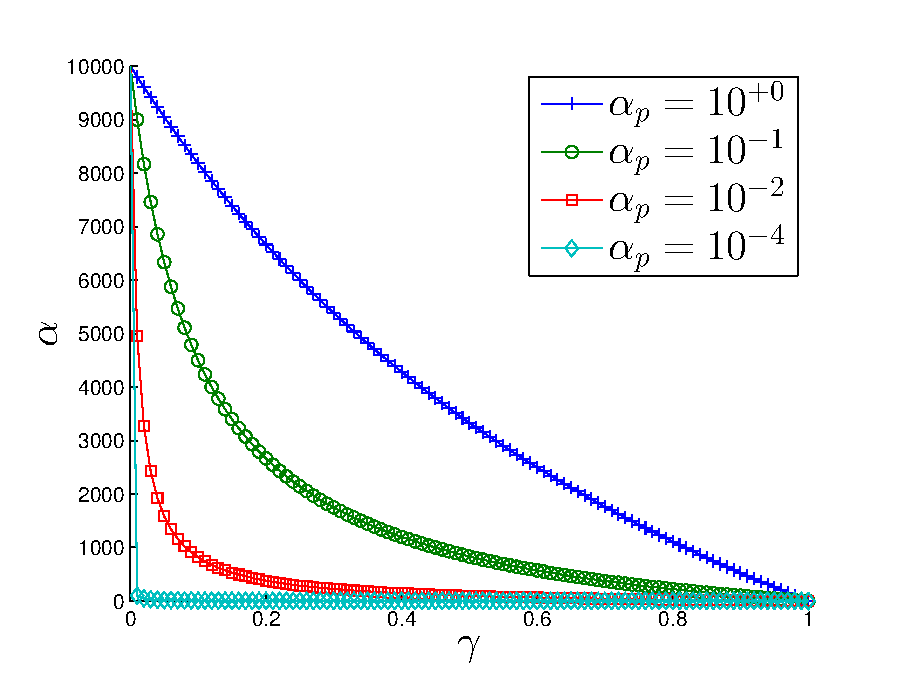
\includegraphics[scale=0.75]{alpha_convex.eps}
	\caption{Influence of the interpolation penalty $\alpha_{p}$.}
	\label{fig:alpha_convex}
\end{figure}
%
For more details on topology optimization of Stokes and Navier-Stokes flows, the reader is referred to \citep{Maute:14}.

% -----------------------------------------------------------------------------

\subsection{Discussion of the SIMP approach}
\label{sec:SIMP_discussion}

The concept of relating some artificial densities to the stiffness in structural problems can be expanded to other physics disciplines. The SIMP method can be used the describe material properties in thermal conductivity, magnetic permeability, porosity, etc.; and therefore, it found its way to a wide range of applications. The method requires a relatively small amount of iterations in order for the optimization problem to converge to an optimal design (at least for ``solid-void'' problems). SIMP has this capability because it operates on the entire design domain and not only on the boundaries; therefore, it does not suffer from localization effects. The approach is also suitable for a wide combination of design constraints, multiple load conditions, and extremely large (often 3D) systems. The educational article by \citet{Sigmund:01b} detailing a 99-line SIMP-code implemented in Matlab, as well as his web-based topology optimization program \citep{TS:01}\footnote{The software is now available on iOS phones and tablets.} played an important role in the acceptance of the SIMP method in both the academic and industry communities. Virtually all industrial optimization software uses the SIMP method as their optimization method of choice due to its ease of implementation.

% -----------------------------------------------------------------------------
% What are the disadvantages?

The SIMP method typically describes the interface between the different material domains either by using intermediate densities or by discrete material distributions, which may lead to jagged boundaries. In both cases, the representation of the interface is not precise, and therefore, the enforcement of boundary conditions at the interface is hindered. This may result in non-physical responses, such as premature yielding \citep{MSR:98} in structural mechanics, fluid flow penetrating solid material in low Reynolds number flow \citep{KPM:11}, and scalar fields diffusing through solid material at low P\'{e}clet number flow \citep{MPY+:12}. This issue can be mitigated by representing the material interface more accurately either by mesh refinement or adaptive re-meshing \citep{MR:95,MR:97}. However, for problems that require an accurate geometrical description of the interface, such as stresses in elasticity, boundary layer problems in fluids and skin-depth issues in electromagnetics, SIMP (and other material interpolation methods) will fail due to the jagged edges obscuring the physics \citep{ES:11,YNK+:11}.

Using material interpolation to address multi-material optimization problems is not a physics-based technique, and has been shown to violate the Hashin-Shtrikman bounds for low values of $\rho$ and large values of $p$ \citep{HS:62}. Furthermore, modeling multiple material phases can become complicated \citep{YA:01} and lead to slow convergence due to the larger number of iterations, as shown in \citep{VM:14}.

% -----------------------------------------------------------------------------
% Level set method

\section{Level set method}
\label{sec:intro_level_set_method}

The level set method applied to topology optimization arose as a technique capable of overcoming some of the shortcomings of the density approach. The main advantage of the method is that it allows for the description of complex geometries and the variation of the shape and topology of our design without introducing intermediate materials. A level set approach is a \textit{region-based} model with explicit boundaries, in contrast to the \textit{pixelated} model of the density method \citep{WW:04c}.

The level set method was first used to implicitly represent a structural boundary by \citep{OS:88}. Since then, it has been applied extensively in the field of imaging and computer visions \citep{OP:03}. The level set method eventually found its way to topology optimization, as the technique is well suited for the task: level set functions can form holes, split into multiple pieces, or merge with other level set functions \citep{WW:04c,AJT:02,OS:88}. 

The basic idea behind using the level set method to represent a shape boundary $\Gamma = \partial \Omega$ is to express a curve or surface as the zero level set of a higher dimensional implicit function $\phi$, as shown in Figures \ref{fig:level_set_circle_func_025}, \ref{fig:level_set_circle_func_050}, and \ref{fig:level_set_circle_func_075}, such that:
%
\begin{equation}
	\centering
	\label{eq:isolevel}
	\Gamma = \lbrace \mathbf{x} : \phi\left(\mathbf{x}\right) = 0 \rbrace
\end{equation}
%
Then we can divide the design domain into phase regions as:
%
\begin{equation}
	\centering
	\label{eq:level_set_regions}
	\begin{split}
		\phi\left(\mathbf{x}\right) > 0 & \quad \forall \mathbf{x} \in \Omega \backslash \partial \Omega \text{ (inside the region)} \\
		\phi\left(\mathbf{x}\right) = 0 & \quad \forall \mathbf{x} \in \partial \Omega \text{ (on the boundary)} \\
		\phi\left(\mathbf{x}\right) < 0 & \quad \forall \mathbf{x} \in D \backslash \Omega \text{ (outside the region)}
	\end{split}
\end{equation}
%
where $D$ represents the design domain, either bounded or unbounded, and contains all possible admissible shapes of $\Omega$, as shown in Figures \ref{fig:level_set_circle_domain_025}, \ref{fig:level_set_circle_domain_050}, and \ref{fig:level_set_circle_domain_075}. Each phase region may represent a different material \citep{AJT:02,WW:04c,OS:01,SW:00} or a different physics \citep{LCB:06,GW:08}. In the work of this thesis, the level set method is discretized with a finite element mesh.
%
\begin{figure}
	\centering
	\begin{tabularx}{\linewidth}{XX}
		\subfloat[]{
			\label{fig:level_set_circle_domain_025}
			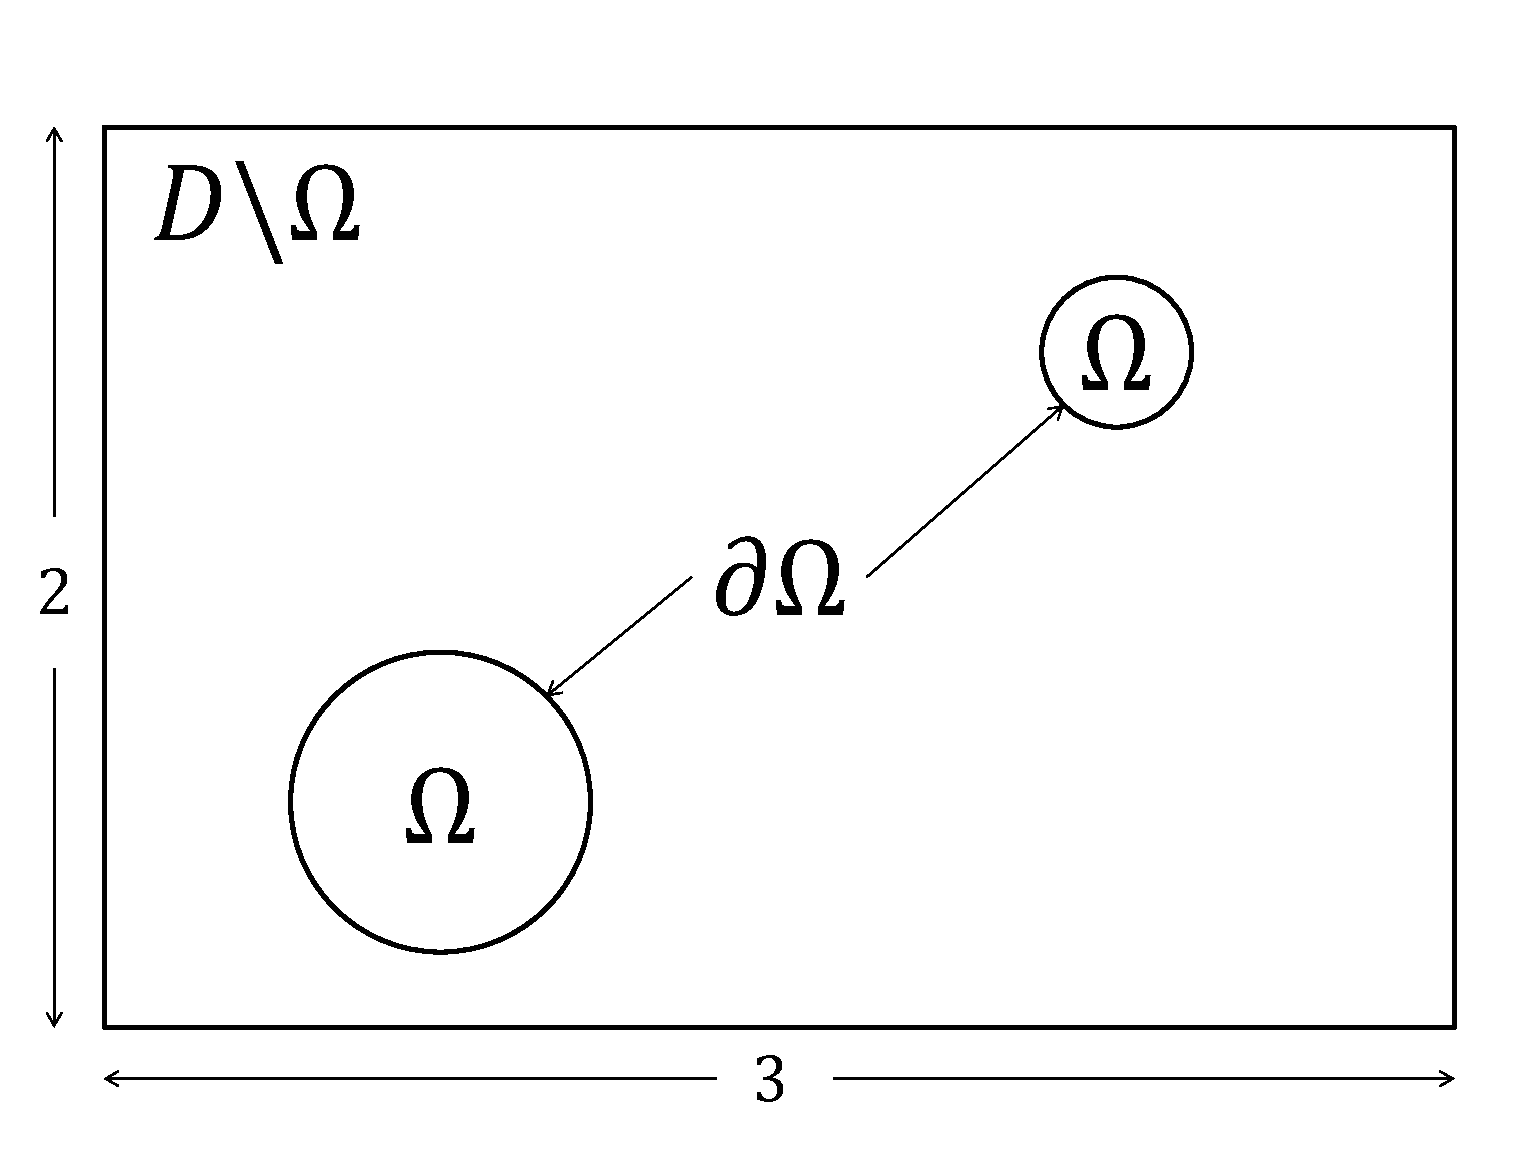
\includegraphics[width=\linewidth]{level_set_circles_1.eps}
		} &
		\subfloat[]{
			\label{fig:level_set_circle_func_025}
			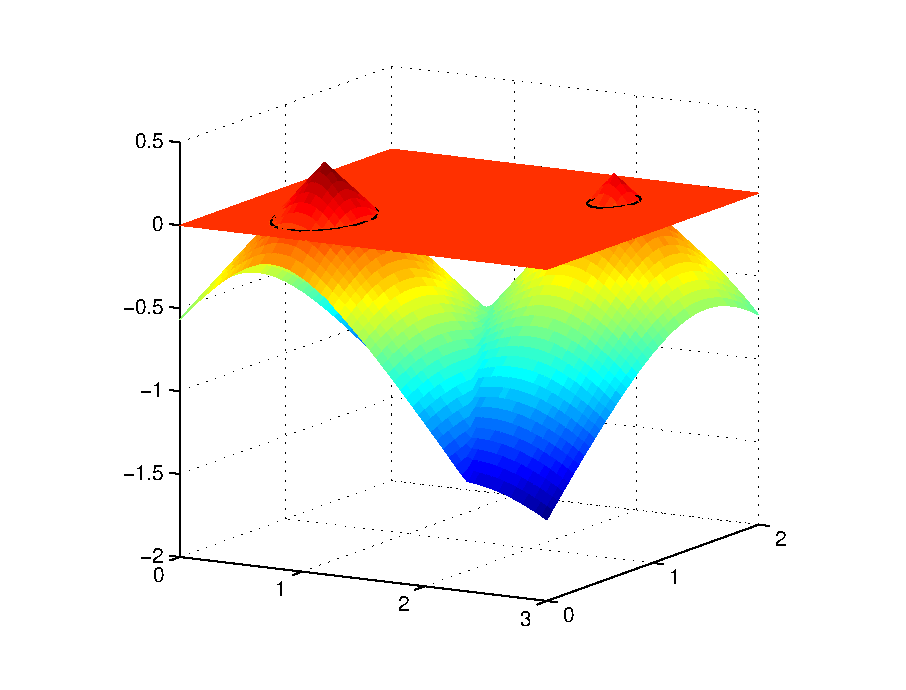
\includegraphics[width=\linewidth]{level_set_function_circles_1.eps}
		} \\
		\subfloat[]{
			\label{fig:level_set_circle_domain_050}
			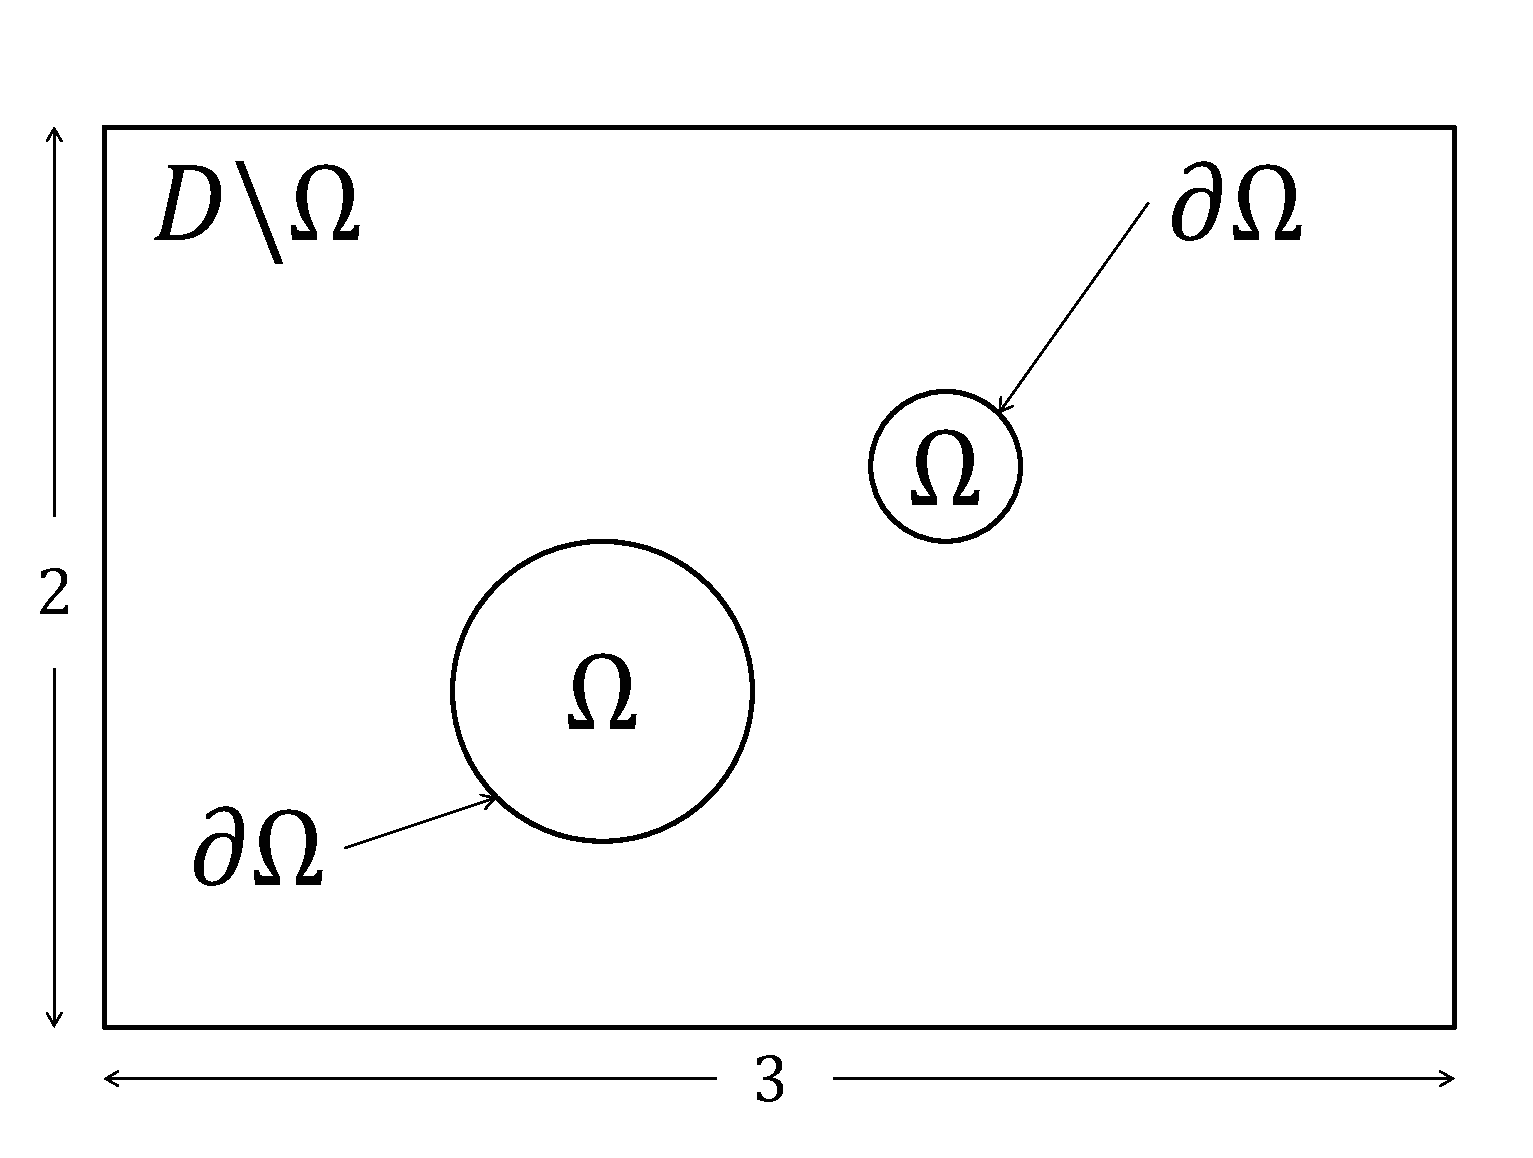
\includegraphics[width=\linewidth]{level_set_circles_2.eps}
		} &
		\subfloat[]{
			\label{fig:level_set_circle_func_050}
			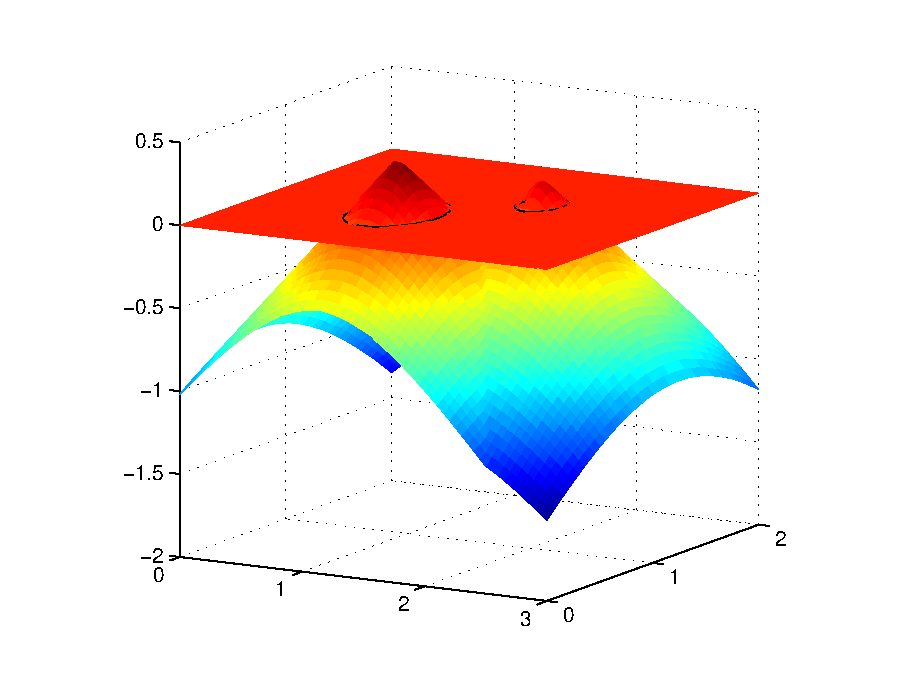
\includegraphics[width=\linewidth]{level_set_function_circles_2.eps}
		} \\
		\subfloat[]{
			\label{fig:level_set_circle_domain_075}
			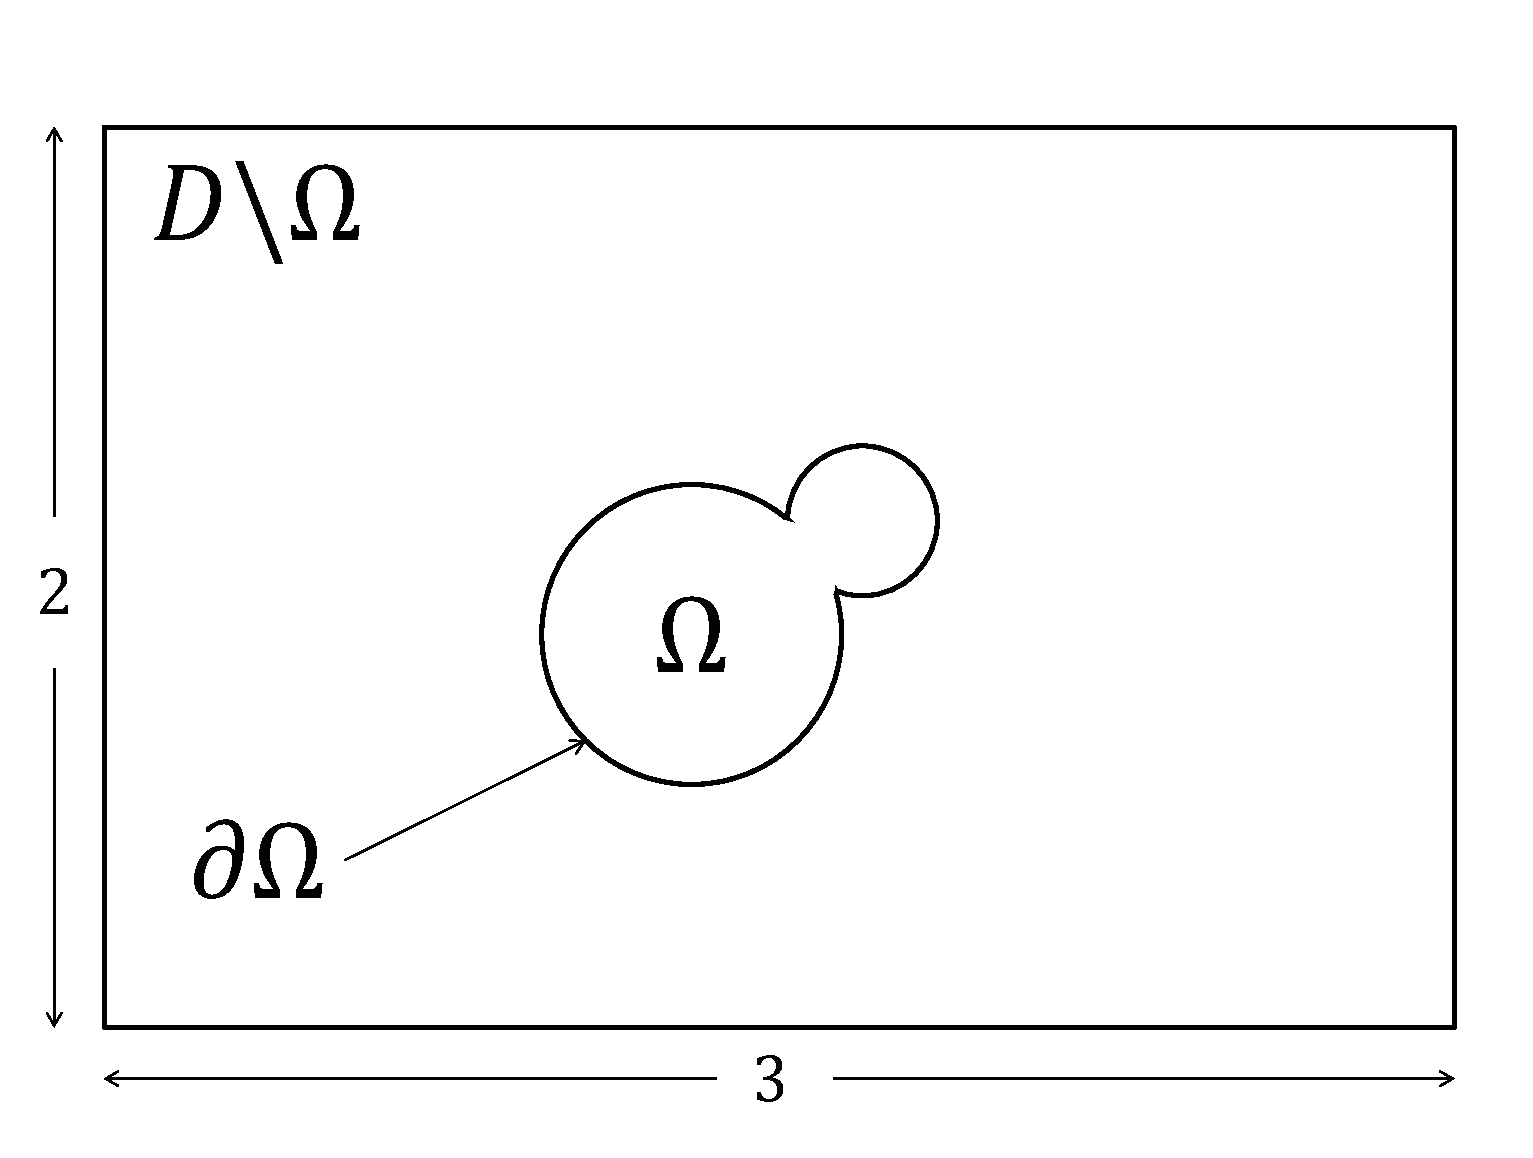
\includegraphics[width=\linewidth]{level_set_circles_3.eps}
		} &
		\subfloat[]{
			\label{fig:level_set_circle_func_075}
			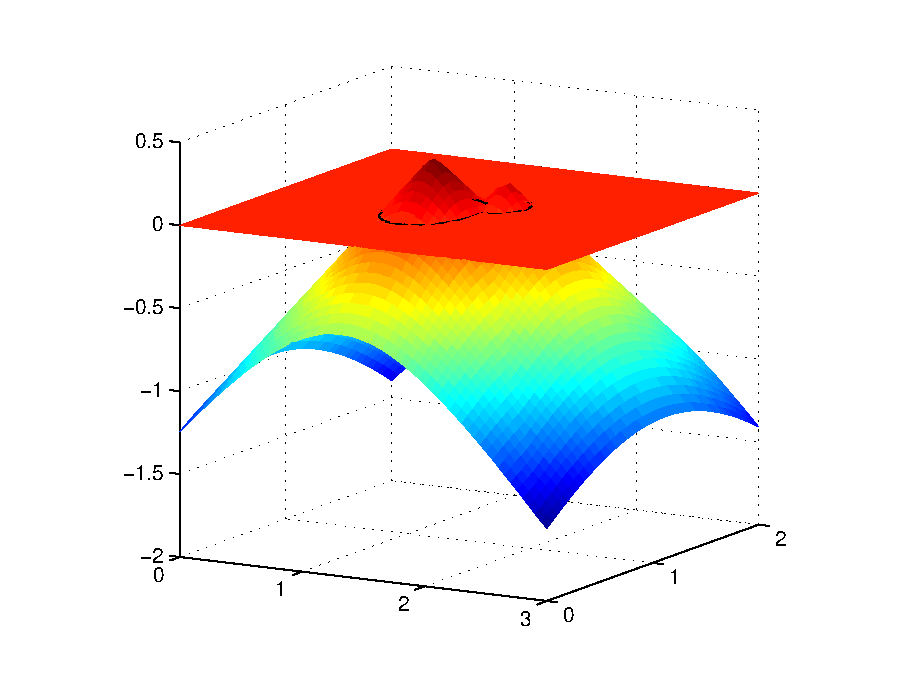
\includegraphics[width=\linewidth]{level_set_function_circles_3.eps}
		} \\
	\end{tabularx}
	\caption{Level set description of two circular inclusions with radii $0.667$ and $0.333$, respectively, moving towards each other. Level set functions can be used to describe complex topologies in a fixed mesh.}
	\label{fig:level_set_description}
\end{figure}

Multiple level set functions can be used to model more than two phase regions \ref{eq:level_set_regions}. As with the level set method itself, the use of multiple level set functions originated in image processing \citep{VC:02}. This so-called ``color'' level set method requires $m$ level set functions to model $n = 2^m$ different phase regions. For a reference on the method, the reader is referred to \citep{WW:04c,WW:05}.

The material distribution in the design domain can be determined from the phase region of the level set field. Several methods exists to describe this distribution. Density based level set methods describe the phase regions by either using element-wise constant material fractions or by mapping the level set field directly to a point \citep{YYK+:15}. These techniques are denoted as Ersatz material approaches (see Figure \ref{fig:ersatz_interpolation}) \citep{WWG:03,AJ+:05}, and while they ease the computational complexity, they lead to modeling errors. In this work, we will triangulate the element cut by the zero level set isolevel, and then perform our operations on the subdomains and on the interface (see Figure \ref{fig:XFEM_interpolation}) \citep{MM:13,VM:14}. This methodology will avoid the need to approximate material properties such as in density methods.

Regularization techniques are used in a level set optimization problem to control the geometry of the design. Among these techniques are perimeter or curvature minimization \citep{MKM+:11,YIN+:10,DLK:12}. The advantage of the level set method is that we possess a crisp definition of the phase interface, and therefore can integrate over the shape boundary $\Gamma_{\phi=0}$. These techniques will be studied in Section \ref{sec:topology_optimization_approaches_for_the_curvature_minimization_of_level_set_isocontours}.

% -----------------------------------------------------------------------------
% Topology optimization with the level set method

\subsection{Topology optimization with the level set method}

The topology of the level set field is modified by update schemes that use the sensitivities of the design variables. Several approaches exist, such as the Hamilton-Jacobi equation \citep{YNY+:10}. This work will focus on a mathematical programming approach, where the nodal values of the discrete level set field are defined as functions of the optimization design variables. Like in the filtering method of density approaches, we will define a linear filter
%
\begin{equation}
	\label{eq:smoothing_filter_XFEM}
	\phi\left(\mathbf{s}\right)=\frac{\sum_{i=1}^{N}w_{i}s_{i}}{\sum_{i=1}^{N}w_{i}}
\end{equation}

with

\begin{equation}
	\label{eq:weight_XFEM}
	w_{i}=\max \left( 0, r_{\phi} - \Vert \mathbf{x}_i - \mathbf{x} \Vert \right)
\end{equation}
%
where $\phi\left(\mathbf{s}\right)$ is the level set function at a point $\mathbf{x}$, $\mathbf{x}_{i}$ is the location of the node at which the design variable $i$ is defined, $w_{i}$ is the factor of point $\mathbf{x}$ with respect to the design variable $i$, $r_{\phi}$ is the filter radius, and $N$ is the number of nodes in the design domain. However, unlike the filter in the density approaches, this filter cannot control the minimum feature size, as discussed in Section \ref{sec:feature-size-control}.

The reader is referred to \citep{DML+:13,GP:13} for a more detailed overview of the level set method and topology optimization approaches.

% -----------------------------------------------------------------------------
% Extended finite element method

\section{Extended finite element method}
\label{sec:intro_xfem}

The extended finite element method (XFEM) is an immersed boundary technique that works on fixed meshes. The XFEM was built upon the concept of partition of unity developed by \citep{NME:NME86}, and it was originally used to model crack propagation \citep{BB:99}. Due to its ability to approximate discontinuous solutions, the method has been applied in a variety of discontinuous partial differential equations, such as multimaterial structural mechanics \citep{WW:04c,VM:14}, fluid-structure interaction \citep{GW:08}, and multi-phase flows \citep{CB:03}. The method has also been applied to shape optimization by \citep{DMJ+:06,MMF+:05,MD:07}, and to topology optimization by \citep{HMM:13,LWW:12,WWX:10,MKM+:11,MM:14,VM:14}.

The XFEM decomposes the cut elements into subdomains and interfaces that it uses to integrate the weak form of the governing equations. Figure \ref{fig:triangulation_2D} illustrates this by showing the possible decompositions of a two dimensional finite element based on its nodal level set values.
%
\begin{figure}
	\centering
	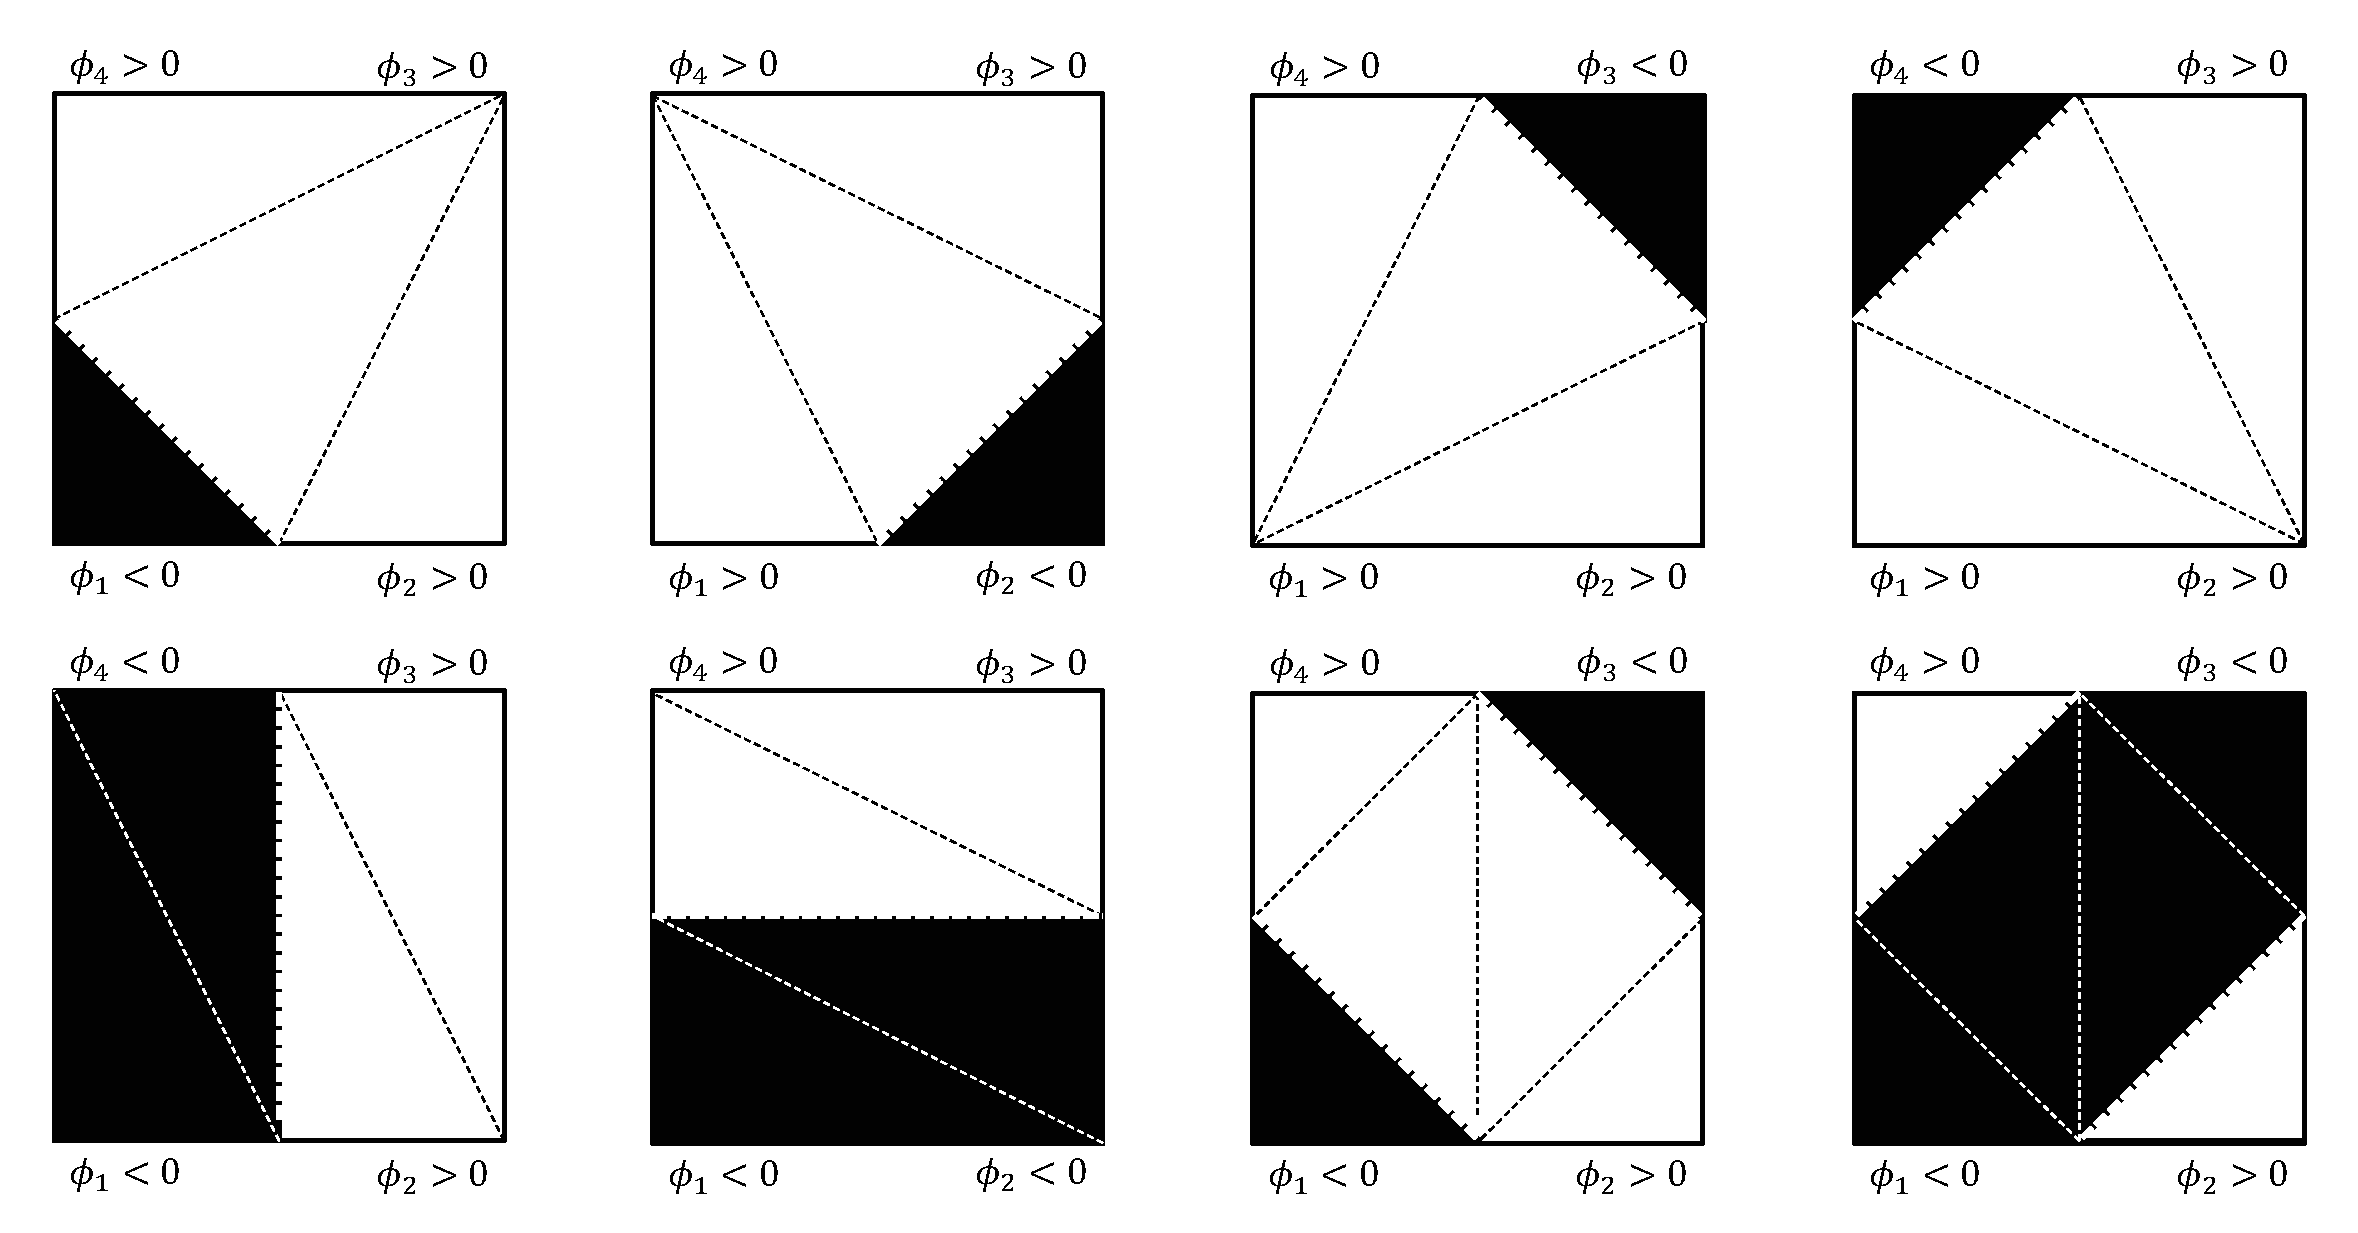
\includegraphics[width=\linewidth]{intersections_2D.eps}
	\caption{A two dimensional finite element has eight possible decompositions based on the nodal level set values.}
	\label{fig:triangulation_2D}
\end{figure}

The XFEM can model discontinuities in the solution field by augmenting the standard finite element function space with additional degrees-of-freedom, denoted ``enriched degrees-of-freedom''. To illustrate this with a quick example, consider an XFEM model that consists of a two dimensional mesh with four linear elements. The level-set distribution in Figure \ref{fig:intro_structural_model} leads to the intersection pattern shown in Figure \ref{fig:intro_physical_model}. The nodes on the left are clamped, and the right edge is subject to a constant pressure load. The node at the center of the mesh in Figure \ref{fig:intro_physical_model} will use different degrees-of-freedom to interpolate the different subdomains, and avoid artificially coupling the disconnected phase regions.
%
\begin{figure}
	\centering
	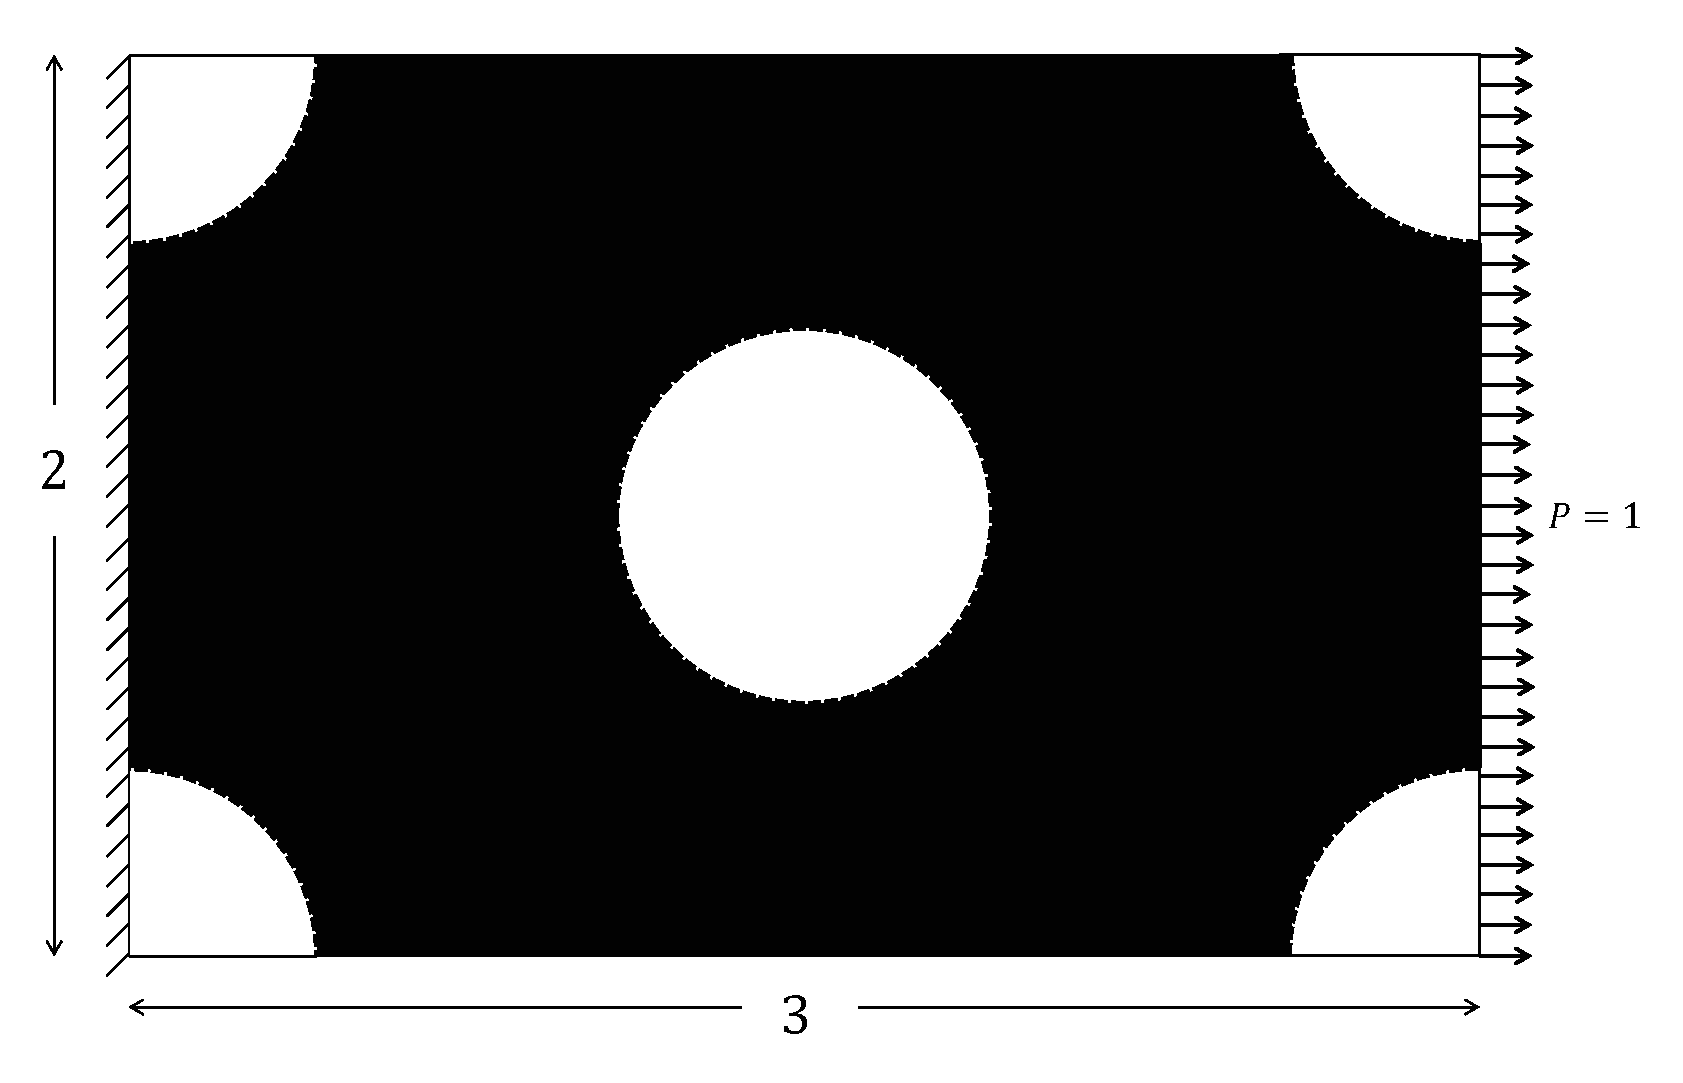
\includegraphics[width=0.75\linewidth]{structural_model.eps}
	\caption[Structural problem setup.]{Structural problem setup. The domain contains multiple level set inclusions.}
	\label{fig:intro_structural_model}
\end{figure}
%
\begin{figure}
	\centering
	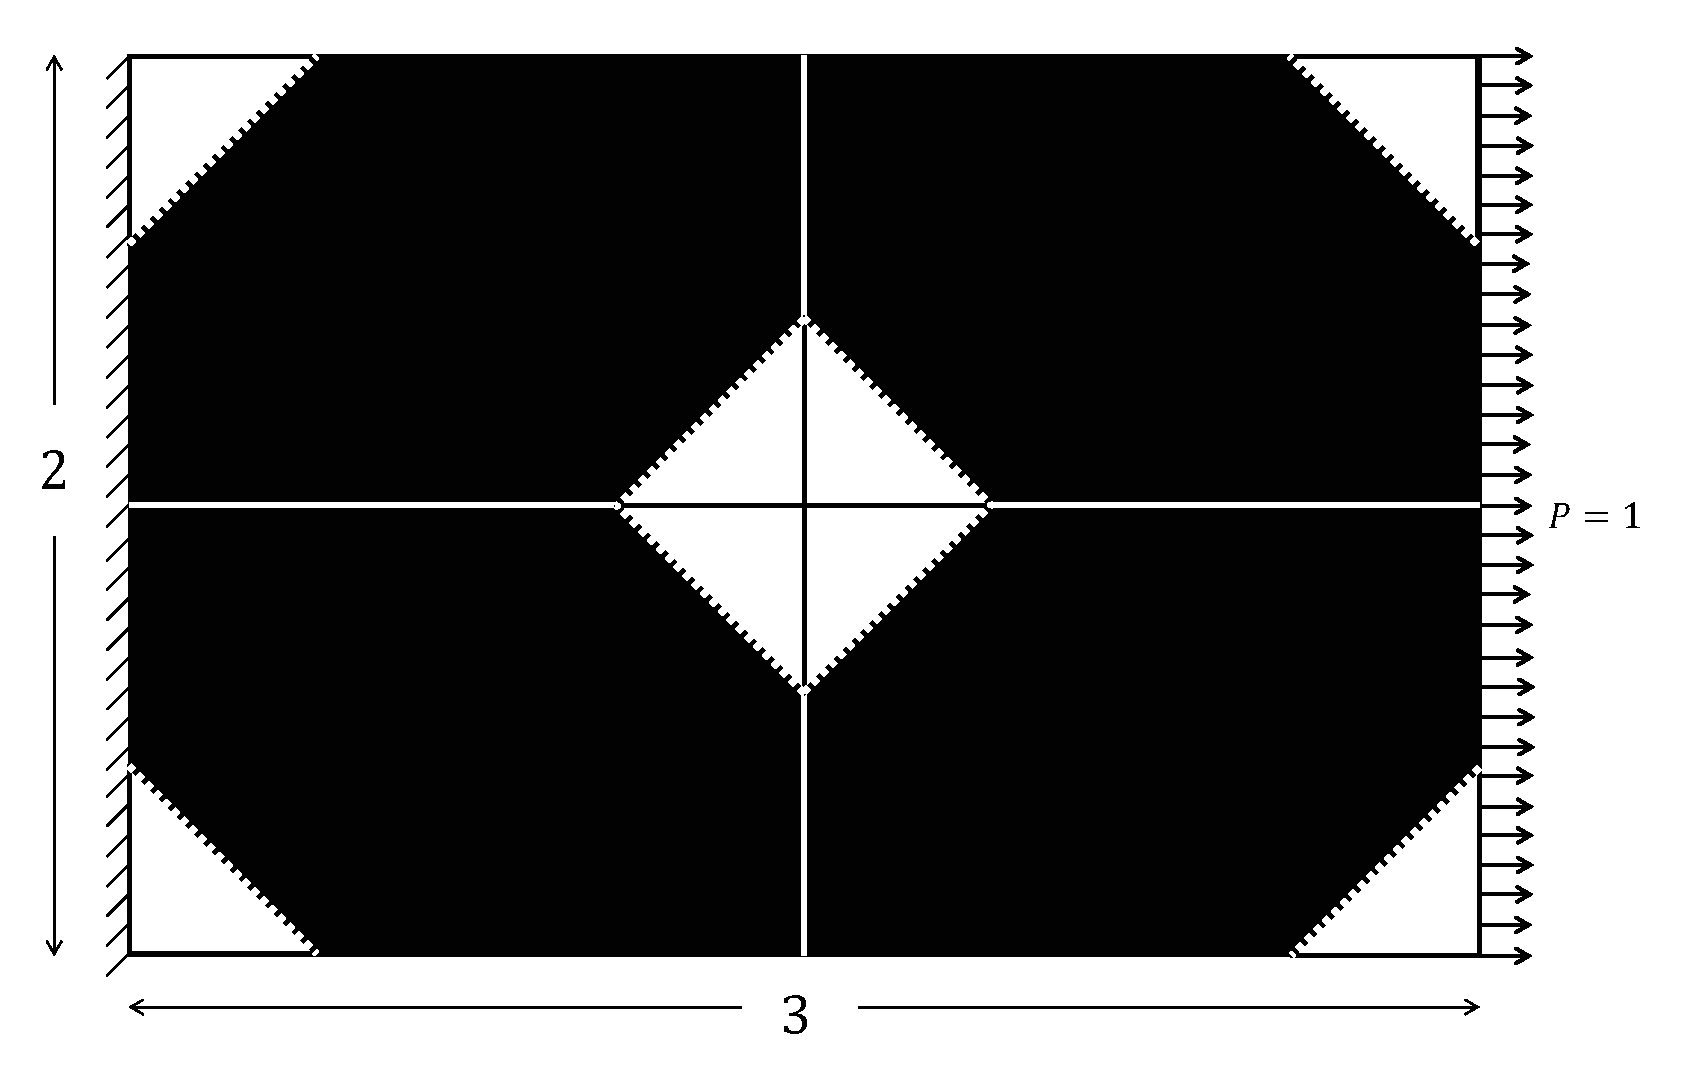
\includegraphics[width=0.75\linewidth]{physical_model.eps}
	\caption[XFEM implementation example physical model]{4-element 2D mesh. Black areas: material phase 1, negative level-set value at the nodes; white areas: material phase 2, positive level-set value.}
	\label{fig:intro_physical_model}
\end{figure}

The solution space is then interpolated using the generalized enrichment formulation of \citep{HH:04}:
%
\begin{equation}
	\mathbf{u}(\mathbf{x}) = \sum \limits^{M}_{m=1} \left( H(-\phi) \sum\limits^{n}_{i=1} \mathbf{N}_i \ \mathbf{u}_{i,m}^A
														 + H( \phi) \sum\limits^{n}_{i=1} \mathbf{N}_i \ \mathbf{u}_{i,m}^B \right)
\end{equation}

where $m$ is the enrichment level, $M$ is the maximum number of enrichment levels used for each phase, $\mathbf{N}$ are the shape functions, $\mathbf{u}^l_{i,m}$ is the vector of degrees-of-freedom values at node $i$ for phase $l=[A,B]$, $\phi$ is the level set value evaluated at $\mathbf{x}$, and $H$ denotes the Heaviside function. This is illustrated in Figure \ref{fig:intro_enrichment_model} for the structural problem of Figure \ref{fig:intro_structural_model}.
%
\begin{figure}[htbp]
	\centering
	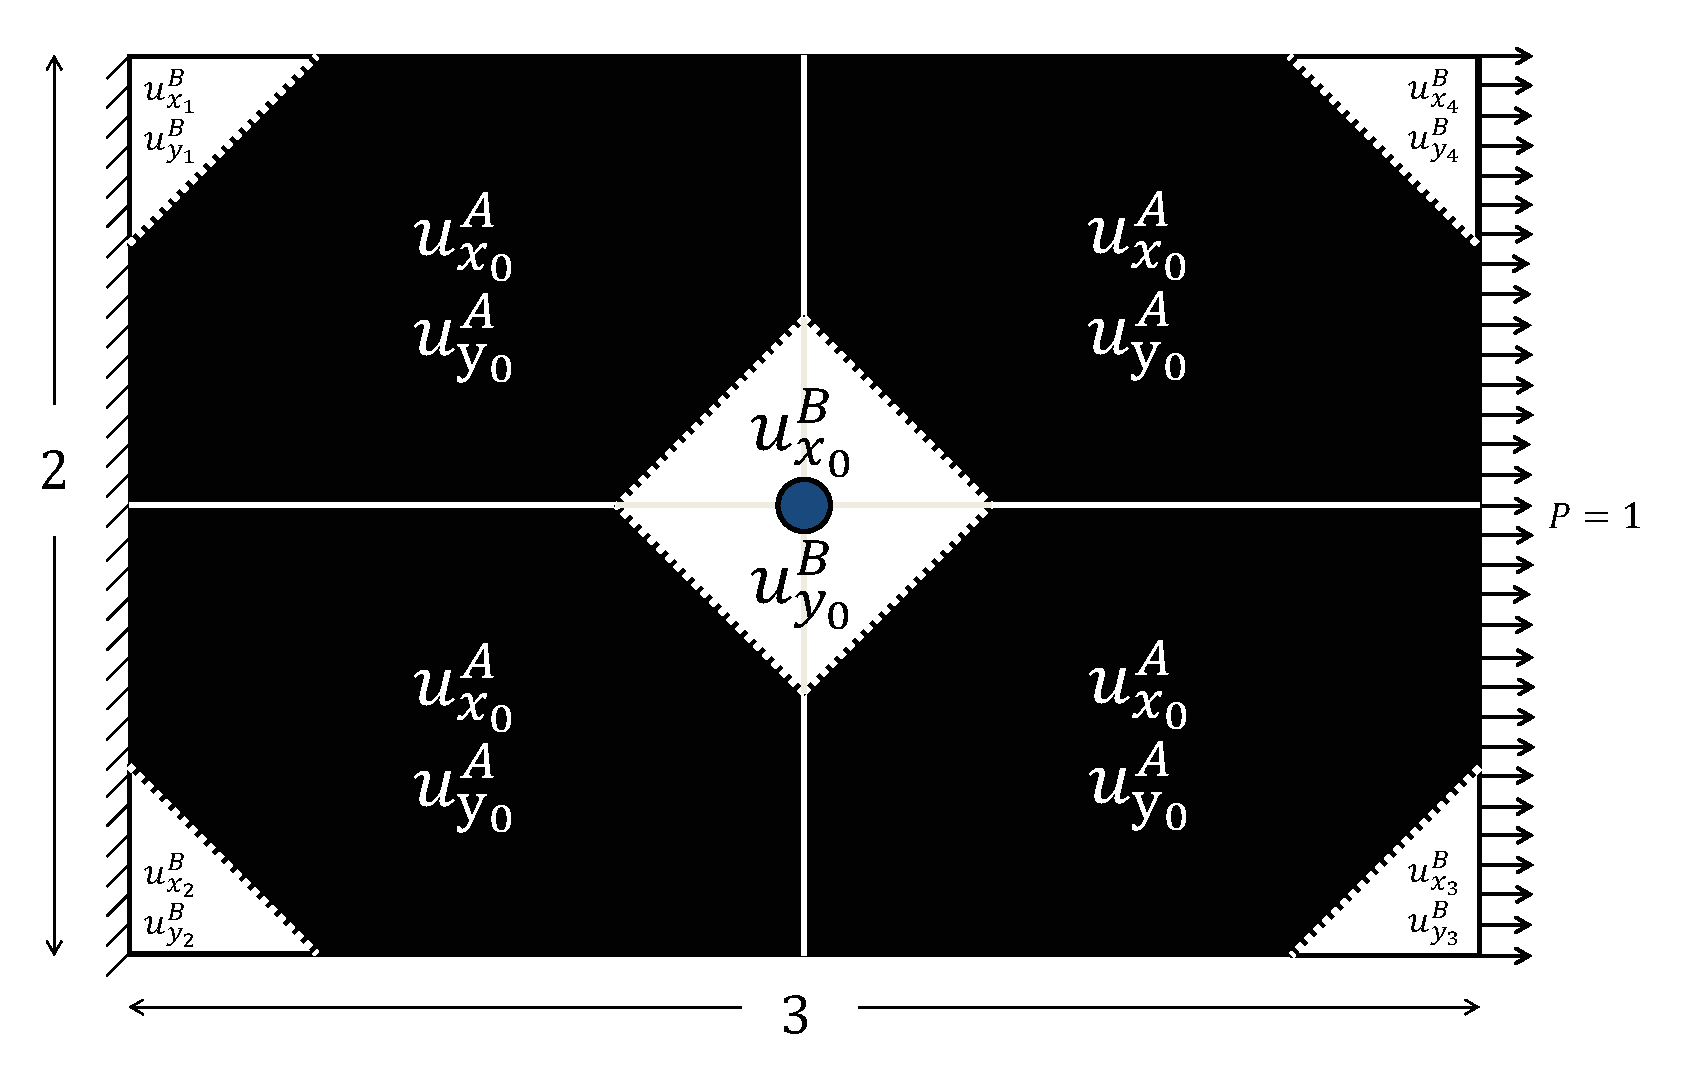
\includegraphics[width=0.9\linewidth]{enrichment_model.eps}
	\caption{The center node, denoted by the color blue, uses different degrees-of-freedom to describe the disconnected phase regions. The subscripts denote the $m$ enrichment level. The maximum number of enrichment levels used for each phase is $M=5$. A value of 0 denotes the original finite element degrees-of-freedom, while other numbers indicate additional ``enriched degrees-of-freedom''. }
	\label{fig:intro_enrichment_model}
\end{figure}

The Heaviside function $H$ depends on the level set function and is defined as follows:
%
\begin{equation}
	H(z) =
		\begin{cases}
			1 & z > 0 \\
			0 & z \le 0
		\end{cases}
\end{equation}

The Heaviside functions ``turns on/off'' the standard finite element interpolations in the particular phases. The approximation allows for discontinuities of the states $\mathbf{u}$ along the phase boundaries. Therefore, the continuity of the solution at the interface between different phase regions must be enforced. Several techniques are available in the literature, such as stabilized Lagrange multipliers (Section \ref{sec:density_and_level_set_XFEM_schemes_for_topology_optimization_of_3D_structures}) \citep{BH:10}, and the Nitsche method (Section \ref{sec:level_set_XFEM_topology_optimization_of_3D_navier_stokes_and_scalar_transport_problems}) \citep{BH:12}. More recent development include the face-oriented ghost penalty (Section \ref{sec:level_set_XFEM_topology_optimization_of_3D_navier_stokes_and_scalar_transport_problems}) by \citep{SW:14,SRG+:14,BH:12}, which aims at smoothing the gradients of the solution between cut elements. All three formulations will be studied and applied to topology optimization in this work.

For more details, refer to Sections \ref{sec:a_complete_methodology_for_the_implementation_of_XFEM_inclusive_models}, \ref{sec:discretization}, and \ref{sec:computational-considerations}. For a review of the XFEM, the user is referred to \citep{FB:10}.

% -----------------------------------------------------------------------------
% Available software

% \section{Available software}

% For the numerical modeling and simulation, we will use our in-house code, the Finite Element Multidisciplinary Optimization Code (FEMDOC). The linear algebra package is provided by Trilinos \citep{Trilinos:03}.

% -----------------------------------------------------------------------------
%
%* What is your work about?
%
%- Topology optimization approach.
%- Using the Level Set Method.
%- eXtended Finite Element Method.
%- LSM describes the geometry of the design.
%- XFEM is used to solve the PDE and measure the performance.
%- Apply methodology for complex work.
%
%* Who should care about your work?
%
%- Topology optimization community. 
%- Alternate method to homogenization methods.
%- Design engineers.
%- Surface mesh ready for three dimensional printing.
%
%* What are the goals of your thesis?
%
%- Develop robust topology optimization approach using the LSM and the XFEM methods.
%- Compare pros and cons against homogenization methods.
%- Apply methodology to real-world problem, such as ALD.
%
%* What is your overarching approach? How will you know you have accomplished your goals?
%
%- Develop methodology for triangulation, enrichment of 3D geometries (methodology section).
%- Test framework with structural problems in three dimensions (structural section).
%- Compare results with SIMP (structural section).
%- Expand to incompressible Navier-Stokes and Stokes flows, and scalar transport (fluids section).
%- Study convergence with respect to the enforcement of boundary conditions to ensure stability and coercivity.
%- Study convergence with respect to intersection configuration.
%- Study shape control and regularization techniques (curvature section).
%- Three dimensional printing (structural, fluids, curvature sections).
%- Apply methodology to ALD problem (ALD section).
%
%* Why should they care about your work?
%
%- Methodology accommodates different physics.
%- Accommodate structural, Navier-Stokes, scalar transport physics.
%- Three dimensional problems.
%- For topology optimization, it is relevant because it provides an alternate method besides homogenization methods.
%- Advantages over SIMP.
%- Explicit description of boundary for correct application of boundary conditions.
%- Regularization techniques allow shape control of the interface.
%- Prevents spurious diffusion, etc.
%- Coarser mesh leads to faster computations.
%
%* Does it enable us to solve new optimization problems or just live with coarser mesh?
%
%- Solve topology optimization problems where physics at interface is crucial.
%- ALD requires measuring temperature distribution correctly. Spurious diffusion does not help the problem.
%- Coarse mesh is good enough to describe physics at the interface.
%- In 3D, efficiency is crucial.
%
%* How is thesis proposal structured?
%
%- What sections present?
%- Mention sections are drafts of papers.

% -----------------------------------------------------------------------------
% A complete methodology for the implementation of XFEM inclusive models.

\chapter{A complete methodology for the implementation of XFEM inclusive models}
\label{sec:a_complete_methodology_for_the_implementation_of_XFEM_inclusive_models}

% -----------------------------------------------------------------------------
% Abstract.

This document was written in 2012 as an internal implementation manual for future developers of our code, the Finite Element Multi-Disciplinary Optimization Code (femdoc).

This report offers a background into the eXtended Finite Element Method as a tool to solve the shortcomings of the classical Finite Element Method. An example of such is the numerical solution to problems with different material topologies (i.e. discontinuities). The XFEM uses level set functions to track the location of these discontinuities. The report also provides algorithms for locating these discontinuities and subsequently dividing the domain into sub-domains capable of integration. This report ultimately expounds upon how to effectively apply the local enrichment functions that the XFEM standard approximation requires at the nodes where the discontinuities occur.

The reader may skip this section, as it focuses on the algorithmic implementation of the framework and most of its content is intended for software developers.

% -----------------------------------------------------------------------------
% Chapters.

% XFEM: Background.
\chapter{Introduction}
\label{sec:introduction}

The goal of this thesis proposal is to introduce a unified topology optimization framework that uses the \textbf{L}evel \textbf{S}et \textbf{M}ethod (LSM) to describe the design geometry and the e\textbf{X}tended \textbf{F}inite \textbf{E}lement \textbf{M}ethod (XFEM) to solve the governing equations and measure the performance of the design. The framework will be referred to as the LSM-XFEM optimization method.

Topology optimization approaches (see Sections \ref{sec:optimization} and \ref{sec:intro_topology_optimization}) seek the optimal geometry and/or material layout of a body within a given design domain. Popular schemes, such as density methods (Section \ref{sec:density_topology_approaches}), have been widely applied to topology optimization of different physics, such as structures, fluid dynamics, etc. In structural topology optimization, the density method works by transforming the structural optimization problem into a standard nonlinear program where the design variables are coefficients of the governing equation. These design variables are introduced as the material density of the finite elements. Density approaches cannot describe the physics at the phase interface accurately without extensive mesh refinement. This may lead to unphysical responses (Section \ref{sec:SIMP_discussion}). Therefore, problems that require an accurate description of the boundary conditions at the interface may not be suited for density approaches.  The use of level set methods in topology optimization emerged as an alternative to the density approach. Level set methods (Section \ref{sec:intro_level_set_method}) are able to provide an accurate representation of the layout by dividing the design domain into phase regions, where each region may represent a different physics or a different material, as shown in Figure \ref{fig:level_set_circle_description}.
%
\begin{figure}
	\centering
	\begin{tabularx}{\linewidth}{XX}
		\subfloat[]{
			\label{fig:level_set_circle_func_1}
			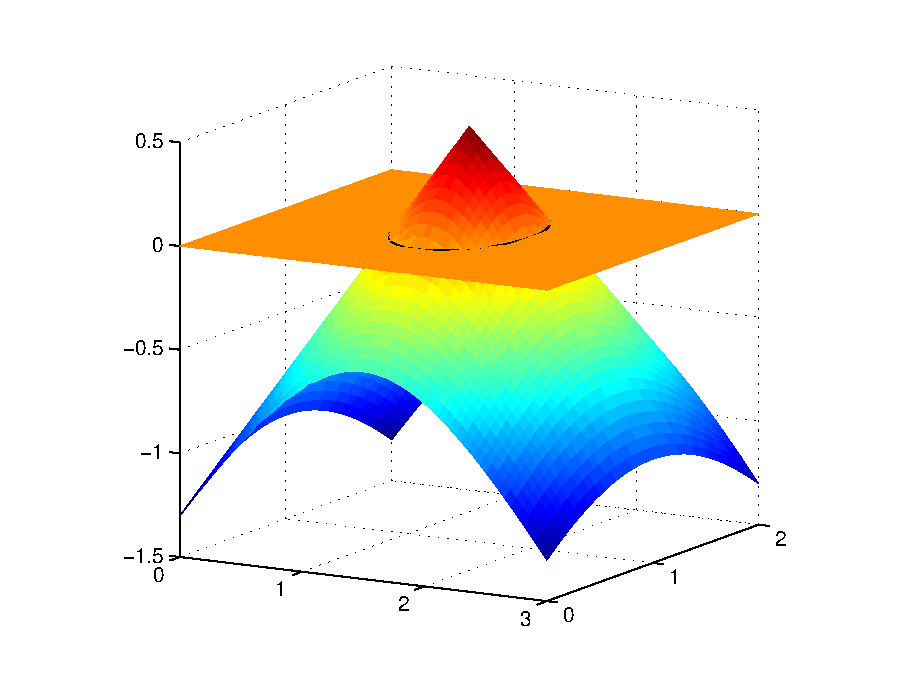
\includegraphics[width=\linewidth]{level_set_circle_func_050.eps}
		} &
		\subfloat[]{
			\label{fig:level_set_circle_domain_1}
			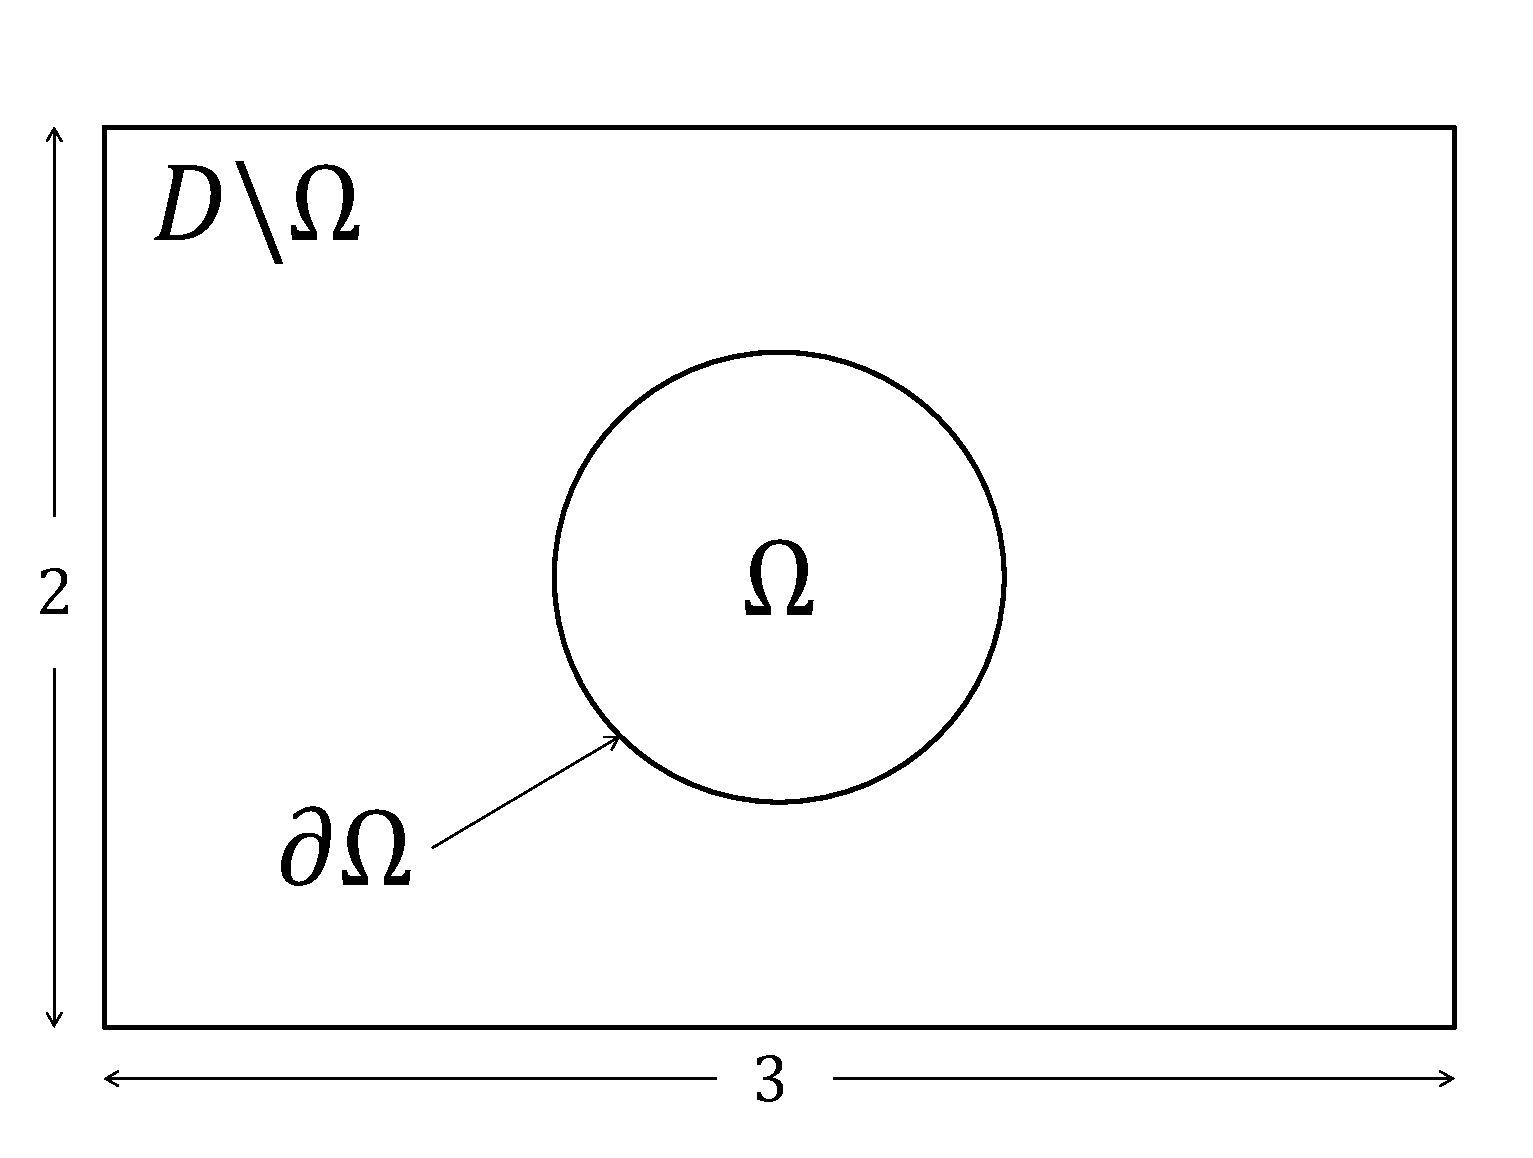
\includegraphics[width=\linewidth]{level_set_circle_domain_050.eps}
		}
	\end{tabularx}
	\caption{The zero level set isolevel of the level set function, $\partial \Omega = \Gamma_{\phi=0}$, in \ref{fig:level_set_circle_func_1} divides the fixed mesh grid into different phase regions in \ref{fig:level_set_circle_domain_1}, where each phase may represent a different material or a different physics.}
	\label{fig:level_set_circle_description}
\end{figure}

To illustrate the differences in the geometry representation between the density and level set methods, consider the ``solid-void'' structural optimization problem presented in Figure \ref{fig:structural_compliance_setup}, where the objective is to minimize the structural compliance by changing the material layout, subject to a maximum volume fraction of 0.5 for the solid phase. The results for both the density and level set approaches are shown in Figure \ref{fig:structural_compliance_comparison}. Notice both designs generate similar truss-like geometries. Figure \ref{fig:structural_compliance_comparison_SIMP} shows how the density method represents the interface between the solid and void materials as intermediate ``grey'' densities, while the level set method in Figure \ref{fig:structural_compliance_comparison_XFEM} describes the geometry by cutting the elements.
%
\begin{figure}[H]
	\centering
	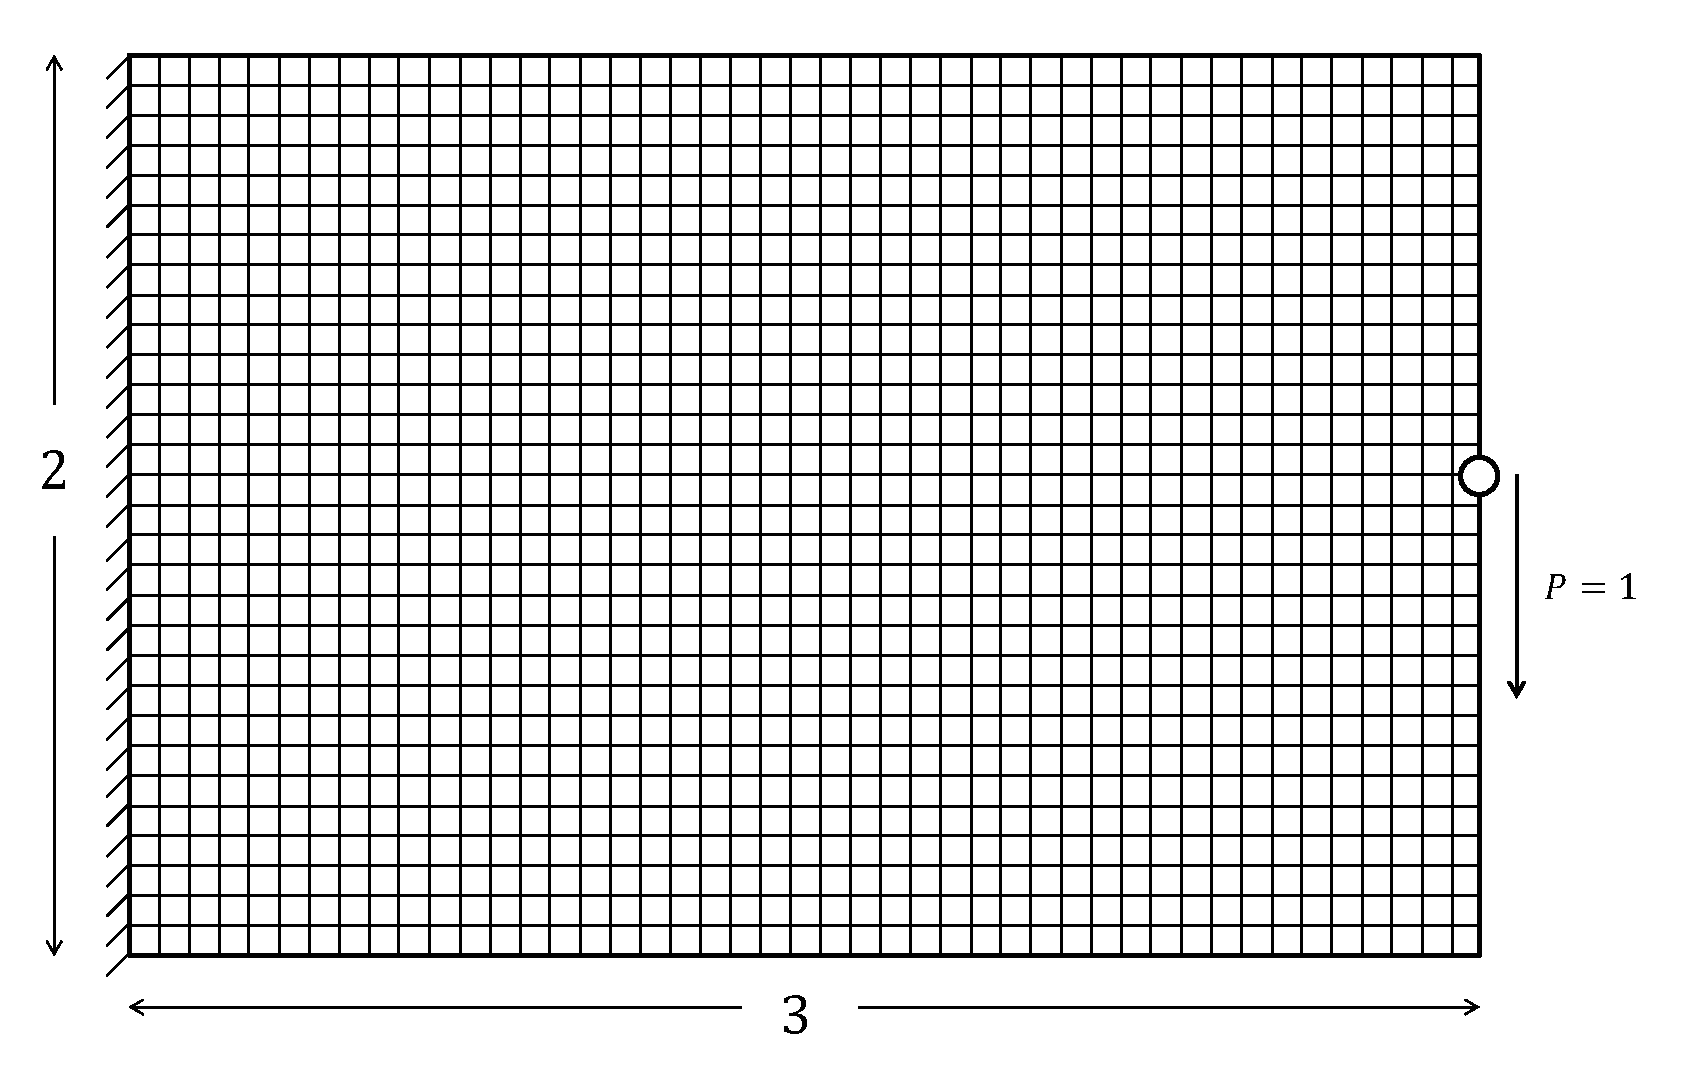
\includegraphics[scale=0.4]{structural_compliance_setup.eps}
	\caption{Setup of a structural topology optimization problem. A mesh of size $3L \times 2L$, with $45 \times 30$ quadrilateral linear elements is anchored to the wall on its left side, and subject to a point load on its right side.}
	\label{fig:structural_compliance_setup}
\end{figure}
%
\begin{figure}[H]
	\centering
	\begin{tabularx}{0.75\linewidth}{X}
		\subfloat[Density method.]{
			\label{fig:structural_compliance_comparison_SIMP}
			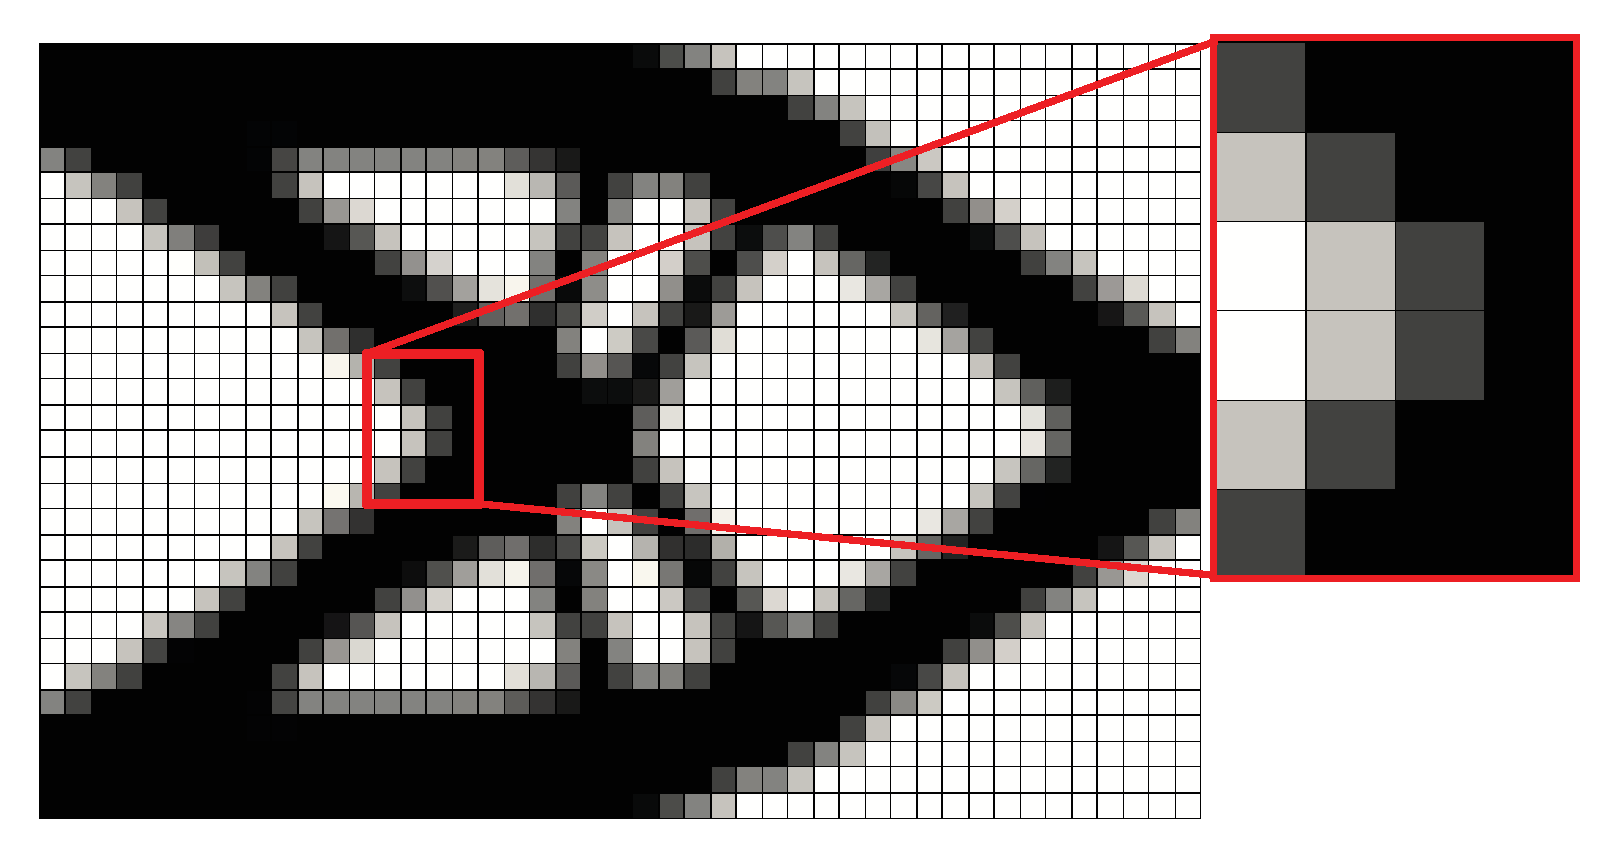
\includegraphics[width=\linewidth]{structural_compliance_comparison_SIMP.eps}
		} \\
		\subfloat[Level set method.]{
			\label{fig:structural_compliance_comparison_XFEM}
			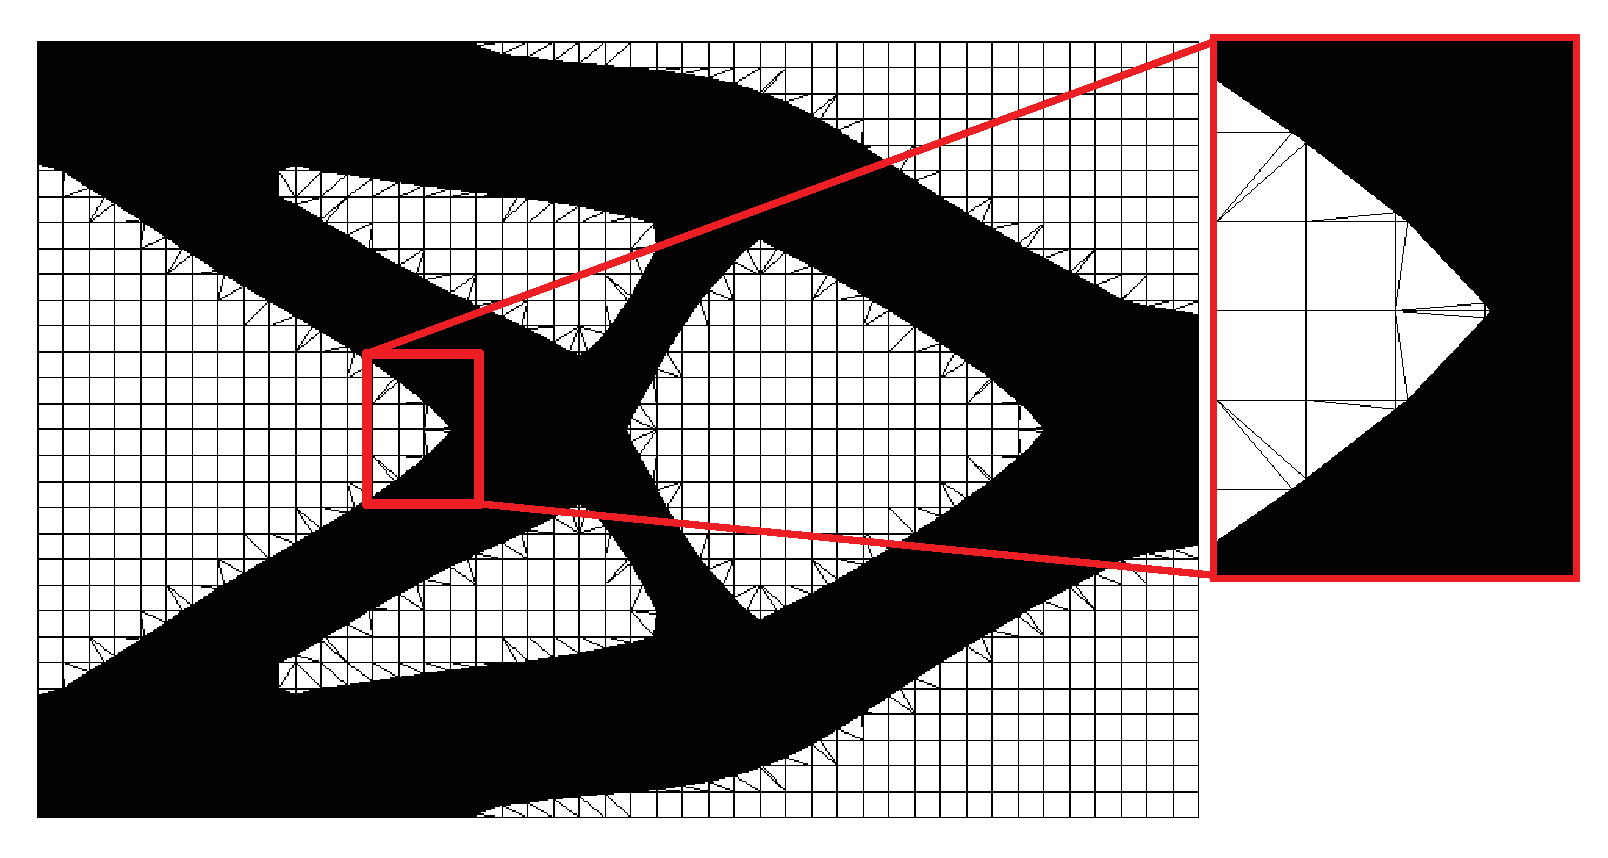
\includegraphics[width=\linewidth]{structural_compliance_comparison_XFEM.eps}
		}
	\end{tabularx}
	\caption{Comparison of the geometry representation of the density and level set methods for a ``solid-void'' structural topology optimization problem.}
	\label{fig:structural_compliance_comparison}
\end{figure}

In the level set method, the material properties of the structural finite elements are interpolated between the void and solid phases, proportional to the volumes of the individual phases. This approach is called Ersatz material interpolation and it is very similar to the interpolation used in density methods. Therefore, it leads to similar issues with regard to enforcing boundary conditions and predicting the physical response along the boundary. The process is illustrated in Figure \ref{fig:ersatz_interpolation}.
%
\begin{figure}[H]
	\centering
	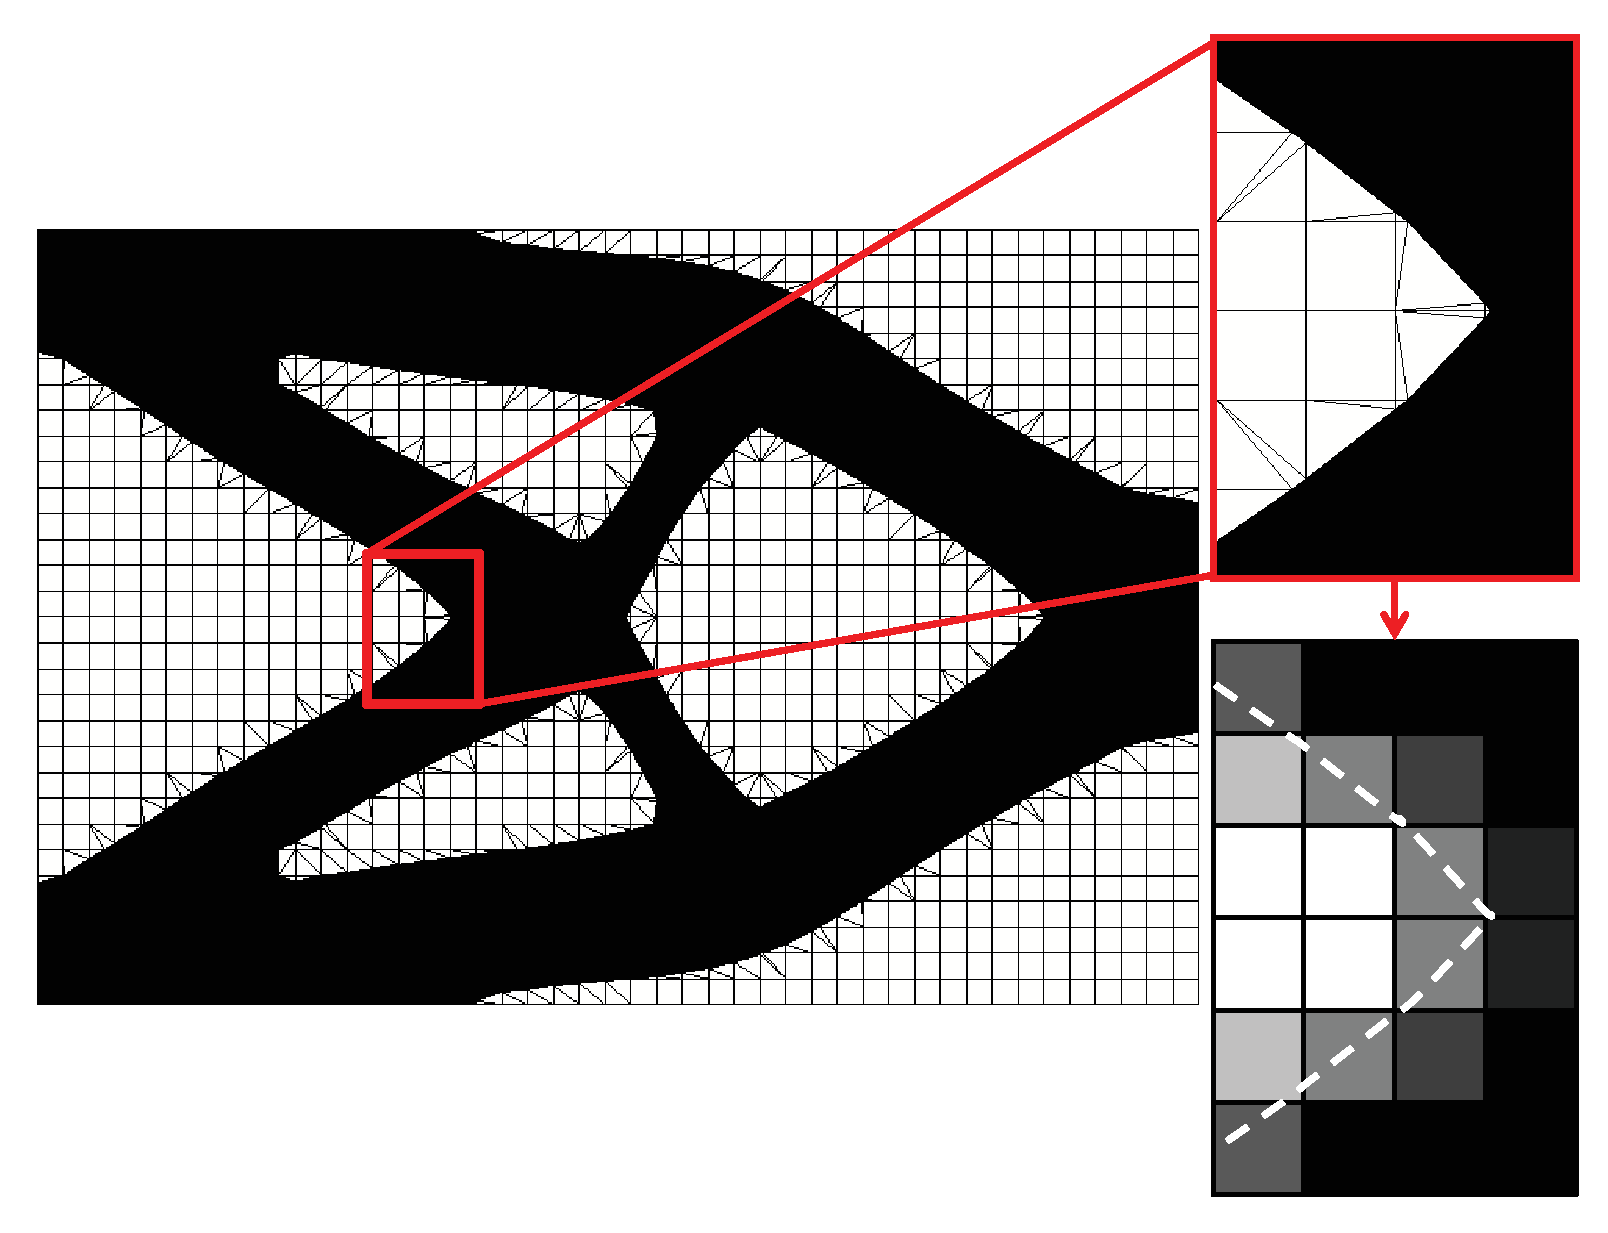
\includegraphics[scale=0.4]{ersatz_interpolation.eps}
	\caption{In an Ersatz material interpolation approach, the material properties of each finite element are interpolated proportional to the volumes of the solid and void phases.}
	\label{fig:ersatz_interpolation}
\end{figure}

An alternative to the Ersatz interpolation is to repeatedly generate new meshes that align with the geometry of the zero level set isolevel, as shown in Figure \ref{fig:remeshing_interpolation}. However, generating an entirely new body fitted
mesh typically suffers from robustness and efficiency, particularly for three dimensional problems. It was also shown by \citep{SMR:00} and \citep{WKG:06} that this method affects the convergence of the optimization process.
%
\begin{figure}[H]
	\centering
	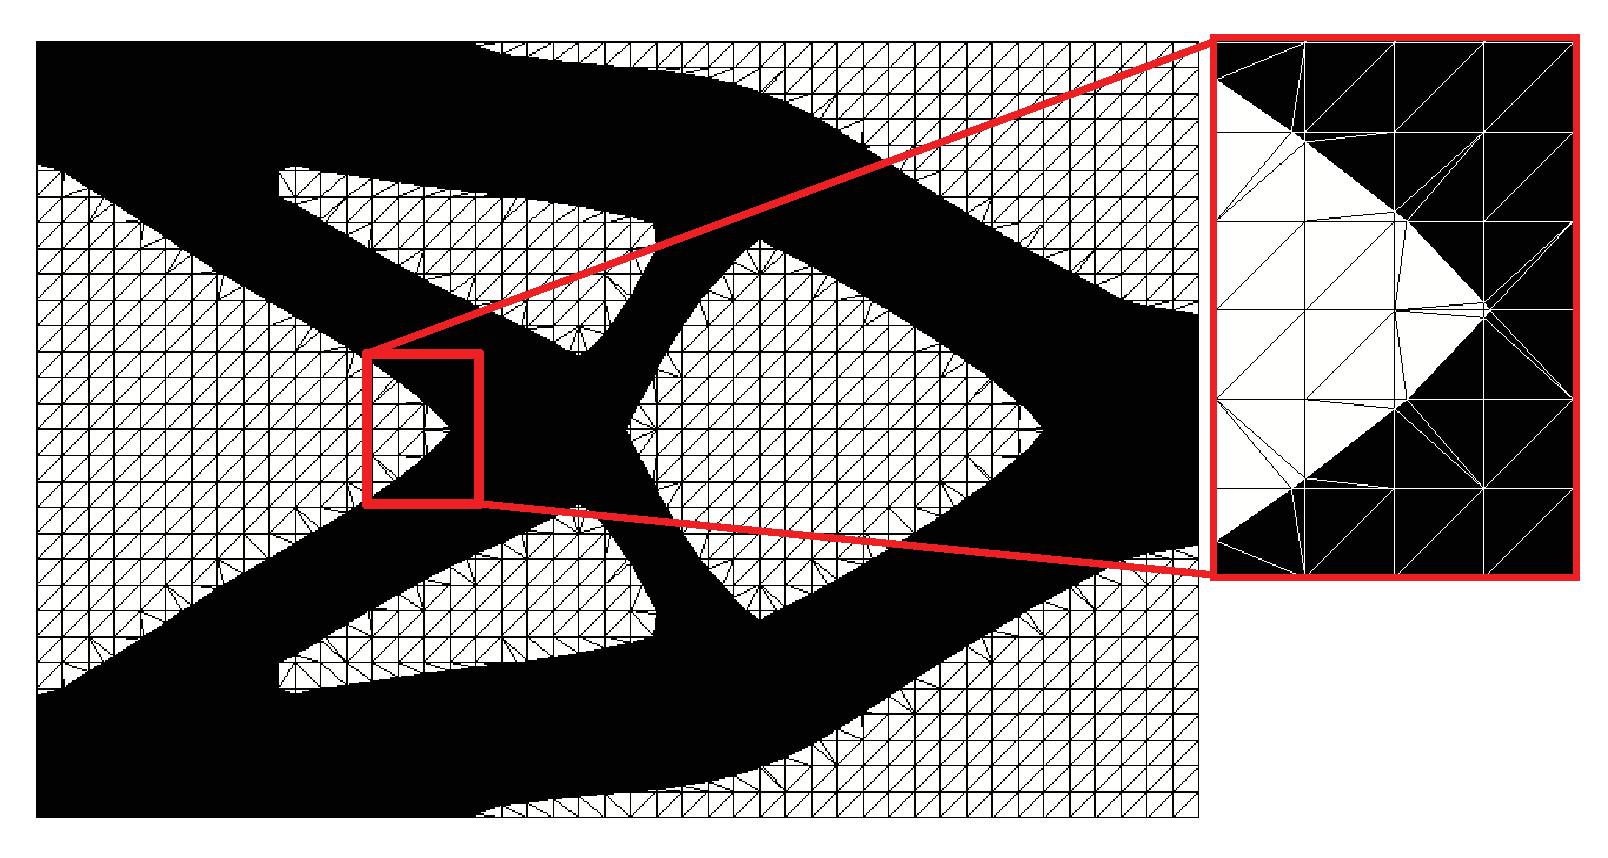
\includegraphics[scale=0.4]{structural_compliance_comparison_remeshing.eps}
	\caption{Remeshing the design domain such that elements align with the zero level set isolevel is an alternative to the Ersatz material interpolation approach.}
	\label{fig:remeshing_interpolation}
\end{figure}

Another approach is used by the XFEM (Section \ref{sec:intro_xfem}). The XFEM is an immersed boundary technique that works on fixed grids, and decomposes the cut elements into subdomains and interfaces that it uses for integration, as shown in Figure \ref{fig:XFEM_interpolation}.
%
\begin{figure}[H]
	\centering
	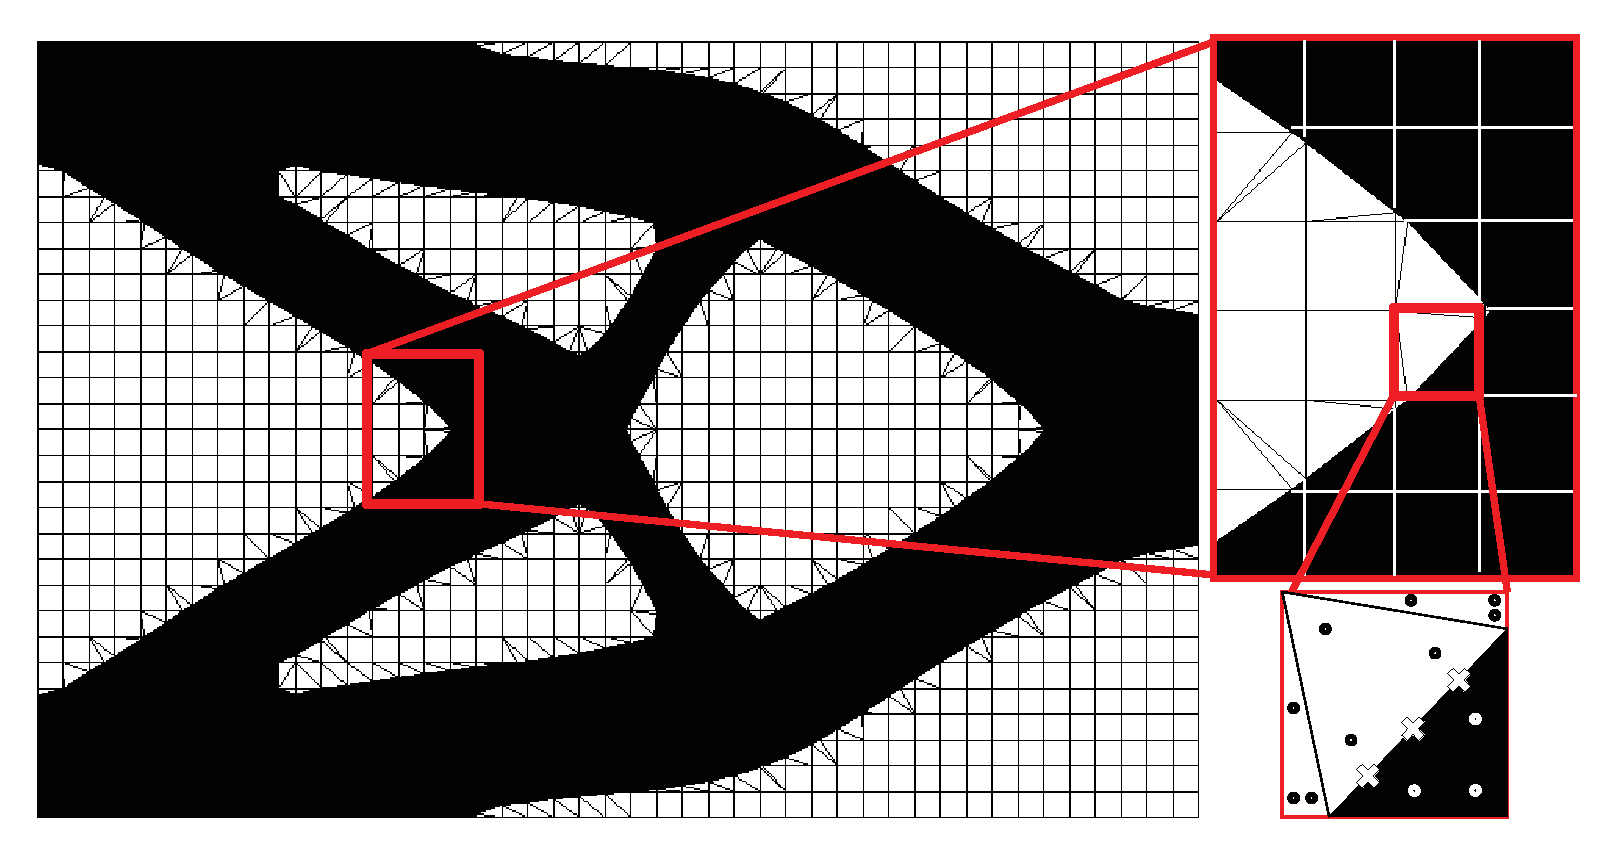
\includegraphics[scale=0.4]{XFEM_interpolation.eps}
	\caption{In the XFEM, the elements cut by the zero level set isolevel are divided into subdomains and interfaces for integration. Circles represent the abscissae for the subdomains, while crosses represent the abscissae for the interface integration.}
	\label{fig:XFEM_interpolation}
\end{figure}

The XFEM enriches the finite element solution space allowing for discontinuities (see Sections \ref{sec:discretization} and \ref{sec:computational-considerations} for details). In this thesis proposal, we will use a Heaviside enrichment strategy, which allows for solution fields with discontinuities $C^{-1}$.

As the topology of the level set function changes, it will occur that a phase subdomain is small enough to cause numerical instabilities in the system, and not lead to convergence. Several approaches have been studied in the literature to try and ameliorate this issue. \citep{LMD+:13} introduced a preconditioner that scales the solution space proportional to the areas of the subdomains. \citep{BH:12,SW:14,SRG+:14} used a ghost penalty formulation to smooth the gradients of the solution at the facets of the cut elements. Both approaches presented favorable results for two dimensional diffusion and incompressible Navier-Stokes flow problems.

Perimeter or curvature measures can be computed at the level set interface using the XFEM. These measures can be introduced into the optimization problem in order to provide a global shape control feature, and prevent the appearance of small floating particles \citep{MM:13}.

This thesis proposal will analyze the characteristics of the proposed LSM-XFEM method as follows:

\begin{enumerate}
	\item \citep{MM:13} studied the XFEM decomposition of the cut elements into subdomains, and the application of multiple enrichment levels in two dimensional problems. Our first hypothesis is that the same approach used by \citep{MM:13} can be extended to three dimensions. Section \ref{sec:a_complete_methodology_for_the_implementation_of_XFEM_inclusive_models} studies the algorithmic details of the approach, and the robustness of the method to describe complex three dimensional geometries using the level set method.

	\item The next question is whether the method can accurately describe the physics at the phase interface without extensive mesh refinement. If so, does it provide an advantage over the interface description provided by the density methods? There are several approaches to approximate the solution at the interface of the level set field, as described in Section \ref{sec:intro_xfem}. We will study the application of stabilized Lagrange multipliers in Section \ref{sec:density_and_level_set_XFEM_schemes_for_topology_optimization_of_3D_structures}, and of the Nitsche method in Section \ref{sec:level_set_XFEM_topology_optimization_of_3D_navier_stokes_and_scalar_transport_problems}.

	\item If the framework can describe complex geometries generated by a level set field, as well as accurately represent the physics at the phase interface, how does it fare overall against density approaches? Section \ref{sec:density_and_level_set_XFEM_schemes_for_topology_optimization_of_3D_structures} applies the framework to three dimensional structural problems, and provides a comprehensive comparison against density methods. The objective is to study convergence rates of the optimization problems, shape control of the optimized geometries, postprocessing capabilities of the methods to generate manufacturable designs, and the effects of providing different initial designs to the optimization process. The hypothesis is that the framework provides a better description of the geometry and material distribution than density methods, and therefore requires coarser meshes which leads to faster computations. Furthermore, it provides the capability to extract surface meshes directly from the level set function and manufacture the designs using three dimensional printing. This feature would be promising for rapid-prototyping.

	\item  In section \ref{sec:preconditioner}, we will expand the scaling preconditioning scheme to structural problems. The preconditioner was previously studied for two dimensional heat conduction problems. The scaling should ameliorate the effects that small intersection regions cause to the solution. In section \ref{sec:level_set_XFEM_topology_optimization_of_3D_navier_stokes_and_scalar_transport_problems}, we will study an alternate approach, the face-oriented ghost-penalty, and its effects on incompressible Navier-Stokes flows. This penalty formulation has been studied in the literature for diffusion and incompressible Navier-Stokes problems, and our hypothesis is that it can be applied in our optimization framework to ensure convergence for three dimensional problems.

	\item Once we can ensure convergence of the solution, the framework should be able to solve a broad range of design engineering problems. In this thesis proposal, we will study structural, incompressible Navier-Stokes flow, and scalar transport problems. These physics will help understand the characteristics, and the capability of the method to be applied to real-world engineering problems. Structural problems are studied in Section \ref{sec:density_and_level_set_XFEM_schemes_for_topology_optimization_of_3D_structures}. Incompressible Navier-Stokes and scalar transport problems are studied in \ref{sec:level_set_XFEM_topology_optimization_of_3D_navier_stokes_and_scalar_transport_problems}.

	\item Controlling the shape of the optimized geometry is important in manufacturing. The effects of using a smoothing filter for the level set field (see Section \ref{sec:intro_level_set_method}) will be studied in Section \ref{sec:feature-size-control}. This filter will also be compared against the density filter (see Section \ref{sec:smoothing_filter}) as a way of controlling the minimum feature size. Regularization techniques applied to the level set interface, such as measuring the curvature and perimeter, may cause different optimized geometries to emerge. The use of these measures and its effects on the finalized design will be studied in Section \ref{sec:topology_optimization_approaches_for_the_curvature_minimization_of_level_set_isocontours}.
\end{enumerate}

The studies proposed above will help us understand the characteristics and capabilities of the framework. The final step is to use this knowledge to study the method in the context of a real-world problem that requires the modeling of a three dimensional incompressible Navier-Stokes flow with a scalar transport field in Section \ref{sec:modeling_of_multiple_scalar_transport_fields_for_an_atomic_layer_deposition_machine}.

The specific objectives of this thesis proposal are then:
\begin{inparaenum}[(i)]
	\item To generate a robust LSM-XFEM topology optimization scheme;
	\item To compare the LSM-XFEM optimization scheme with traditional homogenization methods, such as SIMP, and study the advantages and disadvantages of our formulation;
	\item and to explore the characteristics of the methodology through cases studies in selected applications.
\end{inparaenum}

The layout of this thesis proposal is as follows: Section \ref{sec:introduction} presented the motivation and goals of the study, Section \ref{sec:background} presents an overview of the concepts required to understand this work, Section \ref{sec:a_complete_methodology_for_the_implementation_of_XFEM_inclusive_models} presents the algorithm to implement an XFEM framework in software, Section \ref{sec:density_and_level_set_XFEM_schemes_for_topology_optimization_of_3D_structures} presents the application of the methodology in structural problems, and compares the results to density approaches, Section \ref{sec:level_set_XFEM_topology_optimization_of_3D_navier_stokes_and_scalar_transport_problems} presents the application of the method to incompressible Navier-Stokes flows and scalar transport problems, Section \ref{sec:topology_optimization_approaches_for_the_curvature_minimization_of_level_set_isocontours} studies regularization techniques to improve the manufacturing of the design, Section \ref{sec:modeling_of_multiple_scalar_transport_fields_for_an_atomic_layer_deposition_machine} uses the methodology for a real-world design engineering problem. Finally, Sections \ref{sec:remaining_work} and \ref{sec:main_conclusions} show the remaining work and conclusions of this thesis proposal.

% -----------------------------------------------------------------------------

\chapter{Background}
\label{sec:background}

This chapter presents a brief overview on topology optimization, the level set method, and finite element methods. The information presented in this chapter is sufficient such that the reader can understand the framework in which the thesis is developed, but it is not comprehensive. References are provided for the reader who wishes to see more details on the topics.

% -----------------------------------------------------------------------------

\section{Optimization}
\label{sec:optimization}

An optimization problem is a problem in which you seek to find the best solution from the set of all feasible solutions. There are two categories of optimization problems, and their classification depends on whether the problem variables are continuous or discrete. In this work, we will focus on optimization problems with continuous variables. An optimization problem with discrete variables is known as a combinatorial optimization problem, and the reader is directed to \citep{NW:88} for a review.

The standard form for an optimization problem with continuous variables is:
%
\begin{equation}
\label{eq:optimization_standard_form}
	\begin{aligned}
		&\min_{\mathbf{s}} \mathcal{F}(\mathbf{s}, \mathbf{u}(\mathbf{s})), \\
		&\text{s.t.\,}
		\begin{cases}
			\mathbf{s}, & \text{subject to design constraints}  \ \mathcal{G}_j \leq 0 \text{,}\\
			\mathbf{u}, & \text{solves} \ W= 0 \ \text{for a given $\mathbf{s}$,}
		\end{cases}
	\end{aligned}
\end{equation}
%
where the goal is to minimize some objective functional $\mathcal{F}$ with respect to the vector of design variables $\mathbf{s}$. The design variables are subject to the $j$-th design constraint $\mathcal{G}_j$, which are enforced as an inequality problem. In general, the objective and constraints depend on the optimization variables, $\mathbf{s}$, and the state variables, $\mathbf{u}$. These state variables, $\mathbf{u}$, satisfy the weak form of the equilibrium equation $W$, which is enforced as an equality constraint. By convention, Equation \ref{eq:optimization_standard_form} defines a minimization problem. Maximization problems are handled by placing a negative sign on the objective functional $\mathcal{F}$.

% -----------------------------------------------------------------------------
% Optimization algorithms

There are several optimization algorithms available to update the design variables. For structural optimization problems with non-trivial and multiple constraints, the Method of Moving Asymptotes (MMA) \citep{Svanberg:87}, and its globally convergent counterpart, the Globally Convergent Method of Moving Asymptotes (GCMMA) \citep{Svanberg:02} have become the algorithms of choice. The work of this document will focus on the GCMMA algorithm. For a reference on more advanced mathematical tools, such as thr Sequential Quadratic Programming (SQP), the Sparse Nonlinear OPTimizer (SNOPT) \citep{GMS:02}, or the Interior Point OPTimizer \citep{WBL:06}, the reader is referred to the work of \citep{SM:13}.

% -----------------------------------------------------------------------------
% Design sensititivies

Gradients of the objective functional and design constraints with respect to the design variables are required by the mathematical algorithms specified above. The sensitivities for the optimization problems presented in this document will be computed using the adjoint method \citep{GP:08,YSL:02}.

In the following sections, we will delve into the approaches available to solve the optimization problem.

% -----------------------------------------------------------------------------

\section{Topology optimization}
\label{sec:intro_topology_optimization}

Topology optimization is a type of optimization problem in which you seek the optimal geometry and/or material layout of a body within a given design domain $D$. For example, mathematically we can formulate the following generic topology optimization problem: 
%
\begin{equation}
\label{eq:topology_optimization_generic}
		\min_{\mathbf{s}} \int_{\Omega} f \left( \mathbf{s(\mathbf{x})} \right) d{\Omega}
\end{equation}
%
which, analogous to Equation \ref{eq:optimization_standard_form} is subject to design constraints and equilibrium equations. The goal of the optimization problem is to minimize some objective functional $\int_{\Omega} f \left( \mathbf{s(\mathbf{x})} \right) d{\Omega}$ over the design domain with respect to the design variables $\mathbf{s(\mathbf{x})}$, where $\Omega$ represents the shape of the design. The optimization problem will set the design variables as ``on'' or ``off'' in order to minimize the design objective, while satisfying the design constraints. We can represent a design variable at a point $i$ as ``on'' by setting $s_{i}=1.0$, and ``off'' by $s_{i}=0.0$. A quick example is described in Figures \ref{fig:structural_compliance_setup} and \ref{fig:structural_compliance_example}. Figure \ref{fig:structural_compliance_setup} shows the setup for a topology optimization problem with an objective of minimal compliance and subject to a maximum volume fraction of $0.5$ for the solid phase. Figure \ref{fig:structural_compliance_example} shows the changes in the design, where the design variables at the elements are represented as ``on'' (black) or ``off'' (white) or in-between (grey).
%
\begin{figure}
	\centering
	\begin{tabularx}{\linewidth}{XX}
		\subfloat[Step 0.]{
			\label{fig:structural_compliance_0}
			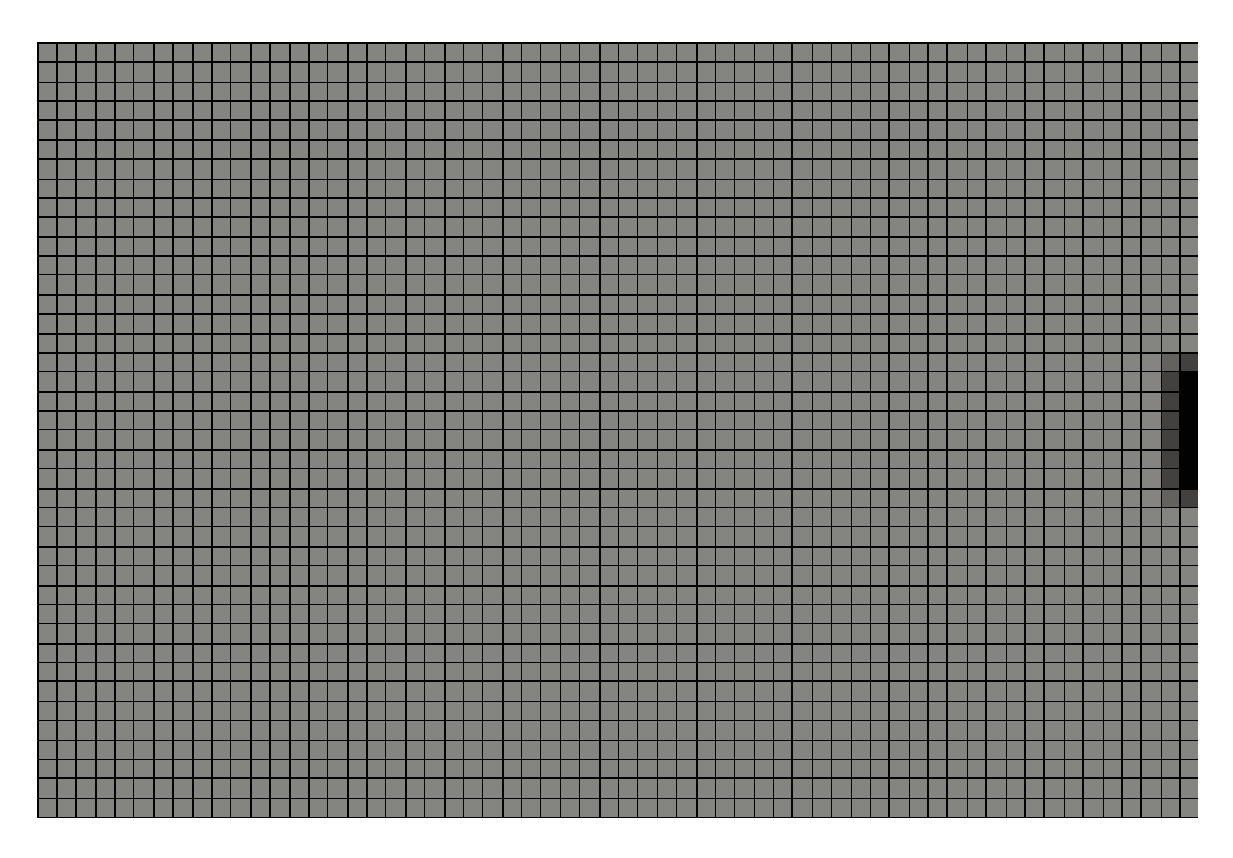
\includegraphics[width=\linewidth]{structural_compliance_0.eps}
		} &
		\subfloat[Step 5.]{
			\label{fig:structural_compliance_5}
			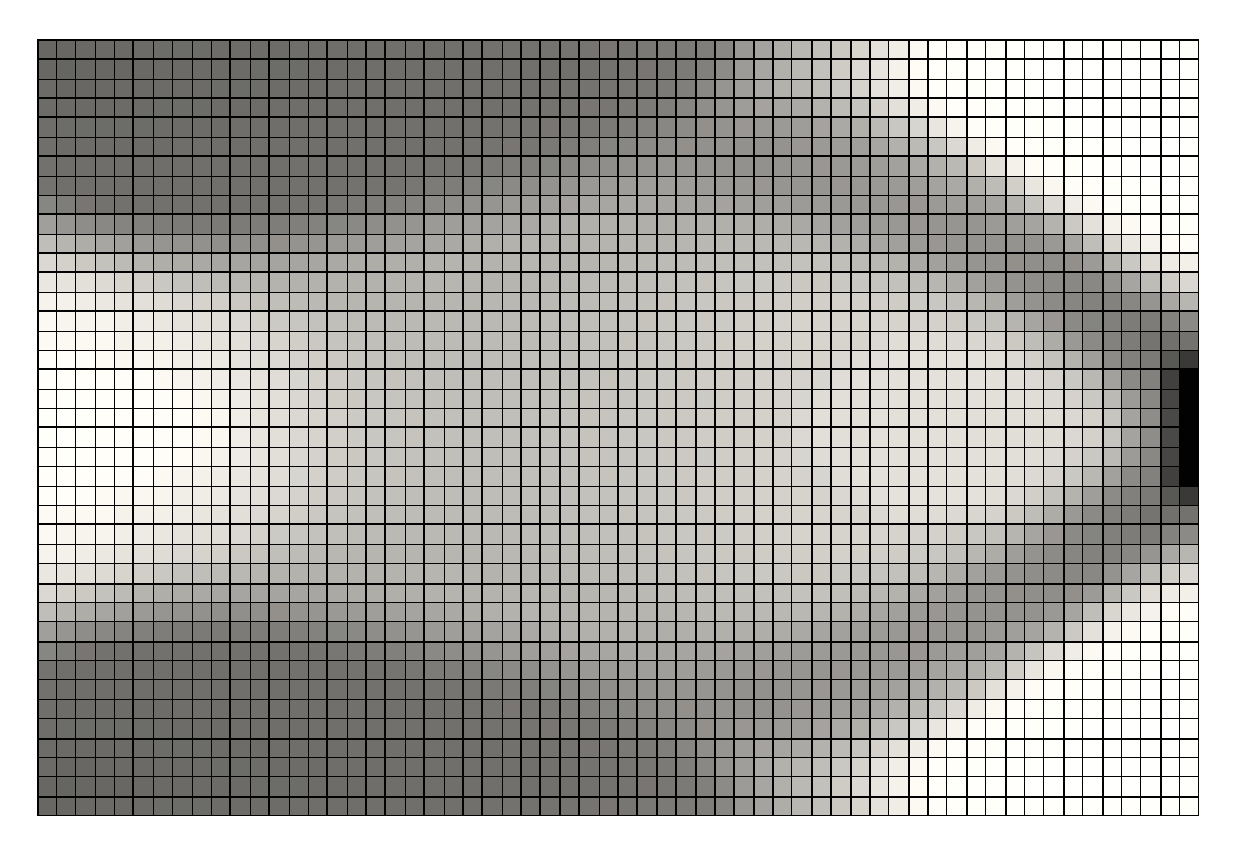
\includegraphics[width=\linewidth]{structural_compliance_5.eps}
		} \\
		\subfloat[Step 10.]{
			\label{fig:structural_compliance_10}
			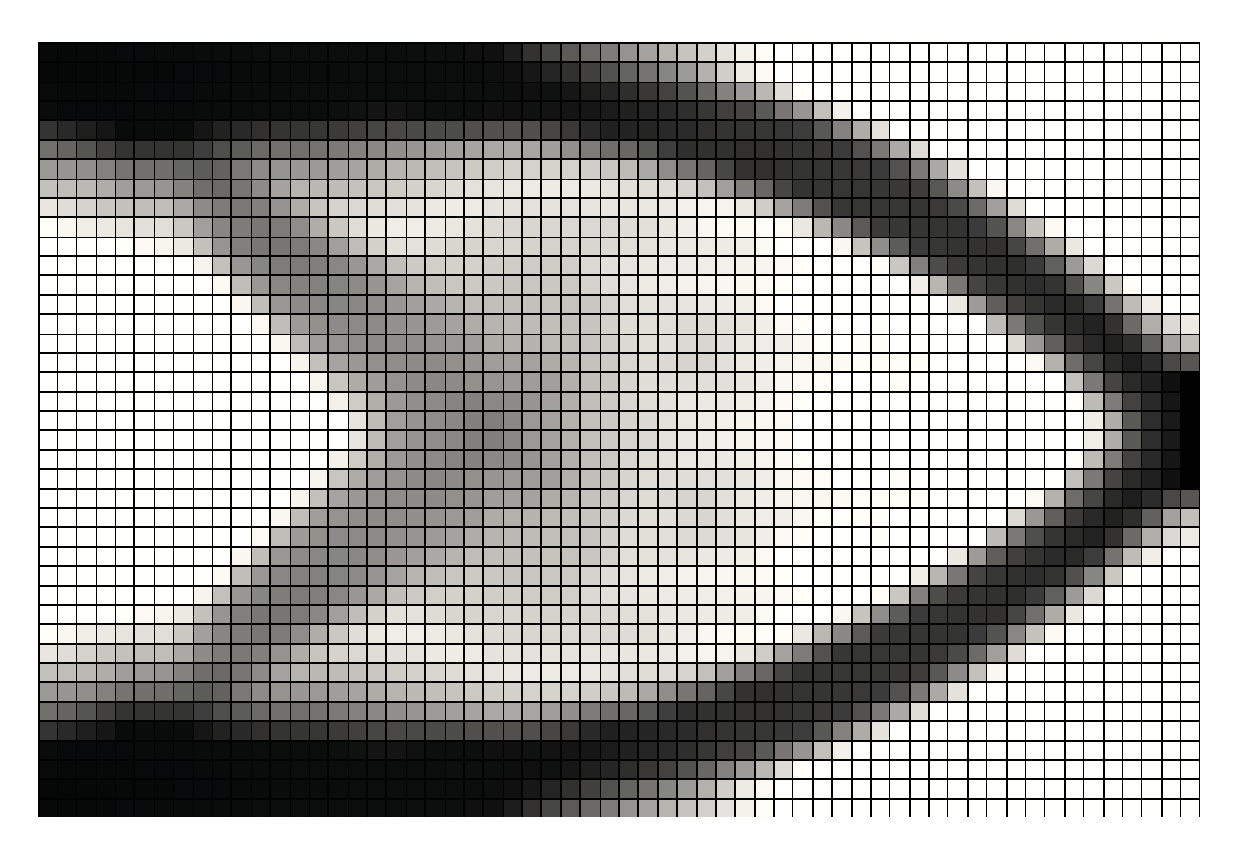
\includegraphics[width=\linewidth]{structural_compliance_10.eps}
		} &
		\subfloat[Step 15.]{
			\label{fig:structural_compliance_15}
			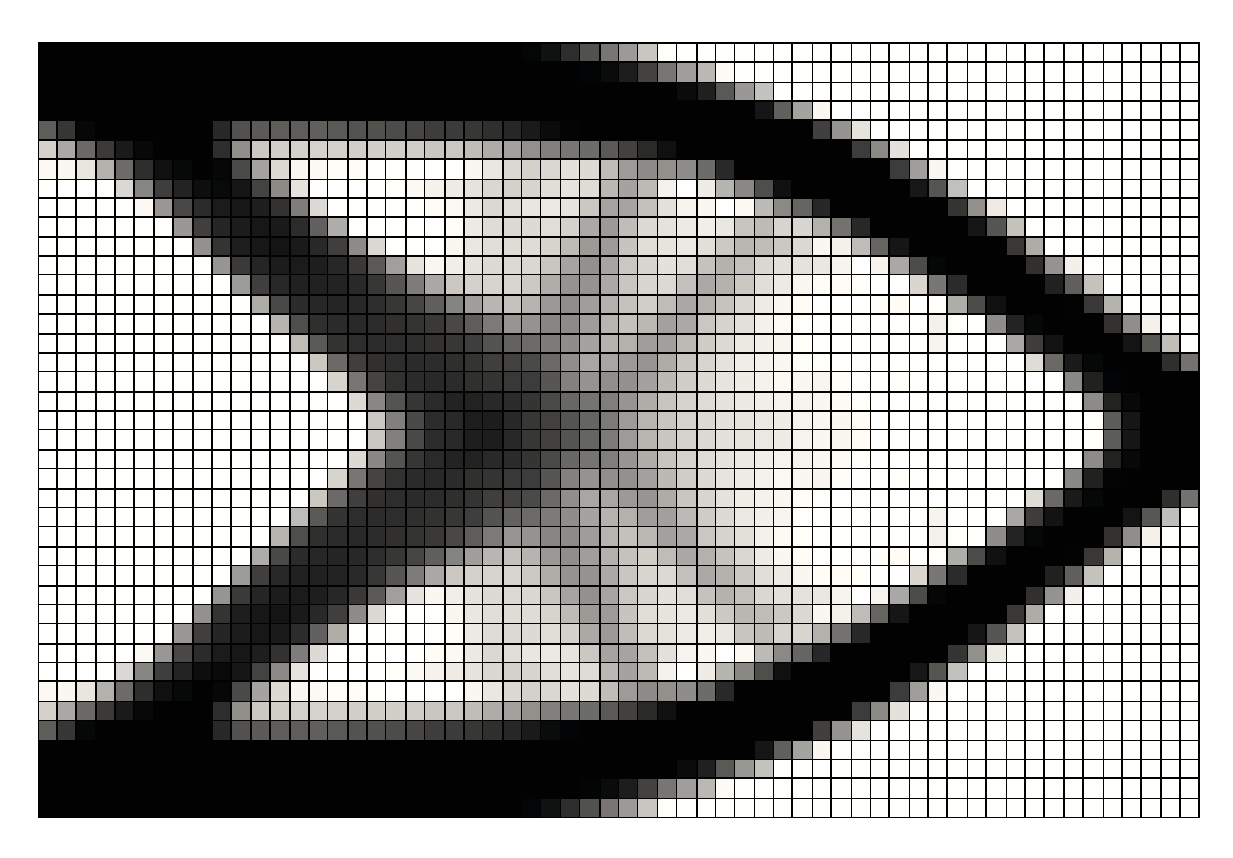
\includegraphics[width=\linewidth]{structural_compliance_15.eps}
		} \\
		\subfloat[Step 25.]{
			\label{fig:structural_compliance_25}
			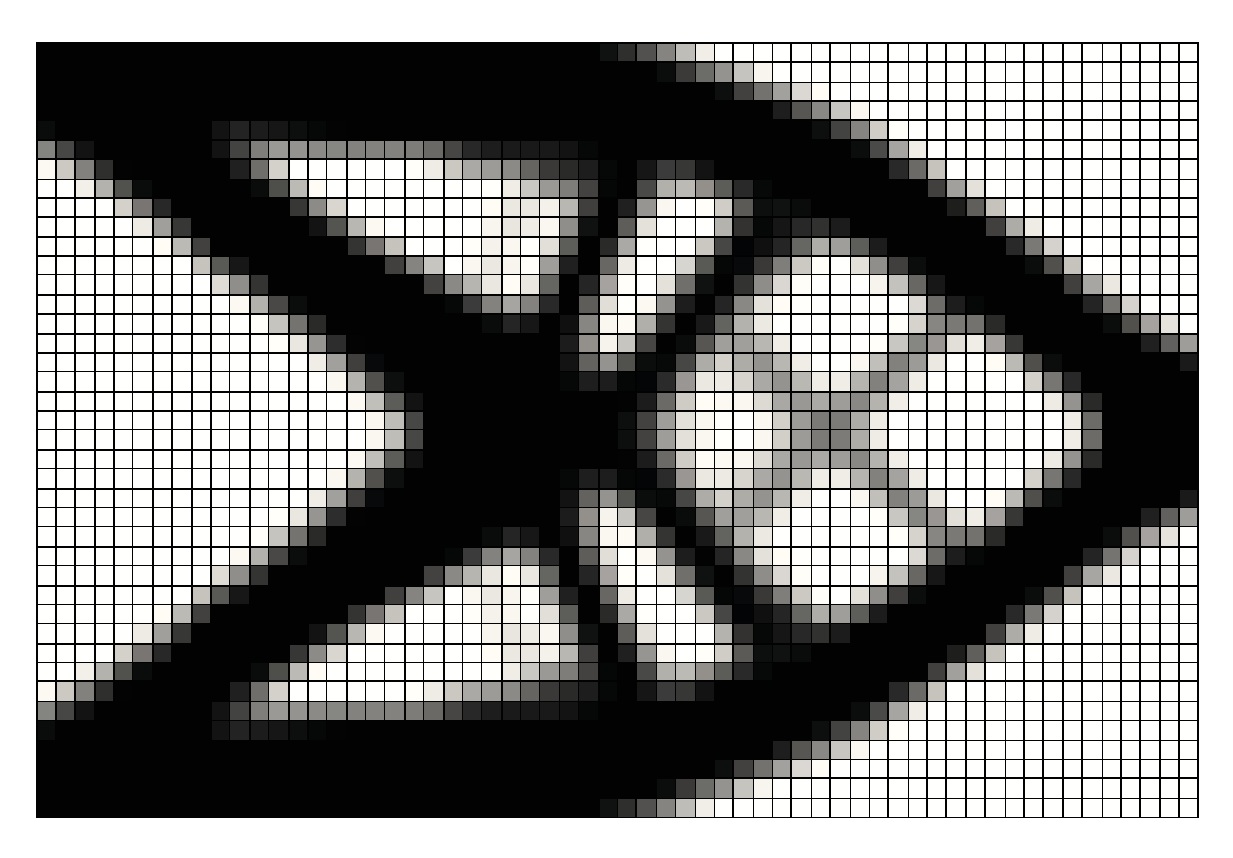
\includegraphics[width=\linewidth]{structural_compliance_25.eps}
		} &
		\subfloat[Step 50.]{
			\label{fig:structural_compliance_50}
			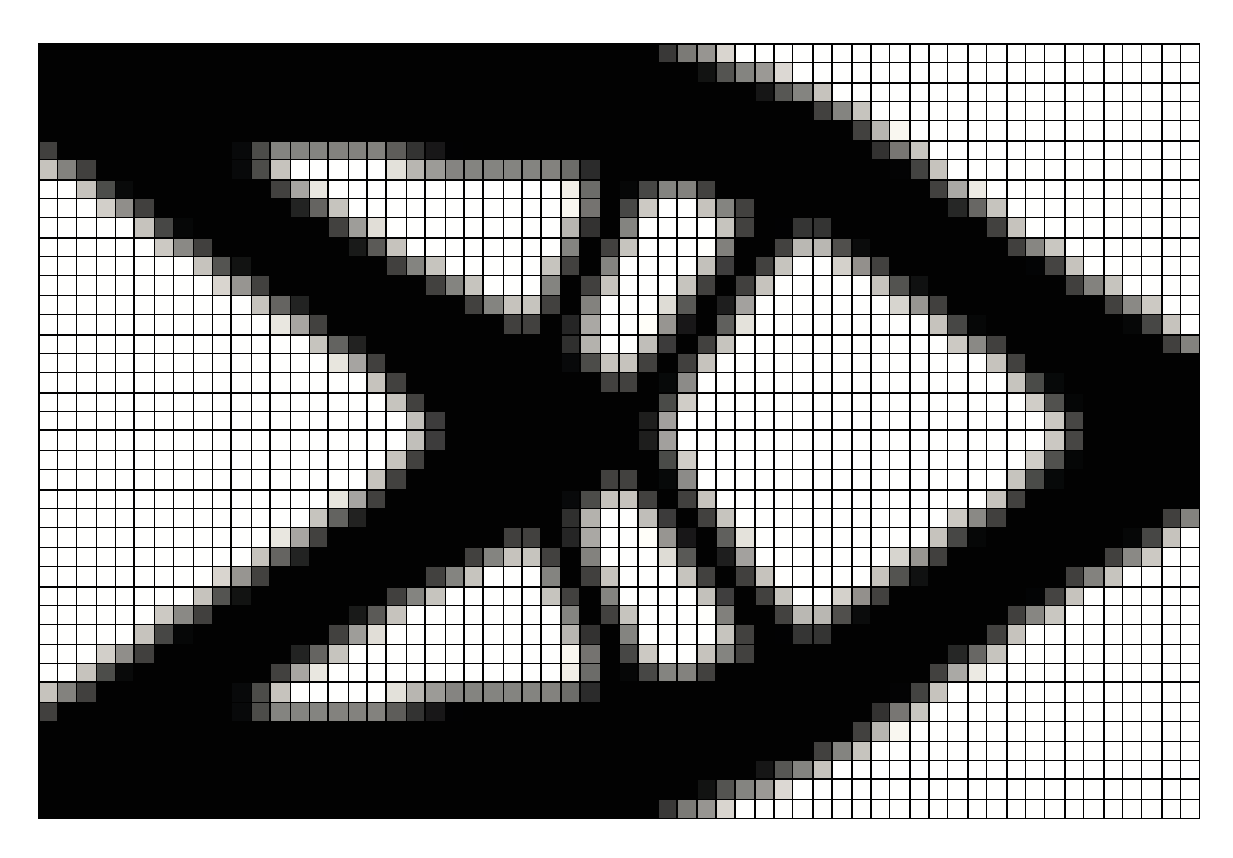
\includegraphics[width=\linewidth]{structural_compliance_50.eps}
		} \\
	\end{tabularx}
	\caption{Progression of the optimization process. Objective is to minimize compliance subject to a maximum volume fraction of 0.5 for the solid phase.}
	\label{fig:structural_compliance_example}
\end{figure}

Topology optimization provides the ability to create designs that are not always intuitive, or to improve on existing designs. Topology optimization methods were initially developed to create conceptual designs in the early stage of the design process \citep{BS:03,Rozvany:09}. It is interesting to note that the earliest recorded paper on topology optimization dates back to 1904, with the work of Australian inventor Michell in the derivation of optimality criteria for least-weight layout of trusses \citep{Michell:04}. And while topology optimization focused for decades on structural design, it has recently found its application in a wide range of physical disciplines \citep{BLO+:05} including acoustics \citep{FAN+:04}, wave propagation \citep{Frenzel:04}, electromagnetics \citep{LGD:09,SHW+:08} and optics \citep{BHF+:04,KOY:05}. For a more detailed review on topology optimization, please refer to \citep{BS:03,EO:01}.

% \footnote{\label{fn:topopt_app}
% At this point, the author recommends you take out your iPhone and iPad and download the best (and ahem... only) structural topology optimization application in the market, TopOpt, from the DTU Mechanical Engineering department. Use this as an exercise to reinforce the concepts explained in this paragraph. Start the application and define a structural problem adding boundary conditions and loads. Before you start the optimization process, try and think of what a good design would be for the problem at hand. Do this for several problems, and compare your intuition to the results of the optimization application. You may realize how helpful topology optimization can be for creating structures with the optimal design.}

% -----------------------------------------------------------------------------
% \subsection{Structural topology optimization}

Structural topology optimization, specifically topology optimization of continuum structures, is in its mathematical nature one of the most challenging optimization problems \citep{BS:03}. However, in 1988, \citep{BK:88} introduced their seminal paper on the homogenization method. In this method, the design domain is assumed to be formed by a material with micro-scale voids, and the topology optimization problem seeks the optimal porosity of the porous medium in order to minimize the objective functional. Due to its effectiveness and simplicity, homogenization-based methods found a lot of applications in structural design, and quickly became the main approach in structural topology optimization \citep{Bendsoe:89}. The homogenization method works by transforming the structural optimization problem into a standard nonlinear program where the design variables are coefficients of the underlying governing equation, and therefore is capable of producing internal holes in the design domain without \textit{a priori} knowledge of them.

% -----------------------------------------------------------------------------

\section{Density topology approaches}
\label{sec:density_topology_approaches}

In 1989, \citet{Bendsoe:89,ZR:91} introduced the most popular of homogenization methods, the ``solid isotropic material with penalization'' (SIMP). In SIMP, the design variables represent the artificial densities, $\rho\left(\mathbf{x}\right)$, of a group of elements in a fixed finite element grid (our design domain $D$) and their material properties are parameterized in terms of a set of material interpolation functions such that intermediate properties are penalized. The typical approach is to assume a value of $\rho=1.0$ represents solid material, while $\rho=0.0$ represents void.

% -----------------------------------------------------------------------------

\subsection{Smoothing filter}
\label{sec:smoothing_filter}

An additional numerical scheme is necessary to smear out numerical instabilities. This is referred to as the filtering method \citep{Sigmund:01a,Sigmund:01b}. For example, in structural topology optimization, the density, rather than being equal to a single variable, can be computed from a linear smoothing filter as follows:

\begin{equation}
	\label{eq:smoothing_filter_SIMP}
	\tilde{\rho}\left(\mathbf{s}\right)=\frac{\sum_{i=1}^{E}w_{i}s_{i}}{\sum_{i=1}^{E}w_{i}}
\end{equation}

with

\begin{equation}
	\label{eq:weight_SIMP}
	w_{i}=\max \left( 0, r_{\rho} - \Vert \mathbf{x}_i - \mathbf{x} \Vert \right)
\end{equation}

where $s_{i}$ is equivalent to an artificial density $\rho$ at a point $\mathbf{x}_{i}$, $\mathbf{x}_{i}$ is the location of the node at which the design variable $i$ is defined, $\tilde{\rho}\left(\mathbf{s}\right)$ is the density at a point $\mathbf{x}$,  $w_{i}$ is the factor of point $\mathbf{x}$ with respect to the design variable $i$, $r_{\rho}$ is the filter radius, and $E$ is the number of elements in the design domain.

The filter in Equation \ref{eq:smoothing_filter_SIMP} prevents the formation of features smaller than $r_{\rho}$, and serves as a minimum feature size control. However, this comes at the cost of forming intermediate densities along the material interface. Methods for smearing out intermediate densities have been proposed by \citep{FJP:05,Sigmund:07,SS:01a}. \citep{GPB:04} proposed a density projection method to reduce the volume occupied by material with intermediate densities. This projection is based on a smoothed Heaviside function and applied to the densities as follows:
%
\begin{equation}
\label{eq:heaviside_density}
		\hat{\rho}\left(\tilde{\rho}\right) = 1-e^{-\beta\tilde{\rho}}+\tilde{\rho}e^{-\beta}
\end{equation}
%
where $\hat{\rho}$ is the projected density, and the parameter $\beta \ge 0$ controls the crispness of the projection. Notice that for $\beta=0$ we recover the original density $\hat{\rho}=\tilde{\rho}$. As we increase $\beta$, more and more intermediate densities are penalized towards the value of 1.0, as shown in Figure \ref{fig:density_heaviside}. Note, however, that if the objective and/or constraints of the optimization problem find the intermediate densities to be benefitial, the optimization algorithm will ignore the effects of this projection scheme. The reader is referred to \citep{GPB:04,GAH:11,Sigmund:07,XCC:10,WLS:11} for more details on projection schemes.
%
\begin{figure}
	\centering
	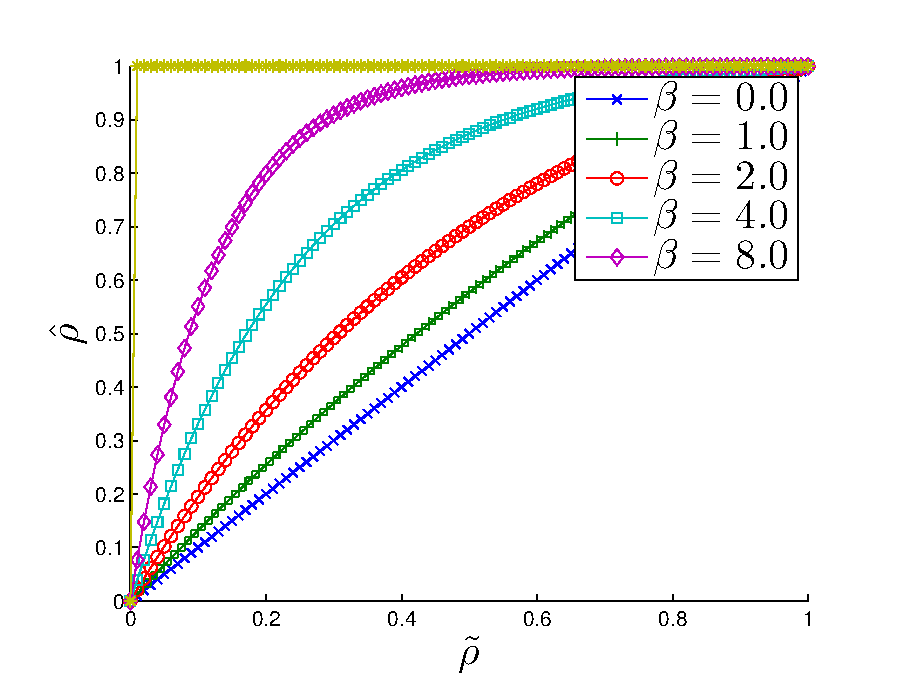
\includegraphics[scale=0.75]{density_heaviside.eps}
	\caption{The density Heaviside projection for various magnitudes of $\beta$.}
	\label{fig:density_heaviside}
\end{figure}
%
In structural topology optimization, it is important to model the relation between density and stiffness. SIMP models the stiffness proportional to the density in the power $p$, where $p > 1$ \citep{BS:99}, in order to guarantee a well-posed optimization problem \citep{BS:99}. The structural stiffness for a ``solid-void'' problem can then be formulated as:
%
\begin{equation}
\label{eq:structural_stiffness}
		E\left(\mathbf{x}\right) = \hat{\rho} ^ p E_{0}
\end{equation}
%
where $E_{0}$ is the initial structural stiffness of the material. Typically, the parameter $p$ is set to 1, and then increased as the optimization progresses \citep{RZS:94}; this is the so-called continuation method \citep{SP:98}. It was shown that if one uses $p > 3$, we recover a black-and-white binary-like material distribution \citep{BS:03}. That is why the density approach has been referred to as a \textit{pixelated} geometric model.

% -----------------------------------------------------------------------------
% Multimaterial SIMP
% \subsection{Multimaterial SIMP}

The SIMP method can be expanded to model a multi-material optimization problem. For example, applying a ``rule of mixture'', we can model a two-phase material in structural topology optimization by modifying Equation \ref{eq:structural_stiffness} as:

\begin{equation}
	\label{eq:two_phase_stiffness}
	E\left(x\right) = \hat{\rho} ^ p E_{A} + \left( 1 - \hat{\rho} ^ p \right) E_{B}
\end{equation}

where $E_{A}$ represents the stiffness of material ``A'', and $E_{B}$ represents the stiffness of material ``B''. Notice that if we model the material phase ``B'' as void, and set $E_{B}=0$ we recover the original equation from \ref{eq:structural_stiffness}. This method uses a single design variable field to model up to two different materials.

For a three-phase or more material optimization problem, we require an extended power law interpolation with multiple design variable fields (i.e. $\mathbf{s}_{1}$, $\mathbf{s}_{2}$, etc.), as shown in \citep{WW:04c,PS:14}. In general, the SIMP method requires $\left( n - 1 \right)$ design variable fields for $n$ distinct material phases \citep{WW:04c}.

% -----------------------------------------------------------------------------

\subsection{Density methods applied to fluid dynamics}
\label{sec:intro_density_fluid_dynamics}

Several applications require finding the optimal geometries of systems to improve the performance of internal and external flows \citep{Maute:14}. Adopting the concept of density methods, \citep{BP:03} extended the methodology to fluid related problems. They modeled the influence of a wall or body in the fluid flow by representing it as a body force in the incompressible Navier-Stokes equations as:
%
\begin{equation}
	\label{eq:navier_stokes}
	\rho^{f} \left( \frac{\partial v_{i}}{\partial t} + v_{j} \frac{\partial v_{i}}{\partial x_{j}} \right) = \frac{\partial}{\partial x_{j}} \left( -p \delta_{ij} + \mu^{f} \left( \frac{\partial v_{j}}{\partial x_{i}} + \frac{\partial v_{i}}{\partial x_{j}} \right) \right) + f_{i}
\end{equation}
%
\begin{equation}
	\label{eq:divergence_stokes}
	\frac{\partial v_{i}}{\partial x_{i}} = 0
\end{equation}
%
where $\rho^{f}$ is the fluid density, $v_{i}$ is the velocity along the spatial dimension $i$, $p$ is the fluid mechanical pressure, $\mu^{f}$ is the fluid dynamic viscosity, and $f_{i}$ is the force exerted by the porous media:
%
\begin{equation}
	\label{eq:brinkman_force}
	f_{i} = - \alpha v_{i}
\end{equation}
%
This methodology is referred to as the Brinkman penalization. Similar to structural topology optimization problems, we set the design variables, $\mathbf{s}$, to represent the fluid fraction at a point of the design domain, and set $\mathbf{s}=\gamma=\gamma \left( \mathbf{x} \right)$, where $\left( 0 \le \gamma \le 1 \right)$. Typically, $\gamma = 1$ represents the fluid domain, and $\gamma=0$ represents the solid domain.

The coefficient $\alpha$ can be interpolated from the design variables as:
%
\begin{equation}
	\label{eq:alpha_linear}
	\alpha = \alpha_{max} \gamma
\end{equation}
%
The parameter $\alpha_{max}$ should be large enough such that the term $\mathbf{f}$ in Equation \ref{eq:navier_stokes} sufficiently penalizes the flow to $\mathbf{u}=0$. \citep{KMK:12} set $\alpha_{max}$ to:
%
\begin{equation}
	\label{eq:alpha_max}
	\alpha_{max} = \left( 1 + \frac{1}{Re} \right) \chi
\end{equation}
%
where $Re$ is the Reynolds number, and $\chi$ is set to a very large value, i.e. $10^4$.

However, this linear interpolation causes large gradients in the fluid flow, which cause numerical issues and may lead to the optimization problem converging to a local minimum. \citep{BP:03} introduced a convex interpolation:
%
\begin{equation}
	\label{eq:alpha_interpolation}
	\alpha \left( \mathbf{x} \right) = \alpha \left( \gamma \left( \mathbf{x} \right) \right) = \alpha_{max} + \gamma \left( \alpha_{min} - \alpha_{max} \right) \frac{1 + \alpha_{p}}{\gamma + \alpha_{p}}
\end{equation}
%
Figure \ref{fig:alpha_convex} shows the influence of the perimeter $\alpha_{p}$. In general, we want to choose $\alpha_{p}$ to be as low as possible, but high enough to prevent intermediate porosities from showing up in the optimization process. In the work of \citep{KM:11}, $\alpha_{p}$ was chosen to be 0.01 with favorable results. $\alpha_{min}$ is set to zero, such that at its minimum, $\alpha=0$ recovers the original Navier-Stokes equations.
%
\begin{figure}
	\centering
	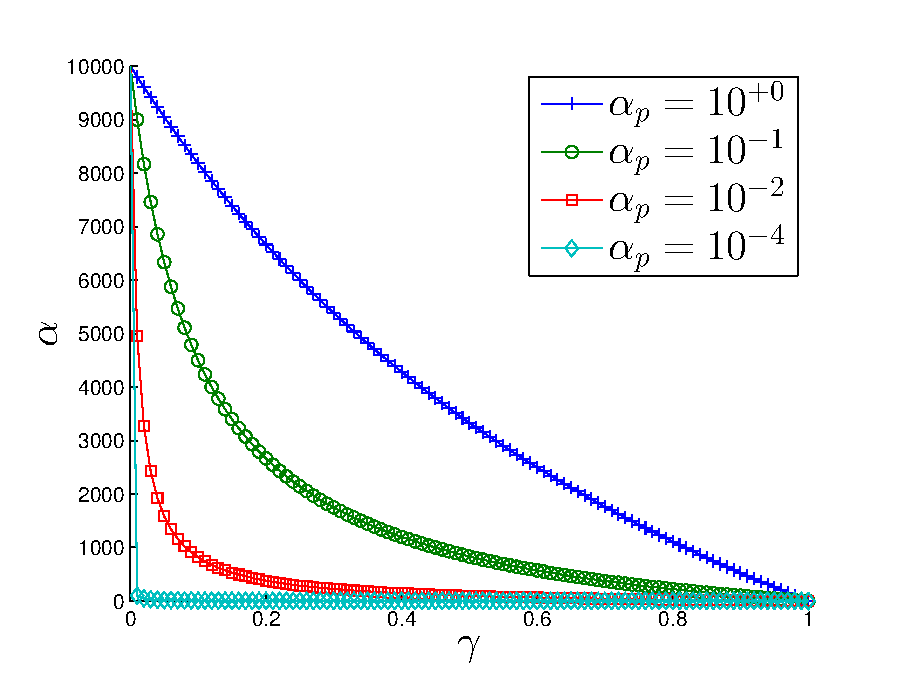
\includegraphics[scale=0.75]{alpha_convex.eps}
	\caption{Influence of the interpolation penalty $\alpha_{p}$.}
	\label{fig:alpha_convex}
\end{figure}
%
For more details on topology optimization of Stokes and Navier-Stokes flows, the reader is referred to \citep{Maute:14}.

% -----------------------------------------------------------------------------

\subsection{Discussion of the SIMP approach}
\label{sec:SIMP_discussion}

The concept of relating some artificial densities to the stiffness in structural problems can be expanded to other physics disciplines. The SIMP method can be used the describe material properties in thermal conductivity, magnetic permeability, porosity, etc.; and therefore, it found its way to a wide range of applications. The method requires a relatively small amount of iterations in order for the optimization problem to converge to an optimal design (at least for ``solid-void'' problems). SIMP has this capability because it operates on the entire design domain and not only on the boundaries; therefore, it does not suffer from localization effects. The approach is also suitable for a wide combination of design constraints, multiple load conditions, and extremely large (often 3D) systems. The educational article by \citet{Sigmund:01b} detailing a 99-line SIMP-code implemented in Matlab, as well as his web-based topology optimization program \citep{TS:01}\footnote{The software is now available on iOS phones and tablets.} played an important role in the acceptance of the SIMP method in both the academic and industry communities. Virtually all industrial optimization software uses the SIMP method as their optimization method of choice due to its ease of implementation.

% -----------------------------------------------------------------------------
% What are the disadvantages?

The SIMP method typically describes the interface between the different material domains either by using intermediate densities or by discrete material distributions, which may lead to jagged boundaries. In both cases, the representation of the interface is not precise, and therefore, the enforcement of boundary conditions at the interface is hindered. This may result in non-physical responses, such as premature yielding \citep{MSR:98} in structural mechanics, fluid flow penetrating solid material in low Reynolds number flow \citep{KPM:11}, and scalar fields diffusing through solid material at low P\'{e}clet number flow \citep{MPY+:12}. This issue can be mitigated by representing the material interface more accurately either by mesh refinement or adaptive re-meshing \citep{MR:95,MR:97}. However, for problems that require an accurate geometrical description of the interface, such as stresses in elasticity, boundary layer problems in fluids and skin-depth issues in electromagnetics, SIMP (and other material interpolation methods) will fail due to the jagged edges obscuring the physics \citep{ES:11,YNK+:11}.

Using material interpolation to address multi-material optimization problems is not a physics-based technique, and has been shown to violate the Hashin-Shtrikman bounds for low values of $\rho$ and large values of $p$ \citep{HS:62}. Furthermore, modeling multiple material phases can become complicated \citep{YA:01} and lead to slow convergence due to the larger number of iterations, as shown in \citep{VM:14}.

% -----------------------------------------------------------------------------
% Level set method

\section{Level set method}
\label{sec:intro_level_set_method}

The level set method applied to topology optimization arose as a technique capable of overcoming some of the shortcomings of the density approach. The main advantage of the method is that it allows for the description of complex geometries and the variation of the shape and topology of our design without introducing intermediate materials. A level set approach is a \textit{region-based} model with explicit boundaries, in contrast to the \textit{pixelated} model of the density method \citep{WW:04c}.

The level set method was first used to implicitly represent a structural boundary by \citep{OS:88}. Since then, it has been applied extensively in the field of imaging and computer visions \citep{OP:03}. The level set method eventually found its way to topology optimization, as the technique is well suited for the task: level set functions can form holes, split into multiple pieces, or merge with other level set functions \citep{WW:04c,AJT:02,OS:88}. 

The basic idea behind using the level set method to represent a shape boundary $\Gamma = \partial \Omega$ is to express a curve or surface as the zero level set of a higher dimensional implicit function $\phi$, as shown in Figures \ref{fig:level_set_circle_func_025}, \ref{fig:level_set_circle_func_050}, and \ref{fig:level_set_circle_func_075}, such that:
%
\begin{equation}
	\centering
	\label{eq:isolevel}
	\Gamma = \lbrace \mathbf{x} : \phi\left(\mathbf{x}\right) = 0 \rbrace
\end{equation}
%
Then we can divide the design domain into phase regions as:
%
\begin{equation}
	\centering
	\label{eq:level_set_regions}
	\begin{split}
		\phi\left(\mathbf{x}\right) > 0 & \quad \forall \mathbf{x} \in \Omega \backslash \partial \Omega \text{ (inside the region)} \\
		\phi\left(\mathbf{x}\right) = 0 & \quad \forall \mathbf{x} \in \partial \Omega \text{ (on the boundary)} \\
		\phi\left(\mathbf{x}\right) < 0 & \quad \forall \mathbf{x} \in D \backslash \Omega \text{ (outside the region)}
	\end{split}
\end{equation}
%
where $D$ represents the design domain, either bounded or unbounded, and contains all possible admissible shapes of $\Omega$, as shown in Figures \ref{fig:level_set_circle_domain_025}, \ref{fig:level_set_circle_domain_050}, and \ref{fig:level_set_circle_domain_075}. Each phase region may represent a different material \citep{AJT:02,WW:04c,OS:01,SW:00} or a different physics \citep{LCB:06,GW:08}. In the work of this thesis, the level set method is discretized with a finite element mesh.
%
\begin{figure}
	\centering
	\begin{tabularx}{\linewidth}{XX}
		\subfloat[]{
			\label{fig:level_set_circle_domain_025}
			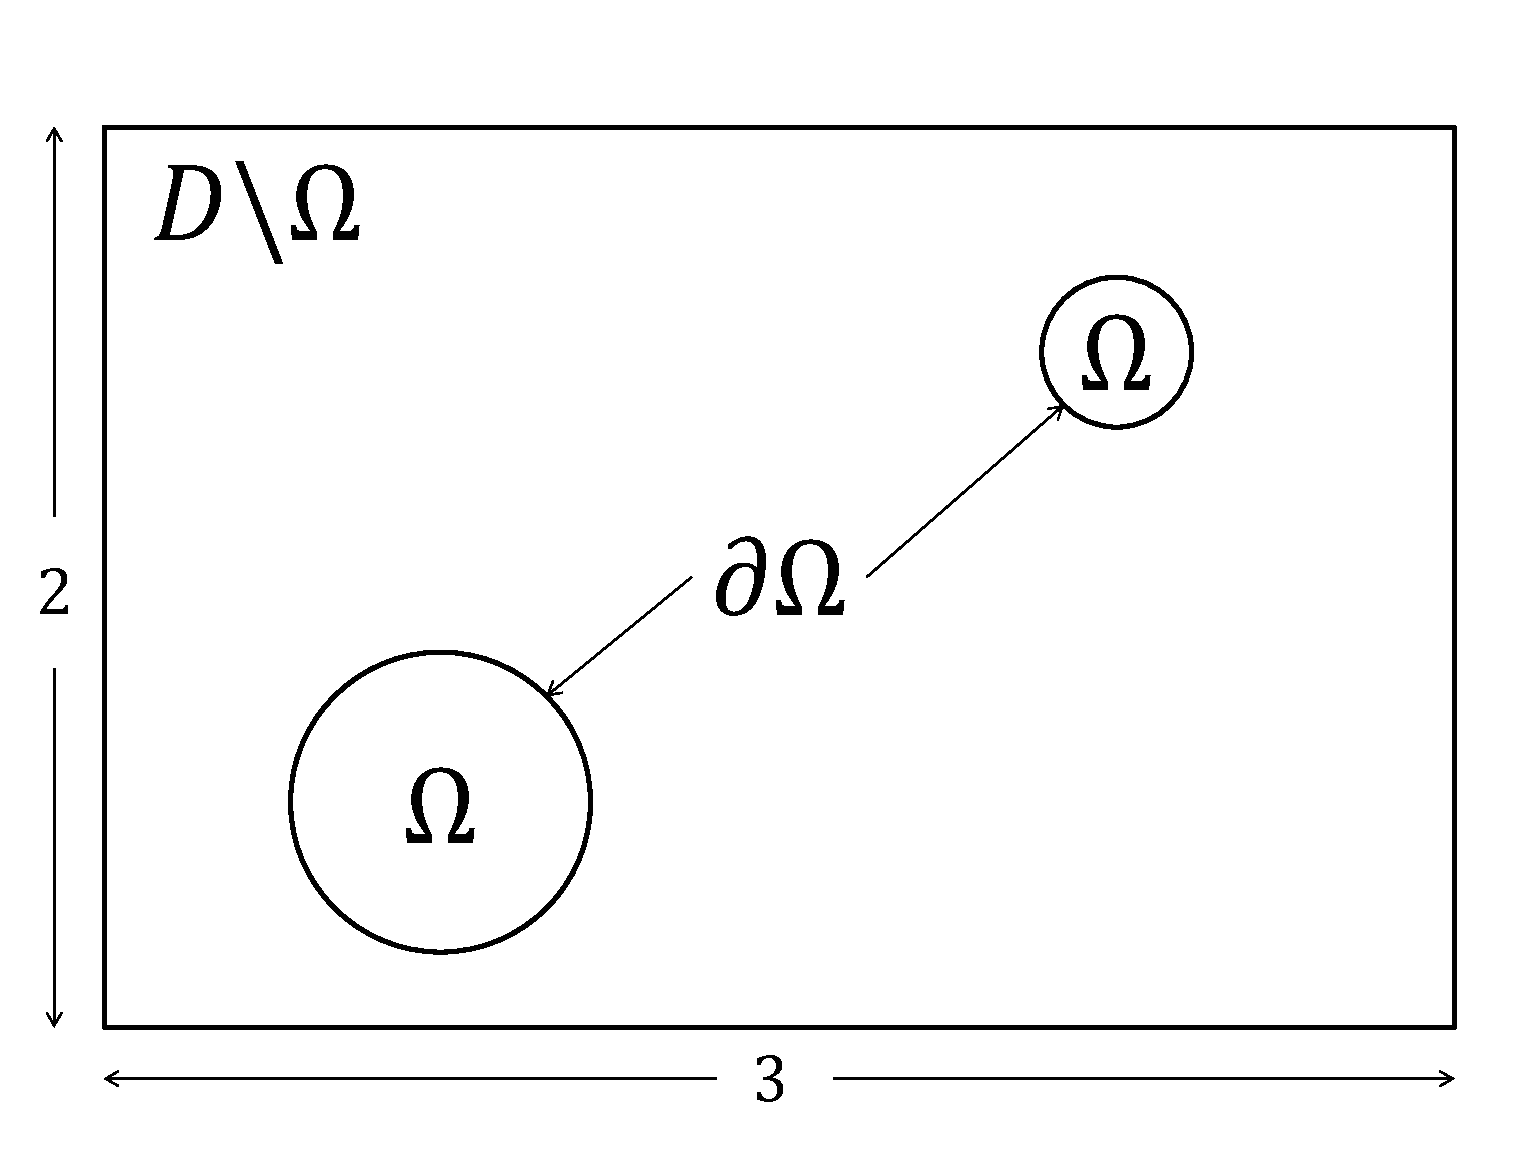
\includegraphics[width=\linewidth]{level_set_circles_1.eps}
		} &
		\subfloat[]{
			\label{fig:level_set_circle_func_025}
			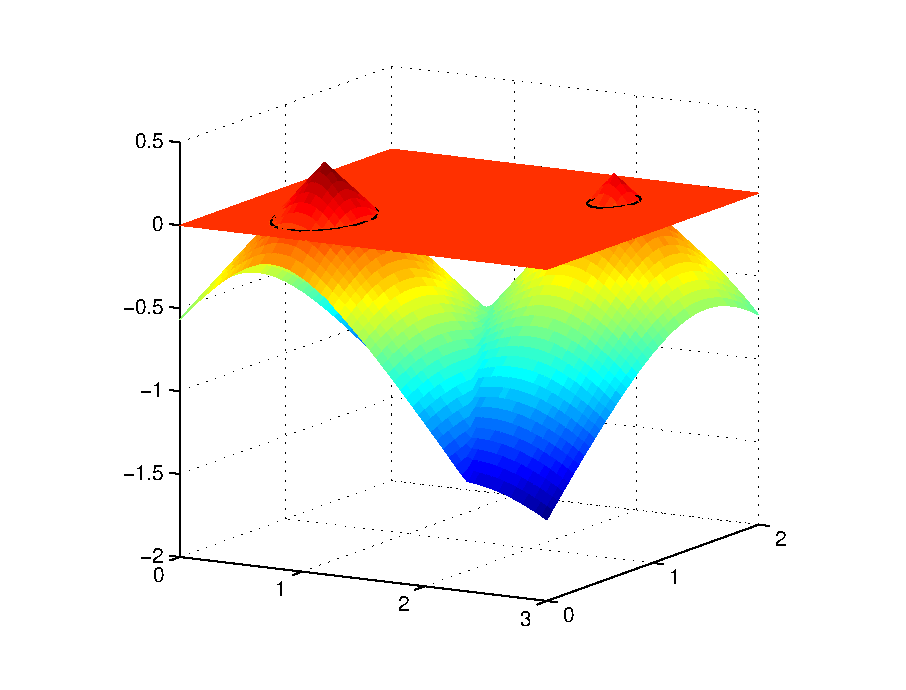
\includegraphics[width=\linewidth]{level_set_function_circles_1.eps}
		} \\
		\subfloat[]{
			\label{fig:level_set_circle_domain_050}
			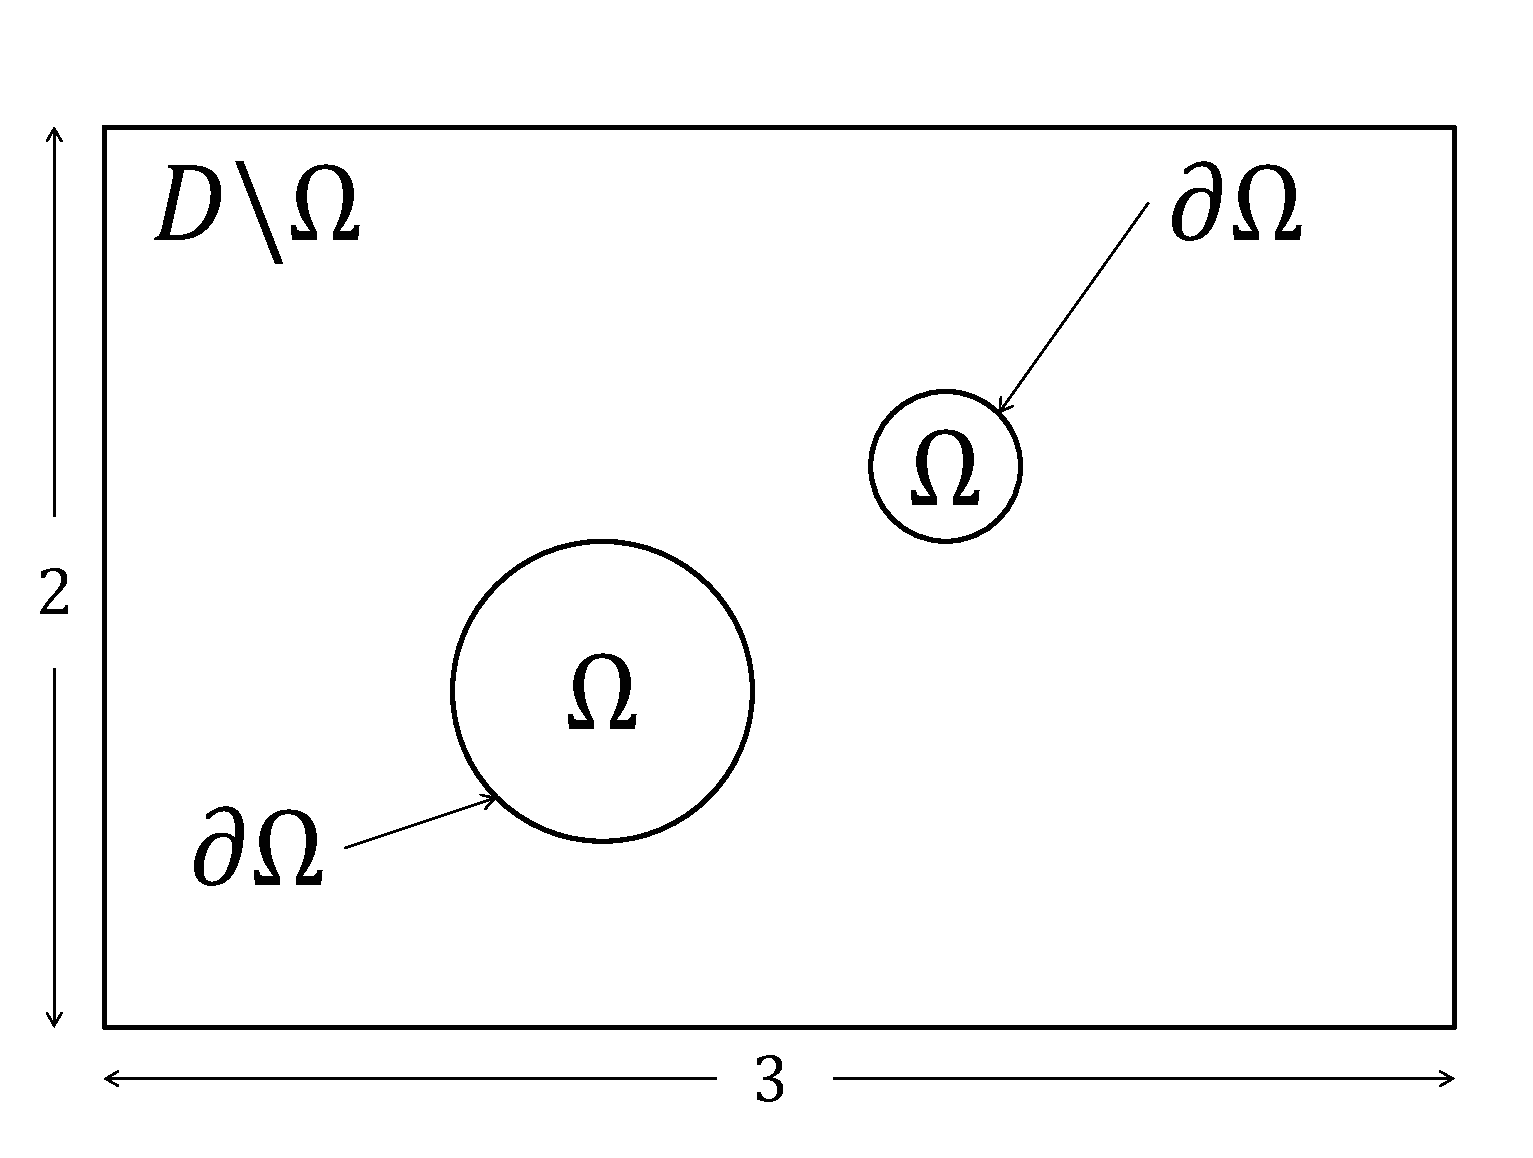
\includegraphics[width=\linewidth]{level_set_circles_2.eps}
		} &
		\subfloat[]{
			\label{fig:level_set_circle_func_050}
			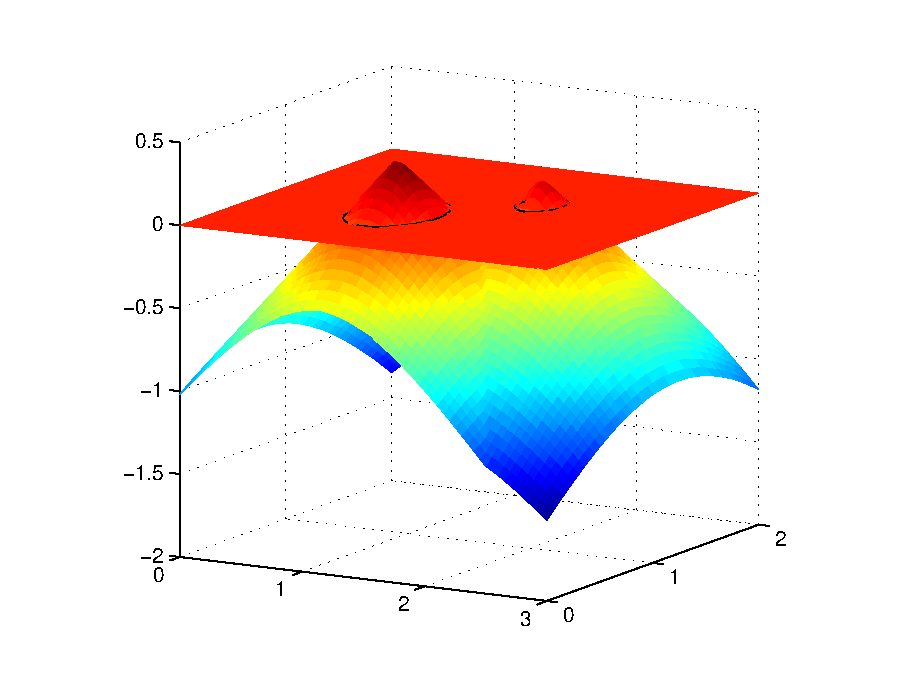
\includegraphics[width=\linewidth]{level_set_function_circles_2.eps}
		} \\
		\subfloat[]{
			\label{fig:level_set_circle_domain_075}
			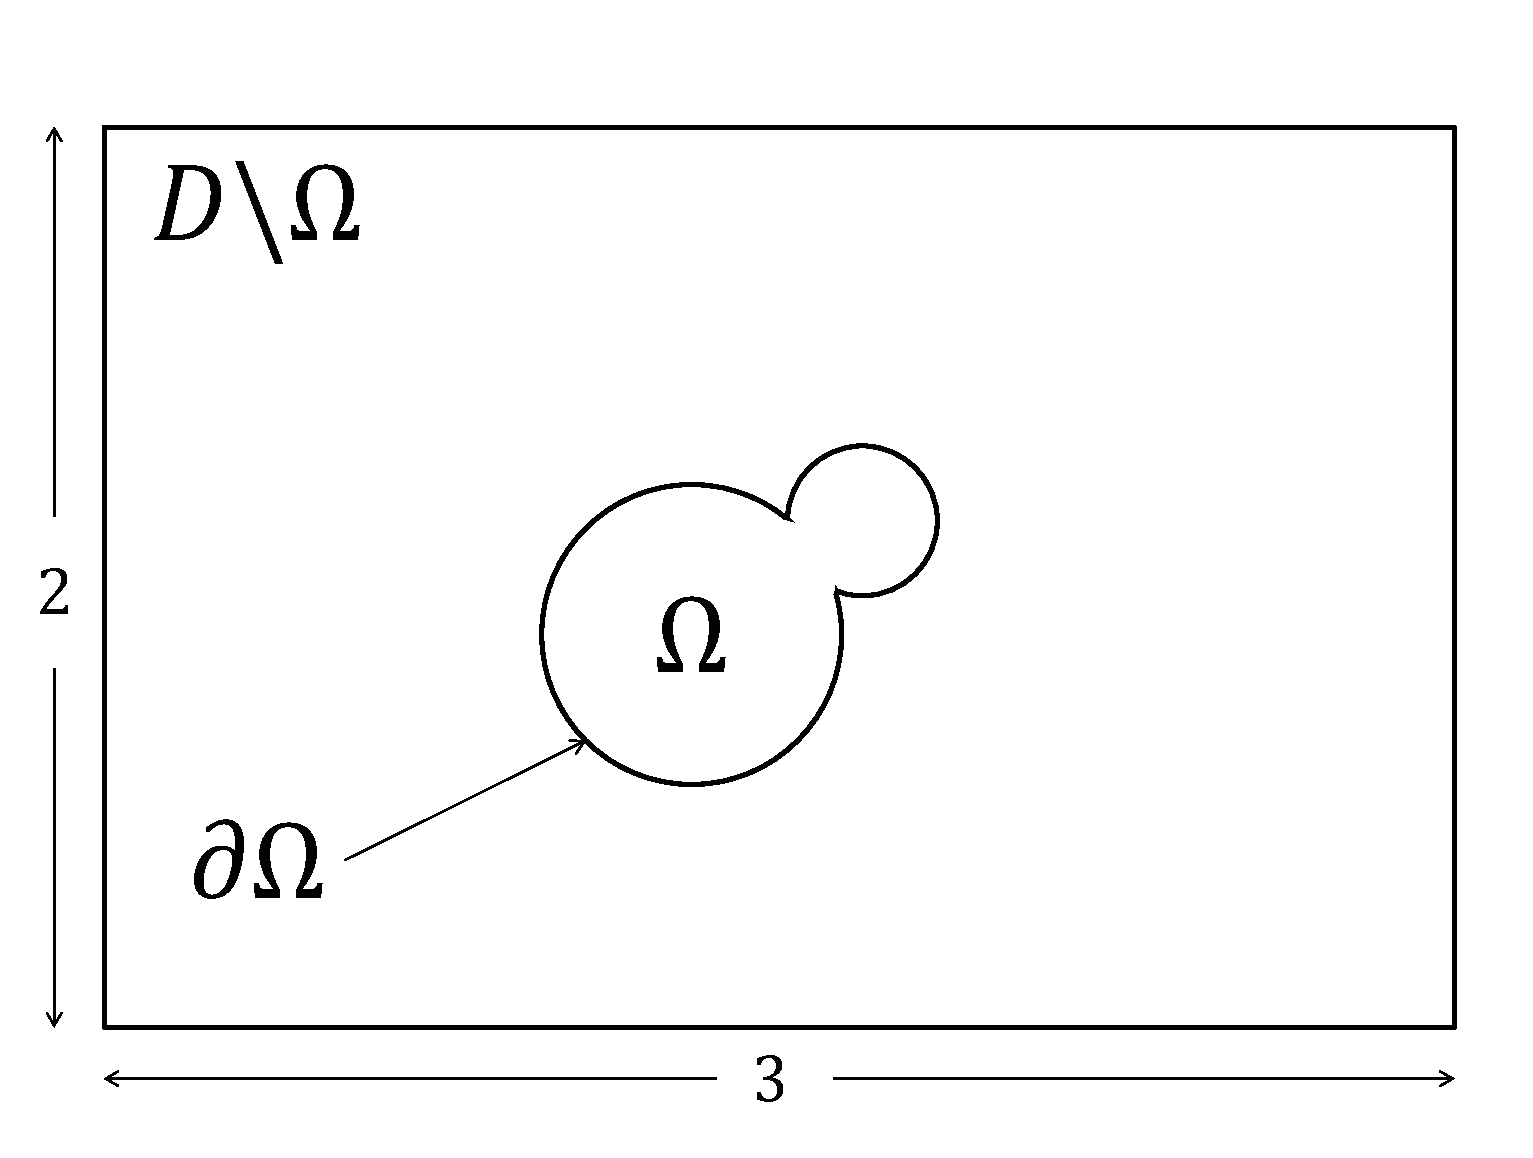
\includegraphics[width=\linewidth]{level_set_circles_3.eps}
		} &
		\subfloat[]{
			\label{fig:level_set_circle_func_075}
			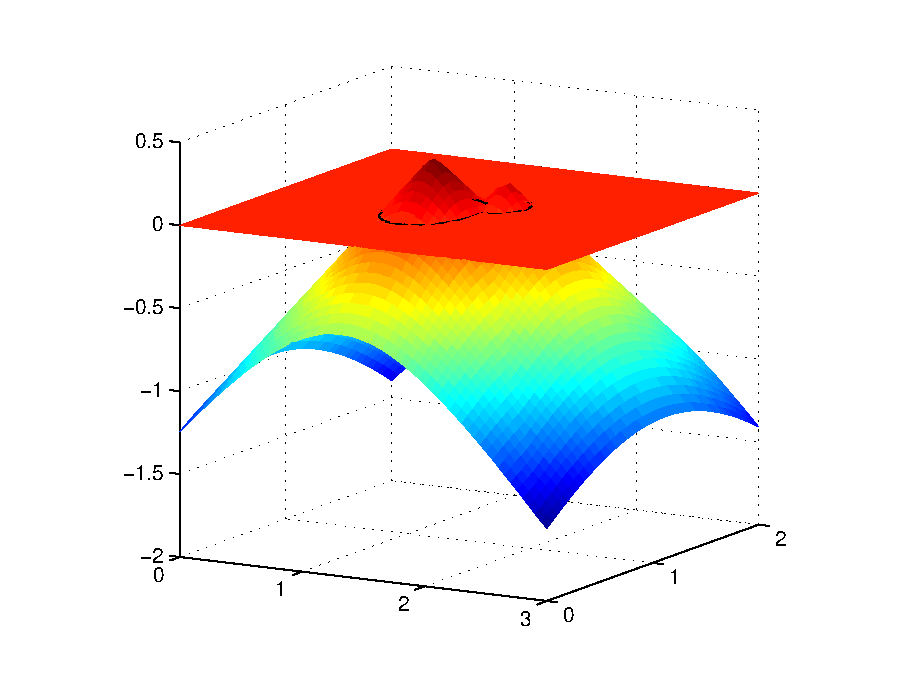
\includegraphics[width=\linewidth]{level_set_function_circles_3.eps}
		} \\
	\end{tabularx}
	\caption{Level set description of two circular inclusions with radii $0.667$ and $0.333$, respectively, moving towards each other. Level set functions can be used to describe complex topologies in a fixed mesh.}
	\label{fig:level_set_description}
\end{figure}

Multiple level set functions can be used to model more than two phase regions \ref{eq:level_set_regions}. As with the level set method itself, the use of multiple level set functions originated in image processing \citep{VC:02}. This so-called ``color'' level set method requires $m$ level set functions to model $n = 2^m$ different phase regions. For a reference on the method, the reader is referred to \citep{WW:04c,WW:05}.

The material distribution in the design domain can be determined from the phase region of the level set field. Several methods exists to describe this distribution. Density based level set methods describe the phase regions by either using element-wise constant material fractions or by mapping the level set field directly to a point \citep{YYK+:15}. These techniques are denoted as Ersatz material approaches (see Figure \ref{fig:ersatz_interpolation}) \citep{WWG:03,AJ+:05}, and while they ease the computational complexity, they lead to modeling errors. In this work, we will triangulate the element cut by the zero level set isolevel, and then perform our operations on the subdomains and on the interface (see Figure \ref{fig:XFEM_interpolation}) \citep{MM:13,VM:14}. This methodology will avoid the need to approximate material properties such as in density methods.

Regularization techniques are used in a level set optimization problem to control the geometry of the design. Among these techniques are perimeter or curvature minimization \citep{MKM+:11,YIN+:10,DLK:12}. The advantage of the level set method is that we possess a crisp definition of the phase interface, and therefore can integrate over the shape boundary $\Gamma_{\phi=0}$. These techniques will be studied in Section \ref{sec:topology_optimization_approaches_for_the_curvature_minimization_of_level_set_isocontours}.

% -----------------------------------------------------------------------------
% Topology optimization with the level set method

\subsection{Topology optimization with the level set method}

The topology of the level set field is modified by update schemes that use the sensitivities of the design variables. Several approaches exist, such as the Hamilton-Jacobi equation \citep{YNY+:10}. This work will focus on a mathematical programming approach, where the nodal values of the discrete level set field are defined as functions of the optimization design variables. Like in the filtering method of density approaches, we will define a linear filter
%
\begin{equation}
	\label{eq:smoothing_filter_XFEM}
	\phi\left(\mathbf{s}\right)=\frac{\sum_{i=1}^{N}w_{i}s_{i}}{\sum_{i=1}^{N}w_{i}}
\end{equation}

with

\begin{equation}
	\label{eq:weight_XFEM}
	w_{i}=\max \left( 0, r_{\phi} - \Vert \mathbf{x}_i - \mathbf{x} \Vert \right)
\end{equation}
%
where $\phi\left(\mathbf{s}\right)$ is the level set function at a point $\mathbf{x}$, $\mathbf{x}_{i}$ is the location of the node at which the design variable $i$ is defined, $w_{i}$ is the factor of point $\mathbf{x}$ with respect to the design variable $i$, $r_{\phi}$ is the filter radius, and $N$ is the number of nodes in the design domain. However, unlike the filter in the density approaches, this filter cannot control the minimum feature size, as discussed in Section \ref{sec:feature-size-control}.

The reader is referred to \citep{DML+:13,GP:13} for a more detailed overview of the level set method and topology optimization approaches.

% -----------------------------------------------------------------------------
% Extended finite element method

\section{Extended finite element method}
\label{sec:intro_xfem}

The extended finite element method (XFEM) is an immersed boundary technique that works on fixed meshes. The XFEM was built upon the concept of partition of unity developed by \citep{NME:NME86}, and it was originally used to model crack propagation \citep{BB:99}. Due to its ability to approximate discontinuous solutions, the method has been applied in a variety of discontinuous partial differential equations, such as multimaterial structural mechanics \citep{WW:04c,VM:14}, fluid-structure interaction \citep{GW:08}, and multi-phase flows \citep{CB:03}. The method has also been applied to shape optimization by \citep{DMJ+:06,MMF+:05,MD:07}, and to topology optimization by \citep{HMM:13,LWW:12,WWX:10,MKM+:11,MM:14,VM:14}.

The XFEM decomposes the cut elements into subdomains and interfaces that it uses to integrate the weak form of the governing equations. Figure \ref{fig:triangulation_2D} illustrates this by showing the possible decompositions of a two dimensional finite element based on its nodal level set values.
%
\begin{figure}
	\centering
	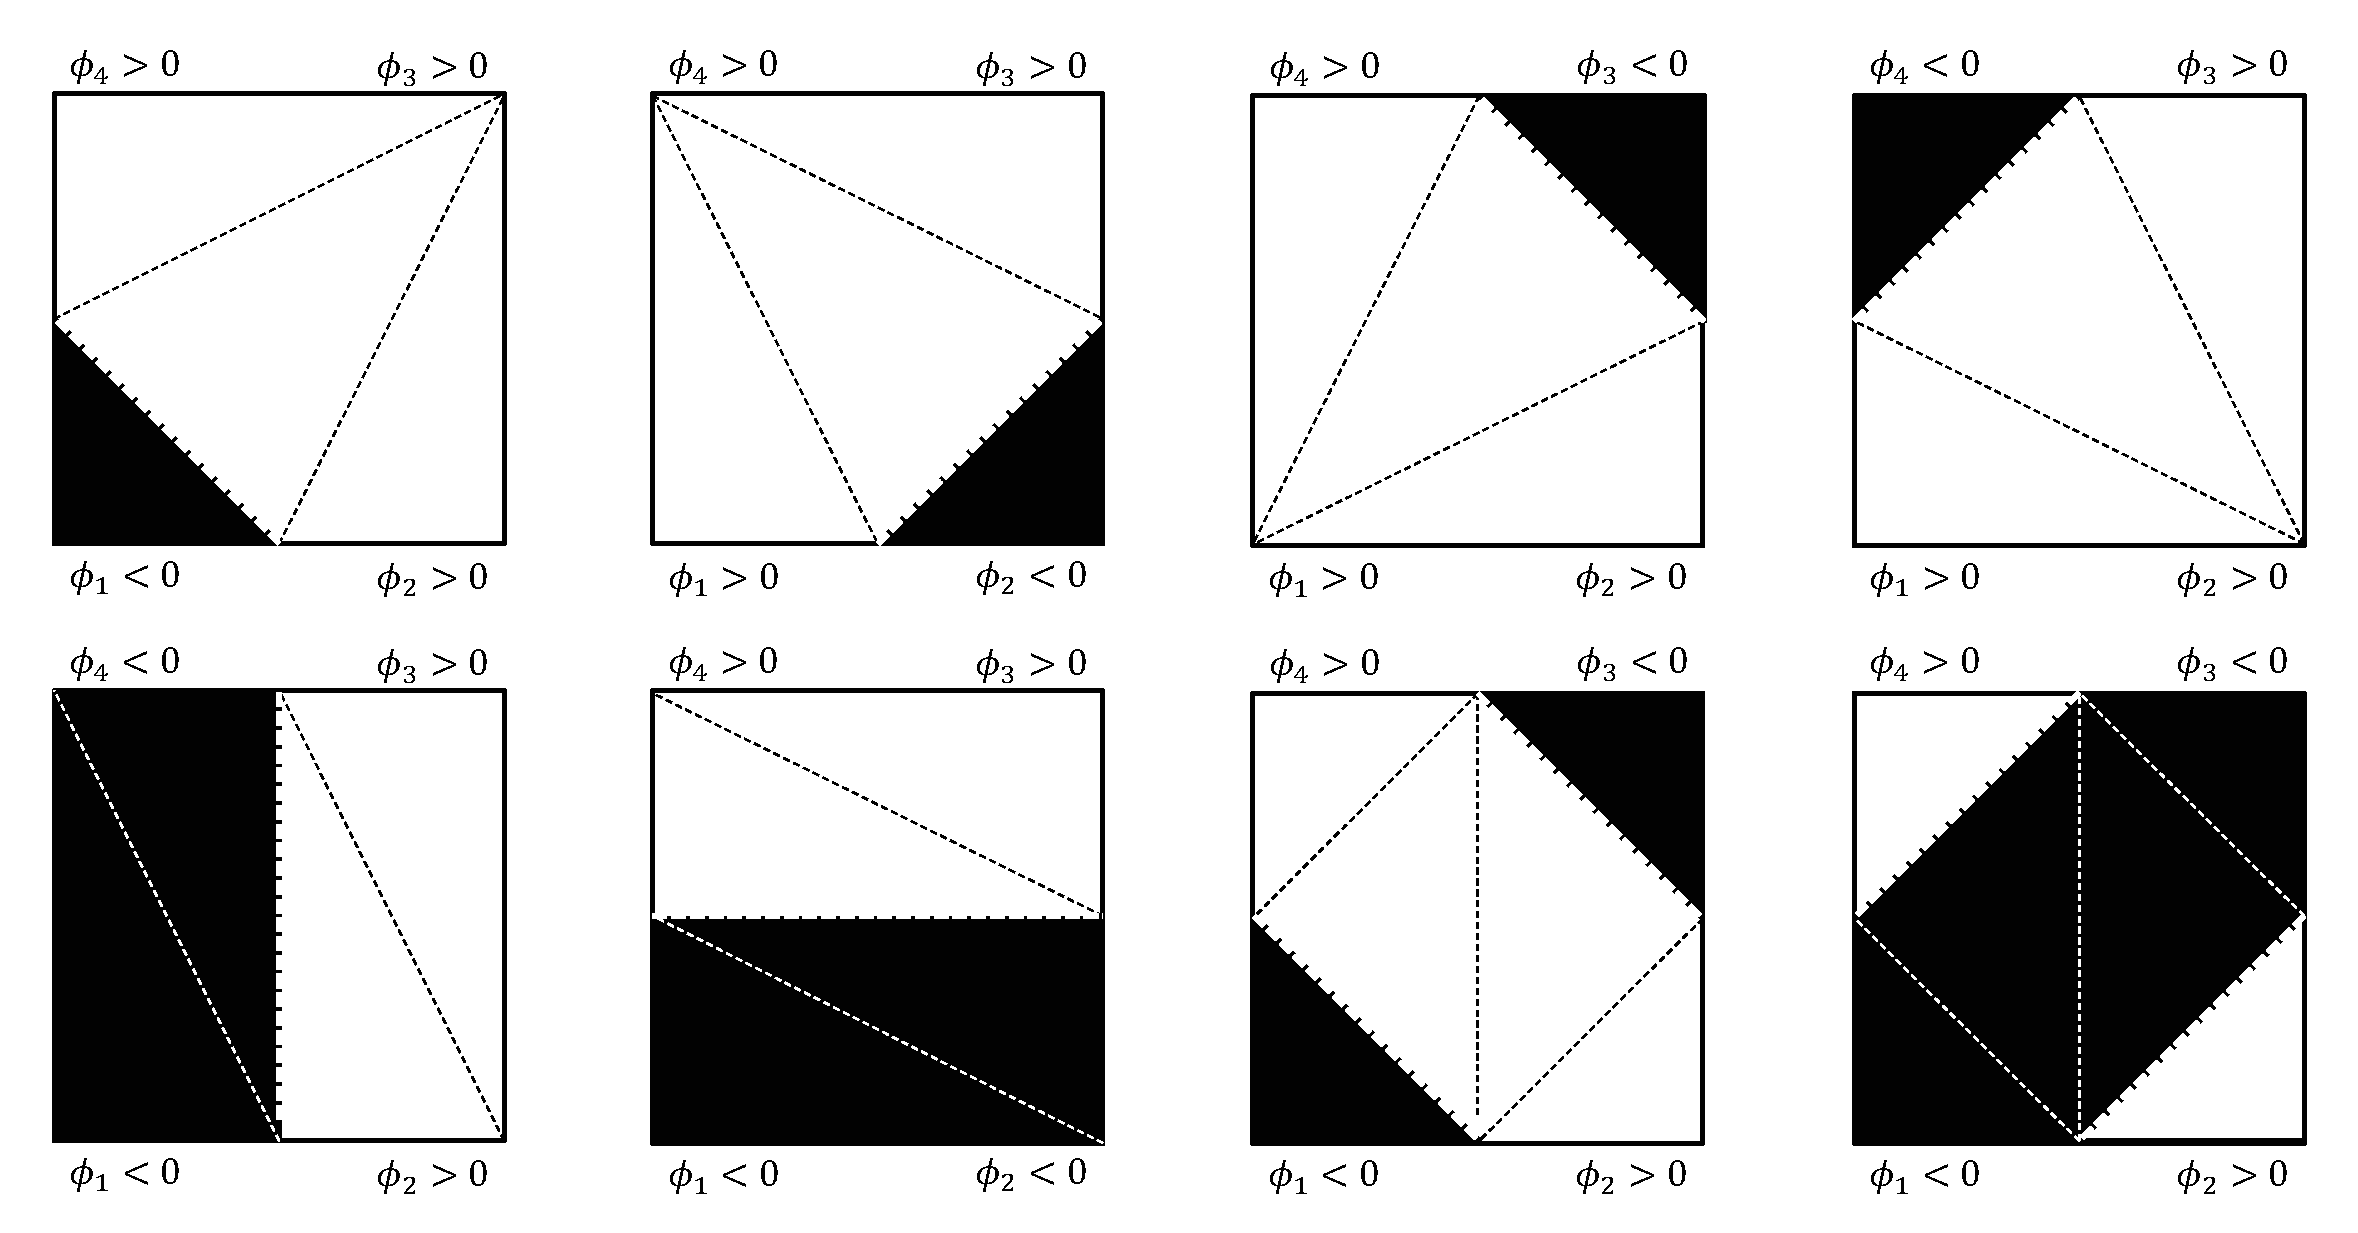
\includegraphics[width=\linewidth]{intersections_2D.eps}
	\caption{A two dimensional finite element has eight possible decompositions based on the nodal level set values.}
	\label{fig:triangulation_2D}
\end{figure}

The XFEM can model discontinuities in the solution field by augmenting the standard finite element function space with additional degrees-of-freedom, denoted ``enriched degrees-of-freedom''. To illustrate this with a quick example, consider an XFEM model that consists of a two dimensional mesh with four linear elements. The level-set distribution in Figure \ref{fig:intro_structural_model} leads to the intersection pattern shown in Figure \ref{fig:intro_physical_model}. The nodes on the left are clamped, and the right edge is subject to a constant pressure load. The node at the center of the mesh in Figure \ref{fig:intro_physical_model} will use different degrees-of-freedom to interpolate the different subdomains, and avoid artificially coupling the disconnected phase regions.
%
\begin{figure}
	\centering
	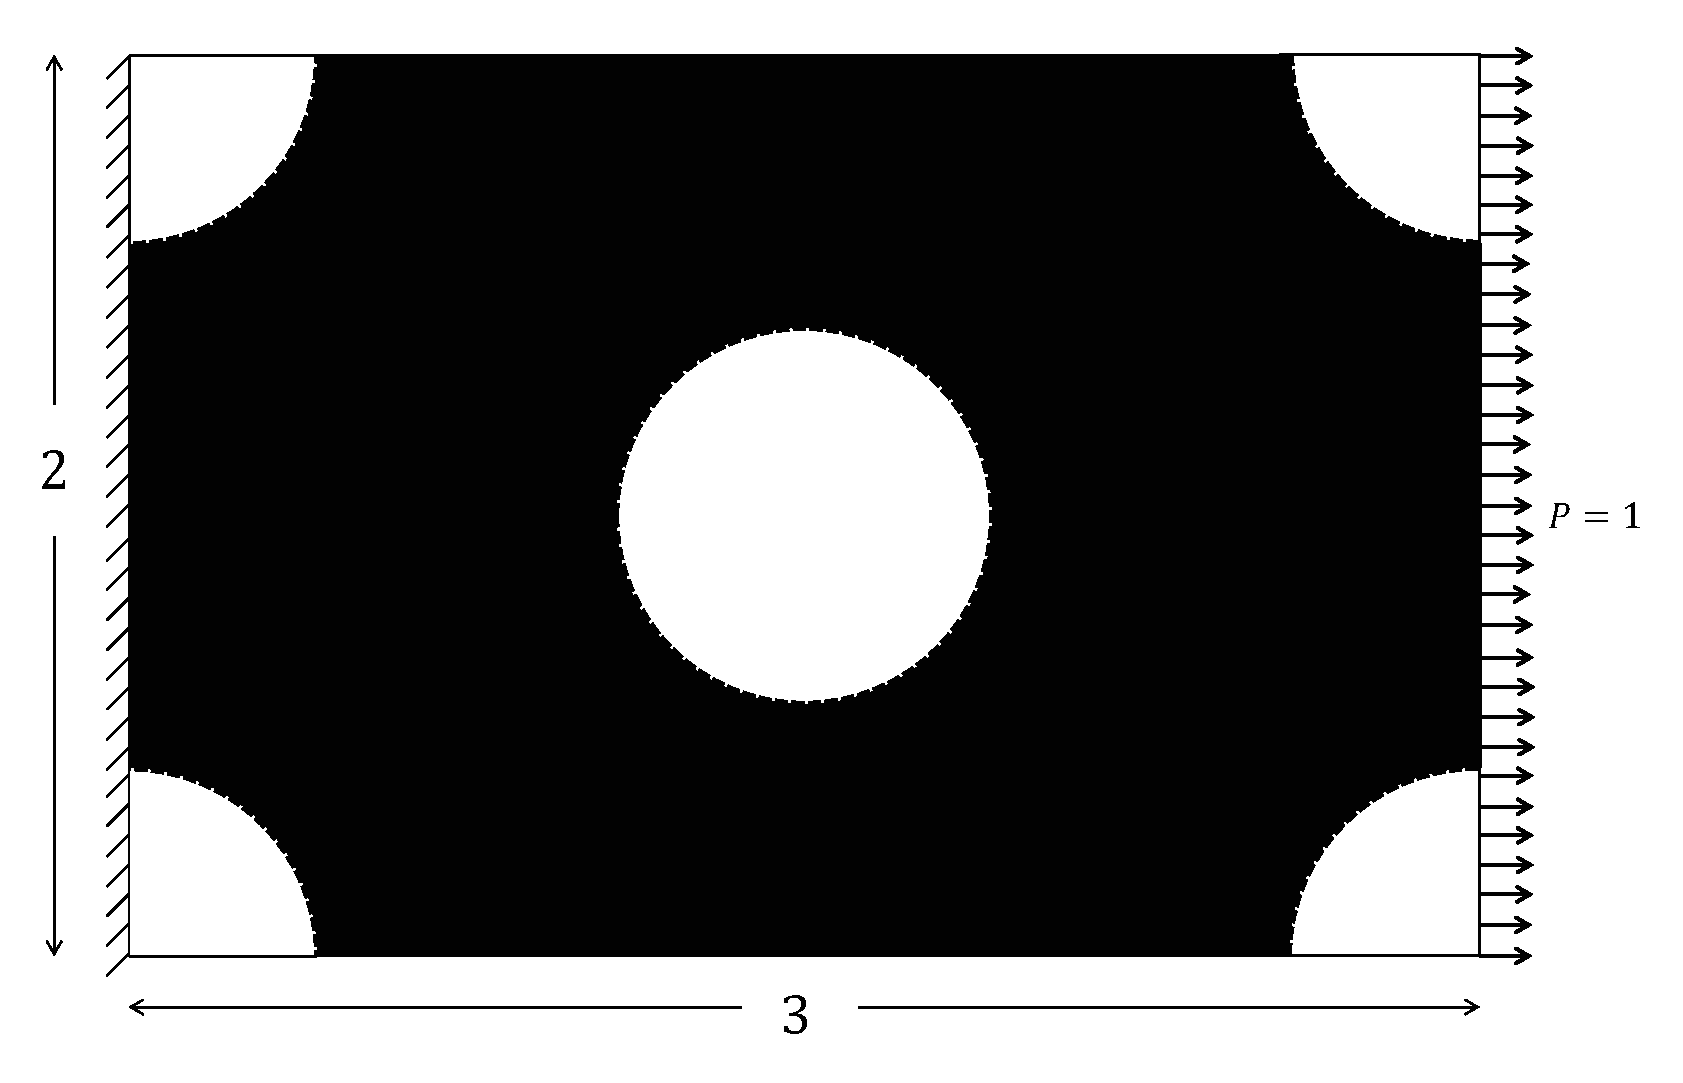
\includegraphics[width=0.75\linewidth]{structural_model.eps}
	\caption[Structural problem setup.]{Structural problem setup. The domain contains multiple level set inclusions.}
	\label{fig:intro_structural_model}
\end{figure}
%
\begin{figure}
	\centering
	\includegraphics[width=0.75\linewidth]{physical_model.eps}
	\caption[XFEM implementation example physical model]{4-element 2D mesh. Black areas: material phase 1, negative level-set value at the nodes; white areas: material phase 2, positive level-set value.}
	\label{fig:intro_physical_model}
\end{figure}

The solution space is then interpolated using the generalized enrichment formulation of \citep{HH:04}:
%
\begin{equation}
	\mathbf{u}(\mathbf{x}) = \sum \limits^{M}_{m=1} \left( H(-\phi) \sum\limits^{n}_{i=1} \mathbf{N}_i \ \mathbf{u}_{i,m}^A
														 + H( \phi) \sum\limits^{n}_{i=1} \mathbf{N}_i \ \mathbf{u}_{i,m}^B \right)
\end{equation}

where $m$ is the enrichment level, $M$ is the maximum number of enrichment levels used for each phase, $\mathbf{N}$ are the shape functions, $\mathbf{u}^l_{i,m}$ is the vector of degrees-of-freedom values at node $i$ for phase $l=[A,B]$, $\phi$ is the level set value evaluated at $\mathbf{x}$, and $H$ denotes the Heaviside function. This is illustrated in Figure \ref{fig:intro_enrichment_model} for the structural problem of Figure \ref{fig:intro_structural_model}.
%
\begin{figure}[htbp]
	\centering
	\includegraphics[width=0.9\linewidth]{enrichment_model.eps}
	\caption{The center node, denoted by the color blue, uses different degrees-of-freedom to describe the disconnected phase regions. The subscripts denote the $m$ enrichment level. The maximum number of enrichment levels used for each phase is $M=5$. A value of 0 denotes the original finite element degrees-of-freedom, while other numbers indicate additional ``enriched degrees-of-freedom''. }
	\label{fig:intro_enrichment_model}
\end{figure}

The Heaviside function $H$ depends on the level set function and is defined as follows:
%
\begin{equation}
	H(z) =
		\begin{cases}
			1 & z > 0 \\
			0 & z \le 0
		\end{cases}
\end{equation}

The Heaviside functions ``turns on/off'' the standard finite element interpolations in the particular phases. The approximation allows for discontinuities of the states $\mathbf{u}$ along the phase boundaries. Therefore, the continuity of the solution at the interface between different phase regions must be enforced. Several techniques are available in the literature, such as stabilized Lagrange multipliers (Section \ref{sec:density_and_level_set_XFEM_schemes_for_topology_optimization_of_3D_structures}) \citep{BH:10}, and the Nitsche method (Section \ref{sec:level_set_XFEM_topology_optimization_of_3D_navier_stokes_and_scalar_transport_problems}) \citep{BH:12}. More recent development include the face-oriented ghost penalty (Section \ref{sec:level_set_XFEM_topology_optimization_of_3D_navier_stokes_and_scalar_transport_problems}) by \citep{SW:14,SRG+:14,BH:12}, which aims at smoothing the gradients of the solution between cut elements. All three formulations will be studied and applied to topology optimization in this work.

For more details, refer to Sections \ref{sec:a_complete_methodology_for_the_implementation_of_XFEM_inclusive_models}, \ref{sec:discretization}, and \ref{sec:computational-considerations}. For a review of the XFEM, the user is referred to \citep{FB:10}.

% -----------------------------------------------------------------------------
% Available software

% \section{Available software}

% For the numerical modeling and simulation, we will use our in-house code, the Finite Element Multidisciplinary Optimization Code (FEMDOC). The linear algebra package is provided by Trilinos \citep{Trilinos:03}.

% -----------------------------------------------------------------------------
%
%* What is your work about?
%
%- Topology optimization approach.
%- Using the Level Set Method.
%- eXtended Finite Element Method.
%- LSM describes the geometry of the design.
%- XFEM is used to solve the PDE and measure the performance.
%- Apply methodology for complex work.
%
%* Who should care about your work?
%
%- Topology optimization community. 
%- Alternate method to homogenization methods.
%- Design engineers.
%- Surface mesh ready for three dimensional printing.
%
%* What are the goals of your thesis?
%
%- Develop robust topology optimization approach using the LSM and the XFEM methods.
%- Compare pros and cons against homogenization methods.
%- Apply methodology to real-world problem, such as ALD.
%
%* What is your overarching approach? How will you know you have accomplished your goals?
%
%- Develop methodology for triangulation, enrichment of 3D geometries (methodology section).
%- Test framework with structural problems in three dimensions (structural section).
%- Compare results with SIMP (structural section).
%- Expand to incompressible Navier-Stokes and Stokes flows, and scalar transport (fluids section).
%- Study convergence with respect to the enforcement of boundary conditions to ensure stability and coercivity.
%- Study convergence with respect to intersection configuration.
%- Study shape control and regularization techniques (curvature section).
%- Three dimensional printing (structural, fluids, curvature sections).
%- Apply methodology to ALD problem (ALD section).
%
%* Why should they care about your work?
%
%- Methodology accommodates different physics.
%- Accommodate structural, Navier-Stokes, scalar transport physics.
%- Three dimensional problems.
%- For topology optimization, it is relevant because it provides an alternate method besides homogenization methods.
%- Advantages over SIMP.
%- Explicit description of boundary for correct application of boundary conditions.
%- Regularization techniques allow shape control of the interface.
%- Prevents spurious diffusion, etc.
%- Coarser mesh leads to faster computations.
%
%* Does it enable us to solve new optimization problems or just live with coarser mesh?
%
%- Solve topology optimization problems where physics at interface is crucial.
%- ALD requires measuring temperature distribution correctly. Spurious diffusion does not help the problem.
%- Coarse mesh is good enough to describe physics at the interface.
%- In 3D, efficiency is crucial.
%
%* How is thesis proposal structured?
%
%- What sections present?
%- Mention sections are drafts of papers.
\section{Implementation}
\label{implementation}

%----------------------------------------------------------------------------------------
% Summary

\subsection{Summary}

This document outlines the procedure for building an XFEM model for a given distribution of the level-set function. The XFEM model consists of:
\begin{itemize}
\item Intersection points along elemental edges.
\item XFEM elements sub-divided into cells for integrating the weak form of the governing equations within the individual sub-domains belonging to a particular material phase.
\item Enrichment tables that define the nodal enriched degrees of freedom used to interpolate the solution within a cell.
\item Parallel implementation of building XFEM model.
\end{itemize}

%----------------------------------------------------------------------------------------
% Glossary

\subsection{Glossary}

\noindent
\textbf{computational mesh} -- standard FE mesh that defines the nodal degrees of freedom. \\
\textbf{model} -- physical entity, contains information about the XFEM elements and the level-set functions. \\
\textbf{main phase (phase)} -- phase indicating a particular material phase. \\
\textbf{sub-phase} -- the domain of a main phase can be decomposed into multiple sub-phases. \\
\textbf{intersection point} -- intersection created by the zero level-set curve cutting through an edge. \\
\textbf{point} -- geometrical entity with information about coordinates, connected cells and edges. \\
\textbf{cell} -- geometrical entity, a collection of points, owns a list of edges too. \\
\textbf{edge} -- geometrical entity with information about the points on its ends and its connected cells. \\
\textbf{Delaunay triangulation} -- triangulation of our elements using their corner nodes and intersection points. \\
\textbf{pseudo-element} -- cells created by the triangulation of the regular element. \\
\textbf{nodal cluster} -- set of elements (and their nodes) connected to a node
consistency nodes	nodes shared by multiple elements within nodal cluster. \\

%----------------------------------------------------------------------------------------
% Procedure

\subsection{Procedure overview}

The main steps are:
\begin{enumerate}
\item Build point-to-cells connectivity list (list of cells connected to a point) by looping over all cells; needs to be built only once.
\item Build edge table in mesh (list of the cell edges that stores connectivity to points and cells) by looping over all cells; needs to be built only once.
\item Build table of nodes belonging to a nodal cluster (first-order neighbors of a node; defined as all nodes belonging to elements connected to a node) by looping over all elements for a node using point-to-cell table; needs to be built only once.
\item Build edge intersection points by looping over all edges; points are stored in mesh; however, the coordinates of the intersections are copied to the XFEM element; needs to be built for each instance of a level-set distribution.
\item Delaunay triangulation of each cell based on edge intersection; needs to be built for each instance of a level-set distribution.
\item Build table of phases and sub-phases for each triangle/tetrahedron (pseudo-cells) for each triangulated element; needs to be performed for each instance of level set distribution.
\item Build enrichment table that defines which nodal degrees of freedom are used to interpolate a field within a pseudo-element.
\item Determine which degrees of freedom are used in the model.
\end{enumerate}

%\begin{figure}[htbp]
%	\centering
%	\includegraphics[scale=1]{./img/procedure_overview.png}
%	\caption[XFEM Overall Procedure]{The diagram shows the overall procedure required to implement the XFEM model.}
%	\label{fig:Overall-Procedure}
%\end{figure}

% -----------------------------------------------------------------------------
% XFEM implementation algorithms

\subsection{Implementation algorithms}
\label{sec:implementation}

Consider the following XFEM model which consists of a 4-element mesh in 2D; the nodes on the left are clamped and the right edge is subject to a constant pressure load. The level-set distribution in Figure \ref{fig:structural_model} leads to the intersection pattern shown in Figure \ref{fig:physical_model}. The mesh in Figure \ref{fig:discrete_model} shows the indices of the nodes and the cells.

\begin{figure}[htbp]
	\centering
	\includegraphics[width=0.75\linewidth]{structural_model.eps}
	\caption[Structural problem setup.]{Structural problem setup. The domain contains multiple level set inclusions.}
	\label{fig:structural_model}
\end{figure}

\begin{figure}[htbp]
	\centering
	\includegraphics[width=0.75\linewidth]{physical_model.eps}
	\caption[XFEM implementation example physical model]{4-element 2D mesh. Black areas: material phase 1, negative level-set value at the nodes; white areas: material phase 2, positive level-set value.}
	\label{fig:physical_model}
\end{figure}

\begin{figure}[htbp]
	\centering
	\includegraphics[width=0.75\linewidth]{discrete_model.eps}
	\caption[XFEM implementation example discrete model]{4-element 2D mesh. Red numbers represent the global element identifiers, blue numbers represent the global node identifiers.}
	\label{fig:discrete_model}
\end{figure}

% -----------------------------------------------------------------------------

\subsubsection{Point-to-cells connectivity table}

To build a point-to-cell table for each point in our computational mesh we loop over all base cells in the computational mesh (base cells are all cells that are not side-set cells). For each base cell we loop over all points and store the current cell index with point index. This leads to the point-to-cell connectivity table (see Table \ref{tab:point-to-cell-connectivity-table}):

\begin{table}[htbp]
	\centering
		\begin{tabular}{| l | l | l |}
		\hline
		Point Id & Number of cells connected & Cell Ids \\ \hline
		1 & 1 & 1		\\ \hline
		2 & 2 & 1,2		\\ \hline
		3 & 4 & 1,2,3,4 \\ \hline
		4 & 2 & 1,4 	\\ \hline
		5 & 1 & 2 		\\ \hline
		6 & 2 & 2,3 	\\ \hline
		7 & 1 & 3 		\\ \hline
		8 & 2 & 3,4 	\\ \hline
		9 & 1 & 4   	\\ \hline
		\end{tabular}
	\caption[Point ID to cell IDs connectivity table]{Point ID to cell IDs connectivity table}
	\label{tab:point-to-cell-connectivity-table}
\end{table}

% -----------------------------------------------------------------------------

\subsubsection{Edge table}
\label{sec:edge-computation}
To generate an edge table in our computational mesh we initially loop over all base cells. For each cell, we determine the number of edges and loop over all edges in the cell. For each edge, we check with the current element whether the edge has been created. In case the edge does not exist yet, we store the following edge information:

\begin{itemize}
\item Ids of end point of edge.
\item Ids of cells to which element is connected.
\end{itemize}

We determine the cells which are connected to an edge via the intersection of cells connected to the end points of the edge, using the point-to-cell table. The following edge table is stored with the computational mesh. 

At this point, each global edge knows the point Ids on its ends and the cell Ids of the elements it is connected to. We can use this information to create a map that links the global edge to the local edge index per element. Each element has an internal edge order list pre-built that indicates the order in which its edges are organized. For example, a QUAD4 element will have the following internal edge order list: 0 1, 1 2, 2 3, 3 0. The element also knows the point Ids that it owns (if not directly, point Ids can be obtained through the nodes). Using these two lists, we can compute which point Ids lay in each of the element's internal edges. By matching the point Ids of the global edge to the point Ids of the internal element edges, we can make a map that tells us which internal edge in an element corresponds to a global edge. This list is stored with the edge in the same manner that cell Ids are stored. Cell Ids and internal edge numbers should have a one to one correspondence.

For example, for the 4-element cluster above we would obtain 12 global edges (see Table \ref{tab:edge-table}).

\begin{table}[htbp]
	\centering
		\begin{tabular}{| l | l | l | l |}
		\hline
		Global Edge Id & Point Ids & Cell Ids & Local Edge Num \\ \hline
		1  & 1, 4 & 1   & 0 	\\ \hline
		2  & 3, 4 & 1 4 & 1, 3 	\\ \hline
		3  & 2, 3 & 1 2 & 2, 0 	\\ \hline
		4  & 1, 2 & 1   & 3 	\\ \hline
		5  & 4, 9 & 4   & 0 	\\ \hline
		6  & 8, 9 & 4   & 1 	\\ \hline
		7  & 3, 8 & 3 4 & 0, 2 	\\ \hline
		8  & 2, 5 & 2   & 3 	\\ \hline
		9  & 5, 6 & 2   & 2 	\\ \hline
		10 & 3, 6 & 2 3 & 1, 3	\\ \hline
		11 & 6, 7 & 3   & 2 	\\ \hline
		12 & 7, 8 & 3   & 1 	\\ \hline
		\end{tabular}
	\caption[Edge to points and cells IDs connectivity table]{Edge to points IDs and cells IDs connectivity table}
	\label{tab:edge-table}
\end{table}

The table shows, for example, that the global edge 2 is defined by the point Ids 3 and 4 and is connected to cells with Ids 1 and 4. For cell id 1, it is the local edge 1 (counting from zero CCW starting at the bottom) and for cell id 4 it is local edge 3 (Figure \ref{fig:edge-discretization}).

\begin{figure}[htbp]
	\centering
	\includegraphics[width=0.7\linewidth]{edge_discretization.eps}
	\caption[Edge discretization of XFEM model example]{Edge representation in a QUAD4 element. Green edges represent the local edge index at the element.}
	\label{fig:edge-discretization}
\end{figure}

% -----------------------------------------------------------------------------

\subsubsection{Nodal clusters}

To determine the enrichment level used to interpolate fields within the XFEM elements we need to determine the first-order nodal neighbors of a node. This is the set of nodes that belong to the elements connected to a node. In addition, we need to identify the nodes that belong to two or more elements; we refer to these nodes as consistency nodes. Consistency nodes are simply the nodes in a nodal cluster (nodes of the connected elements of a main node) that are shared by more than one element in the nodal cluster. This information can be obtained by looping over the connected elements of a node, and obtaining the node list for each element. 

% -----------------------------------------------------------------------------

\subsubsection{Determine intersection points}

The intersection points are defined by the zero level-set values. We loop over all edges defined in the edge table created in Step 2 and compute the intersection points along the edge using the nodal level-set information of the edge endpoints.  The coordinates of the intersection points are then sent to all elements connected to the edge and stored in the corresponding XFEM element. (see Figure \ref{fig:intersection_point}). NOTE: Since edges only know of the cells connected to it, we use a cell-to-element map in order to be able to send this information to the XFEM elements. This is owned by the model.

\begin{figure}[htbp]
	\centering
	\includegraphics[width=\linewidth]{intersection_point.eps}
	\caption[Intersection point computation]{Mapping of the intersection points to the elements. An edge contains two nodes that have level set values of opposite sign. The location of the intersection point is labeled with an ``X'' in the figure. The information of the intersection point is sent to all the neighboring elements of the edge.}
	\label{fig:intersection_point}
\end{figure}

% -----------------------------------------------------------------------------

\subsubsection{Delaunay triangulation and assignment of main and sub-phases to pseudo-elements}

We loop over all elements in the model and, if intersected, we perform a Delaunay triangulation, using the corner nodes and the edge intersection points stored with the elements in Step 3. The Delaunay triangulation requires only the coordinates of the element corner and edge intersection points. The Delaunay triangulation will return a list of triangles for 2D or tetrahedrons for 3D problems. 

% -----------------------------------------------------------------------------

\subsubsection{Main phase and sub-phase}
\label{sec:main-phase-sub-phase}

We assign a main and sub-phase to each triangle/tetrahedron. The main phase is determined based on the average main-phase value of the pseudo-element.  In case the average is zero, we apply an exception rule (TBD). The sub-phase information is based on the connectivity of pseudo-elements which belong to the same main phase and is computed via a \href{http://en.wikipedia.org/wiki/Flood_fill}{flood-fill algorithm}. To this end we collect the pseudo-elements into a pseudo-mesh; each triangulated XFEM element has its own pseudo-mesh which consists of the points and the connectivity of the pseudo-elements.
The main steps (Figure \ref{fig:subphase_algorithm}) of the flood-fill algorithm used are:

\begin{itemize}
\item Build edge table for pseudo-elements of current XFEM element, analogue to Step \ref{sec:edge-computation}.
\item Loop over all elements that have not been assigned a sub-phase:
	\begin{itemize}
	\item Find unprocessed element; recursively find neighbors with same main-phase; assign lowest unassigned sub-phase to elements found in search process.
	\end{itemize}
\end{itemize}

\begin{figure}[H]
	\centering
	\begin{tabularx}{\linewidth}{XXX}
		\subfloat[Start with the first subphase value of the first main phase. Do so by selecting the first cell in the triangulation list without a value assigned.]{
			\label{fig:subphase_algorithm_1}
			\includegraphics[width=\linewidth]{subphase_algorithm_1.eps}
		} &
		\subfloat[Look for connected cells through edges. If two cells share the same main phase and are connected, then they have the same subphase.]{
			\label{fig:subphase_algorithm_2}
			\includegraphics[width=\linewidth]{subphase_algorithm_2.eps}
		} &
		\subfloat[Move on to the next cell in the list that shares the same main phase value, and continue checking the connectivity.]{
			\label{fig:subphase_algorithm_3}
			\includegraphics[width=\linewidth]{subphase_algorithm_3.eps}
		} \\
		\subfloat[Once the connectivity for the specific subphase of the main phase is achieved, check if additional cells have the same main phase but different subphase. If there are not any cells with the same main phase, move on the next main phase.]{
			\label{fig:subphase_algorithm_4}
			\includegraphics[width=\linewidth]{subphase_algorithm_4.eps}
		} &
		\subfloat[Select the first subphase of the second main phase. Repeat steps 1 through 3.]{
			\label{fig:subphase_algorithm_5}
			\includegraphics[width=\linewidth]{subphase_algorithm_5.eps}
		} &
		\subfloat[Once the connectivity for a subphase is computed, increase the subphase value within the main phase. Look for cells in the triangulation list that have not been processed yet, and check their connectivity.]{
			\label{fig:subphase_algorithm_6}
			\includegraphics[width=\linewidth]{subphase_algorithm_6.eps}
		}
	\end{tabularx}
	\caption[Subphase computation algorithm.]{Subphase computation algorithm. Refer to section \ref{sec:main-phase-sub-phase} for a more detailed description.}
	\label{fig:subphase_algorithm}
\end{figure}

For Figure \ref{fig:subphase_algorithm}, we would get the list in table \ref{tab:main-phase-sub-phase-table}:

\begin{table}[htbp]
	\centering
		\begin{tabular}{| l | l | l |}
		\hline
		Triangle number & Main Phase & Sub-Phase \\ \hline
		1 & 1 & 0 \\ \hline
		2 & 1 & 0 \\ \hline
		3 & 1 & 0 \\ \hline
		4 & 1 & 0 \\ \hline
		5 & 2 & 1 \\ \hline
		6 & 2 & 2 \\ \hline
		\end{tabular}
	\caption[Main-phase and sub-phase table for pseudo-elements]{Main-phase and sub-phase table for pseudo-elements.}
	\label{tab:main-phase-sub-phase-table}
\end{table}

We have 6 different triangles generated by Delaunay triangulation. By convention, the order of the triangles is determined after the triangulation so that all phase 1 ones are located at the top, followed by the phase 2 triangles. Each triangle is assigned a main phase and sub-phase (see Table \ref{tab:main-phase-sub-phase-table}); the assignment is stored, using a one-to-one map by the XFEM element.

% -----------------------------------------------------------------------------

\subsubsection{Nodal enrichments for pseudo-elements}

To interpolate fields in the XFEM elements we need to determine which nodal enrichments are used within each pseudo element.  The enrichments need to be chosen such that the interpolations are continuous across adjacent elements within the same main phase and unique within pseudo elements of the main sub-phase but topologically disconnected.

The main concept of the procedure is to clearly separate element-level and node-level operations. This separation enables the parallelization of the procedure. The first step is to determine the enrichment levels a particular node will use to interpolate fields in the triangulated elements with a particular sub-phase. This step is done by looping over all nodes. The result of this loop is a map that links the sub-phase information of an element to an enrichment level for each node of the element. In a second step we loop over all elements to update the enrichment levels of pseudo-element based on the map built previously.

Looping over all nodal clusters, we build the following node-element table. The entries in the table are the sub-phases at the nodes within each element. The consistency node numbers are marked by a ``C''. Consistency nodes can be identified by nodes which have entries in more than one column; so they can be identified easily on the fly.

Two conditions, consistency and uniqueness, must be satisfied to ensure the assigned sub-phases are consistent across the nodal cluster. The consistency condition is satisfied if all sub-phases in a row are the same. The uniqueness condition is satisfied if the sub-phase of each set of connected nodes is unique in the cluster.

\begin{table}[htbp]
	\centering
		\begin{tabular}{| l | p{2cm} | p{2cm} | p{2cm} | p{2cm} |}
		\hline
		Nodes/Elements & 1 & 2 & 3 & 4 \\ \hline
		1 		& 14	&		&		&		 \\ \hline
		2 ``C''	&  0	&  0	&		&		 \\ \hline
		3 ``C''	& 15	& 14	& 14	& 15	 \\ \hline
		4 ``C''	&  0	&		&		&  0 	 \\ \hline
		5		& 		& 15	&		& 		 \\ \hline
		6 ``C''	&  		&  0	&  0	&		 \\ \hline
		7		&		& 		& 15	&		 \\ \hline
		8 ``C''	&		&  		&  0	&  0	 \\ \hline
		9		&		&		&		& 14	 \\ \hline
		\end{tabular}
	\caption[Initial node-element table]{Initial node-element table.}
	\label{tab:initial-node-element-table}
\end{table}

The initial node-element table (see Table \ref{tab:initial-node-element-table}) shows that the consistency condition is not satisfied since node 3 is inconsistent. Also, nodes 5 and 7, for example, should be assigned a unique sub-phase. Therefore the uniqueness condition is also not satisfied. To ensure both conditions we build a second table and where we iteratively correct the sub-phase until all conditions are satisfied. Note that the consistency and uniqueness checks are not needed for a 1 element cluster. The correction procedure is as follows:

\begin{enumerate}
\item Initialize a list of all sub-phase possible; mark them as unused; initialize a list of checked nodes. Mark all nodes as unchecked; build list of consistency nodes.
\item Ensure consistency: Repeat the following steps until all consistency nodes are checked.
	\begin{itemize}
	\item Select node: Start with the center node, which must be a consistency node (remember that this consistency and uniqueness check will not be applied for a one-element cluster). Otherwise select the first unchecked consistency node.
	\item Select sub-phase: Select the lowest unused sub-phase. Mark the selected sub-phase as used (keep consistency of sub-phase to the respective main phase).
	\item Identify connected consistency nodes and connected unique nodes:
		\begin{itemize}
		\item For each element to which the selected node belongs, connected nodes have the same sub-phase as the selected node has for this particular element. Select the connected nodes which may be either consistency or unique nodes. 
		\item In order to identify all connected consistency and unique nodes, search the connected elements for additional connected consistency and unique nodes.
		\item The above process requires recursively (a) searching for nodes within an element with the same sub-phase and (b) identifying elements that share consistency nodes. Note: the sub-phase id might change between elements if the sub-phases are not consistent yet for a consistency node.
		\end{itemize}
	\item Assign sub-phase: Assign the selected sub-phase to all connected nodes identified in the search process described above. For any value that needs to be changed, flip sub-phases for that element. Mark connected nodes as checked.
	\end{itemize}

\begin{table}[htbp]
	\centering
		\begin{tabular}{| l | p{2cm} | p{2cm} | p{2cm} | p{2cm} |}
		\hline
		Nodes/Elements & 1 & 2 & 3 & 4 \\ \hline
		1 		& 14 $\to$ 15	&		&		&		 		\\ \hline
		2 ``C''	&  0			&  0	&		&		 		\\ \hline
		3 ``C''	& 15 $\to$ 14	& 14	& 14	& 15$\to$ 14 	\\ \hline
		4 ``C''	&  0			&		&		&  0 	 		\\ \hline
		5		& 				& 15	&		& 		 		\\ \hline
		6 ``C''	&  				&  0	&  0	&		 		\\ \hline
		7		&				& 		& 15	&		 		\\ \hline
		8 ``C''	&				&  		&  0	&  0	 		\\ \hline
		9		&				&		&		& 14$\to$ 15	\\ \hline
		\end{tabular}
	\caption[Flipping the enrichment levels]{Flipping the enrichment levels to keep consistency.}
	\label{tab:flipping-enrichment-levels-table}
\end{table}

\item Ensure uniqueness: Loop through the remaining unchecked nodes. For each element, collect the unique nodes with an unused sub-phase, assign the next unused sub-phase to these nodes and check the sub-phase as being used. Here nodes 1, 5, 7, and 9 are assigned the sub-phase 16, 17, and 18, respectively (node 1 was flipped initially, but it was not marked as checked). The outcome of the above correction procedure is Table \ref{tab:final-node-element-table}:

\begin{table}[htbp]
	\centering
		\begin{tabular}{| l | p{2cm} | p{2cm} | p{2cm} | p{2cm} |}
		\hline
		Nodes/Elements & 1 & 2 & 3 & 4 \\ \hline
		1 		& 15		&		&		&		 \\ \hline
		2 ``C''	&  0		&  0	&		&		 \\ \hline
		3 ``C''	& 14		& 14	& 14	& 14	 \\ \hline
		4 ``C''	&  0		&		&		&  0 	 \\ \hline
		5		& 			& 16	&		& 		 \\ \hline
		6 ``C''	&  			&  0	&  0	&		 \\ \hline
		7		&			& 		& 17	&		 \\ \hline
		8 ``C''	&			&  		&  0	&  0	 \\ \hline
		9		&			&		&		& 18	 \\ \hline
		\end{tabular}
	\caption[Final node-element table]{The result of the enrichment algorithm. Nodes that are shared across elements receive the same enrichment level.}
	\label{tab:final-node-element-table}
\end{table}

\item Using the original and the corrected node-element tables we can build the map for the central point (here node ID 3). See Table \ref{tab:element-to-enrichment-table}. The rows correspond to the elements, the columns list the original sub-phases, and the entries are the enrichment levels used by the central node. When building this table we check that the map is consistent within itself (the same sub-phases within each are assigned to the same enrichments).

\begin{table}[htbp]
	\centering
		\begin{tabular}{| l | p{2cm} | p{2cm} | p{2cm} | p{2cm} |}
		\hline
		For Node 3:		& 0	& 14	& 15\\
		Element / Enrichment level & & &\\ \hline
		1 & 0 & 15 & 14 \\ \hline
		2 & 0 & 14 & 16 \\ \hline
		3 & 0 & 14 & 17 \\ \hline
		4 & 0 & 18 & 14 \\ \hline
		\end{tabular}
	\caption[Element to enrichment table]{Element to enrichment table for node ID 3. This table shows the initial enrichments node 3 received during the sub-phase algorithm and the enrichment levels after the enrichment algorithm.}
	\label{tab:element-to-enrichment-table}
\end{table}

\item With this map we can loop over all elements and assign enrichment levels for each node to each pseudo-element, based on their sub-phase information.
\end{enumerate}

% -----------------------------------------------------------------------------

\subsubsection{Determine degrees-of-freedom used}

The last step in the algorithm is to flag which enrichment levels each node will use for interpolation. For example, in our test case, node 3 will have enrichment levels 0, 14, 15, 16, 17, 18 active.

% -----------------------------------------------------------------------------

\subsubsection{Implementation example 2}

\begin{figure}[H]
	\centering
	\begin{tabularx}{0.75\linewidth}{X}
		\subfloat[Discrete model.]{
			\label{fig:physical_model_2}
			\includegraphics[width=\linewidth]{physical_model_2.eps}
		} \\
		\subfloat[Mesh information.]{
			\label{fig:discrete_model_2}
			\includegraphics[width=\linewidth]{discrete_model.eps}
		}
	\end{tabularx}
	\caption[XFEM implementation example 2.]{XFEM implementation configuration 2.}
	\label{fig:implementation_example_2}
\end{figure}

\begin{table}[H]
	\centering
		\begin{tabular}{| l | p{2cm} | p{2cm} | p{2cm} | p{2cm} |}
		\hline
		Nodes/Elements & 1 & 2 & 3 & 4 \\ \hline
		1 		&  0		&		&		&		 \\ \hline
		2 ``C''	& 14		& 14	&		&		 \\ \hline
		3 ``C''	&  0		&  0	&  0	&  0	 \\ \hline
		4 ``C''	&  0		&		&		&  0 	 \\ \hline
		5		& 			& 14	&		& 		 \\ \hline
		6 ``C''	&  			& 14	& 14	&		 \\ \hline
		7		&			& 		& 14	&		 \\ \hline
		8 ``C''	&			&  		& 14	& 14	 \\ \hline
		9		&			&		&		&  0	 \\ \hline
		\end{tabular}
	\caption[Initial node-element table configuration 2]{Initial node-element table for configuration 2.}
	\label{tab:initial-node-element-table-configuration-2}
\end{table}

\begin{table}[H]
	\centering
		\begin{tabular}{| l | p{2cm} | p{2cm} | p{2cm} | p{2cm} |}
		\hline
		Nodes/Elements & 1 & 2 & 3 & 4 \\ \hline
		1 		&  0		&		&		&		 \\ \hline
		2 ``C''	& 14		& 14	&		&		 \\ \hline
		3 ``C''	&  0		&  0	&  0	&  0	 \\ \hline
		4 ``C''	&  0		&		&		&  0 	 \\ \hline
		5		& 			& 14	&		& 		 \\ \hline
		6 ``C''	&  			& 14	& 14	&		 \\ \hline
		7		&			& 		& 14	&		 \\ \hline
		8 ``C''	&			&  		& 14	& 14	 \\ \hline
		9		&			&		&		&  0	 \\ \hline
		\end{tabular}
	\caption[Final node-element table configuration 2]{Final node-element table for configuration 2.}
	\label{tab:final-node-element-table-configuration-2}
\end{table}

\begin{table}[H]
	\centering
		\begin{tabular}{| l | p{2cm} | p{2cm} | p{2cm} |}
		\hline
		For Node 3:		& 0	& 14 \\
		Element / Enrichment level & & \\ \hline
		1 & 0 & 14 \\ \hline
		2 & 0 & 14 \\ \hline
		3 & 0 & 14 \\ \hline
		4 & 0 & 14 \\ \hline
		\end{tabular}
	\caption[Element to enrichment table configuration 2]{Enrichment level map for configuration 2.}
	\label{tab:element-to-enrichment-table-2}
\end{table}

% -----------------------------------------------------------------------------

\subsubsection{Implementation example 3}

\begin{figure}[H]
	\centering
	\begin{tabularx}{0.75\linewidth}{X}
		\subfloat[Discrete model.]{
			\label{fig:physical_model_3}
			\includegraphics[width=\linewidth]{physical_model_3.eps}
		} \\
		\subfloat[Mesh information.]{
			\label{fig:discrete_model_3}
			\includegraphics[width=\linewidth]{discrete_model.eps}
		}
	\end{tabularx}
	\caption[XFEM implementation example 3.]{XFEM implementation configuration 3.}
	\label{fig:implementation_example_3}
\end{figure}

\begin{table}[H]
	\centering
		\begin{tabular}{| l | p{2cm} | p{2cm} | p{2cm} | p{2cm} |}
		\hline
		Nodes/Elements & 1 & 2 & 3 & 4 \\ \hline
		1 		&  0		&		&		&		 \\ \hline
		2 ``C''	& 15		& 14	&		&		 \\ \hline
		3 ``C''	&  0		&  0	&  0	&  0	 \\ \hline
		4 ``C''	& 14		&		&		&  0 	 \\ \hline
		5		& 			& 14	&		& 		 \\ \hline
		6 ``C''	&  			& 14	& 14	&		 \\ \hline
		7		&			& 		& 14	&		 \\ \hline
		8 ``C''	&			&  		& 14	& 15	 \\ \hline
		9		&			&		&		&  0	 \\ \hline
		\end{tabular}
	\caption[Initial node-element table configuration 3]{Initial node-element table for configuration 3.}
	\label{tab:initial-node-element-table-configuration-3}
\end{table}

\begin{table}[H]
	\centering
		\begin{tabular}{| l | p{2cm} | p{2cm} | p{2cm} | p{2cm} |}
		\hline
		Nodes/Elements & 1 & 2 & 3 & 4 \\ \hline
		1 		&  0		&		&		&		 \\ \hline
		2 ``C''	& 14		& 14	&		&		 \\ \hline
		3 ``C''	&  0		&  0	&  0	&  0	 \\ \hline
		4 ``C''	& 15		&		&		& 15	 \\ \hline
		5		& 			& 14	&		& 		 \\ \hline
		6 ``C''	&  			& 14	& 14	&		 \\ \hline
		7		&			& 		& 14	&		 \\ \hline
		8 ``C''	&			&  		& 14	& 14	 \\ \hline
		9		&			&		&		&  0	 \\ \hline
		\end{tabular}
	\caption[Final node-element table for configuration 3]{Final node-element table for configuration 3.}
	\label{tab:final-node-element-table-configuration-3}
\end{table}

\begin{table}[H]
	\centering
		\begin{tabular}{| l | p{2cm} | p{2cm} | p{2cm} |}
		\hline
		For Node 3:		& 0	& 14 & 15\\
		Element / Enrichment level & & & \\ \hline
		1 & 0 & 15 & 14	\\ \hline
		2 & 0 & 14 &   	\\ \hline
		3 & 0 & 14 &   	\\ \hline
		4 & 0 & 15 & 14	\\ \hline
		\end{tabular}
	\caption[Element to enrichment table configuration 3]{Enrichment level map for configuration 3.}
	\label{tab:element-to-enrichment-table-3}
\end{table}

% -----------------------------------------------------------------------------

\subsection{Solving the problem}

In the previous section, our algorithms determined which additional enriched degrees-of-freedom each node requires to account for the discontinuities in the elements. We will study our enrichment strategy with a heat conduction problem. To capture the discontinuities along the phase boundaries, we enrich the standard finite element approximation with additional shape functions. We adopt the generalized enrichment strategy of \citet{MM:13} which resolves consistently the temperature fields in the presence of small features and does not suffer from artificially coupling disconnected phases.
%
\begin{equation}
	u(\mathbf{x}) = \sum \limits^{M}_{m=1} \left( H(-\phi) \sum\limits^{n}_{i=1} \mathbf{N}_i \ u_{i,m}^A
														 + H( \phi) \sum\limits^{n}_{i=1} \mathbf{N}_i \ u_{i,m}^B \right)
\end{equation}

where $m$ is the enrichment level, $M$ is the maximum number of enrichment levels used for each phase, $\mathbf{N}$ are the shape functions, $u^l_{i,m}$ is the vector of nodal temperature values at node $i$ for phase $l=[A,B]$, $\phi$ is the level set value evaluated at the integration point, and $H$ denotes the Heaviside function.

The Heaviside function $H$ depends on the level set function and is defined as follows:
%
\begin{equation}
	H(z) =
		\begin{cases}
			1 & z > 0 \\
			0 & z \le 0
		\end{cases}
\end{equation}

The Heaviside functions ``turns on/off'' the standard finite element interpolations in the particular phases. The approximation allows for discontinuities of the temperatures along the phase boundaries. Therefore the continuity is enforced weakly via the stabilized Lagrange multiplier method.

% -----------------------------------------------------------------------------

\subsection{Preconditioner}

When a sub-domain of a material phase is too small (around $O(\epsilon^{1/2})$), the Jacobian matrix will be ill-conditioned. To solve this shortcoming, it is necessary to scale the matrix with another preconditioning matrix. This scaling matrix will be a function of the level-set field.

The preconditioner $\pmb{T}$ will have a scaling value for each degree of freedom in the problem. To obtain these values, we check which enriched degrees of freedom each node uses. Then, we proceed to compute the integral of the shape function for the node with respect to the material sub-domain that requires said enriched degree-of-freedom. Because a node will have different scaling values across multiple elements, there are four preconditioner implementations available to compute the scaling value in a nodal cluster:

\begin{itemize}
\item Maximum value of integrals of shape functions
\item Sum of values of integrals of shape functions
\item Maximum value of integrals of the derivatives of the shape functions
\item Sum of values of integrals of the derivatives of the shape functions
\end{itemize}

The third preconditioner approach will be used in this study. The matrix $\pmb{T}$ is a diagonal matrix built by integrating the spatial derivatives of the shape functions over the nodal support of nodes connected to an intersected element. The diagonal components of the matrix are defined as:
%
\begin{equation}
	\pmb{T}_{i,m}^{l} = \left( \max_{e \in E_{i}} \frac { \int_{\mathcal{D}_l^e} \nabla \mathbf{N}_i(\mathbf{x}) \cdot
	\nabla
	\mathbf{N}_i(\mathbf{x}) \,d\mathbf{x}}{\int_{\mathcal{D}^e} \nabla \mathbf{N}_i(\mathbf{x}) \cdot \nabla
	\mathbf{N}_i(\mathbf{x}) \,d\mathbf{x}} \right)^{-1/2}
\end{equation}
%
where $\pmb{T}_{i,m}^{l}$ corresponds to the degree-of-freedom $\mathbf{u}_{i,m}^{l}$, $i$ is the node index, $l=[A,B]$ is the material phase, $m$ is the enrichment level, $E_{i}$ is the set of elements connected to node $i$, and $\mathcal{D}_l^e$ is the element domain of phase $l$. The components of the matrix increase as the region of influence of a degree-of-freedom decreases. The entries $\pmb{T}_{i,m}^{l}$ of nodes $i$ that are not connected to at least one intersected element are set to one.

To avoid numerical issues due to large values for the components of $\pmb{T}$, the degrees of freedom associated with the diagonal entry $\pmb{T}_{i,m}^{l}$ are constrained to zero if the following condition is satisfied:
%
\begin{equation}
	\pmb{T}_{i,m}^{l} \ge T_{tol}
\end{equation}
%
where $T_{tol}$ is $10^9$ for this study.

At this point, there is one scaling value for each degree-of-freedom in the system. These scaling values are applied to the solution vector before the computation of the residual. After the residual is computed, they are both unscaled and then the new solution vector is computed. 
\section{Corroboration and results}
\label{corroboration_results}

% -----------------------------------------------------------------------------
% Methodology

\subsection{Methodology}

Two formulations were used to corroborate the results of the XFEM implementation.

Equation \ref{eq:interface-error} computes the difference in solutions at the discontinuity. Since the model we have implemented is based on inclusions and not crack propagation, this interface error should approach zero as the mesh gets finer.
%
\begin{equation}
	\sqrt{\frac{\sum_{\mathrm{element}} \sum_{\mathrm{interface}} \int u^+-u^- \mathrm{d}\Gamma_i}{\sum_{\mathrm{element}} \sum_{\mathrm{interface}} \int \mathrm{d}\Gamma_i}}
	\label{eq:interface-error}
\end{equation}

This equation computes the interface ``jump'' across all interfaces and elements in the model, then scales it with respect to the perimeter or area of the interface, and finally takes the square root.

Equation \ref{eq:L2-error} compares the relative difference between the XFEM solution and the FEM solution.
%
\begin{equation}
	\sqrt{\frac{\int u_{\mathrm{XFEM}}-u_{\mathrm{FEM}} \mathrm{d}\Omega}{\int u_{\mathrm{FEM}} \mathrm{d}\Omega}}
	\label{eq:L2-error}
\end{equation}

$u_{\mathrm{XFEM}}$ represents the XFEM solution, while $u_{\mathrm{FEM}}$ represents the FEM solution.

XFEM was used to solve a thermal problem with the configuration of Figure \ref{fig:thermal-setup}. The same problem was ran using the classical FEM. The FEM problem used two different types of elements and its mesh was refined until the solution reached convergence.
%
\begin{figure}[htbp]
	\centering
	\includegraphics[width=0.75\linewidth]{diffusion_setup.eps}
	\caption[Diffusion problem setup]{Diffusion problem setup.}
	\label{fig:thermal-setup}
\end{figure}

The mesh has a width of $20$ units and a height of $20$ units. The problem has Dirichlet boundary conditions on the sides. The temperature is prescribed to $0$ on the left side and $100$ on the right side. There is an inclusion at the center of the model. This inclusion is a different material with a different thermal conductivity than the material phase $1$ domain.

The test consisted in modifying the diameter of the circle from $2$ units to $6$ units in $500$ steps using different mesh refinements, different conductivity ratios and different preconditioners formulations.

% -----------------------------------------------------------------------------
% Tests

\subsection{Tests}

% -----------------------------------------------------------------------------
% Mesh refinement

\subsubsection{Mesh refinement sweep}

The mesh size was the variable in this test, while the conductivity ratio between both materials remained fixed at 10. No preconditioner scaling was applied. The different mesh sizes used were $20 \times 20$, $30 \times 30$, $40 \times 40$, and $50 \times 50$.

Figure \ref{fig:mesh-sweep-interface} shows that as the mesh is refined, the interface error converges to zero.

\begin{figure}[H]
	\centering
	\includegraphics[width=0.5\linewidth]{mesh_sweep_interface.eps}
	\caption[Mesh refinement sweep interface error]{Mesh refinement sweep interface error.}
	\label{fig:mesh-sweep-interface}
\end{figure}

Figure \ref{fig:mesh-sweep-L2} shows that as the mesh is refined, the difference of the XFEM solution with respect to the FEM solution decreases. The larger difference for the $50 \times 50$ mesh is due to the sampling and different mesh sizes used for the XFEM and FEM problems. A different mesh resampling size fixed the issue in other tests.
%
\begin{figure}[H]
	\centering
	\includegraphics[width=0.5\linewidth]{mesh_sweep_L2.eps}
	\caption[Mesh refinement sweep L2 error]{Mesh refinement sweep L2 error.}
	\label{fig:mesh-sweep-L2}
\end{figure}
%
% -----------------------------------------------------------------------------

\subsubsection{Conductivity ratio sweep}

The conductivity ratio between the different materials was the variable in this test. The mesh size was $30 \times 30$ and the preconditioner formulation used the maximum spatial derivative of the shape functions. The different conductivity ratios used were 0.1, 10, 100, and 1000.

Figure \ref{fig:conductivity-sweep-interface} shows that when the material conductivity is the same for both materials (a ``quasi-FEM'' problem), the interface error is in the order of $O(\epsilon)$. However, the greater the difference in material properties at an interface, the larger the interface jump is.
%
\begin{figure}[H]
	\centering
	\includegraphics[width=0.5\linewidth]{conductivity_sweep_interface.eps}
	\caption[Conductivity refinement sweep interface error]{Conductivity refinement sweep interface error.}
	\label{fig:conductivity-sweep-interface}
\end{figure}

For the L2 computation, only FEM solutions with conductivity ratios of 10, 100, and 1000 were computed. Figure \ref{fig:conductivity-sweep-L2} shows that the difference in solutions is very small ~$O(10^{-4})$.
%
\begin{figure}[H]
	\centering
	\includegraphics[width=0.5\linewidth]{conductivity_sweep_L2.eps}
	\caption[Conductivity refinement sweep L2 error]{Conductivity refinement sweep L2 error.}
	\label{fig:conductivity-sweep-L2}
\end{figure}
%
% -----------------------------------------------------------------------------

\subsubsection{Condition number comparison}

These tests were performed to compare the condition number of the global Jacobian matrix when the scaling was applied. The mesh size was $30 \times 30$, the conductivity ratio was 10 and the preconditioner formulation used the maximum spatial derivative of the shape functions. A direct solver and a GMRES iterative solver were used and compared.

Figure \ref{fig:condition_number_no_scaling} shows that the Jacobian matrix has a condition number in the order of $10^{15}$ when no scaling is applied \footnote{We use the GMRES solver provided by the Trilinos linear algebra package to solve for the linear system. The solver uses an ILU preconditioner on top of the XFEM preconditioner of this study. However, the condition number of the matrix, after the ILU preconditioner is applied, is not provided by the Trilinos package. Because of that, the direct and iterative solver yield the same condition number. In reality, the GMRES option may have a lower condition number due to the ILU preconditioner.}, while Figure \ref{fig:condition_number_scaling} shows that the condition number decreases to the order of $10^4$ when scaling is applied.
%
\begin{figure}[htbp]
	\centering
	\includegraphics[width=0.5\linewidth]{condition_number_no_scaling.eps}
	\caption[Condition number comparison - no preconditioner]{Condition number comparison - no pre-conditioner.}
	\label{fig:condition_number_no_scaling}
\end{figure}
%
\begin{figure}[htbp]
	\centering
	\includegraphics[width=0.5\linewidth]{condition_number_scaling.eps}
	\caption[Condition number comparison - with preconditioner]{Condition number comparison - with pre-conditioner.}
	\label{fig:condition_number_scaling}
\end{figure} 
%\section{Conclusions and Future Work}
\section{Conclusions}
\label{sec:implementation_conclusions}

% -----------------------------------------------------------------------------

%\subsection{Conclusions}

The framework developed in this project will help eliminate the need to re-mesh a model when discontinuities present in the domain. The program is capable of dividing an element into integrable sub-domains, calculating its topology, its enrichment information and computing the normal vector and Gauss points required for integration. The program is also capable of solving XFEM problems with different topologies in 3D.

Results showed that the differences in solutions with a classical FEM problem for a two dimensional heat conduction model are small.

XFEM produced Jacobian matrices with high condition numbers, but the application of a preconditioner as a function of the level set field solved this shortcoming.

%\subsection{Future work}
%
%Future work in this project involves the implementation of the algorithms in a parallel environment. The framework for a parallel algorithm would include two intermediate steps: one between the sub-phase computation and the enrichment level computation and another after the enrichment level algorithm and before the solution of the problem. The first exchange would communicate sub-phase information from elements connected to a node across separate processors. The second exchange of information would send and receive the different enriched degrees of freedom across elements on multiple processors. This last exchange would follow the rules of classical parallel FEM code for coupled problems where two elements have different degrees of freedom. 

% -----------------------------------------------------------------------------
% Appendices

\section{Appendix A: Delaunay Triangulation code}
\label{sec:delaunay_triangulation_code}

This code written in Matlab is the first attempt of the author to perform a Delaunay triangulation in an element based on the level set function values at the corner nodes. To triangulate different discontinuities change the $levs$ variable: each entry corresponds to the value of the level set function at a node. The $e_x$, $e_y$, and $e_z$ vector variables contain the coordinates of the corner nodes and can be modified to change the shape of the element.

\lstset{language=Matlab,%
%	basicstyle=\color{red},
    breaklines=true,%
    morekeywords={matlab2tikz},
    keywordstyle=\color{blue},%
    morekeywords=[2]{1}, keywordstyle=[2]{\color{black}},
    identifierstyle=\color{black},%
    stringstyle=\color[RGB]{170,55,241},
    commentstyle=\color[RGB]{28,172,0},%
    showstringspaces=false,%without this there will be a symbol in the places where there is a space
    numbers=left,%
    numberstyle={\tiny \color{black}},% size of the numbers
    numbersep=9pt, % this defines how far the numbers are from the text
    emph=[1]{for,end,break},emphstyle=[1]\color{red}, %some words to emphasise
    basicstyle=\tiny,
%	emph=[2]{word1,word2}, emphstyle=[2]{style},    
}

% -----------------------------------------------------------------------------

\subsection{main.m}

\lstinputlisting{./src/a_complete_methodology_for_the_implementation_of_XFEM_inclusive_models/etc/matlab/main.m}

% -----------------------------------------------------------------------------

\subsection{xfem8isct.m}

\lstinputlisting{./src/a_complete_methodology_for_the_implementation_of_XFEM_inclusive_models/etc/matlab/xfem8isct.m}

% -----------------------------------------------------------------------------

\subsection{xfem8tet.m}

\lstinputlisting{./src/a_complete_methodology_for_the_implementation_of_XFEM_inclusive_models/etc/matlab/xfem8tet.m}

% -----------------------------------------------------------------------------

\subsection{number\_configurations.m}

\lstinputlisting{./src/a_complete_methodology_for_the_implementation_of_XFEM_inclusive_models/etc/matlab/number_configurations.m}

% -----------------------------------------------------------------------------
% Density and level set XFEM schemes for topology optimization of 3D structures.

\chapter{Density and level set XFEM schemes for topology optimization of 3D structures}
\label{sec:density_and_level_set_XFEM_schemes_for_topology_optimization_of_3D_structures}

% \documentclass[twocolumn]{svjour3}

% \smartqed

% \usepackage{fix-cm}
% \usepackage{graphicx}
% \usepackage{fixltx2e}
% \usepackage{dblfloatfix}
% \usepackage{subfig}
% \usepackage{tabularx}
% \usepackage{natbib}                        % Use citep, citet in citations
% \usepackage{amsmath,mathtools}             % Cases
% \usepackage{color}                         % Color text to indicate changes
% \usepackage{multirow}                      % More complex tables
% \usepackage{chngcntr}                      % Show section in table

% \counterwithout{table}{section}

% \journalname{Computational Mechanics}

% \begin{document}

% -----------------------------------------------------------------------------
% Title

% \title{Density and Level Set-XFEM Schemes for Topology Optimization of 3-D Structures}

% \subtitle{Topology Optimization in 3D}

% \author{Carlos H. Villanueva	\and Kurt Maute}

% \institute{
% 	C. H. Villanueva \at
% 	Department of Mechanical Engineering,\\
% 	University of Colorado at Boulder,\\
% 	Boulder, CO 427 UCB, USA\\
% 	e-mail: carlos.villanueva@colorado.edu\\
% 	\and
%	K. Maute \at
% 	Department of Aerospace Engineering,\\
% 	University of Colorado at Boulder,\\
% 	Boulder, CO 427 UCB, USA\\
% 	e-mail: maute@colorado.edu\\
% 	}

% \date{Received: date / Accepted: date}

% \maketitle

% -----------------------------------------------------------------------------
% Abstract

% \begin{abstract}

As the capabilities of additive manufacturing techniques increase, topology optimization provides a promising approach to design geometrically sophisticated structures which can be directly manufactured. Traditional topology optimization methods aim at finding the conceptual design but often lack a sufficient resolution of the geometry and structural response, needed to directly use the optimized design for manufacturing. To overcome these limitations, this paper studies the viability and characteristics of the eXtended Finite Element Method (XFEM) in combination with the Level-Set Method (LSM) for topology optimization of three dimensional structural design problems. The LSM describes the geometry by defining the nodal level set values via explicit functions of the optimization variables. The structural response is predicted by a generalized version of the XFEM. The LSM-XFEM approach is compared against results from a traditional Solid Isotropic Material with Penalization (SIMP) method for two-phase ``solid-void'' and ``solid-solid'' problems. The numerical results demonstrate that the LSM-XFEM approach can describe crisply the geometry and predict the structural response of complex three-dimensional structures with acceptable accuracy even on coarse meshes. However, the LSM-XFEM studied here lacks a robust and intuitive formulation to control the minimum feature size, and the optimization results may depend on the initial design.

% \keywords{eXtended Finite Element Method \and Topology Optimization \and
% Solid Isotropic Material with Penalization \and Level Set Methods \and Additive Manufacturing \and 3D Printing}
% 
% \end{abstract}

% -----------------------------------------------------------------------------
% Introduction

\section{Introduction}
\label{sec:intro}

Recent advances in additive manufacturing allow the precise placement of one or multiple materials at micrometer resolution with essentially no restrictions on the geometric complexity of the spatial arrangement. Complex three dimensional solids can be created with highly non-regular material distributions in a near optimal fashion, enabling the fabrication of structures with enhanced performance. Topology optimization has emerged as a promising approach to utilize the benefits of additive manufacturing \citep{NP:12,MGW+:13}. Structural topology optimization seeks to find the optimal geometry and/or the material layout of a body within a given design domain. The geometry is represented by the spatial distribution of two or more material phases; in structural problems, one of these material phases may represent void.

Originally topology optimization methods were developed primarily to create conceptual designs in the early stage of the design process \citep{BS:03,Rozvany:09}. Later, topology optimization was applied to directly design micro-electro-mechanical systems (MEMS), utilizing the ability of thin-film fabrication techniques, such as photolithography in combination with chemical etching, to create geometrically complex devices at low cost \citep{Sigmund:01,Sigmund:01a}. As the MEMS design problem is essentially two-dimensional, traditional approaches were sufficient to achieve the necessary geometric resolution at acceptable computational cost. Motivated by the availability of affordable additive fabrication methods for three dimensional structures, this paper focuses on topology optimization of three dimensional structures and introduces a new approach for finding optimized designs with high geometric resolution on rather coarse computational meshes.      

Most approaches for structural topology optimization are density methods. For a two-phase problem, the density is considered a design variable and can assume intermediate values between the density of the material phase ``A'' and the density of the material phase ``B''. The most popular density method is the Solid Isotropic Material with Penalization method introduced by \citet{Bendsoe:89} and \citet{ZR:91}. It features great versatility, robustness, efficiency, and ease of implementation for a broad range of applications \citep{SM:13,DG:13}.

Density methods typically describe the boundaries between the material phases either via intermediate density values or by discrete material distributions leading to jagged boundaries. In both cases, the enforcement of boundary and interface conditions at the material interface is hampered and may result in non-physical responses, such as premature yielding \citep{MSR:98}. Often this issue can be mitigated by mesh refinement or adaptive re-meshing \citep{MR:95,MR:97}. However, for problems that require an accurate description of the boundaries, such as boundary layer problems in fluids and skin-depth issues in electromagnetics, it was reported that density methods fail \citep{SM:13}.

The shortcomings of density methods have promoted the development of the Level Set Method (LSM) for topology optimization. The LSM allows a crisp representation of the phase boundaries and the accurate enforcement of boundary conditions on fixed meshes. The material interface in the LSM is described implicitly by the iso-contours of a Level Set Function (LSF), usually the zero level-set contour \citep{AJT:04,SW:00,WWG:03}.

The LSF is typically discretized by the same mesh used for the physical field and is updated in the optimization process via the solution of the Hamilton-Jacobi equations. Alternatively, the parameters of the discretized LSF are defined as explicit functions of the optimization variables, and the resulting parameter optimization problem is solved by standard nonlinear programming methods \citep{DML+:13}. The key challenges for the LSM include (a) controlling the spatial gradients of the LSF in the vicinity of the zero-level set contour to avoid ill-conditioning of the optimization problem, (b) controlling local feature sizes, and (c) accelerating the convergence of the geometry in the optimization process. For a detailed discussion of the LSM, the reader is referred to the comprehensive review by \citet{DML+:13} and \citet{GP:13}.

In LSMs, the structural geometry can be represented in the mechanical model via an Ersatz material approach, immersed boundary techniques, or by adaptive geometry conforming meshes. The first two approaches allow the use of fixed, design independent meshes while the last approach requires local or global re-meshing as the structural geometry evolves in the design process.

Using an Ersatz material approach, the void phase is modeled by a soft material and the material properties in elements intersected by the zero-level set contour are interpolated between the ``void'' and solid phase, proportional to the volumes of the individual phases. However, this approach faces the same issues as density methods in regards to enforcing boundary conditions across the material interface. Alternative approaches to model the mechanical response include generalized and adaptive finite element schemes such as the Super-Imposed Finite Element Method (SFEM) \citep{WW:06}, the eXtended finite element method (XFEM) \citep{MD:07,WWX:10,KM:12}, and local re-meshing schemes \citep{YNK+:11}.

In this paper, we focus on the LSM in combination with the XFEM. The XFEM does not require a mesh that conforms to the material interfaces and reduces the complexity of mesh construction. Spatial discontinuities in the structural response are captured by augmenting the standard finite element interpolations with additional shape functions. This approach is similar to the SFEM \citep{WW:06} as the solution is obtained by super-imposing the standard and enriched shape functions. However, unlike the SFEM, the XFEM can combine multiple types of shape functions and thus allows for greater flexibility.

The XFEM builds upon the partition of unity concept developed by \citet{NME:NME86}. The XFEM was originally proposed by \citet{BB:99} to model crack propagation. The reader is referred to \citet{ANH:09} for an overview of the application of XFEM to problems in fracture mechanics. The XFEM has been used for a variety of problems in computational mechanics, such as fluid-structure interaction \citep{GW:08,GW:08a}, multi-phase flows \citep{Fries:09}, and nano-scale heat transfer \citep{LYM:11}. A general overview of the method is presented by \citet{FB:10}.

\citet{DMJ+:06} originally introduced the XFEM into shape optimization using a simplified XFEM formulation. This formulation does not use additional enrichment functions and is limited to problems where one of the material phases represents void and the geometric configuration is ``simple'', i.e.~does not contain geometric features that are smaller than the size of two elements \citep{MM:13}. In this instance, the weak form of the governing equations is only integrated over the solid material in each element. In addition, if the interface between the material phases is traction free, this simplified version of the XFEM only differs from the traditional finite element method with respect to the domain of integration. The simplified XFEM version was applied to structural shape optimization, for example, by \citet{DMJ+:06}, \citet{MMF+:05}, and \citet{MD:07}, and to topology optimization of two and three dimensional structures by \citet{HMM:13} and \citet{LWW:12}, respectively.

An XFEM approach based on a standard enrichment strategy allows to model two-phase problems with a simple intersection pattern. This formulation is considered, for example, by \citet{WWX:10} to solve ``solid-void'' structural topology optimization problems, modeling the ``void'' phase as a soft material. \citet{MKM+:11} used a standard enrichment strategy to discretize the phonon Boltzmann transport equation and optimize the thermal conductivity of nano-composites. However, this enrichment strategy is not guaranteed to consistently approximate the state variable fields for configurations with complex intersection patterns.

An enhanced version of the XFEM was proposed by \citet{MM:13}, who presented a generalized enrichment strategy based on the step enrichment of \citet{HH:04} and applied it to two dimensional structural topology optimization. This formulation captures consistently the mechanical response for complex geometries and intersection patterns for general multi-phase problems.

This paper will expand the combination of the LSM and the XFEM onto general two-phase problems in three dimensions. We will compare results of the proposed LSM-XFEM framework with SIMP results for structural topology optimization examples. The numerical results will show that the LSM-XFEM combination is a promising approach for three dimensional problems and allows for the use of coarse meshes to represent the structural geometry and to describe the structural response with acceptable accuracy.

The main challenges of expanding the previous LSM with XFEM approaches to three dimensions stem from the increased complexity of possible intersections patterns. Such patterns include elements that are intersected multiple times and elements containing only a small volume of a particular phase. In contrast to \citet{LWW:12}, we will adopt the generalized enrichment strategy of \citet{MM:13} to (a) accurately model the structural response on complex three dimensional patterns and (b) solve solid-solid material distribution problems. Further, we will expand the preconditioning scheme of \citet{LMD+:13} onto three dimensions to mitigate ill-conditioning issues in the XFEM analysis problems due to elements with small volume fractions.

The main contributions of the paper are: (a) we present a numerically robust and computationally viable approach for solving general two-phase, three dimensional topology optimization problems, and (b) we provide a direct comparison of LSM-XFEM and SIMP results for three dimensional problems, highlighting key features of the two methods.

The remainder of this paper is structured as follows: the geometry models of the LSM-XFEM and SIMP methods are\ described in Section \ref{sec:geometry-modeling}. The mechanical model and the XFEM formulation are summarized  in Section \ref{sec:structural-analysis}. Details of the LSM-XFEM and SIMP optimization approaches are presented in Section \ref{sec:optimization-model}. Section \ref{sec:computational-considerations} highlights specific computational challenges of the XFEM approach for three dimensional problems. Section \ref{sec:numerical-examples} presents structural topology optimization examples, comparing the LSM-XFEM and SIMP approaches. Section \ref{sec:conclusions} summarizes the main conclusions drawn from this study.

% -----------------------------------------------------------------------------
% Geometry Modeling

\section{Geometry Modeling}
\label{sec:geometry-modeling}

In topology optimization, the geometry of a body is defined via its material distribution. In density methods, such as SIMP, the material distribution is discretized by finite elements, with either elemental or nodal parameters defining the distribution within the element. Most often the same mesh is used to approximate the density distribution and the structural response. Alternatively, the state and density fields can be discretized by different meshes with different refinement levels; see for example the Multi-resolution Topology Method (MTOP) by \citet{NSP:10}. The optimization variables define analytically or by means of auxiliary partial differential equations the nodal or element density parameters \citep{SM:13}. For two-phase problems, the density is continuously varied between ``0'' (phase ``A'') and ``1'' (phase ``B''). Implicit or explicit penalization schemes, optionally combined with projection methods, are used to encourage ``0-1'' solutions \citep{GPB:04,Sigmund:07}.

The crispness of the interface geometry, as described via the optimized material distribution, depends on (a) the formulation of the optimization problem, i.e.~the objective and constraints, (b) regularization techniques, such as density or sensitivity filters, and (c) the optimization algorithm. In general, the resolution of the phase boundaries increases as the mesh is refined. For three dimensional problems, often coarse meshes are used to limit the computational costs. In this case, the boundary geometry either lacks crispness due to the presence of elements with intermediate densities or is approximated by a spatially discontinuous material distribution, leading to jagged interfaces.

Alternatively, the material distribution can be described via a level set function $\phi(\mathbf{x})$. Typically the zero level set contour defines the phase boundaries. Considering a two-phase problem, the interface $\Gamma_{A,B}$ is defined as follows:
%
\begin{equation}
\label{eq:level-set}
	\begin{aligned}
		\phi(\mathbf{x}) &< 0,    && \forall \ \mathbf{x} \in \Omega_A, \\
		\phi(\mathbf{x}) &> 0,    && \forall \ \mathbf{x} \in \Omega_B, \\
		\phi(\mathbf{x}) &= 0,    && \forall \ \mathbf{x} \in \Gamma_{A,B},
	\end{aligned}
\end{equation}
%
where the vector $\mathbf{x}$ collects the spatial coordinates, $\Omega_{A}$ is the domain of material phase ``A'', $\Omega_{B}$ is the domain of material phase ``B'', and $\Gamma_{A,B}$ defines the material interface between phase ``A'' and phase ``B''. For example, to model a sphere in a three dimensional mesh centered at ($x_c$,$y_c$,$z_c$), the value of the level set function at a grid point ($x_i$,$y_i$,$z_i$) is:
%
\begin{equation}
	\label{eqn:circle}
	\phi_i = { (x_i - x_c) }^2 + { (y_i - y_c) }^2 + { (z_i - z_c) }^2- r^2,
\end{equation}
%
where $r$ represents the radius of the sphere, and the sign of $\phi_{i}$ at each node determines if the node is inside or outside the sphere.

The level set field is typically discretized by shape functions with either local or global support \citep{DML+:13}. In the simplest and most common approach, the level-set field is approximated on the same mesh used for discretizing the governing equations. In this study, we follow this approach and define the nodal level-set values explicitly as functions of the optimization variables (see \ref{sec:optimization-XFEM}). The resulting parameter optimization problem is solved by a standard nonlinear programming method.

While LSMs provide a crisp definition of the phase boundaries, they require seeding the initial design with inclusions and/or introducing inclusions in the course of the optimization process, for example via topological derivatives \citep{EKS:94,SZ:99,BHR:04,NBH+:07}. An example of an initial design with a regular pattern of spherical inclusions is shown in Fig.~\ref{fig:long-cantilever-beam-swiss-cheese}. The images in the upper row and	the image in the lower left corner show only phase ``A''. The material layout of both phases is depicted in the lower right image. This layout can be generated by superposing Eq. \ref{eqn:circle} for spheres at uniformly spaced center locations.
%
\begin{figure*}
	\includegraphics[width=\linewidth]{long-cantilever-beam-swiss-cheese.png}
	\caption{Initial design with array of spherical inclusions for the cantilever beam example of Section \ref{sec:two-phase-optimization}; blue represents phase ``A" material and red represents phase``B".}
	\label{fig:long-cantilever-beam-swiss-cheese}
\end{figure*}
%
The optimization results of the LSM are typically dependent on the initial layout. Furthermore, it is non-trivial to generate an initial design that satisfies geometric design constraints, such as volume or perimeter constraints. In our experience, starting from an initial design that satisfies the constraints prevents the optimization process from converging to a design with poor performance and numerical artifacts, such as disconnected, free-floating material.

% -----------------------------------------------------------------------------
% Structural Analysis

\section{Structural Analysis}
\label{sec:structural-analysis}

In this section, we briefly discuss the structural model and the XFEM analysis used in this paper. The governing equations modeling a linear elastic structural response are presented first, followed by a summary of the XFEM discretization and analysis.

% -----------------------------------------------------------------------------
% Structural Model

\subsection{Structural Model}
\label{sec:structural-model}
%
\begin{figure}
	\centering
	\includegraphics[width=0.5\textwidth]{xfem-problem-setup.png}
	\caption{Two-phase problem.}
	\label{fig:xfem-problem-setup}
\end{figure}
%
This paper considers the topology optimization of structures using the LSM approach described above and the XFEM to predict the structural response, assuming infinitesimal strains, a linear elastic material behavior, and static conditions. We consider the two-phase problem depicted in Fig.~\ref{fig:xfem-problem-setup}, where $\Gamma_{N}$ denotes the surface where traction forces are applied, $\Gamma_{D}$ denotes the surface with prescribed displacements, and $\mathbf{n}$ is the normal at the material interface pointing from phase ``A'' to phase ``B''. The weak form of the governing equations can be decomposed into the following terms:
%
\begin{equation}
	\label{eq:residual-equation}
	W = W_{S} + W_{L} + W_{k} = 0,
\end{equation}
%
where $W_{S}$ collects the contributions from the static equilibrium, including body forces and surface tractions, $W_{L}$ models the interface conditions along the phase boundaries for ``solid-solid'' problems, and $W_{k}$ is due to a fictitious spring model to pin free floating material in ``solid-void problems''.

The weak form of the structural equilibrium equations is:
%
\begin{multline}
\label{eq:weak-form}
	W_{S} = \int_{\Omega_A} { \pmb{\eta} \colon \pmb{\sigma}(\mathbf{u}) \ d \Omega}
		  + \int_{\Omega_B} { \pmb{\eta} \colon \pmb{\sigma}(\mathbf{u}) \ d \Omega}
		  - \int_{\Omega_A} { \mathbf{v} \cdot \mathbf{b} \ d \Omega } \\
		  - \int_{\Omega_B} { \mathbf{v} \cdot \mathbf{b} \ d \Omega }
		  - \int_{\Gamma_N} { \mathbf{v} \cdot \mathbf{f} \ d \Gamma_N },
\end{multline}
%
where $\mathbf{v}$ is the kinematically admissible test function, $\pmb{\eta}$ is the strain tensor associated with the test function $\mathbf{v}$, $\mathbf{u}$ is the displacement vector, $\pmb{\sigma}$ is the stress tensor, $\mathbf{b}$ is the applied body force, and $\mathbf{f}$ is the external traction applied along $\Gamma_{N}$.

To enforce continuity of the displacements along the phase boundaries, the static equilibrium equations are typically augmented by either an enhanced Lagrange multiplier or penalty formulations, such as the stabilized Lagrange multiplier and the Nitsche method. Note that the standard Lagrange multiplier approach is not suitable for the XFEM as it suffers from numerical instabilities. The reader is referred to \citet{Stenberg:95}, \citet{JS:09}, and \citet{DH:09} for more details.

In this paper, we enforce displacement continuity along phase boundaries for ``solid-solid'' problems via the following stabilized Lagrange multiplier method \citep{MM:13}:
%
\begin{multline}
\label{eq:stabilized_Residual}
	W_{L} = - \int_{\Gamma_{A,B}} \left[ \mathbf{v} \right] \cdot \pmb{\lambda} \ d \Gamma_{A,B}
		  + \gamma \int_{\Gamma_{A,B}} \pmb{\mu} \cdot \left[ \mathbf{u} \right] d \Gamma_{A,B} \\
		  + \int_{\Gamma_{A,B}} \mu \cdot \left( \pmb{\lambda} - \bar{\pmb{\sigma}} \cdot \mathbf{n}_{A,B} \right) d \Gamma_{A,B},
\end{multline}
%
\begin{equation} \label{jump}
	\left[ \mathbf{u} \right] = \mathbf{u}^{(A)} - \mathbf{u}^{(B)} \ ,
	\left[ \mathbf{v} \right] = \mathbf{v}^{(A)} - \mathbf{v}^{(B)} \ ,
\end{equation}
%
\begin{equation}
\label{eq:lagrangeStress}
	\bar{\pmb{\sigma}} = \frac{1}{2} \left( \pmb{\sigma}^{(A)} + \pmb{\sigma}^{(B)} \right),
\end{equation}
%
where $\pmb{\lambda}$ is the Lagrange multiplier, and $\pmb{\mu}$ is the associated test function. The higher the weight $\gamma$ is, the better the interface condition is satisfied, at the cost of numerical stability.

In ``solid-void'' topology optimization problems, free-floating solid particles surrounded by void material may emerge, leading to a singular analysis problem. This issue does not exist in an Ersatz material approach as the void phase is modeled via a soft material. A similar approach can be applied to the XFEM to suppress singularities and the ``void'' phase can be modeled via a soft material \citep{WWX:10}. However, this approach requires accounting for the interface contributions (\ref{eq:stabilized_Residual}) and integrating the governing equations over the void phase. To avoid the associated complexity and computational costs, we extend the approach of \citet{MM:13} onto three dimensions and assume that the solid phase is supported by weak fictitious springs. This model leads to the following contribution to the governing equations, assuming that phase ``A'' is the solid phase:
%
\begin{equation}
\label{eq:residual-k}
	W_{k} = \int_{\Omega_A} { k \ \mathbf{v} \cdot \mathbf{u} \ d \Omega },
\end{equation}
%
where $k$ denotes the stiffness of the distributed system of springs.

For a more detailed explanation of this XFEM formulation, the reader is referred to the paper by \citet{MM:13}.

% -----------------------------------------------------------------------------
% Discretization

\subsection{Discretization}
\label{sec:discretization}

To capture the discontinuities in the strain and stress fields along the phase boundaries, we enrich the standard finite element approximation with additional shape functions. We adopt the generalized enrichment strategy of \citet{MM:13} which resolves consistently the displacement fields in the presence of small features and does not suffer from artificially coupling disconnected phases. Considering a two-phase problem, the displacement field is approximated as follows:
%
\begin{equation}
\label{eq:xfem-interp}
	\mathbf{u}(\mathbf{x}) = \sum \limits^{M}_{m=1} \left( H(-\phi) \sum\limits^{n}_{i=1} \mathbf{N}_i \ \mathbf{u}_{i,m}^A
														 + H( \phi) \sum\limits^{n}_{i=1} \mathbf{N}_i \ \mathbf{u}_{i,m}^B \right),
\end{equation}
%
where $m$ is the enrichment level, $M$ is the maximum number of enrichment levels used for each phase, $\mathbf{N}$ are the shape functions, $\mathbf{u}^l_{i,m}$ is the vector of nodal displacement components at node $i$ for phase $l=[A,B]$, $\phi$ is the level set value evaluated at the integration point, and $H$ denotes the Heaviside function. The enrichment level is chosen such that the displacements in disconnected volumes of the same phase are interpolated by separate sets of degrees of freedom. When interpolating the level set field by element-wise linear functions, a maximum of $14$ enrichment levels is needed in three dimensions. This enrichment strategy will be revisited in Section \ref{sec:computational-considerations}.

The Heaviside function $H$ depends on the level set function and is defined as follows:
%
\begin{equation}
\label{eq:heaviside}
	H(z) =
		\begin{cases}
			1 & z > 0, \\
			0 & z \le 0,
		\end{cases}
\end{equation}
%
The Heaviside functions ``turns on/off'' the standard finite element interpolations in the particular phases. The approximation (\ref{eq:xfem-interp}) allows for discontinuities of the displacements along the phase boundaries. Therefore the continuity is enforced weakly via the stabilized Lagrange multiplier method (\ref{eq:stabilized_Residual}).

Following a Bubnov-Galerkin scheme, we test the governing equations with the same subspace as we use for the trail functions; see Eq. \ref{eq:xfem-interp}. The weak form of the governing equations is integrated numerically over the individual phases, using the Delaunay triangulation of the element along the phase boundaries.

% -----------------------------------------------------------------------------
% Preconditioner

\subsection{Preconditioner}
\label{sec:preconditioner}

As described above, the degrees of freedom $\mathbf{u}^l_{i,m}$ interpolate the structural displacements in topologically connected subdomains of phase $l$ in the elements connected to node $i$. As the total volume of these subdomains vanishes, the discretized structural model becomes increasingly ill-conditioned; i.e.~the condition number of the stiffness matrix rapidly increases. This phenomenon is more pronounced in three dimensional problems than in two dimensional ones.

To mitigate this ill-conditioning issue, we expand the geometric preconditioning scheme of \citet{LMD+:13}, which was introduced and studied for two dimensional heat conduction and flow problems, onto three dimensional problems in structural mechanics. The goal of this preconditioning scheme is to balance the influence of all degrees of freedom in the system, as the volumes in which the subset of these degrees of freedoms interpolates the solution approach zero. To this end, we introduce the following projection:
%
\begin{equation}
\label{eqn:preconditioner-u}
	\tilde{\mathbf{u}} = \pmb{T} \mathbf{u},
\end{equation}
%
where $\mathbf{u}$ is the vector of displacement degrees of freedom according to Eq. \ref{eq:xfem-interp}, $\pmb{T}$ is a transformation matrix,  and $\tilde{\mathbf{u}}$ is the solution vector in the transformed space. The residual, $\tilde{\pmb{R}}$, and stiffness matrix, $\tilde{\pmb{K}}$, in the transformed space are defined as:
%
\begin{equation}
\label{eqn:preconditioner-residual}
	\tilde{\pmb{R}} = \pmb{T}^{T} \pmb{R}  \qquad 	\tilde{\pmb{K}} = \pmb{T}^{T} \pmb{K} \pmb{T},
\end{equation}
%
where the residual, $\pmb{R}$, and the stiffness matrix, $\pmb{K}$, result from integrating the weak form of the governing equations using the XFEM approximation (\ref{eq:xfem-interp}).

The preconditioner $\pmb{T}$ is a diagonal matrix built by integrating the spatial derivatives of the shape functions over the nodal support of nodes connected to an intersected element. The diagonal components of the matrix are defined as:
%
\begin{equation}
\label{eqn:T-matrix}
	\pmb{T}_{i,m}^{l} = \left( \max_{e \in E_{i}} \frac { \int_{\mathcal{D}_l^e} \nabla \mathbf{N}_i(\mathbf{x}) \cdot
	\nabla
	\mathbf{N}_i(\mathbf{x}) \,d\mathbf{x}}{\int_{\mathcal{D}^e} \nabla \mathbf{N}_i(\mathbf{x}) \cdot \nabla
	\mathbf{N}_i(\mathbf{x}) \,d\mathbf{x}} \right)^{-1/2},
\end{equation}
%
where $\pmb{T}_{i,m}^{l}$ corresponds to the degree of freedom $\mathbf{u}_{i,m}^{l}$, $i$ is the node index, $l=[A,B]$ is the material phase, $m$ is the enrichment level, $E_{i}$ is the set of elements connected to node $i$, and $\mathcal{D}_l^e$ is the element domain of phase $l$. The components of the matrix increase as the region of influence of a degree of freedom decreases. The entries $T_{i,m}^{l}$ of nodes $i$ that are not connected to at least one intersected element are set to one.

To avoid numerical issues due to large values for the components of $\pmb{T}$, the degrees of freedom associated with the diagonal entry $\pmb{T}_{i,m}^{l}$ are constrained to zero if the following condition is satisfied:
%
\begin{equation}
\label{eqn:T-matrix-constraint}
	\pmb{T}_{i,m}^{l} \ge T_{tol},
\end{equation}
%
where $T_{tol}$ is a specified tolerance. As studies by \citet{LMD+:13} have shown, the above preconditioning scheme is rather insensitive to the value of $T_{tol}$ and is typically set to a value larger than $10^8$. For more details on this formulation, the reader is referred to the paper by \citet{LMD+:13}.

% -----------------------------------------------------------------------------
% Optimization Model

\section{Optimization Model}
\label{sec:optimization-model}

The design optimization problems considered in this paper can be written as follows:
%
\begin{equation}
\label{eq:topo_problem}
	\begin{aligned}
		&\min_{\mathbf{s}} \mathcal{F}(\mathbf{s}, \mathbf{u}(\mathbf{s})), \\
		&\text{s.t.\,}
		\begin{cases}
			\mathbf{s}, & \text{subject to design constraints}  \ \mathcal{G}_j \leq 0 \text{,}\\
			\mathbf{u}, & \text{solves} \ W= 0 \ \text{for a given $\mathbf{s}$,}
		\end{cases}
	\end{aligned}
\end{equation}
%
where $\mathbf{s}$ denotes the vector of design variables, $\mathcal{F}$ the objective function, and $\mathcal{G}_j$ the $j$-th design constraint. In general, the objective and constraints depend on the optimization and state variables. The optimization problem (\ref{eq:topo_problem}) is solved by nonlinear programming methods, and the gradients of the objective and constraint functions are computed via the adjoint method.

In this paper, we compare the proposed LSM-XFEM approach against the well-known SIMP method, augmented by a projection scheme. In the following subsections, we briefly outline the models that define the discretized level set field and the material properties as function of the optimization variables in the LSM-XFEM and the SIMP method, respectively.

% -----------------------------------------------------------------------------
% XFEM

\subsection{XFEM}
\label{sec:optimization-XFEM}

The nodal values of the discretized level set field are defined as analytical functions of the optimization variables via the following linear filter:
%
\begin{equation}
\label{eq:level-set-filter}
	\phi^{n}(\mathbf{s}) = \frac{ \sum \limits^{P}_{i=1} \mathbf{w}^{n}_{i} \mathbf{s}_i } { \sum \limits^{P}_{i=1} \mathbf{w}^{n}_{i} },
\end{equation}
%
with
%
\begin{equation}
\label{eq:level-set-filter-weight}
	\mathbf{w}^{n}_{i} = max \left( { 0,  r_{\phi} - \parallel \mathbf{x}_i - \mathbf{x}_n \parallel }\right),
\end{equation}
%
where $\phi^{n}$ is the level set value at node $n$, $\mathbf{x}_n$ is the position vector of node $n$, $\mathbf{x}_{i}$ is the location of the node at which the design variable $i$ is defined, $\mathbf{w}^{n}_{i}$ is the weight of node $n$ with respect to design variable $i$, $r_{\phi}$ is the filter radius, and $P$ is the number of nodes in the computational mesh. 

The above linear filter was used previously in the studies of \citet{KM:12} and \citet{MM:13}, and was shown to improve the convergence rate in the optimization process. However, in contrast to density or sensitivity filters used in SIMP methods, the filter above is not guaranteed to control the minimum feature size. This issue will be revisited in Section \ref{sec:numerical-examples}.

% -----------------------------------------------------------------------------
% SIMP

\subsection{SIMP}
\label{sec:optimization-SIMP}

Here, the material distribution is parameterized by nodal density values, $\rho_i$, which are treated as optimization variables, i.e.~$\rho_i=\mathbf{s}_i$. Following the work of \citet{GPB:04}, we compute the elemental density by combining a linear density filter and a projection scheme as follows:
%
\begin{equation}
\label{eq:smoothing-equation-SIMP}
	\rho^{e}(\mathbf{s}) = \frac{ \sum \limits^{E}_{i=1} \mathbf{w}^{e}_{i} \mathbf{s}_i }
					{ \sum \limits^{E}_{i=1} \mathbf{w}^{e}_{i}     },
\end{equation}
%
with
%
\begin{equation}
\label{eq:smoothing-radius-SIMP}
	\mathbf{w}^{e}_{i} = max \left( { 0, r_{\rho} - \parallel \mathbf{x}_i - \mathbf{x}_e \parallel }\right),
\end{equation}
%
where $\rho^{e}$ is the elemental density of element $e$, $\mathbf{x}_e$ is the position vector of the centroid of element $e$, $\mathbf{x}_{i}$ is the location of the node at which the design variable $i$ is defined, $\mathbf{w}^{e}_{i}$ is the factor of element $e$ with respect to design variable $i$, $r_{\rho}$ is the filter radius,  and $E$ is the number of elements in the computational mesh.

\citet{GPB:04} proposed a density projection method to reduce the volume occupied by material with intermediate densities. The projection is based on a smoothed Heaviside function and applied to the elemental densities as follows:
%
\begin{equation}
\label{eq:heaviside-SIMP}
	\hat{\rho}^{e}(\mathbf{s}) = 1 - e^{-\beta \rho^{e}(\mathbf{s})} + \rho^{e}(\mathbf{s}) e^{-\beta}
\end{equation}
%
where $\hat{\rho}^{e}$ is the projected elemental density, and the parameter $\beta \ge 0$ controls the crispness of the projection. For $\beta = 0$ the projection turns into an identity operator, i.e.~$\hat{\rho}^{e}= \rho^{e}$.

The Young's modulus, $E$, is defined as a function of the density, $\hat{\rho}^{e}$, using the standard SIMP interpolation:
%
\begin{equation}
\label{eq:SIMP-elastic-modulus-two-phase}
	E(\mathbf{x}) = E_{B} + \lvert E_{A} - E_{B} \rvert \hat{\rho}^{e}(\mathbf{s})^{p}
\end{equation}
%
where $E_{A}$ and $E_{B}$ are the Young's moduli for material phase ``A'' and ``B'', and $p$ is the SIMP penalization factor. To model a ``solid-void'' optimization problem, $E_B$ is set to value much smaller than $E_A$.

The filter (\ref{eq:smoothing-equation-SIMP}) prevents the formation of features smaller than $r_{\rho}$, typically at the cost of generating intermediate density values along the phase boundaries. This effect is mitigated by the projection (\ref{eq:heaviside-SIMP}) which, in the limit for $\beta \rightarrow \infty$ , maps non-zero $\rho^e$ values into ``1''. The reader is referred to the papers by \citet{GPB:04} and \citet{GAH:11} for further details of the scheme presented above, and to \citet{SM:13} for a comprehensive discussion of projection schemes.

% -----------------------------------------------------------------------------
% Computational Considerations

\section{Computational Considerations}
\label{sec:computational-considerations}
%
\begin{figure}
	\centering
	\includegraphics[width=0.5\textwidth]{2D-intersections.png}
	\caption{Intersection patterns for a two-dimensional QUAD4 element.}
	\label{fig:2D-intersections}
\end{figure}
%
\begin{figure}[hb!]
	\centering
	\includegraphics[width=0.5\textwidth]{subphase-2D-to-3D.png}
	\caption{Initial assignment of enrichment levels.}
	\label{fig:subphase-2D-to-3D}
\end{figure}
%
Expanding the LSM-XFEM combination onto three dimensional problems faces both algorithmic and computational challenges which are briefly discussed below.
%
\begin{figure*}[t]
	\includegraphics[width=\linewidth]{enrichment-2D-to-3D.png}
	\caption{Initial and final assignment of enrichment levels considering a cluster of elements.}
	\label{fig:enrichment-2D-to-3D}
\end{figure*}
%
The XFEM requires integrating the weak form of the governing equations separately in each phase. To this end, an element intersected by the zero level set contour is subdivided. For two dimensional problems and using a linear interpolation of the level set field within an element, there are only 8 intersection configurations which can be tabulated; see Fig.~\ref{fig:2D-intersections}. In three dimensions, there are 127 intersection configurations. To handle this complexity, we compute the intersection point of the zero level set contour with the element edges and use a Delaunay triangulation to subdivide the element. In numerical experiments, this approach has proven robust and computationally inexpensive.

Previous studies on topology optimization for three dimensional structures with the XFEM \citep{LWW:12} have employed a simplified enrichment scheme which is limited to ``solid-void'' problems and may suffer from artificial coupling of disconnected material. Our work overcomes these issues by adopting the generalized enrichment scheme summarized in Section \ref{sec:discretization}. The key challenge of this scheme is to identify the enrichment levels needed to consistently interpolate the displacements in elemental subdomains with the same phase.

To this end, the subdomains in all elements connected to a node need to be considered. This naturally leads to an algorithm which loops over all nodes and, in an inner loop, over all elements connected to the current node. As this approach processes an element repeatedly, the following simple and efficient two-step scheme is introduced:

\begin{enumerate}

\item A temporary, elemental enrichment level is assigned to the subdomains in each element. Recall that the enrichment	level defines the set of degrees of freedom used to interpolate the displacements in an elemental subdomain. Because this assignment is done individually for each element, the continuity of the interpolation across elements is not guaranteed. Fig.~\ref{fig:subphase-2D-to-3D} shows the triangulation and enrichment level for the red phase in two and three dimensions.

\item The nodal enrichment levels are constructed to ensure that the displacement field is interpolated continuously across elements, and by a different set of shape functions for each disconnected elemental subdomain of the same phase.  To this end, the cluster of elements connected to a node is considered, and the elemental enrichment levels assigned in step 1 are adjusted to satisfy the continuity and consistency conditions.
\end{enumerate}

This process is illustrated in Fig.~\ref{fig:enrichment-2D-to-3D}. The node of interest is the one located in the center of the element cluster. In step 1 each subdomain of the red phase is assigned an enrichment level of $m=1$. Applying this enrichment level to the degrees of freedom for the red phase at the center node would incorrectly couple the displacement fields in the red phase subdomains. Analyzing the element cluster around the center nodes shows that these subdomains are disconnected and individual enrichment level are assigned.

Topology optimization in three dimensions leads to FEM or XFEM models with a large number of degrees of freedom, and typically requires using iterative solvers and parallel computing. The stabilized Lagrange multiplier formulation of the interface conditions (\ref{eq:stabilized_Residual}) leads to a non-symmetric stiffness matrix. Numerical experiments have shown that the XFEM problems considered in this study can be robustly and efficiently solved by a generalized minimal residual (GMRES) method preconditioned by incomplete LU (ILU) factorization. Note that the ILU preconditioner operates on the projected XFEM system (\ref{eqn:preconditioner-residual}).

% -----------------------------------------------------------------------------
% Numerical Examples

\section{Numerical Examples}
\label{sec:numerical-examples}

We study the features of the proposed LSM-XFEM topology optimization approach with numerical examples. The LSM-XFEM results of ``solid-void'' and ``solid-solid'' problems are compared against the ones of the SIMP approach outlined in Section \ref{sec:optimization-SIMP}. In all examples we seek to minimize the strain energy subject to a constraint on the volume of the stiff phase. This problem formulation is chosen because it is well studied in the literature and the numerical experiments can be easily repeated. The following numerical studies will provide insight into (a) the convergence of the geometry and the structural response as the meshes are refined and (b) the influence of regularization techniques on the optimized results, such as the filter radii in (\ref{eq:level-set-filter}) and (\ref{eq:smoothing-equation-SIMP}), and perimeter constraints.

In all examples, the optimization problems are solved by the Globally Convergent Method of Moving Asymptotes (GCMMA) of \citet{Svanberg:02}. The sensitivities are computed by the adjoint method. The design domains are discretized by 8-node linear elements. The linear systems of the forward and adjoint problems are solved by a parallel implementation of the GMRES method \citep{Trilinos:03}. The problems are preconditioned by an ILU factorization with a fill of $2.0$ and an overlap of $1.0$. The convergence tolerances for both, the GCMMA and the GMRES solver, are chosen sufficiently low such that the optimization results do not depend on the tolerance values. In the SIMP problems, the parameters $p$ and $\beta$ are kept constant in the optimization process, i.e.~no continuation approach is used. In the LSM-XFEM examples, the spring stiffness value, $k$, is $10^{-6}$. Geometric and material parameters are given in non-dimensional and self-consistent units.

While the LSM-XFEM results can be directly used to fabricate the structure, for example by 3-D printing, the SIMP results need to be post-processed. From a practitioner perspective, only the post-processed SIMP results should be compared against the LSM-XFEM results. To this end, we post-process the SIMP results with a lumping method that uses the iso-contours of the density distribution. To obtain a strict ``0-1'' density distribution with smooth phase boundaries, we construct iso-contours for different threshold values, $\rho_T$, from the nodal density values, $\rho_i$; see Section \ref{sec:optimization-SIMP}. The volume enclosed by the iso-contour with $\rho \ge \rho_T$ is considered solid; the remaining volume is considered ``void''. We select the threshold value that results in the smallest strain energy and for which the volume constraint is satisfied. The structural response of the design for different $\rho_T$ values is analyzed conveniently with the XFEM. We refer to this post-processing approach as iso-contour density lumping (IDL).
 
To gain further insight into the crispness of the SIMP results and the influence of the post-processing methods above on their performance, we measure the volume fraction, $\bar{\rho}$, occupied by elemental densities with $0 < \hat{\rho}^e < 1$ as follows:
%
\begin{equation}
\label{eq:rho-utilization}
	\bar{\rho} = \frac{1}{ \int_{\Omega_D} {} \,d\Omega_D } \ \int_{\Omega_D} { \hat{\rho}^e  ( 1 - \hat{\rho}^e ) } \,
	d\Omega_D
\end{equation}
%
where $\Omega_D$ denotes the design domain.

% -----------------------------------------------------------------------------
% Cube with center load

\subsection{Cube with center load}
\label{sec:cube-center-load}
%
\begin{figure}[ht!]
	\centering
	\includegraphics[width=0.5\textwidth]{cube-center-load-initial-setup.png}
	\caption{Cube with center load.}
	\label{fig:cube-center-load-initial-setup}
\end{figure}
%
We consider the ``solid-void'' optimization problem depicted in Fig.~\ref{fig:cube-center-load-initial-setup}. With this example we will illustrate the basic features of the LSM-XFEM approach for three dimensional problems and show that the proposed LSM-XFEM approach and the SIMP formulation may exhibit comparable convergence behaviors as the mesh is refined.

The $1 \times 1 \times 1$ cubical design domain is pinned at its four bottom corners in the vertical direction and a unit force is applied at the center of the bottom face. The Young's modulus of the stiff phase is set to $1$ and the Poisson ratio to $0.3$. The maximum volume of the stiff phase is $10\%$. We compare LSM-XFEM and SIMP results for two mesh sizes: $24 \times 24 \times 24$ and $65 \times 65 \times 65$. The problem is solved by analyzing the entire design domain, i.e.~we do not restrict the solution to a symmetric design.

First, we apply the SIMP approach with a penalization factor of $p=3$. The Young's modulus of the void phase is set to $E_B = 10^{-9}$. The size of the smoothing radius is mesh dependent, and is set to $r_\rho = 3.2$ for the coarse mesh and $r_\rho = 1.182$ for the fine mesh; the projection parameter is set to $\beta=0$. Note that the smoothing radius is intentionally set relative to the element size ($1.6 \times$ element edge length).  While this approach does not ensure mesh-independent optimization results, it still prevents the formation of checker-board patterns and provides insight into the dependency of the geometry resolution of SIMP as the mesh is refined.
%
\begin{figure*}
	\begin{tabularx}{\linewidth}{XX}
		\subfloat[24x24x24 mesh]{\includegraphics[width=\linewidth]{cube-center-load-view-SIMP-coarse.png}} &
		\subfloat[65x65x65 mesh]{\includegraphics[width=\linewidth]{cube-center-load-view-SIMP-fine.png}} \\
	\end{tabularx}
	\caption{SIMP results for cube with center load problem; clockwise: bottom, side, top, and clipped views.}
	\label{fig:cube-center-load-views-SIMP}
\end{figure*}
%
The design domain is initialized with a uniform material distribution of $\rho_i = 0.1$. The optimized material distributions are shown in Figure \ref{fig:cube-center-load-views-SIMP} where material with a density lower than $\rho_i < 0.75$ is considered void. The strain energies are reported in Tab.~\ref{tab:cube-center-load-optimization-table}. For both meshes the volume constraint is active in the converged designs. As expected, the optimized geometry is smoother and the strain energy is lower for the refined mesh.
%
\begin{figure}
	\centering
	\includegraphics[width=0.75\textwidth]{cube-center-load-isovolumes-plot.png}
	\caption{IDL post-processing of SIMP results for cube with center load problem.}
	\label{fig:cube-center-load-isovolumes-plot}
\end{figure}
%
The SIMP results for the coarse and fine mesh are post-processed with the IDL approach described above. The strain energies for varying threshold values, $\rho_T$, are plotted in Fig.~\ref{fig:cube-center-load-isovolumes-plot}. The volume constraint is met for $\rho_T = 0.78$ for the coarse mesh and $\rho_T = 0.44$ for the fine mesh. For these threshold values, the strain energies of SIMP-IDL designs are 4.8939\% and 12.1625\% lower than the ones of the raw SIMP results for the coarse and fine meshes, respectively. The value of $\rho_T$ is higher for the coarse mesh because it cannot converge to a design with void inclusions. In both cases the strain energies of the post-processed results match well the SIMP predictions as the density distributions converged well to ``0-1'' solutions.

The volume fractions of intermediate densities (\ref{eq:rho-utilization}) are $0.285$ and $0.0189$ for the coarse and fine mesh, respectively. The post-processed designs have lower strain energies because the post-processing counteracts the effect of the density filter (\ref{eq:smoothing-equation-SIMP}).
%
\begin{figure}
	\centering
	\includegraphics[width=0.6\textwidth]{cube-center-load-initial-levelset.png}
	\caption{Initial level set configurations for cube with center load problem.}
	\label{fig:cube-center-load-initial-levelset}
\end{figure}
%
\begin{table}
	\centering
	\begin{tabular*}{0.75\textwidth}{@{\extracolsep{\fill} } c c c}
	\hline
	     & Mesh size & Strain energy             \\\hline
	SIMP & $24 \times 24 \times 24$ & 9.1456e-01 \\
         & $65 \times 65 \times 65$ & 3.5244e-02 \\
	XFEM & $24 \times 24 \times 24$ & 1.0082e+00 \\
	     & $65 \times 65 \times 65$ & 3.5519e-02 \\\hline
	\end{tabular*}
	\caption{Comparison of strain energies of SIMP and LSM-XFEM results for cube with center load problem; the corresponding designs are shown in Figs. \ref{fig:cube-center-load-views-SIMP} and \ref{fig:cube-center-load-views-XFEM}.}
	\label{tab:cube-center-load-optimization-table}
\end{table}
%
\begin{figure*}
	\begin{tabularx}{\linewidth}{XX}
		\subfloat[24x24x24 mesh]{\includegraphics[width=\linewidth]{cube-center-load-view-XFEM-coarse.png}} &
		\subfloat[65x65x65 mesh]{\includegraphics[width=\linewidth]{cube-center-load-view-XFEM-fine.png}} \\
	\end{tabularx}
	\caption{LSM-XFEM results for cube with center load problem; clockwise: bottom, side, top, and clipped views.}
	\label{fig:cube-center-load-views-XFEM}
\end{figure*}
%
\begin{figure}
	\centering
	\includegraphics[width=0.75\textwidth]{cube-center-load-XFEM-optimization-holes-coarse.png}
	\caption{Evolution of strain energies in the optimization process for SIMP and LSM-XFEM approaches.}
	\label{fig:cube-center-load-XFEM-optimization-holes-coarse}
\end{figure}
%
The same optimization problem is solved with the proposed LSM-XFEM approach. The smoothing radius is set to $r_\phi = 3.2$ for the coarse mesh and $r_\phi = 1.182$ for the fine mesh. No perimeter constraint is imposed. We seed the initial design with two different configurations of void inclusions to study the influence of the initial layout on the optimization results. For both configurations we start from an equally spaced array of square-shaped holes with rounded corners, by modifying Eq. \ref{eqn:circle} into the following:
%
\begin{equation}
	\label{eqn:squircle}
	\phi_i = { (x_i - x_c) }^{10} + { (y_i - y_c) }^{10} + { (z_i - z_c) }^{10} - r^{10}.
\end{equation}
%
One configuration has $3 \times 3 \times 3$ equally spaced holes with radius $5.50$, the other $7 \times 7 \times 7$ holes with radius $2.0$, as shown in Fig.~\ref{fig:cube-center-load-initial-levelset}. In both cases, the volume constraint is not satisfied with the initial design. Note that no inclusions are placed at the four bottom corners where the boundary conditions are applied.

Both level set configurations converge to nearly indistinguishable designs and strain energy values, for both the coarse and fine meshes. The optimized designs are shown in Fig.~\ref{fig:cube-center-load-views-XFEM}. The strain energies of the optimized designs are given in Tab.~\ref{tab:cube-center-load-optimization-table}. The convergence history for the coarse meshes in SIMP and LSM-XFEM is shown in Fig.~\ref{fig:cube-center-load-XFEM-optimization-holes-coarse}.

For the example considered here, the SIMP and LSM-XFEM results match well, both in regards to the geometry and the strain energy values. The LSM-XFEM approach shows a faster convergence as the mesh is refined. Comparing the optimized geometries, the SIMP results contain more structural features for both mesh resolutions. For example, considering the fine mesh, the SIMP method generates two small holes in the webs connecting the supports to the load point, while the LSM-XFEM approach leads to only one larger hole, independent of the initial design configuration. However, these small differences have only a minor impact on the structural performance, i.e.~the strain energy, of the optimized designs.

Considering the conceptual structural layout, both, the SIMP and the LSM-XFEM approach, display only minor mesh dependencies for the problem studied here. Although the strain values show significant differences, the optimized geometries obtained with the coarse and fine meshes differ insignificantly for the SIMP and LSM-XFEM approach. The following example will demonstrate a less benign convergence and identify more pronounced differences between the SIMP and LSM-XFEM methods.

% -----------------------------------------------------------------------------
% Building under torsion

\subsection{Cuboid under torsion}
\label{sec:building-under-torsion}

The second ``solid-void'' example is taken from \citet{NPS+:12} and reveals differences in the SIMP and LSM-XFEM approaches. We will show that, without imposing a mesh-independent minimum feature size constraint,  the proposed LSM-XFEM approach may converge to a design with a significantly lower strain energy than the SIMP method employed in this paper. However, we will also illustrate that our LSM-XFEM approach suffers from a lack of a robust and intuitive shape control technique.

The design domain is a cuboid of size $4 \times 1 \times 1$, as shown in Fig.~\ref{fig:building-under-torsion-initial-setup}. A torque moment is generated via $4$ unit loads acting at the centers of the edges of the top face. The design domain is clamped at the bottom face. The Young's modulus is set to $1.0$ and the Poisson ratio to $0.3$. The volume of the stiff phase is constrained to $10$\% of the total volume. The problem is solved on the full mesh.
%
\begin{figure}
	\centering
	\includegraphics[width=0.6\textwidth]{building-under-torsion-initial-setup.png}
	\caption{Cuboid under torsion model.}
	\label{fig:building-under-torsion-initial-setup}
\end{figure}

% -----------------------------------------------------------------------------
% Mesh convergence study

\subsubsection{Mesh convergence study}
\label{sec:mesh-convergence-study}

The optimization problem is solved with the SIMP approach for four different mesh sizes: $40 \times 10 \times 10$, $60 \times 15 \times 15$,  $80 \times 20 \times 20$, and $120 \times 30 \times 30$. The Young's modulus of the void phase is set to $E_B = 10^{-9}$. The design domain is initialized with a uniform material distribution of $\rho_i = 0.1$. The penalization factor is $p=3$. First we consider a projection parameter of $\beta=0$ and scale the smoothing radius with the element size: $r_\rho = 1.6 \times$ the element edge length.

The optimized material distributions are shown in Fig.~\ref{fig:building-under-torsion-SIMP-optimization-meshDependent} where material with a density lower than $\rho_i < 0.35$ is considered void. The strain energies are reported in Tab.~\ref{tab:building-under-torsion-strain-energy-SIMP-mesh-dependent} and display the expected decrease in strain energy as the mesh is refined. For all meshes the volume constraint is active in the converged designs.
%
\begin{figure}
	\centering
	\begin{tabularx}{0.5\linewidth}{XX}
		\subfloat[ 40x10x10]{\includegraphics[width=\linewidth]{SIMP-torsion-optimization-meshDependent-040x010x010.png}} &
		\subfloat[ 60x15x15]{\includegraphics[width=\linewidth]{SIMP-torsion-optimization-meshDependent-060x015x015.png}} \\
		\subfloat[ 80x20x20]{\includegraphics[width=\linewidth]{SIMP-torsion-optimization-meshDependent-080x020x020.png}} &
		\subfloat[120x30x30]{\includegraphics[width=\linewidth]{SIMP-torsion-optimization-meshDependent-120x030x030.png}} \\
	\end{tabularx}
	\caption{SIMP results of cuboid under torsion problem for different levels of mesh refinement; SIMP parameters: $p=3$, $r_\rho = 1.6$ of the element edge length, $\beta=0$.}
	\label{fig:building-under-torsion-SIMP-optimization-meshDependent}
\end{figure}
%
\begin{table}
	\centering
	\begin{tabular*}{0.75\textwidth}{@{\extracolsep{\fill} } c r c}
	\hline
	     & Mesh size                 & Strain energy \\\hline
	SIMP & $ 40 \times 10 \times 10$ & 7.5195e+03    \\
         & $ 60 \times 15 \times 15$ & 4.2076e+03    \\
	     & $ 80 \times 20 \times 20$ & 4.0298e+03    \\
	     & $120 \times 30 \times 30$ & 2.6555e+03    \\\hline
	\end{tabular*}
	\caption{Strain energies of SIMP results for cuboid under torsion problem; SIMP parameters: $p=3$, $r_\rho = 1.6$ of the element edge length, and $\beta=0$; the corresponding designs are shown in Fig. \ref{fig:building-under-torsion-SIMP-optimization-meshDependent}.}
	\label{tab:building-under-torsion-strain-energy-SIMP-mesh-dependent}
\end{table}
%
As the mesh is refined, the evolution of the SIMP results shows an interesting discontinuity which is typically not observed for two dimensional problems. The optimized material layout switches abruptly from a grid-type structure, which conceptually agrees with the results of \citet{NPS+:12}, to a hollow square prism design. In contrast to two dimensional structures, where refining the mesh with a mesh-dependent filter radius leads to an ever increasing number of holes, in this example the opposite is the case. As the filter radius drops below a threshold, it is more advantageous to form a continuous thin outer wall rather than a grid-type structure. This behavior is a direct consequence of the combination of SIMP penalization and density smoothing. We will revisit this issue again later.

The LSM-XFEM results for a smoothing radius of $r_\phi = 1.6 \times$ the element edge length are shown in Fig.~\ref{fig:building-under-torsion-XFEM-noPerimeter-meshDependent}. No perimeter constraint is applied to this problem.  Here only the results for the coarsest and the finest meshes of the SIMP study above are shown. Note that in contrast to the SIMP results, the LSM-XFEM approach leads to conceptually equivalent design on both meshes. Refining the mesh only improves some local details. This feature is due to the ability of the LSM to represent thin structural features on coarse meshes. The thicknesses of the walls at half the height of the design domain are $0.0288$ for the coarse mesh and $0.0276$ for the fine mesh.
%
\begin{figure}
	\centering
	\begin{tabularx}{0.5\linewidth}{XX}
		\subfloat[ 40x10x10]{\includegraphics[width=\linewidth]{XFEM-torsion-optimization-meshDependent-040x010x010.png}} &
		\subfloat[120x30x30]{\includegraphics[width=\linewidth]{XFEM-torsion-optimization-meshDependent-120x030x030.png}} \\
	\end{tabularx}
	\caption{LSM-XFEM results of cuboid under torsion problem for two levels for mesh refinement; LSM-XFEM parameters: $r_\phi = 1.6$ of the element edge length, no perimeter constraint.}
	\label{fig:building-under-torsion-XFEM-noPerimeter-meshDependent}
\end{figure}
%
The strain energies of the LSM-XFEM results are given in Tab.~\ref{tab:building-under-torsion-strain-energy-XFEM-mesh-dependent}. The strain energy for the fine mesh is slightly larger than the one of the coarse mesh. This effect is due to the tendency of coarse finite element discretization over predicting the stiffness.
%
\begin{table}
	\centering
	\begin{tabular*}{0.75\textwidth}{@{\extracolsep{\fill} } c r c}
	\hline
	         & Mesh size                 & Strain energy \\\hline
	LSM-XFEM & $ 40 \times 10 \times 10$ & $8.7551e+02$  \\
      	     & $120 \times 30 \times 30$ & $9.8262e+02$  \\\hline
	\end{tabular*}
	\caption{Strain energies of LSM-XFEM results for cuboid under torsion problem; LSM-XFEM parameters: $r_\phi = 1.6$ of the element edge length, no perimeter constraint; the corresponding designs are shown in Fig. \ref{fig:building-under-torsion-XFEM-noPerimeter-meshDependent}.}
	\label{tab:building-under-torsion-strain-energy-XFEM-mesh-dependent}
\end{table}
%
The differences between the SIMP and LSM-XFEM results are significant. Although the discrepancy in strain energy decreases as the mesh is refined, the difference is large even for the two finer meshes where the SIMP and LSM-XFEM designs are similar. As the following investigation will show, the poorer performance of the SIMP results is primarily caused by the density filter, which prevents the material distribution to converge to a ``0-1'' result.
%
\begin{figure*}
	\begin{tabularx}{\linewidth}{XXX}
		\subfloat[$\beta = 0$]{\includegraphics[width=\linewidth]{building-under-torsion-projection-beta-0.png}} &
		\subfloat[$\beta = 4$]{\includegraphics[width=\linewidth]{building-under-torsion-projection-beta-4.png}} &
		\subfloat[$\beta = 8$]{\includegraphics[width=\linewidth]{building-under-torsion-projection-beta-8.png}} \\
	\end{tabularx}
	\caption{SIMP results for different projection parameters $\beta=[0.0,4.0,8.0]$; mesh size: $120 \times 30 \times 30$.}
	\label{fig:building-under-torsion-projection}
\end{figure*}
%
First we study the influence of the projection scheme (\ref{eq:heaviside-SIMP}) on the SIMP results for the most refined mesh. The optimized material distributions for $\beta=4.0$ and $\beta=8.0$ are shown in Fig.~\ref{fig:building-under-torsion-projection}, where material with a density lower than $\rho_i < 0.35$ is considered void. For convenience the result for $\beta=0.0$ is shown again. Table \ref{tab:building-under-torsion-strain-energy-projection} reports on the strain energies and the volume fractions of intermediate densities, $\bar{\rho}$, as the projection parameter, $\beta$, is increased. The higher $\beta$, the lower $\bar{\rho}$ and the lower the strain energy, approaching the one of the LSM-XFEM result. Note that as $\beta$ increases, the more holes emerge. The thickness of the walls for $\beta=8$ is $0.0434$, which is smaller than the value for $\beta = 0$, $0.0447$, and closer to the LSM-XFEM value.
%
\begin{table}
	\centering
	\begin{tabular*}{0.75\textwidth}{@{\extracolsep{\fill} } c c c c}
	\hline
	     & $\beta$ projection & Strain energy & $\bar{\rho}$ utilization \\\hline
	SIMP &                  0 &    2.6555e+03 &               4.0688e-02 \\
	     &                  4 &    2.0264e+03 &               2.5131e-02 \\
	     &                  8 &    1.9039e+03 &               1.9509e-02 \\\hline
	\end{tabular*}
	\caption{Strain energies of SIMP results for different projection parameters $\beta=[0.0,4.0,8.0]$; the corresponding designs are shown in Fig. \ref{fig:building-under-torsion-projection}.}
	\label{tab:building-under-torsion-strain-energy-projection}
\end{table}
%
Instead of enforcing a better convergence toward a ``0-1'' solution by increasing the projection parameter $\beta$, we post-process the SIMP results for $\beta=0$ by the IDL post-processing method. Figure \ref{fig:building-under-torsion-isovolumes-plot} shows the strain energy of the post-processed design over the threshold density, $\rho_T$, for the coarsest and the finest mesh. The volume constraint is satisfied for a threshold value of $\rho_T=0.4634$ for the coarse mesh, and $\rho_T=0.5174$ for the fine mesh. For these threshold values, the strain energies of the SIMP-IDL designs are 70.6564\% and 62.8167\% lower than the ones of the raw SIMP results for the coarse and fine meshes, respectively. The associated strain energies are given in Tab.~\ref{tab:building-under-torsion-strain-energy-SIMP-IDL}.
%
\begin{figure}
	\centering
	\includegraphics[width=0.75\textwidth]{building-under-torsion-isovolumes-plot.png}
	\caption{IDL post-processing of SIMP results for cuboid under torsion problem; the vertical lines mark the threshold values at which the volume constraint is satisfied.}
	\label{fig:building-under-torsion-isovolumes-plot}
\end{figure}
%
\begin{table}
	\centering
	\begin{tabular*}{0.75\textwidth}{@{\extracolsep{\fill} } c r c c}
	\hline
	     &                      Mesh & $\rho_T$ & Strain energy \\\hline
	SIMP & $ 40 \times 10 \times 10$ & $0.4634$ &  $1.5601e+03$ \\
	     & $120 \times 30 \times 30$ & $0.5174$ &  $1.1530e+03$ \\\hline
	\end{tabular*}
	\caption{Strain energies of the SIMP-IDL designs of cuboid under torsion problem; the corresponding designs are shown in Fig. \ref{fig:building-under-torsion-SIMP-optimization-meshDependent}.}
	\label{tab:building-under-torsion-strain-energy-SIMP-IDL}
\end{table}
%
The strain energy of the post-processed results of the fine mesh is rather similar to the result obtained for SIMP with $\beta=8.0$ in Tab.~\ref{tab:building-under-torsion-strain-energy-projection} and the LSM-XFEM results in Tab.~\ref{tab:building-under-torsion-strain-energy-XFEM-mesh-dependent}. For the coarse mesh, the strain energy is well below the raw SIMP results from Tab.~\ref{tab:building-under-torsion-strain-energy-SIMP-mesh-dependent} but still above the results for the LSM-XFEM approach in Tab.~\ref{tab:building-under-torsion-strain-energy-XFEM-mesh-dependent}. As we will see below, this is because of the larger smoothing radius which prevents the formation of smaller features and thinner walls.

% -----------------------------------------------------------------------------
% Feature size control

\subsubsection{Feature size control}
\label{sec:feature-size-control}

The mesh refinement study above suggests that the results of the LSM-XFEM approach are less sensitive to mesh refinement than the SIMP method without mesh-independent filtering. Geometric features, such as the thin walls, can be represented on coarse and fine meshes, independent of their size. This observation is in agreement with studies for two-dimensional problems, see for example \citet{KM:12}, but the phenomena is more pronounced and of greater importance for three dimensional problems. The lesser mesh sensitivity of the LSM-XFEM approach is in general a desired feature. In addition, however, the ability to control the minimum feature size is of importance for many applications, for example to account for manufacturing constraints and costs. The following study will show that the proposed LSM-XFEM approach currently lacks the ability to efficiently and intuitively control the local feature size.
%
\begin{figure}
	\centering
	\begin{tabularx}{0.5\linewidth}{XX}
		\subfloat[SIMP]{\includegraphics[width=\linewidth]{SIMP-torsion-optimization-largerFilter.png}} &
		\subfloat[LSM-XFEM]{\includegraphics[width=\linewidth]{XFEM-torsion-optimization-largerFilter.png}} \\
	\end{tabularx}
	\caption{SIMP and LSM-XFEM results for larger smoothing radius; mesh size: $120 \times 30 \times 30$.}
	\label{fig:building-under-torsion-radius}
\end{figure}
%
We first show that applying the same absolute filter radius in the SIMP formulation efficiently controls the feature size. Figure \ref{fig:building-under-torsion-radius}(a) shows the SIMP results on the $120 \times 30 \times 30$ mesh for a projection parameter $\beta=0$, a penalization factor of $p=3$, and a smoothing radius of $r_\rho = 0.16$ which is the same radius applied earlier for the coarsest mesh in Fig.~\ref{fig:building-under-torsion-SIMP-optimization-meshDependent}(a). Comparing the SIMP results in Fig.~\ref{fig:building-under-torsion-radius}(a) and Fig.~\ref{fig:building-under-torsion-SIMP-optimization-meshDependent}(a) confirms the finding of numerous studies \citep{BS:03} that the SIMP approach leads to the same conceptual layout independent of the mesh refinement level if a mesh-independent filter is used. The strain energy of the design in Fig.~\ref{fig:building-under-torsion-radius}(a) is given in Tab.~\ref{tab:building-under-torsion-radius}.
%
\begin{table}
	\centering
	\begin{tabular*}{0.75\textwidth}{@{\extracolsep{\fill} } l c c}
	\hline
	         &                 Mesh size & Strain energy \\\hline
	SIMP     & $120 \times 30 \times 30$ &  $6.5772e+03$ \\
	LSM-XFEM & $120 \times 30 \times 30$ &  $8.2077e+02$ \\\hline
	\end{tabular*}
	\caption{Strain energies of SIMP and LSM-XFEM results for cuboid under torsion problem using a mesh independent filter; the corresponding designs are shown in Fig. \ref{fig:building-under-torsion-radius}.}
	\label{tab:building-under-torsion-radius}
\end{table}
%
A similar effect is not observed in the LSM-XFEM approach when we apply the same filter radius, $r_\phi$, used earlier for the coarse mesh to the fine mesh. Figure \ref{fig:building-under-torsion-radius}(b) shows the outcome of this procedure. The overall design is unchanged, and increasing the smoothing radius results in a less smooth design. The strain energy of this design is reported in Tab.~\ref{tab:building-under-torsion-radius}.
%
\begin{figure}
	\centering
	\begin{tabularx}{0.5\linewidth}{XX}
		\subfloat[]{\includegraphics[width=\linewidth]{XFEM-torsion-optimization-perimeter-fromSIMP.png}} &
		\subfloat[]{\includegraphics[width=\linewidth]{XFEM-torsion-optimization-perimeter-fromXFEM.png}} \\
	\end{tabularx}
	\caption{LSM-XFEM results for cuboid under torsion problem using a perimeter constraint: (a) LSM-XFEM restarted from SIMP and (b) LSM-XFEM restarted from LSM-XFEM result; mesh size: $120 \times 30 \times 30$.}
	\label{fig:building-under-torsion-XFEM-perimeter}
\end{figure}
%
To control the overall structural complexity in the LSM, the formulation of the optimization problem (\ref{eq:topo_problem}) is often augmented by a perimeter constraint \citep{DML+:13}. While this approach does not directly control the minimum feature size, reducing the maximum feasible perimeter often removes small features which do not alter much the structural performance. To study the influence of a perimeter constraint on the torsion problem, we perform the following two numerical experiments on the $120 \times 30 \times 30$ mesh using the LSM-XFEM approach. We measure the perimeter of the SIMP result shown in Fig.~\ref{fig:building-under-torsion-radius}(a) and impose this value as an upper bound on the perimeter. One problem uses the SIMP result in Fig.~\ref{fig:building-under-torsion-radius}(a) as the initial design, and the other one uses the LSM-XFEM result in Fig.~\ref{fig:building-under-torsion-XFEM-noPerimeter-meshDependent}(b). The results are shown in Fig.~\ref{fig:building-under-torsion-XFEM-perimeter} and the strain energies are given in Tab.~\ref{tab:building-under-torsion-XFEM-perimeter}.

Depending on the initial designs, the LSM-XFEM problems converge to different designs. While the design in Fig.~\ref{fig:building-under-torsion-XFEM-perimeter}(b) displays a truss-like design in the bottom half of the design domain, the perimeter constraint does not prevent the formation of thin walls in the upper half. The thickness of the walls in the upper half of the design is $0.0188$. Thus, the perimeter constraint does not control the local feature size. The design in Fig.~\ref{fig:building-under-torsion-XFEM-perimeter}(a) resembles closely the SIMP result from which it was restarted. However, considering the strain energy in Tab.~\ref{tab:building-under-torsion-XFEM-perimeter}, this design has a larger strain energy than the one in Fig.~\ref{fig:building-under-torsion-XFEM-perimeter}(b).

The study above has shown that neither smoothing the level set field nor imposing a perimeter constraint allows controlling the minimum feature size. Further, the effect of a perimeter constraint is non-intuitive as the result in Fig.~\ref{fig:building-under-torsion-XFEM-perimeter}(b) shows. The design has more structural features than the design without perimeter constraint in Fig.~\ref{fig:building-under-torsion-XFEM-noPerimeter-meshDependent}(b).
%
\begin{table}
	\centering
	\begin{tabular*}{0.75\textwidth}{@{\extracolsep{\fill} } c l c}
	\hline
	         & Initial design & Strain energy \\\hline
	LSM-XFEM & SIMP           &  $1.3321e+03$ \\
	         & LSM-XFEM       &  $1.3185e+03$ \\\hline
	\end{tabular*}
	\caption{Strain energies of LSM-XFEM results for cuboid under torsion problem using a perimeter constraint and different initial designs; the corresponding final designs are shown in Fig. \ref{fig:building-under-torsion-XFEM-perimeter}.}
	\label{tab:building-under-torsion-XFEM-perimeter}
\end{table}
%
% -----------------------------------------------------------------------------
% Two phase optimization

\subsection{Two-phase Cantilevered Beam Design}
\label{sec:two-phase-optimization}
%
\begin{figure}
	\centering
	\includegraphics[width=0.6\textwidth]{long-cantilever-beam-initial-setup.png}
	\caption{Initial setup for two-phase cantilever beam problem.}
	\label{fig:long-cantilever-beam-initial-setup}
\end{figure}
%
The examples in the two previous subsections were concerned with ``solid-void'' problems. Here we study a ``solid-solid'' problem to demonstrate the applicability of the proposed LSM-XFEM approach to this class of problems. Note that the simplified XFEM formulation discussed in Section \ref{sec:intro} is not applicable to such problems. The generalized enrichment strategy of Section \ref{sec:discretization} is required and the interface conditions of Eq. \ref{eq:stabilized_Residual} need to be satisfied.
%
\begin{figure*}[t]
	\centering
	\includegraphics[width=\linewidth]{long-cantilever-beam-SIMP-XFEM.png}
	\caption{SIMP and LSM-XFEM results for different stiffness ratios: (from left to right) $E_{B} = 0.5 E_{A}$, $E_{B} = 0.1 E_{A}$, $E_{B} = 0.01 E_{A}$, $E_{B}$ is void; SIMP results (top row); LSM-XFEM results (bottom row).}
	\label{fig:long-cantilever-beam-SIMP-XFEM}
\end{figure*}
%
We study the optimal two-phase layout of a $4 \times 1 \times 1$ cantilevered beam subject to a tip load; see Fig.~\ref{fig:long-cantilever-beam-initial-setup}. The stiff  phase ``A'' has Young's modulus of $E_A = 1.0$; three values of Young's moduli for the soft phase are considered:  $E_B = [0.5, 0.1, 0.01]$. Both phases have a Poisson ratio of $0.3$. The maximum volume of the stiff phase is limited to $30 \%$ of the total volume. The design domain is discretized by $120 \times 30 \times 30$ elements. Because of the symmetry condition, only one half of the cuboid is numerically analyzed. We compare the SIMP and LSM-XFEM results.

The optimization problem is solved by a SIMP approach with a penalization factor of $p=3$, a smoothing radius of $r_{\rho} = 0.05333$ ($1.6 \times$ element edge length) and the projection parameter of $\beta=0$. The design domain is initialized with a uniform material distribution of $\rho_i = 0.3$.  The optimized material distributions are shown in Fig.~\ref{fig:long-cantilever-beam-SIMP-XFEM} where material with a density lower than $\rho_i < 0.25$ is transparent. The strain energies are reported in Tab.~\ref{tab:long-cantilever-beam-two-phase-optimization}.

The LSM-XFEM results for a smoothing radius of $r_\phi = 0.05333$ ($1.6 \times$ the element edge) are shown in Fig.~\ref{fig:long-cantilever-beam-SIMP-XFEM} and the strain energies are given in Tab.
\ref{tab:long-cantilever-beam-two-phase-optimization}. Considering the full design domain, the level set field is initialized with a $16 \times 4 \times 4$ array of equally spaced holes with radius of $0.1050$. The initial design is shown in Fig.~\ref{fig:long-cantilever-beam-swiss-cheese} and satisfies the volume constraint for the stiff phase. Note that the interface condition is enforced via the stabilized Lagrange multiplier method (\ref{eq:stabilized_Residual}) with an element wise constant Lagrange multiplier, $\lambda$, and a consistency factor of $\gamma = 10 \ (E_A+E_B)$.

Comparing the SIMP and LSM-XFEM results, the same trends can be observed for this ``solid-solid'' problem as for the ``solid-void'' ones studied earlier. The LSM-XFEM approach leads to three dimensional structures with thinner walls and higher stiffness. In contrast, the SIMP method generates truss-type structures, in particular if the discretization is too coarse and the optimum wall thickness is less than the size of an element.

For illustration purposes only, we show a realization of the LSM-XFEM optimized design for $E_{B} = 0.1 E_{A}$ in Fig.~\ref{fig:manufacture-long-cantilever-beam}. The structure was fabricated with a polyjet 3D printing process on a Connex Objet 260 printer. White material represents phase ``A'', black represents phase ``B''. The left and center pieces show the individual phases printed separately, the printed two-phase design is shown on the right. 
%
\begin{table}
	\centering
	\begin{tabular*}{0.75\textwidth}{@{\extracolsep{\fill} } l l l}
	\hline
	         & Stiffness ratio      & Strain energy \\\hline
	SIMP     & $E_{B} = 0.50 E_{A}$ & $4.4081e-05$  \\
	         & $E_{B} = 0.10 E_{A}$ & $6.2862e-05$  \\
	         & $E_{B} = 0.01 E_{A}$ & $7.8627e-05$  \\
	         & $E_{B}$ is void      & $7.6721e-05$  \\
	LSM-XFEM & $E_{B} = 0.50 E_{A}$ & $4.3221e-05$  \\
	         & $E_{B} = 0.10 E_{A}$ & $5.9192e-05$  \\
	         & $E_{B} = 0.01 E_{A}$ & $6.4448e-05$  \\
	         & $E_{B}$ is void      & $6.6283e-05$  \\\hline
	\end{tabular*}
	\caption{Strain energies of SIMP and LSM-XFEM results for different stiffness ratios; the corresponding designs are shown in Fig. \ref{fig:long-cantilever-beam-SIMP-XFEM}.}
	\label{tab:long-cantilever-beam-two-phase-optimization}
\end{table}
%
\begin{figure*}
	\centering
	\includegraphics[width=0.6\linewidth]{manufacture-long-cantilever-beam.png}
	\caption{LSM-XFEM optimized two-phase design for $E_{B} = 0.1 E_{A}$ realized by 3D printing.}
	\label{fig:manufacture-long-cantilever-beam}
\end{figure*}
%
% -----------------------------------------------------------------------------
% Conclusions

\section{Conclusions}
\label{sec:conclusions}

In this paper we presented an optimization approach combining a level set method (LSM) for describing the geometry and an extended finite element method (XFEM) for predicting the structural response. Building upon generalized enrichment and preconditioning schemes, previously developed for two-dimensional problems, the proposed optimization scheme was applied to two-phase ``solid-void'' and ``solid-solid'' problems in three dimensions. In all examples, the strain energy was minimized subject to a volume constraint on the stiff phase. The results of the LSM-XFEM approach with and without perimeter constraints were compared with the ones of a SIMP method which employs density filtering and projection.

The numerical studies suggest that the LSM-XFEM method features an improved convergence as the mesh is refined and is able to represent thin-walled structures on coarse meshes. The SIMP approach may require a strong projection to achieve clear ``0-1'' results with comparable strain energies. While density filtering is an efficient and intuitive method to control the local feature size, neither level set smoothing nor imposing a perimeter constraint achieves a similar effect on LSM-XFEM results.

The current lack of a feature size control and the significant improved complexity of the LSM-XFEM formulation limit the attractiveness of this scheme. However, for problems where a high mesh resolution is not tolerable and/or interface conditions need to be enforced with high accuracy, the LSM-XFEM approach might be an interesting alternative to SIMP-type methods. The advantages of the LSM-XFEM problem have been shown by \citet{KM:12} for fluid problems at high Reynolds numbers in two dimensions. The authors plan to study three dimensional flow problems with the LSM-XFEM approach in the future.

% -----------------------------------------------------------------------------
% Acknowledgement

% \subsection*{Acknowledgement}
% 
% The authors acknowledge the support of the National Science Foundation under grant EFRI-ODISSEI  1240374 and CBET 1246854. The opinions and conclusions presented in this paper are those of the authors and do not necessarily reflect the views of the sponsoring organization.

% -----------------------------------------------------------------------------
% Bibliography

% \bibliographystyle{etc/spbasic}
% \bibliography{etc/JabRefDatabase}

% \end{document}


% -----------------------------------------------------------------------------
% Level Set XFEM Topology Optimization of 3D Navier-Stokes and Scalar Transport Problems.

\chapter{Draft: Level Set XFEM Topology Optimization of 3D Navier-Stokes and Scalar Transport Problems}
\label{sec:level_set_XFEM_topology_optimization_of_3D_navier_stokes_and_scalar_transport_problems}

% \documentclass[twocolumn]{svjour3}

% \smartqed

% \usepackage{fix-cm}
% \usepackage{graphicx}
% \usepackage{fixltx2e}
% \usepackage{dblfloatfix}
% \usepackage{subfig}
% \usepackage{tabularx}
% \usepackage{natbib}                        % Use citep, citet in citations
% \usepackage{amsmath,mathtools}             % Cases
% \usepackage{color}                         % Color text to indicate changes
% \usepackage{multirow}                      % More complex tables
% \usepackage{chngcntr}                      % Show section in table

% \counterwithout{table}{section}

% \journalname{Computational Mechanics}

% \begin{document}

% -----------------------------------------------------------------------------
% Title

% \title{Density and Level Set-XFEM Schemes for Topology Optimization of 3-D Structures}

% \subtitle{Topology Optimization in 3D}

% \author{Carlos H. Villanueva	\and Kurt Maute}

% \institute{
% 	C. H. Villanueva \at
% 	Department of Mechanical Engineering,\\
% 	University of Colorado at Boulder,\\
% 	Boulder, CO 427 UCB, USA\\
% 	e-mail: carlos.villanueva@colorado.edu\\
% 	\and
%	K. Maute \at
% 	Department of Aerospace Engineering,\\
% 	University of Colorado at Boulder,\\
% 	Boulder, CO 427 UCB, USA\\
% 	e-mail: maute@colorado.edu\\
% 	}

% \date{Received: date / Accepted: date}

% \maketitle

% -----------------------------------------------------------------------------
% Abstract

% \begin{abstract}

This paper studies level set topology optimization of incompressible Stokes and Navier-Stokes flow, and scalar transport problems in three-dimensions. The paper expands on previous work on the LSM-XFEM by \citep{MM:14,VM:14} to three-dimensional fluid and scalar transport problems. The focus of the study is to analyze the correct application of boundary conditions at the level set interface to be able to model high Reynolds number flow in optimization problems. Accurate enforcement of boundary conditions will be done through the Nitsche method \citep{BH:12}, and the ghost penalty formulation \citep{SRG+:14}. Using these approaches, we will generate a robust optimization approach capable of handling multiple discontinuities at the cut elements, and modeling coupled physics such as fluid flow and advection-diffusion problems.

As the level set method can accurately describe the discontinuities in the design domain, and the capabilities of additive manufacturing techniques increase, our work will study a curvature regularization technique to increase the smoothness of the level set interface in order to create better-looking designs.
Our work illustrates that the LSM-XFEM optimization approach is an ideal tool to generate optimized geometries that can be easily manufactured using the capabilities of three-dimensional printing.

% \keywords{eXtended Finite Element Method \and Topology Optimization \and
% Solid Isotropic Material with Penalization \and Level Set Methods \and Additive Manufacturing \and 3D Printing}
% 
% \end{abstract}

% -----------------------------------------------------------------------------
% Introduction

\section{Methodology}
\label{sec:fluids_methodology}

We consider an incompressible Navier-Stokes problem in a two-phase domain with $\Omega = \Omega^{+} \cup \Omega^{-}$, where $\Omega^{k}$ denotes the domain occupied by phase $k \in \lbrace +, - \rbrace$. The interface between the phases is denoted by $\Gamma_{\mathrm{int}} = \Omega^{+} \cap \Omega^{-}$. The domain $\Omega$ is governed by the incompressible Navier-Stokes equations, which are given in convective form as
%
\begin{equation}
	\centering
	\label{eq:incompressible_Navier_Stokes}
	\rho^{k} \frac{\partial \mathbf{u}^{k}}{\partial t}	+ 
	\rho^{k} \mathbf{u}^{k} \cdot \nabla \mathbf{u}^{k} +
	\nabla p^{k} - 2\mu^{k} \nabla \cdot \boldsymbol{\varepsilon} \left( \mathbf{u}^{k} \right) = \rho^{k} \mathbf{g} \quad \text{in $\Omega^{k}$}
\end{equation}
%
\begin{equation}
	\centering
	\label{fig:incompressibility}
	\nabla \cdot \mathbf{u}^{k} = 0 \quad \text{in $\Omega^{k}$}
\end{equation}
%
\noindent
where $\rho^{k}$ and $\mu^{k}$ represent the density and the dynamic viscosity of the fluid for phase $k$.  $\mathbf{u}^{k}$ is the velocity and $p^{k}$ is the pressure in the phase $k$. $\boldsymbol{\varepsilon} = \frac{1}{2} \left( \nabla \mathbf{u}^k + \left( \nabla \mathbf{u}^k \right)^{T} \right)$ is the rate-of-deformation tensor. $\mathbf{g}$ is the gravity vector.

Initial conditions are applied in $\Omega^{k}$, and boundary conditions on the outer part of $\Gamma^{k}$, where $\Gamma^{k}$ represents the boundary of the domain $\Omega$.

At time $t=0$, a divergence-free velocity field is defined as
%
\begin{equation}
	\centering
	\label{eq:initial_conditions}
	\mathbf{u}^{k}\left( \mathbf{x}, t=0 \right) = \mathbf{u}^{k}_{0}\left( \mathbf{x} \right) \quad \text{$\Omega^{k}$}
\end{equation}
%
Dirichlet and Neumann boundary conditions are applied on $\Gamma_{D}^{k}$ and $\Gamma_{N}^{k}$ as
%
\begin{equation}
	\centering
	\label{eq:dirichlet_boundary_conditions}
	\mathbf{u}^{k} = \mathbf{u}^{k}_{D} \quad \text{on $\Gamma^{k}_{D}$}
\end{equation}
%
\begin{equation}
	\centering
	\label{eq:neumann_boundary_conditions}
	\boldsymbol{\sigma}\left(\mathbf{u}^{k},p^{k}\right) \cdot \mathbf{n}^{k} = \mathbf{h}^{k} \quad \text{on $\Gamma^{k}_{N}$}
\end{equation}
%
\noindent
where $\boldsymbol{\sigma}\left(\mathbf{u}^{k},p^{k}\right) = -p^{k}\mathbf{I} + 2\mu^{k}\boldsymbol{\varepsilon} \left( \mathbf{u}^{k} \right)$ represents the Cauchy stress tensor. The boundary of the subdomain $\Omega^{k}$ is represented with $\Gamma^{k} = \Gamma^{k}_{D} \cup \Gamma^{k}_{N} \cup \Gamma_{\mathrm{int}}$.

Additional interface conditions must be used to enforce continuity of the solution at the interface of the subdomains:
%
\begin{equation}
	\centering
	\label{eq:solution_continuity}
	[\mathbf{u}] = 0 \quad \text{on $\Gamma_{\mathrm{int}}$}
\end{equation}
%
\noindent
where $[\cdot]$ represents the jump operator across a phase boundary as
%
\begin{equation}
	\centering
	\label{eq:velocity_continuity}
	[\mathbf{u}] = \mathbf{u}^{+} - \mathbf{u}^{-}
\end{equation}
%
Surface tension effects are balanced by a jump in the traction:
%
\begin{equation}
	\centering
	\label{eq:stress_continuity}
	[\boldsymbol{\sigma}(\mathbf{u},p) \cdot \mathbf{n}_{\mathrm{int}}] = -\gamma \kappa \mathbf{n}_{\mathrm{int}} \quad \text{on $\Gamma_{\mathrm{int}}$}
\end{equation}
%
\noindent
where $\gamma$ is the surface tension coefficient, and $\kappa = \nabla \cdot \mathbf{n}_{\mathrm{int}}$ is the curvature of the phase boundary.

A Streamline Upwind Petrov/Galerkin (SUPG) \citep{TMR+:92} and a Pressure Stabilizing Petrov/Galerkin (PSPG) \citep{BH:82} schemes are used to alleviate numerical instabilities and resolve the subgrid-scale components.

Assuming discrete trial functions spaces $\mathbf{u}^{k}_{h} \in V_{\mathbf{u},h}^{k}$ for the velocity, and $p^{k}_{h} \in V_{p,h}^{k}$ for the pressure, as well test functions $\mathbf{v}^{k}_{h} \in \hat{V}_{\mathbf{v},h}^{k}$ for the velocity, and $q^{k}_{h} \in \hat{V}_{p,h}^{k}$ for the pressure, we seek $\left(\mathbf{u}^{k}_{h}, p^{k}_{h}\right) \in V^{k}_{\mathbf{u},h} \times V_{p,h}^{k}$ such that
%
\begin{multline}
	\label{eq:incompressible_Navier_Stokes_stabilization}
	\int \mathbf{v}^{k}_{h} \rho^{k} \frac{\partial \mathbf{u}^{k}_h}{\partial t} \, \mathrm{d}\Omega^{k} + 
	\int \mathbf{v}^{k}_{h} \rho^{k} \mathbf{u}^{k}_{h} \cdot \nabla \mathbf{u}^{k}_{h} \, \mathrm{d}\Omega^{k} - 
	\int \nabla \cdot \mathbf{v}^{k}_{h} p^{k}_{h} +  \, \mathrm{d}\Omega^{k} + 
	\int 2 \boldsymbol{\varepsilon} \left( \mathbf{v}^{k}_{h} \right) \mu^{k} \boldsymbol {\varepsilon} \left( \mathbf{u}^{k}_{h} \right) \, \mathrm{d}\Omega^{k} + \\
	\int \rho^{k} \mathbf{u}^{k}_{h} \cdot \nabla \mathbf{v}^{k}_{h} \tau^{k}_{M} \mathbf{r}^{k}_{M,h} \, \mathrm{d}\Omega^{k} + \int \nabla \cdot \mathbf{v}^{k}_{u} \tau^{k}_{C} \mathbf{r}^{k}_{C,h} \, \mathrm{d}\Omega^{k} + 
	\int \nabla q^{k}_{h} \tau^{k}_{M} \mathbf{r}^{k}_{M,h} \, \mathrm{d}\Omega^{k} - \\
	\int q^{k}_{h} \nabla \cdot \mathbf{u}^{k}_{h} \, \mathrm{d}\Omega^{k} + \int \mathbf{v}^{k}_{h} \boldsymbol{\sigma}\left( \mathbf{u}^{k}_{h}, p^{k}_{h} \right) \cdot \mathbf{n}^{k} \, \mathrm{d}\Gamma_{\mathrm{int}} = \int \mathbf{v}^{k}_{h} \rho^{k} \mathbf{g} \, \mathrm{d}\Omega^{k} + \int \mathbf{v}^{k}_{h} \mathbf{h}^{k} \, \mathrm{d}\Gamma^{k}_{N}
\end{multline}
%
\noindent
where $\mathbf{r}^{k}_{M,h}$ is the discrete residual of the momentum equation:
%
\begin{equation}
	\centering
	\label{eq:discrete_residual_momentum}
	\mathbf{r}^{k}_{M,h} = \rho^{k} \frac{\partial \mathbf{u}^{k}_h}{\partial t} + \rho^{k} \mathbf{u}^{k}_{h} \cdot \nabla \mathbf{u}^{k}_{h} + \nabla p^{k}_{h} - 2\mu^{k} \nabla \cdot \boldsymbol{\varepsilon}\left( \mathbf{u}^{k}_{h} \right) - \rho^{k} \mathbf{g}
\end{equation}
%
\noindent
and $\mathbf{r}^{k}_{C,h}$ is the discrete residual of the continuity equation:
%
\begin{equation}
	\centering
	\label{eq:discrete_residual_continuity}
	\mathbf{r}^{k}_{C,h} = \nabla \cdot \mathbf{u}^{k}_{h}
\end{equation}
%
\noindent
$\tau^{k}_{M}$ and $\tau^{k}_{C}$ represent the SUPG and PSPG stabilization parameters, respectively.

We apply Nitsche's method \citep{Nitsche:75, Hansbo:05} for the weak imposition of the velocity continuity described in Equation \ref{eq:velocity_continuity}, and face-oriented ghost-penalty stabilization terms for each subdomain in the interface zone \citep{BH:12, SW:14}.

Analogous to the structural topology optimization problem of \citep{VM:14}, we introduce fictitious springs to pin free floating material in ``fluid-void'' problems.
%
\begin{equation}
	\centering
	\mathbf{r}^{k}_{P,h} = \mathbf{v}^{k}_{h} k_{p} p^{k}_{h}
\end{equation}
%
where $k_{p}$ denotes the stiffness of the distributed system of springs.

% -----------------------------------------------------------------------------

\section{Numerical examples}
\label{sec:numerical_examples}

We study our LSM-XFEM approach with numerical examples for incompressible Navier-Stokes and scalar transport problems in three dimensions. Four numerical examples will be used: a) a pipe bend, b) a diffuser, c) a micromixer, and d) a fluid duct with heat source.

In all examples, the optimization problems are solved by the Globally Convergent Method of Moving Asymptotes (GCMMA) of \citep{Svanberg:95, Svanberg:02}. The sensitivities are computed by the adjoint method. The design domains are discretized by eight-node linear elements. The linear systems of the forward and adjoint problems are solved by a parallel implementation of the GMRES method \citep{Trilinos:03} The problems are preconditioned by an ILU factorization with a fill of 2.0 and an overlap of 1.0. The convergence tolerances for both, the GCMMA and the GMRES solver, are chosen sufficiently low such that the optimization results do not depend on the tolerance values. The pressure spring stiffness value, $k_{p}$, is $10^{-6}$. Geometric and material parameters are
given in non-dimensional and self-consistent units.

% -----------------------------------------------------------------------------

\subsection{Optimization criteria}
\label{sec:optimization_criteria}

This section details the objective and constraints criteria used in the optimization problems.

The pressure drop criteria measures the difference of the average total pressure between the inlet and the outlet:
%
\begin{equation}
	\centering
	\label{eq:pressure_drop_criteria}
	F_{\mathrm{PD}} =
	\frac{\int p^{f}_h + \frac{\rho^{f} \vert \mathbf{u}^{f}_h \vert^2}{2} \,\mathrm{d}\Gamma_{\mathrm{in}}}{\int \,\mathrm{d}\Gamma_{\mathrm{in}}} -
	\frac{\int p^{f}_h + \frac{\rho^{f} \vert \mathbf{u}^{f}_h \vert^2}{2} \,\mathrm{d}\Gamma_{\mathrm{out}}}{\int \,\mathrm{d}\Gamma_{\mathrm{out}}}
\end{equation}
%
\noindent
where the superscript $f$ represents the value over the fluid phase.

To measure the maximum difference between a current scalar field and a target scalar value, we use the Kreisselmeier-Steinhauser function \citep{KS:79}:
%
\begin{equation}
	\centering
	\label{eq:target_scalar_value_criteria}
	F_{\mathrm{TSV}} =
	\frac{1}{\beta^{f}} \ln \int e^{\beta\left( T^{f}_{h} - T_{\mathrm{ref}}^{f} \right)^2} \,\mathrm{d}\Gamma
\end{equation}
%
where a larger value of $\beta^{f}$ increases the enforcement of the function, but may result in numerical overflow.

The volume of the fluid and void (or solid) phase regions is computed as:
%
\begin{equation}
	\centering
	\label{eq:fluid_volume_criteria}
	F_{\mathrm{volume},f} =
	\int \,\mathrm{d}\Omega^{f}
\end{equation}
%
\begin{equation}
	\centering
	\label{eq:solid_volume_criteria}
	F_{\mathrm{volume},s} =
	\int \,\mathrm{d}\Omega^{s}
\end{equation}
%
The perimeter criteria is computed as:
%
\begin{equation}
	\centering
	\label{eq:perimeter_criteria}
	F_{\mathrm{perimeter}} = \int \,\mathrm{d}\Gamma_{\mathrm{int}}
\end{equation}
%
% -----------------------------------------------------------------------------

\subsection{Pipebend and Diffuser}
\label{sec:pipebend_and_diffuser}

We consider the bend and diffuser ``fluid-void'' problems depicted in Figures \ref{fig:pipebend_setup} and \ref{fig:diffuser_setup}. The problems were adapted to three dimensions from their two dimensional equivalents found in \citep{BP:03,KM:12,MM:14}.
%
\begin{figure}
	\centering
	\includegraphics[width=0.75\linewidth]{pipebend_setup.eps}
	\caption{Setup for the pipebend problem. A parabolic inlet flow in the $x$-direction, with a maximum value of $1.0$ enters the design domain through a circular inclusion of diameter $L$ in the minimum YZ facet. The outlet is modeled as a circle with diameter $L$ and is located in the minimum $XZ$ facet with a constant pressure of $1.0$.}
	\label{fig:pipebend_setup}
\end{figure}
%
\begin{figure}
	\centering
	\includegraphics[width=0.75\linewidth]{diffuser_setup.eps}
	\caption{Setup for the diffuser problem. A parabolic inlet flow in the $x$-direction, with a maximum value of $1.0$ enters the design domain through the entire minimum YZ facet. The outlet, modeled as a circle of diameter $\frac{5}{3}L$ is located in the maximum YZ facet with a constant pressure of $1.0$.}
	\label{fig:diffuser_setup}
\end{figure}
%
This example seeks to study the capability of our LSM-XFEM approach to model three-dimensional ``fluid-void''  incompressible Stokes and Navier-Stokes flows, with low and high Reynolds numbers. In contrast to density methods, our framework does not model fluid in the void phase. The design variables are fixed at the inlet and outlet to be in the fluid phase to ensure the correct enforcement of the boundary conditions. A velocity of $1$ in the $x$-direction is prescribed at the inlet, and a pressure of $1$ is prescribed at the outlet. For both, the bend and diffuser problems, we will model a Stokes flow with $Re=1$, a Navier-Stokes flow with $Re=1$, and a Navier-Stokes flow with a $Re=100$. The initial designs for the bend and diffuser are shown in Figures \ref{fig:pipebend_initial_design} and \ref{fig:diffuser_initial_design}. The complete list of parameters for the problem setup are shown in Tables \ref{tab:bend_parameters} and \ref{tab:diffuser_parameters}.
%
\begin{table}
	\centering
	\begin{tabular*}{0.75\textwidth}{l l}
	\hline
	Outlet pressure             & 1.0 \\
	Reynolds number             & 1.0 \\
    Inlet velocity              & $u^{f}_{h_{x}} = 1.0$ \\
    Element length              & $h=0.083333$ \\
    Maximum volume fraction     & $\bar{v}_{f} = 0.25$ \\
    Pressure difference penalty & $w_{\mathrm{pres}} = 1.0$ \\
    Perimeter penalty           & $w_{\mathrm{per}} = 0.01$ \\
	Smoothing filter            & $d = 2.4 \cdot h$ \\
	\hline
	\end{tabular*}
	\caption{Parameters for bend problem.}
	\label{tab:bend_parameters}
\end{table}
%
\begin{table}
	\centering
	\begin{tabular*}{0.75\textwidth}{l l}
	\hline
	Outlet pressure             & 1.0 \\
	Reynolds number             & 1.0 \\
    Inlet velocity              & $u^{f}_{h_{x}} = 1.0$ \\
    Element length              & $h=0.083333$ \\
    Maximum volume fraction     & $\bar{v}_{f} = 0.5$ \\
    Pressure difference penalty & $w_{\mathrm{pres}} = 1.0$ \\
    Perimeter penalty           & $w_{\mathrm{per}} = 0.01$ \\
	Smoothing filter            & $d = 2.4 \cdot h$ \\
	\hline
	\end{tabular*}
	\caption{Parameters for diffuser problem.}
	\label{tab:diffuser_parameters}
\end{table}
%
\begin{figure*}
	\centering
	\begin{tabularx}{\linewidth}{XX}
		\subfloat[Symmetrical clip along the XY facet of the fluid phase.]{
			\label{fig:pipebend_initial_design_fluid}
			\includegraphics[width=\linewidth]{pipebend_initial_design_fluid.eps}
		} &
		\subfloat[Void phase.]{
			\label{fig:pipebend_initial_design_void}
			\includegraphics[width=\linewidth]{pipebend_initial_design_void.eps}
		}
	\end{tabularx}
	\caption{Initial designs for the pipe bend problem.}
	\label{fig:pipebend_initial_design}
\end{figure*}
%
\begin{figure*}
	\centering
	\begin{tabularx}{\linewidth}{XX}
		\subfloat[Symmetrical clip along the XY facet of the fluid phase.]{
			\label{fig:diffuser_initial_design_fluid}
			\includegraphics[width=\linewidth]{diffuser_initial_design_fluid.eps}
		} &
		\subfloat[Void phase.]{
			\label{fig:diffuser_initial_design_void}
			\includegraphics[width=\linewidth]{diffuser_initial_design_void.eps}
		}
	\end{tabularx}
	\caption{Initial designs for the diffuser problem.}
	\label{fig:diffuser_initial_design}
\end{figure*}
%
The objective for the bend and diffuser problems is defined as:
%
\begin{equation}
	\centering
	\label{eq:pipebend_diffuser_objective}
	\mathcal{F}_{\mathrm{bend/diffuser}} = w_{\mathrm{pres}} F_{\mathrm{PD}} + w_{\mathrm{per}} F_{\mathrm{perimeter}}
\end{equation}
%
\noindent
where $w_{\mathrm{pres}}$ and $w_{\mathrm{per}}$ are problem dependent parameters to penalize the pressure difference and perimeter objectives.

The volume fraction of the fluid phase is constrained as:
%
\begin{equation}
	\centering
	\label{eq:pipebend_diffuser_constraint}
	\mathcal{G}_{\mathrm{bend/diffuser}} = \frac{F_{\mathrm{volume},f}}{\bar{v}_{f} \left( F_{\mathrm{volume},f} + F_{\mathrm{volume},s} \right)} - 1
\end{equation}
%
\noindent
where $\bar{v}_{f}$ is the maximum volume fraction of the fluid phase.

Results for the Stokes and Navier-Stokes flows for a Reynolds number of $1$, for the bend and diffuser problems, yield the same optimized results and are shown in Figures \ref{fig:pipebend_results_stokes} and \ref{fig:diffuser_results_stokes}.
%
\begin{figure*}
	\centering
	\begin{tabularx}{\linewidth}{XX}
		\subfloat[Optimized geometry of the fluid phase.]{
			\label{fig:pipebend_results_stokes_fluid}
			\includegraphics[width=\linewidth]{pipebend_results_stokes_fluid.eps}
		} &
		\subfloat[Symmetrical clip along the XY facet of the fluid phase. The black lines represent the streamlines of the flow. Legend shows magnitude of the velocity.]{
			\label{fig:pipebend_results_stokes_streamlines}
			\includegraphics[width=\linewidth]{pipebend_results_stokes_streamlines.eps}
		}
	\end{tabularx}
	\caption{Results for the Stokes and Navier-Stokes pipebend optimization problems with a Reynolds number of $1$.}
	\label{fig:pipebend_results_stokes}
\end{figure*}
%
\begin{figure*}
	\centering
	\begin{tabularx}{\linewidth}{XX}
		\subfloat[Optimized geometry of the fluid phase.]{
			\label{fig:diffuser_results_stokes_fluid}
			\includegraphics[width=\linewidth]{diffuser_results_stokes_fluid.eps}
		} &
		\subfloat[Symmetrical clip along the XY facet of the fluid phase. The black lines represent the streamlines of the flow. Legend shows magnitude of the velocity.]{
			\label{fig:diffuser_results_stokes_streamlines}
			\includegraphics[width=\linewidth]{diffuser_results_stokes_streamlines.eps}
		}
	\end{tabularx}
	\caption{Results for the Stokes and Navier-Stokes diffuser optimization problems with a Reynolds number of $1$.}
	\label{fig:diffuser_results_stokes}
\end{figure*}
%
% -----------------------------------------------------------------------------

\subsection{Micromixer}
\label{sec:micromixer}
This example studies the optimization of a micromixer. This problem has been previously studied by using a homogenization method with a Brinkman penalization by \citep{MPY+:12} and by using a LSM-XFEM approach in two dimensions by \citep{MM:14}. The problem setup is defined in Figure \ref{fig:micromixer_setup}. A fluid with a scalar field value of $1.0$ and fluid with a value of $0.0$ enter the domain through a circular inclusion on the minimum YZ facet and leave through another circular inclusion on the maximum YZ facet. Both fluids are ideally miscible and have identical flow properties. The optimization problem consists in finding the optimal channel geometry that maximizes the mixing of the two fluids.
%
\begin{figure}
	\centering
	\includegraphics[width=0.75\linewidth]{micromixer_setup.eps}
	\caption{Setup for the micromixer problem. A parabolic inlet flow in the $x$-direction, with a maximum value of $1.0$ enters the design domain through a circular inclusion of diameter $L$ through the minimum YZ facet. The upper area of the inlet has a scalar value of $1.0$, while the lower area has a value of $0.0$. The outlet is located in the maximum YZ facet with a constant pressure of $1.0$.}
	\label{fig:micromixer_setup}
\end{figure}
%
The objective of the optimization problem is defined as
%
\begin{equation}
	\centering
	\label{eq:micromixer_objective}
	\mathcal{F}_{\mathrm{micromixer}} = F_{\mathrm{TSV}}
\end{equation}
%
with $\beta^{f} = 100$ and $T_{\mathrm{ref}}^{f} = 0.5$, which minimizes the maximum deviation of the scalar values of both fluids to the desired mixing value of $T_{\mathrm{ref}}^{f}$. Unlike the previous examples, a perimeter penalty is not used, as it would penalize the design towards a flat channel which would affect the maximization of the mixing.

Constraints are imposed on the maximum pressure drop to ensure the channel remains connected from the inlet to the outlet, and on the volume fraction of the fluid phase.
%
\begin{equation}
	\centering
	\label{eq:micromixer_constraint_1}
	\mathcal{G}_{\mathrm{micromixer,1}} = \frac{F_{\mathrm{PD}}}{\vartriangle p_{\mathrm{ref}}} - 1
\end{equation}
%
\begin{equation}
	\centering
	\label{eq:micromixer_constraint_2}
	\mathcal{G}_{\mathrm{micromixer,2}} = \frac{F_{\mathrm{volume},f}}{\bar{v}_{f}\left(F_{\mathrm{volume},f} + F_{\mathrm{volume},s} \right)} - 1
\end{equation}
%
The rest of the parameters for the problem are defined in Table \ref{tab:micromixer_parameters}.
%
\begin{table}
	\centering
	\begin{tabular*}{0.75\textwidth}{l l}
	\hline
	Outlet pressure             & 1.0 \\
	Reynolds number             & 1.0 \\
	Thermal conductivity        & $k^{f}_{xx} = 0.001$ \\
    Inlet velocity              & $u^{f}_{h_{x}} = 1.0$ \\
    Element length              & $h=0.166667$ \\
    Maximum volume fraction     & $\bar{v}_{f} = 0.5$ \\
	Maximum pressure drop       & $\vartriangle p_{\mathrm{ref}} = 1$ \\
	Smoothing filter            & $d = 2.4 \cdot h$ \\
	\hline
	\end{tabular*}
	\caption{Parameters for diffuser problem.}
	\label{tab:micromixer_parameters}
\end{table}
%
The optimized geometry for the Stokes and Navier-Stokes flows for a Reynolds number of $1$ yield the same optimized result, and is shown in Figure \ref{fig:micromixer_results_stokes_001}. The scalar field with a value of $T = 1.0$, the ``red'' fluid, and the field with a value of $T = 0.0$, the ``blue'' fluid, mix to create ``green'' fluid with a value of $T = 0.5$. The final design increases the length of the path traveled by the fluid, enhacing the mixing by creating multiple channels in all directions, similar to a ``twizzler''. 
%
\begin{figure*}
	\centering
	\begin{tabularx}{\linewidth}{XX}
		\subfloat[Optimized geometry of the fluid phase.]{
			\label{fig:micromixer_results_stokes_001_fluid}
			\includegraphics[width=\linewidth]{micromixer_results_stokes_001_fluid.eps}
		} &
		\subfloat[Scalar field distribution.]{
			\label{fig:micromixer_results_stokes_001_solution}
			\includegraphics[width=\linewidth]{micromixer_results_stokes_001_solution.eps}
		} \\
		\subfloat[Top view of the optimized geometry.]{
			\label{fig:micromixer_results_stokes_001_top}
			\includegraphics[width=\linewidth]{micromixer_results_stokes_001_top.eps}
		} &
		\subfloat[Bottom view of the optimized geometry.]{
			\label{fig:micromixer_results_stokes_001_bottom}
			\includegraphics[width=\linewidth]{micromixer_results_stokes_001_bottom.eps}
		}
	\end{tabularx}
	\caption{Results for the Stokes and Navier-Stokes micromixer optimization problems with a Reynolds number of $1$ and a thermal conductivity of $k^{f}_{xx} = 0.001$. Legend shows the magnitude of the scalar field.}
	\label{fig:micromixer_results_stokes_001}
\end{figure*}

Streamlines of the fluid flow are shown in Figure \ref{fig:micromixer_streamlines_001}.
%
\begin{figure*}
	\centering
	\begin{tabularx}{\linewidth}{X}
		\subfloat[Streamlines along the XY facet.]{
			\label{fig:micromixer_streamlines_001_XY}
			\includegraphics[width=\linewidth]{micromixer_streamlines_001_XY.eps}
		} \\
		\subfloat[Streamlines along the XZ facet.]{
			\label{fig:micromixer_streamlines_001_XZ}
			\includegraphics[width=\linewidth]{micromixer_streamlines_001_XZ.eps}
		}
	\end{tabularx}
	\caption{Streamlines for the Stokes and Navier-Stokes micromixer optimization problems with a Reynolds number of $1$ and a thermal conductivity of $k^{f}_{xx} = 0.001$.}
	\label{fig:micromixer_streamlines_001}
\end{figure*}
%
% -----------------------------------------------------------------------------

\section{Conclusions}
\label{sec:fluids_conclusions}

The LSM-XFEM framework was extended to three-dimensional incompressible Navier-Stokes flows and scalar transport optimization problems. Preliminary results show that high Reynolds number flows cannot be modeled accurately without the ghost penalty formulation.

To conclude this work, the author will implement the face-oriented ghost-penalty to formulate a robust optimization framework and be able to solve high Reynolds number flows. Curvature minimization approaches will be studied to generate smooth surfaces that facilitate the manufacturing of the optimized geometries via three dimensional printing.

% -----------------------------------------------------------------------------
% Acknowledgement

% \subsection*{Acknowledgement}
% 
% The authors acknowledge the support of the National Science Foundation under grant EFRI-ODISSEI  1240374 and CBET 1246854. The opinions and conclusions presented in this paper are those of the authors and do not necessarily reflect the views of the sponsoring organization.

% -----------------------------------------------------------------------------
% Bibliography

% \bibliographystyle{etc/spbasic}
% \bibliography{etc/JabRefDatabase}

% \end{document}


% -----------------------------------------------------------------------------
% Topology optimization approaches for the curvature minimization of level set isocontours.

\chapter{Draft: Topology Optimization Approaches for the Curvature Minimization of Level Set Isocontours}
\label{sec:topology_optimization_approaches_for_the_curvature_minimization_of_level_set_isocontours}

% \documentclass[twocolumn]{svjour3}

% \smartqed

% \usepackage{fix-cm}
% \usepackage{graphicx}
% \usepackage{fixltx2e}
% \usepackage{dblfloatfix}
% \usepackage{subfig}
% \usepackage{tabularx}
% \usepackage{natbib}                        % Use citep, citet in citations
% \usepackage{amsmath,mathtools}             % Cases
% \usepackage{color}                         % Color text to indicate changes
% \usepackage{multirow}                      % More complex tables
% \usepackage{chngcntr}                      % Show section in table

% \counterwithout{table}{section}

% \journalname{Computational Mechanics}

% \begin{document}

% -----------------------------------------------------------------------------
% Title

% \title{Density and Level Set-XFEM Schemes for Topology Optimization of 3-D Structures}

% \subtitle{Topology Optimization in 3D}

% \author{Carlos H. Villanueva	\and Kurt Maute}

% \institute{
% 	C. H. Villanueva \at
% 	Department of Mechanical Engineering,\\
% 	University of Colorado at Boulder,\\
% 	Boulder, CO 427 UCB, USA\\
% 	e-mail: carlos.villanueva@colorado.edu\\
% 	\and
%	K. Maute \at
% 	Department of Aerospace Engineering,\\
% 	University of Colorado at Boulder,\\
% 	Boulder, CO 427 UCB, USA\\
% 	e-mail: maute@colorado.edu\\
% 	}

% \date{Received: date / Accepted: date}

% \maketitle

% -----------------------------------------------------------------------------
% Abstract

% \begin{abstract}

Curvature measures the smoothness of a surface. This paper studies the application of curvature minimization schemes to the zero level set isocontour. The objective is to maximize the smoothness of the level set surface of an optimized geometry. Rather than maximizing the smoothness of the surface using postprocessing methods like in \citep{LC:87}, the curvature minimization is inserted directly into the optimization problem.
% 
% \keywords{eXtended Finite Element Method \and Topology Optimization \and
% Solid Isotropic Material with Penalization \and Level Set Methods \and Additive Manufacturing \and 3D Printing}
% 
% \end{abstract}

% -----------------------------------------------------------------------------
% Introduction

% \section{Introduction}
% \label{sec:curvature_intro}

% -----------------------------------------------------------------------------

\section{Curvature}
\label{sec:curvature_methods}

Curvature is a mathematical concept that describes how sharply a curve bends; in other words, curvature measures how much a geometric object deviates from being flat. For example, the curvature of a straight line is identically zero, while curves that bend very little have small curvature and curves that bend sharply have large curvature.

The concept of curvature dates back to the Greek when Euclid provided a definition of the straight line as one which lies evenly with the points on itself; however, it was not until Newton that the concept of curvature was defined \citep{NC:1736}. As stated above, the basic idea is that some curves are straight, while some are curved. Among the different concepts behind curvature, they all agree that a circle has the same curvature at all the points of its circumference. Given that the smaller the radius, the greater the curvature, we can say that curvature is a quantity inversely proportional to the radius of the circle. Then, we can measure the curvature of any curve by measuring the curvature of the circle lying nearest to it \citep{Coolidge:52}.

A more formal definition of curvature states that if we move along a curve, the direction of the tangent vector will not change as long as the curve is flat. However, its direction will change if the curve bends. The more the curve bends, the more the direction of the tangent vector changes. Therefore, to study curvature we must study how the tangent vector changes as we move along a curve. But, because we are only interested in the direction of the tangent vector, not its magnitude, we will consider the unit tangent vector.

Let $C$ be a smooth curve with position vector $\mathbf{r}(s)$ where $s$ is the arc length parameter. The curvature $\kappa$ of $C$ is defined to be:
%
\begin{equation}
	\centering
	\label{eq:curvature_t}
	\kappa = \kappa_{t} = \Vert \frac{\mathrm{d} \mathbf{t}}{\mathrm{d}s} \Vert
\end{equation}
%
where $\mathbf{t}$ is the unit tangent vector.

Assuming the unit normal vector, $\mathbf{n}$ is orthonormal to the unit tangent vector, we can redefine curvature as:
%
\begin{equation}
	\centering
	\label{eq:curvature_n}
	\kappa = \kappa_{n} = \Vert \frac{\mathrm{d} \mathbf{n}}{\mathrm{d}s} \Vert
\end{equation}
%
Other definitions of curvature as a function of the normal unit vector can be found in \citep{WW:05,WW:04c,LLC+:08a}, where the mean curvature measure was used.
%
\begin{equation}
	\centering
	\label{eq:mean_curvature}
	H = \Vert \nabla \cdot \mathbf{n} \Vert
\end{equation}
%
% -----------------------------------------------------------------------------

\subsection{Comparison of curvature and mean curvature in $\mathbb{R}^2$}
\label{sec:comparison_curvature_mean_curvature}

Mathematically, Equations \ref{eq:mean_curvature} and \ref{eq:curvature_n} are equivalent for geometrical objects in $\mathbb{R}^2$. We will show this by computing the curvature and mean curvature of a circle in the examples below.

\subsubsection{Curvature of circle}
\label{sec:curvature_circle}

In this example, we will compute the curvature of a circle with radius $a$ to use as an analytical solution to our curvature measures of \ref{sec:numerical_sweeps}. We can parametrize the curve of the circle as a function of the arclength, $s$, as:
%
\begin{equation}
	\centering
	\label{eq:position_vector}
	\mathbf{r}\left( s \right) = \lbrace a\cos\frac{s}{a}, a\sin\frac{s}{a} \rbrace
\end{equation}
%
Then, the unit normal vector, $\mathbf{n}$, is defined as:
%
\begin{equation}
	\centering
	\label{eq:unit_normal_vector}
	\mathbf{n} \left( s \right) = \frac{\frac{\mathrm{d}\mathbf{r}}{\mathrm{d}s}}{\Vert \frac{\mathrm{d}\mathbf{r}}{\mathrm{d}s}\Vert}
\end{equation}
%
where $\frac{\mathrm{d}\mathbf{r}}{\mathrm{d}s}$ is computed as:
%
\begin{equation}
	\centering
	\label{eq:position_vector_derivative}
	\begin{split}
	\frac{\mathrm{d}\mathbf{r}}{\mathrm{d}s} & = \lbrace a \left( -\frac{1}{a} \sin\frac{s}{a} \right), a \left( \frac{1}{a} \cos\frac{s}{a} \right) \rbrace \\
	                                         & = \lbrace -\sin\frac{s}{a}, \cos\frac{s}{a} \rbrace
	\end{split}
\end{equation}
%
Thus, the unit normal vector, $\mathbf{n}$, is: 
%
\begin{equation}
	\centering
	\label{eq:unit_normal_vector_def}
	\mathbf{n} \left( s \right) = \lbrace - \sin \frac{s}{a}, \cos \frac{s}{a} \rbrace
\end{equation}
%
and its derivative with respect to the arclength is:
%
\begin{equation}
	\centering
	\label{eq:unit_normal_vector_derivative}
	\frac{\mathrm{d}\mathbf{n}}{\mathrm{d}s} = \lbrace -\frac{1}{a} \cos \frac{s}{a}, -\frac{1}{a} \sin \frac{s}{a} \rbrace
\end{equation}
%
Finally, the curvature $\kappa_{n}$ is:
%
\begin{equation}
	\centering
	\label{eq:curvature_solution}
	\kappa_{n} = \Vert \frac{\mathrm{d} \mathbf{n}}{\mathrm{d}s} \Vert = \frac{1}{a}
\end{equation}
%
We can conclude that the curvature of the circle is the inverse of its radius.

% -----------------------------------------------------------------------------

\subsubsection{Mean curvature of circle}
\label{sec:mean_curvature_circle}

Following the circle parametrization of Equation \ref{eq:position_vector}, we can compute the mean curvature (\ref{eq:mean_curvature}) of a circle as follows:
%
\begin{equation}
	\centering
	\label{eq:mean_curvature_definition}
	\begin{split}
	H & = \Vert \frac{\partial n_{x}}{\partial x} + \frac{\partial n_{y}}{\partial y} \Vert \\
	  & = \Vert \frac{\partial n_{x}}{\partial s} \frac{\partial s}{\partial x} + \frac{\partial n_{y}}{\partial s} \frac{\partial s}{\partial y} \Vert
	\end{split}
\end{equation}
%
From Equation \ref{eq:position_vector}, we parametrized $x$ as $a\cos\frac{s}{a}$ and $y$ as $a\sin\frac{s}{a}$. Therefore
%
\begin{equation}
	\centering
	\label{eq:partial_derivatives_s}
	\begin{split}
	\frac{\partial s}{\partial x} & = \frac{x}{\sqrt{x ^ 2 + y ^ 2}} = a \frac{\cos\frac{s}{a}}{a} \\
	\frac{\partial s}{\partial y} & = \frac{y}{\sqrt{x ^ 2 + y ^ 2}} = a \frac{\sin\frac{s}{a}}{a}	
	\end{split}
\end{equation}
%
From Equation \ref{eq:position_vector_derivative}, the derivative of the normal unit vector with respect to the arclength $s$ is:
%
\begin{equation}
	\centering
	\begin{split}
	\frac{\partial n_{x}}{\partial s} & = -\frac{1}{a} \cos \frac{s}{a} \\
	\frac{\partial n_{y}}{\partial s} & = -\frac{1}{a} \sin \frac{s}{a}
	\end{split}
\end{equation}
% 
Finally, the mean curvature is
%
\begin{equation}
	\centering
	\label{eq:mean_curvature_solution}
	H = \Vert -\frac{1}{a} \cos \frac{s}{a} \left( a \frac{\cos\frac{s}{a}}{a} \right) - \frac{1}{a} \sin \frac{s}{a} \left( a \frac{\sin\frac{s}{a}}{a} \right) \Vert = \frac{1}{a}
\end{equation}
%
We can conclude that the curvature \ref{eq:curvature_n} and mean curvature \ref{eq:mean_curvature} formulations are the same for a geometrical object in $\mathbb{R}^2$.

% -----------------------------------------------------------------------------

\subsubsection{Curvature of sinusoidal wave}
\label{sec:curvature_sinusoidal_wave}

This same methodology can be applied to compute the curvature of the sinusoidal wave:
%
\begin{equation}
	\centering
	\label{eq:parametric_sin_wave}
	\mathbf{r} \left( s \right) = \lbrace s, A \sin \pi s \rbrace
\end{equation}
%
where $A$ is the amplitude of the sinusoidal wave. The curvature is then:
%
\begin{equation}
	\centering
	\label{eq:sin_wave_curvature_solution}
	\kappa_{n} = \pi^2 \left(\frac{A^2 ( 1 + \cos{\left(\pi s\right)}^2 ) \sin{\left(\pi s\right)}^2}{{( 1 + A \pi \cos{\left(\pi s\right)}^2} ) ^ 3}\right)^2
\end{equation}

The results obtained in the numerical examples will be compared to these analytical formulations to attest the accuracy of our curvature measure.

Curvature and mean curvature are equivalent measures for geometrical objects in $\mathbb{R}^2$. Note, however, that this assertion is not applicable to three-dimensional objects.

% -----------------------------------------------------------------------------

\section{Curvature Squared}
\label{eq:curvature_squared}

\citep{DHK+:01,NTG+:14,OB:12} used the square power of the curvature $\kappa_{n}$ as their measurement formulation. Because the shape of interest is the zero level set isocontour, we will measure curvature in our design domain by integrating $\kappa_{n}^2$ over $\Gamma_{\phi=0}$.
%
\begin{equation}
	\centering
	\label{eq:curvature_integral}
	\int_{\phi=0} \kappa_{n}^2 \,\mathrm{d}\Gamma = \int_{\phi=0} \left(\Vert \frac{\mathrm{d}\mathbf{n}}{\mathrm{d}s} \Vert\right)^2 \,\mathrm{d}\Gamma
\end{equation}
%
% -----------------------------------------------------------------------------

\section{Level set normal unit vector}
\label{sec:normal_unit_vector}

As shown in section \ref{sec:curvature_methods}, we need to define the normal vector of the level set field in order to measure curvature along the $\Gamma_{\phi=0}$ isocontour. By definition of equation \ref{eq:level_set_regions}, we define the normal of the level set field as:
%
\begin{equation}
	\centering
	\label{eq:normal_unit_vector}
	\mathbf{n} = \frac{\nabla \phi}{\Vert \nabla \phi \Vert}
\end{equation}
%
For this curvature study, we will use several variations of the normal unit vector \ref{eq:normal_unit_vector} to compute the curvature.

% -----------------------------------------------------------------------------

\subsection{$\mathbf{n}_{\phi}$}
\label{sec:nphi}

Our first definition of a normal unit vector, which we will denote as $\mathbf{n}_{\phi}$, will enforce equation \ref{eq:normal_unit_vector} in a strong form:
%
\begin{equation}
	\centering
	\label{eq:normal_phi}
	\mathbf{n}_{\phi} = \frac{\nabla \phi}{\Vert \nabla \phi \Vert}
\end{equation}
%
The normal will be interpolated at the interface $\Gamma_{\phi=0}$ from the nodally defined level set field, using the elemental shape functions. Note that this formulation does not guarantee continuity of the level set normals at the nodes. For example, Figure \ref{fig:circle_physical_005} shows a circular inclusions of radius $0.05$ in a domain of size $3L \times 2L$, and Figure \ref{fig:circle_discrete_005} shows the discretized domain with $45 \times 30$ elements. Figure \ref{fig:circle_discrete_normals_005} zooms into the inclusion area and shows how the value of $\mathbf{n}_{\phi}$ at node is interpolated differently from each one of its four adjacent elements.
%
\begin{figure}
	\centering
	\begin{tabularx}{\linewidth}{XX}
		\subfloat[Physical model for a level set circular inclusion with a radius of $0.05$ in a domain of size $3L \times 2L$.]{
			\label{fig:circle_physical_005}
			\includegraphics[width=\linewidth]{circle_physical_005.eps}
		} &
		\subfloat[Discrete model for a level set circular inclusion with a radius of $0.05$ in a domain with $45 \times 30$ elements. The red line indicates the location of $\Gamma_{\phi=0}$.]{
			\label{fig:circle_discrete_005}
			\includegraphics[width=\linewidth]{circle_discrete_005.eps}
		} \\
		\subfloat[$\mathbf{n}_{\phi}$ interpolated at a node from each of its four adjacent elements.]{
			\label{fig:circle_discrete_normals_005}
			\includegraphics[width=\linewidth]{circle_discrete_normals_005.eps}
		}
	\end{tabularx}
	\caption{Discontinuities in the $\mathbf{n}_{\phi}$ field at a node.}
	\label{fig:nphi_discontinuities}
\end{figure}

% -----------------------------------------------------------------------------

\subsection{$\mathbf{n}_{u}$}
\label{sec:nnrm}

We will denote our second formulation as $\mathbf{n}_{u}$, and we will enforce Equation \ref{eq:normal_unit_vector} weakly:
%
\begin{equation}
	\centering
	\label{eq:normal_nrm}
	\int_{\Omega} \delta \mathbf{n}_{u} \left( \mathbf{n}_{u} \Vert \nabla \phi \Vert - \nabla \phi \right)\,\mathrm{d}\Omega = 0
\end{equation}
%
As our solution will be computed using the XFEM, we need to ensure continuity of the $\mathbf{n}_{u}$ degrees-of-freedom at the interface. We will impose a penalty formulation for the normal unit vector such that $\mathbf{n}_{u}^{+} = \mathbf{n}_{u}^{-}$ at $\Gamma_{\phi=0}$:
%
\begin{equation}
	\centering
	\label{eq:normal_nrm_interface}
	\begin{split}
	\gamma_{u} \int_{\Gamma^{+}} \delta \mathbf{n}_{u}^{+} \left( +\mathbf{n}_{u}^{+} - \mathbf{n}_{u}^{-} \right)\,\mathrm{d}\Gamma^{+} = 0 \\
	\gamma_{u} \int_{\Gamma^{-}} \delta \mathbf{n}_{u}^{-} \left( -\mathbf{n}_{u}^{+} + \mathbf{n}_{u}^{-}  \right)\,\mathrm{d}\Gamma^{-} = 0
	\end{split}
\end{equation}
%
where $\gamma_{u}$ is a scaling factor. Equation \ref{eq:normal_phi} is computed locally at the element level and does not ensure a continuous normal unit vector field at the nodes, as shown in Figure \ref{fig:nphi_discontinuities}. This alternative formulation, \ref{eq:normal_nrm}, seeks to study the effect on the curvature measure of using a continuous field.

% -----------------------------------------------------------------------------

\subsection{$\mathbf{n}_{\psi}$}
\label{sec:npsi}

Our last formulation with regards to the level set normal unit vector will be similar to Equation \ref{eq:normal_nrm_interface}. However, this formulation will first project the level set field using a smooth Heaviside function. For this goal, we will use the hyperbolic tangent function introduced by \citep{OK:05} and \citep{OKZ:07}:
%
\begin{equation}
	\centering
	\label{eq:smooth_heaviside_level_set}
	\psi\left( \phi \right) = \frac{1}{2} \left( \tanh \left( \frac{\phi}{2\epsilon} \right) + 1 \right)
\end{equation}
%
where $\epsilon$ determines the thickness of the profile. By using this projection, the interface is no longer defined by the $\phi = 0$ isocontour, but rather by $\psi = 0.5$. Figure \ref{fig:phi_to_psi_projection} shows the original level set function and their hyperbolic tangent projection for different values of $\epsilon$.
%
\begin{figure}
	\centering
	\begin{tabularx}{\linewidth}{XX}
		\subfloat[$\phi$]{
			\label{fig:phi_circle}
			\includegraphics[width=\linewidth]{phi_circle.eps}
		} &
		\subfloat[$\epsilon=1.0$.]{
			\label{fig:psi_circle_epsilon_1}
			\includegraphics[width=\linewidth]{psi_circle_epsilon_1.eps}
		} \\
		\subfloat[$\epsilon=2.0$.]{
			\label{fig:psi_circle_epsilon_2}
			\includegraphics[width=\linewidth]{psi_circle_epsilon_2.eps}
		} &
		\subfloat[$\epsilon=4.0$.]{
			\label{fig:psi_circle_epsilon_4}
			\includegraphics[width=\linewidth]{psi_circle_epsilon_4.eps}
		}
	\end{tabularx}
	\caption{A level set field for a circular inclusion of radius $0.5$, and their respective hyperbolic tangent projections for different values of $\epsilon$.}
	\label{fig:phi_to_psi_projection}
\end{figure}
%
The new weak form looks as follows:
%
\begin{equation}
	\centering
	\label{eq:normal_psi}
	\int_{\Omega} \delta \mathbf{n}_{\psi} \left( \mathbf{n}_{\psi} \Vert \nabla \psi \Vert - \nabla \psi \right)\,\mathrm{d}\Omega = 0
\end{equation}
%
with interface conditions:
%
\begin{equation}
	\centering
	\label{eq:normal_psi_interface}
	\begin{split}
	\gamma_{\psi} \int_{\Gamma^{+}} \delta \mathbf{n}_{\psi}^{+} \left( +\mathbf{n}_{\psi}^{+} - \mathbf{n}_{\psi}^{-} \right)\,\mathrm{d}\Gamma^{+} = 0 \\
	\gamma_{\psi} \int_{\Gamma^{-}} \delta \mathbf{n}_{\psi}^{-} \left( -\mathbf{n}_{\psi}^{+} + \mathbf{n}_{\psi}^{-}  \right)\,\mathrm{d}\Gamma^{-} = 0
	\end{split}
\end{equation}
%
where $\gamma_{\psi}$ is the scaling factor.

There are two ways to compute $\nabla \psi$ for Equation \ref{eq:normal_psi}. The first approach will compute $\psi\left(\phi\right)$ at the nodes and then use the element shape functions to interpolate to the integration point as:
%
\begin{equation}
	\centering
	\label{eq:nabla_psi_nodal}
	\nabla \psi = \frac{\partial \psi}{\partial \mathbf{x}}
\end{equation} 

Our second approach will first interpolate the $\phi$ field, and then apply chain rule to get $\nabla \psi$ as:
%
\begin{equation}
	\centering
	\label{eq:nabla_psi_gauss}
	\nabla \psi = \frac{\partial \psi}{\partial \phi} \frac{\partial \phi}{\partial \mathbf{x}}
\end{equation} 

where $\frac{\partial \psi}{\partial \phi}$ is computed analytically. To differentiate between the two approaches, we will refer to the first formulation as $\mathbf{n}_{\psi_{\phi}}$, and $\mathbf{n}_{\psi_{\mathrm{gp}}}$ for the second.

% -----------------------------------------------------------------------------

\subsection{$\mathbf{n}_{g}$}
\label{sec:ngeo}

The final formulation will consider the interface of the cut elements as geometrical objects, and compute the normal unit vector $\mathbf{n}_{g}$ from the coordinates of these objects. This approach will not be used with Equation \ref{eq:curvature_squared}, but rather to an equivalent formulation by measuring strain energy.

The square power of the curvature is an equivalent measure to strain energy. The use of $\mathbf{n}_{g}$ allows us to model the level set interface as a set of structural linear beam elements, and can solve a finite element problem and compute the strain energy of the system. Our measure of curvature squared is then:
%
\begin{equation}
	\centering
	\label{eq:curvature_strain_energy}
	\int_{\phi=0} \kappa_{n}^{2} \,\mathrm{d}\Gamma = \frac{1}{2} \int_{\phi=0} \boldsymbol{\sigma} : \boldsymbol{\varepsilon} \,\mathrm{d}\Gamma
\end{equation}
%
\begin{figure}
	\centering
	\includegraphics[scale=0.4]{beam_setup.eps}
	\caption{Sinusoidal wave with an amplitude of $0.50$. Mesh discretization is $45 \times 30$ elements. The red dot indicates one of the points at which the level set function intersects an element. The red dotted line indicates all cut elements that lie on the same interface of the red dot within a search radius $r_{\kappa} = 0.4$.}
	\label{fig:beam_setup}
\end{figure}
%
To illustrate the application of this approach, consider a level set function that describes a sinusoidal wave \ref{eq:level_set_sin_wave} with an amplitude $A_{s}$ of 0.50, as shown in Figure \ref{fig:beam_setup}. The red dot in the figure indicates one of the many points at which the level set function intersects an element. To compute the strain energy at this location, we define a search radius $r_{\kappa}$, and look for all the cut elements that share the same interface and that are within distance of this radius, as shown in Figure \ref{fig:beam_setup_zoom}. From these elements, we extract the interfaces and build a set of structural linear beam elements, as shown in Figure \ref{fig:beam_setup_elements}. The beam elements are assumed to be at rest; therefore, the initial displacements for $u_{x}$ and $u_{y}$ are equal to zero. For all internal nodes, we define two rotational degrees-of-freedom, one for each element connected to a node. End nodes only have a single rotational degree-of-freedom, as shown in Figure \ref{fig:beam_setup_elements}. We assume the rotations at the internal nodes are continuous:
%
\begin{figure}
	\centering
	\includegraphics[scale=0.5]{beam_setup_zoom.eps}
	\caption{Zoomed image for the cut elements within the search radius $r_{\kappa} = 0.4$. Blue elements represent the cut element that are on the same interface.}
	\label{fig:beam_setup_zoom}
\end{figure}
%
\begin{equation}
	\centering
	\label{eq:continuous_rotation}
	\theta^{L}_{z} - \theta^{R}_{z} = \alpha_{CR}
\end{equation}
%
where $\theta^{L}_{z}$ is the rotation of the left adjacent element around the $z$ axis, $\theta^{R}_{z}$ is the rotation of the right one, and $\alpha_{CR}$ is computed for every node as a function of the geometrical normal of its adjacent elements, as shown in Figure \ref{fig:beam_setup_angle}:
%
\begin{equation}
	\centering
	\begin{split}
	\mathbf{n}_{g}^{C}  = \frac{\mathbf{n}_{g}^{L} + \mathbf{n}_{g}^{R}}{2} \\
	\mathbf{n}_{g}^{LC} = \mathbf{n}_{g}^{L} \times \mathbf{n}_{g}^{C} \\
	\mathbf{n}_{g}^{CR} = \mathbf{n}_{g}^{C} \times \mathbf{n}_{g}^{R} \\
	\alpha_{CR} = \frac{{\mathbf{n}_{g}^{LC}}_{z}}{\sqrt{1 - {{\mathbf{n}_{g}^{LC}}_{z}}^{2}}} + \frac{{\mathbf{n}_{g}^{CR}}_{z}}{\sqrt{1 - {{\mathbf{n}_{g}^{CR}}_{z}}^{2}}}
	\end{split}
\end{equation}
%
\begin{figure}
	\centering
	\includegraphics[scale=0.6]{beam_setup_elements.eps}
	\caption{Discretization of the structural linear beam elements. Inner nodes have two separate rotational degrees-of-freedom, left and right, one for each adjacent element. Nodes at the end of the interface only have a single rotational degree-of-freedom. All nodes rest on a field of artificial springs.}
	\label{fig:beam_setup_elements}
\end{figure}
%
The finite element problem solves for the displacement and rotational degrees-of-freedom, and the Lagrange multipliers. Despite the fact that the finite element problem consists of multiple elements, the strain energy of the point of interest is only computed on the adjacent elements as:
%
\begin{equation}
	\centering
	\label{eq:strain_energy_adjacent}
	\Pi^{C} = \frac{1}{2}\left(\Pi^{L} + \Pi^{R}\right)
\end{equation}
%
\begin{figure}
	\centering
	\includegraphics[scale=0.75]{beam_setup_angle.eps}
	\caption{Computation of $\alpha_{\mathrm{CR}}$. $\alpha_{\mathrm{CR}}$ is a function of the geometrical normal unit vectors of the adjacent elements.}
	\label{fig:beam_setup_angle}
\end{figure}
%
where $\Pi^{C}$ is the strain energy of the intersection point. The reason for this approach is that a larger number of elements yield a more accurate description of the rotations at the point of interest; however, once we get the solution, we are only interested in the strain energy of the adjacent elements because we will perform this procedure for all intersection points in the domain.

Initial computations showed that the strain energy of the system is highly sensitive to the discretization of the level set function. If the projection of a point in the function onto the mesh is off by a small amount due to discretization errors, it leads to large changes in the computed curvature when compared to its analytical value. To ameliorate this issue, we introduce a field of artificial springs with stiffness coefficient $k_{\kappa}$ to allow the points to move to what their correct location should be given the enforcement of the rotations, as shown in Figure \ref{fig:beam_setup_elements}.

% -----------------------------------------------------------------------------
% Numerical sweeps

\section{Methodology}
\label{sec:numerical_sweeps}

The squared curvature of two geometrical objects, a circle and a sinusoidal wave, will be studied. The objective of this study is to find the accuracy of our curvature measure by comparing the results to the analytical solutions we obtained in Section \ref{sec:curvature_circle}. We will use the results of this section to select the most promising approaches and later minimize the curvature of the level set interface.

% -----------------------------------------------------------------------------

\subsection{Sweep setup}
\label{sec:sweep_setup}

For our circle sweep, we will model the level set field with the following equation:
%
\begin{equation}
	\centering
	\label{eq:level_set_circle}
	\phi_{i} = r_{c} - \sqrt{x_{i} ^ 2 + y_{i} ^ 2}
\end{equation}
%
where $\phi_{i}$ represents a level set value at a node, and $x_{i}$ and $y_{i}$ are the spatial coordinates. We will vary the radius of the circle $r_{c}$ from a value of $0.25$ to $0.95$ in $100$ steps , as shown in Figure \ref{fig:circle_sweep_setup}. From Equations \ref{eq:curvature_solution} and \ref{eq:curvature_integral}, the curvature will be equal to:
%
\begin{equation}
	\centering
	\label{eq:curvature_analytical_circle}
	\int_{\phi=0} \kappa_{n}^2 \,\mathrm{d}\Gamma = \frac{2\pi}{r_{c}}
\end{equation}
%
\begin{figure}[H]
	\centering
	\includegraphics[scale=0.4]{circle_sweep_setup.eps}
	\caption{Setup for sweeping over the radius of a circle ranging from $0.25$ to $0.95$.}
	\label{fig:circle_sweep_setup}
\end{figure}

The sinusoidal wave will be modeled by the following equation:
%
\begin{equation}
	\centering
	\label{eq:level_set_sin_wave}
	\phi_{i} = y_{i} - A_{s} \sin \pi x_{i}
\end{equation}
%
where we will sweep over the amplitude of the sinusoidal wave, $A_{s}$, from $0.25$ to $0.75$, as shown in Figure \ref{eq:level_set_sin_wave}.
%
\begin{figure}[H]
	\centering
	\includegraphics[scale=0.4]{sin_wave_sweep_setup.eps}
	\caption{Setup for sweeping over the amplitude of a sinusoidal wave ranging from $0.25$ to $0.75$.}
	\label{fig:sin_wave_sweep_setup}
\end{figure}
%
The mesh has spatial dimensions of $3L \times 2L$, and will be divided into $45 \times 30$ elements. The finer version of the mesh will have $180 \times 120$ elements.

% -----------------------------------------------------------------------------

\subsection{Preliminary sweep results}
\label{sec:sweep_results}

% -----------------------------------------------------------------------------

\subsubsection{$\mathbf{n}_{\phi}$ results}
\label{sec:nphi_results}

The results for the circular sweep with the $\mathbf{n}_{\phi}$ formulation and mesh $45 \times 30$ are shown in Figure \ref{fig:beam2D_quad4_XFEM_sweep_nphi_InterfaceCurvatureSquared_circle}.
%
\begin{figure}[H]
	\centering
	\begin{tabularx}{\linewidth}{XX}
		\subfloat[]{
			\label{fig:beam2D_quad4_XFEM_sweep_nphi_InterfaceCurvatureSquared_circle_sol}
			\includegraphics[width=\linewidth]{beam2D_quad4_XFEM_sweep_nphi_InterfaceCurvatureSquared_circle_sol.eps}
		} &
		\subfloat[]{
			\label{fig:beam2D_quad4_XFEM_sweep_nphi_InterfaceCurvatureSquared_circle_error}
			\includegraphics[width=\linewidth]{beam2D_quad4_XFEM_sweep_nphi_InterfaceCurvatureSquared_circle_error.eps}
		}
	\end{tabularx}
	\caption{Squared curvature and absolute error for the circular sweep using the $\mathbf{n}_{\phi}$ formulation, with mesh $45 \times 30$.}
	\label{fig:beam2D_quad4_XFEM_sweep_nphi_InterfaceCurvatureSquared_circle}
\end{figure}
%
The finer mesh results are shown in Figure \ref{fig:beam2D_quad4_XFEM_sweep_nphi_InterfaceCurvatureSquared_circle_finer}.
%
\begin{figure}[H]
	\centering
	\begin{tabularx}{\linewidth}{XX}
		\subfloat[]{
			\label{fig:beam2D_quad4_XFEM_sweep_nphi_InterfaceCurvatureSquared_circle_finer_sol}
			\includegraphics[width=\linewidth]{beam2D_quad4_XFEM_sweep_nphi_InterfaceCurvatureSquared_circle_finer_sol.eps}
		} &
		\subfloat[]{
			\label{fig:beam2D_quad4_XFEM_sweep_nphi_InterfaceCurvatureSquared_circle_finer_error}
			\includegraphics[width=\linewidth]{beam2D_quad4_XFEM_sweep_nphi_InterfaceCurvatureSquared_circle_finer_error.eps}
		}
	\end{tabularx}
	\caption{Squared curvature and absolute error for the circular sweep using the $\mathbf{n}_{\phi}$ formulation, with mesh $180 \times 120$.}
	\label{fig:beam2D_quad4_XFEM_sweep_nphi_InterfaceCurvatureSquared_circle_finer}
\end{figure}
%
% -----------------------------------------------------------------------------

\subsubsection{$\mathbf{n}_{u}$ results}
\label{sec:nnrm_results}

Using the $\mathbf{n}_{u}$ formulation, we get the results displayed in Figures \ref{fig:beam2D_quad4_XFEM_sweep_nnrm_InterfaceCurvatureSquared_circle} and \ref{fig:beam2D_quad4_XFEM_sweep_nnrm_InterfaceCurvatureSquared_sin} for a circle and sinusoidal wave, respectively. The mesh size is $45 \times 30$. The scaling factor, $\gamma_{u}$, is 100.
%
\begin{figure}[H]
	\centering
	\begin{tabularx}{\linewidth}{XX}
		\subfloat[]{
			\label{fig:beam2D_quad4_XFEM_sweep_nnrm_InterfaceCurvatureSquared_circle_sol}
			\includegraphics[width=\linewidth]{beam2D_quad4_XFEM_sweep_nnrm_InterfaceCurvatureSquared_circle_sol.eps}
		} &
		\subfloat[]{
			\label{fig:beam2D_quad4_XFEM_sweep_nnrm_InterfaceCurvatureSquared_circle_error}
			\includegraphics[width=\linewidth]{beam2D_quad4_XFEM_sweep_nnrm_InterfaceCurvatureSquared_circle_error.eps}
		}
	\end{tabularx}
	\caption{Squared curvature and absolute error for the circular sweep using the $\mathbf{n}_{u}$ formulation, with mesh $45 \times 30$.}
	\label{fig:beam2D_quad4_XFEM_sweep_nnrm_InterfaceCurvatureSquared_circle}
\end{figure}
%
\begin{figure}[H]
	\centering
	\begin{tabularx}{\linewidth}{XX}
		\subfloat[]{
			\label{fig:beam2D_quad4_XFEM_sweep_nnrm_InterfaceCurvatureSquared_sin_sol}
			\includegraphics[width=\linewidth]{beam2D_quad4_XFEM_sweep_nnrm_InterfaceCurvatureSquared_sin_sol.eps}
		} &
		\subfloat[]{
			\label{fig:beam2D_quad4_XFEM_sweep_nnrm_InterfaceCurvatureSquared_sin_error}
			\includegraphics[width=\linewidth]{beam2D_quad4_XFEM_sweep_nnrm_InterfaceCurvatureSquared_sin_error.eps}
		}
	\end{tabularx}
	\caption{Squared curvature and absolute error for the sinusoidal wave sweep using the $\mathbf{n}_{u}$ formulation, with mesh $45 \times 30$.}
	\label{fig:beam2D_quad4_XFEM_sweep_nnrm_InterfaceCurvatureSquared_sin}
\end{figure}
%
% -----------------------------------------------------------------------------

\subsubsection{$\mathbf{n}_{\psi}$ results}
\label{sec:npsi_results}

Measuring the curvature using the $\mathbf{n}_{\psi}$ formulation requires us to define the parameter $\epsilon$. We will examine the influence of $\epsilon = 1.0$, $\epsilon = 2.0$, and $\epsilon = 4.0$, and the benefits of using $\nabla \psi = \frac{\partial \psi}{\partial \mathbf{x}}$ or 
$\nabla \psi = \frac{\partial \psi}{\partial \phi} \frac{\partial \phi}{\partial \mathbf{x}}$.

% -----------------------------------------------------------------------------

\subsubsection{Preliminary conclusions of the sweep study}
\label{sec:sweep_study_conclusions}

Figures \ref{fig:beam2D_quad4_XFEM_sweep_nphi_InterfaceCurvatureSquared_circle} and \ref{fig:beam2D_quad4_XFEM_sweep_nphi_InterfaceCurvatureSquared_circle_finer} show that using $\mathbf{n}_{\phi}$ causes oscillations in the measurement if the mesh is not fine enough. Using a projection scheme in the $\mathbf{n}_{u}$ and $\mathbf{n}_{\psi}$ formulations yields a smoother curvature measure and decreases the error.

% -----------------------------------------------------------------------------
\section{Preliminary optimization results}
\label{sec:optimization_results}

For all the problems studied in this section, we will model a minimal compliance ``solid-void'' structural linear optimization problem:
%
\begin{equation}
	\centering
	\label{eq:curvature_optimization_objective}
	\mathcal{F} = \frac{1}{2} w_{\Pi} \int \boldsymbol{\sigma} : \boldsymbol{\varepsilon} \,\mathrm{d}\Omega^{s} + w_{\kappa} \int_{\phi=0} \kappa_{n} \,\mathrm{d}\Gamma
\end{equation}
%
where the strain energy of the structural problem is computed over the solid phase, $\Omega^{s}$, and $w_{\Pi}$ and $w_{\kappa}$ represent the penalties for the compliance and curvature penalties, respectively. The optimization problem is subject to a volume fraction constraint:
%
\begin{equation}
	\centering
	\label{eq:curvature_optimization_constraint}
	\mathcal{G} = \frac{\int \,\mathrm{d}\Omega^{s}}{\bar{v}_{s}\left(\int \,\mathrm{d}\Omega^{s} + \int \,\mathrm{d}\Omega^{v} \right)} - 1
\end{equation}
%
where $\Omega^{v}$ is the domain of the void region, and $\bar{v}_{s}$ is the maximum volume fraction of the solid phase.

The problem setup is shown in Figure \ref{fig:curvature_opt_setup}. A list of common parameters for all problems is shown in Table \ref{tab:curvature_opt_parameters}.
%
\begin{figure}
	\centering
	\includegraphics[scale=0.4]{curvature_opt_setup.eps}
	\caption{Setup for the curvature optimization study. A mesh of size $3L \times 2L$, with $45 \times 30$ quadrilateral linear elements is anchored to the wall on its left side, and subject to a point load on its right side.}
	\label{fig:curvature_opt_setup}
\end{figure}
%
\begin{table}
	\centering
	\begin{tabular*}{0.75\textwidth}{l l}
	\hline
	Point load                  & $P = 1$ \\
	Young's modulus             & $E_{xx} = 1$ \\
    Element length              & $h=0.066667$ \\
    Maximum volume fraction     & $\bar{v}_{s} = 0.5$ \\
	Smoothing filter            & $d = 1.6 \cdot h$ \\
	\hline
	\end{tabular*}
	\caption{Parameters for the curvature optimization study.}
	\label{tab:curvature_opt_parameters}
\end{table}
%
The parameters $w_{\Pi}$ and $w_{\kappa}$, and the initial design, will be problem dependent values. For all results, the initial design and its respective level set field will be displayed in the top left corner of the figures.

% -----------------------------------------------------------------------------

\subsection{$\kappa_{n}^2 = \Vert \frac{\mathrm{d}\mathbf{n}_{u}}{\mathrm{d}s}\Vert^2$}

The results for equation \ref{eq:curvature_squared} with formulation $\mathbf{n}_{u}$ are shown in Figures \ref{fig:beam2D_quad4_XFEM_nnrm_InterfaceCurvatureSquared_disp_1.0e+00_curv_1.0e-01} and \ref{fig:beam2D_quad4_XFEM_nnrm_InterfaceCurvatureSquared_disp_1.0e+00_curv_1.0e+00}.
%
\begin{figure}[H]
	\centering
	\includegraphics[scale=0.6]{{beam2D_quad4_XFEM_nnrm_InterfaceCurvatureSquared_disp_1.0e+00_curv_1.0e-01}.eps}
	\caption{Optimized geometry for computing strain energy over the interface \ref{eq:curvature_squared} with formulation $\mathbf{n}_{u}$. $w_{\Pi} = 1$ and $w_{\kappa} = 0.1$. }
	\label{fig:beam2D_quad4_XFEM_nnrm_InterfaceCurvatureSquared_disp_1.0e+00_curv_1.0e-01}
\end{figure}
%
\begin{figure}[H]
	\centering
	\includegraphics[scale=0.6]{{beam2D_quad4_XFEM_nnrm_InterfaceCurvatureSquared_disp_1.0e+00_curv_1.0e+00}.eps}
	\caption{Optimized geometry for computing strain energy over the interface \ref{eq:curvature_squared} with formulation $\mathbf{n}_{u}$. $w_{\Pi} = 1$ and $w_{\kappa} = 1$. }
	\label{fig:beam2D_quad4_XFEM_nnrm_InterfaceCurvatureSquared_disp_1.0e+00_curv_1.0e+00}
\end{figure}
%
% -----------------------------------------------------------------------------

\subsection{$\kappa_{n}^2 = \frac{1}{2} \boldsymbol{\sigma} : \boldsymbol{\varepsilon}$ with $\mathbf{n}_{g}$}

The results for Equation \ref{eq:curvature_strain_energy} with formulation $\mathbf{n}_{g}$ are shown in Figures  \ref{fig:beam2D_quad4_XFEM_beam_lagrange_springs_1.0e-02_search_1.2e+00_disp_1.0e+00_curv_1.0e-01} and \ref{fig:beam2D_quad4_XFEM_beam_lagrange_springs_1.0e-02_search_1.2e+00_disp_1.0e+00_curv_1.0e+00}.
%
\begin{figure}[H]
	\centering
	\includegraphics[scale=0.6]{{beam2D_quad4_XFEM_beam_lagrange_springs_1.0e-02_search_1.2e+00_disp_1.0e+00_curv_1.0e-01}.eps}
	\caption{Optimized geometry for computing strain energy over the interface \ref{eq:curvature_strain_energy} with formulation $\mathbf{n}_{g}$. $w_{\Pi} = 1$ and $w_{\kappa} = 0.1$. $k_{\kappa} = 0.01$ and $r_{\kappa} = 1.2$. }
	\label{fig:beam2D_quad4_XFEM_beam_lagrange_springs_1.0e-02_search_1.2e+00_disp_1.0e+00_curv_1.0e-01}
\end{figure}
%
\begin{figure}[H]
	\centering
	\includegraphics[scale=0.6]{{beam2D_quad4_XFEM_beam_lagrange_springs_1.0e-02_search_1.2e+00_disp_1.0e+00_curv_1.0e+00}.eps}
	\caption{Optimized geometry for computing strain energy over the interface \ref{eq:curvature_strain_energy} with formulation $\mathbf{n}_{g}$. $w_{\Pi} = 1$ and $w_{\kappa} = 1$. $k_{\kappa} = 0.01$ and $r_{\kappa} = 1.2$. }
	\label{fig:beam2D_quad4_XFEM_beam_lagrange_springs_1.0e-02_search_1.2e+00_disp_1.0e+00_curv_1.0e+00}
\end{figure}
%
% -----------------------------------------------------------------------------

\section{Conclusions}
\label{sec:curvature_conclusions}

Measuring curvature as a function of the level set unit normal yields results that are not smooth at the points where the level set function cuts the elements. Equating curvature to strain energy and measuring its value at the points of intersection yields smoother results, at the cost of increased sensitivity. However, inserting a field of artificial springs to allow for the points to displace reduces the sensitivities and yields smoother optimized geometries.

The author plans to finalize the sweep with $\mathbf{n}_{\psi}$ and $\mathbf{n}_{g}$ and perform further optimization runs.

% -----------------------------------------------------------------------------
% Acknowledgement

% \subsection*{Acknowledgement}
% 
% The authors acknowledge the support of the National Science Foundation under grant EFRI-ODISSEI  1240374 and CBET 1246854. The opinions and conclusions presented in this paper are those of the authors and do not necessarily reflect the views of the sponsoring organization.

% -----------------------------------------------------------------------------
% Bibliography

% \bibliographystyle{etc/spbasic}
% \bibliography{etc/JabRefDatabase}

% \end{document}


% -----------------------------------------------------------------------------
% Modeling of Multiple Scalar Transport Fields for an Atomic Layer Deposition Machine.

\chapter{Draft: Modeling of Multiple Scalar Transport Fields for an Atomic Layer Deposition Machine}
\label{sec:modeling_of_multiple_scalar_transport_fields_for_an_atomic_layer_deposition_machine}

% \documentclass[twocolumn]{svjour3}

% \smartqed

% \usepackage{fix-cm}
% \usepackage{graphicx}
% \usepackage{fixltx2e}
% \usepackage{dblfloatfix}
% \usepackage{subfig}
% \usepackage{tabularx}
% \usepackage{natbib}                        % Use citep, citet in citations
% \usepackage{amsmath,mathtools}             % Cases
% \usepackage{color}                         % Color text to indicate changes
% \usepackage{multirow}                      % More complex tables
% \usepackage{chngcntr}                      % Show section in table

% \counterwithout{table}{section}

% \journalname{Computational Mechanics}

% \begin{document}

% -----------------------------------------------------------------------------
% Title

% \title{Density and Level Set-XFEM Schemes for Topology Optimization of 3-D Structures}

% \subtitle{Topology Optimization in 3D}

% \author{Carlos H. Villanueva	\and Kurt Maute}

% \institute{
% 	C. H. Villanueva \at
% 	Department of Mechanical Engineering,\\
% 	University of Colorado at Boulder,\\
% 	Boulder, CO 427 UCB, USA\\
% 	e-mail: carlos.villanueva@colorado.edu\\
% 	\and
%	K. Maute \at
% 	Department of Aerospace Engineering,\\
% 	University of Colorado at Boulder,\\
% 	Boulder, CO 427 UCB, USA\\
% 	e-mail: maute@colorado.edu\\
% 	}

% \date{Received: date / Accepted: date}

% \maketitle

% -----------------------------------------------------------------------------
% Abstract

% \begin{abstract}

Atomic layer deposition (ALD) is a thin film deposition technique in which two or more chemicals react with the surface of a material. The deposition of the chemicals is done in a sequential manner.

The design of an ALD machine is shown in Figure \ref{fig:ALD_machine}. The conveyor belt moves the web on which the thin film will be deposited. The chemical reactants enter through the inlets at the top in a sequential manner. Figure \ref{fig:ALD_zoom} shows a detailed description of a cross-sectional view of the machine. As was shown in figures \ref{fig:ALD_machine} and \ref{fig:ALD_zoom}, there are several sections of the machine that have open boundaries. The interaction of the reactants ($\mathrm{N}_{2}$, $\mathrm{TMA}$, $\mathrm{H}_{2}\mathrm{O}$) with unwanted outside sources, such as air, leads to imperfections in the deposition, as shown in figure \ref{fig:reaction}
%
\begin{figure}
	\centering
	\includegraphics[scale=0.6]{ALD_machine.eps}
	\caption{CAD model of the atomic layer deposition machine. The holes at the top represent the inlets through which the chemical reactants will enter. The conveyor belt at the bottom moves the web in the direction of the arrows as the chemicals are deposited. The machine has open boundaries which may cause reactions with air, and lead to imperfections in the deposition.}
	\label{fig:ALD_machine}
\end{figure}
%
\begin{figure}
	\centering
	\includegraphics[scale=0.75]{ALD_zoom.eps}
	\caption{Cross-sectional view of the ALD machine. The black dotted line on the right represents a symmetry boundary condition. The coating head and sled are made of solid aluminum. The web on which the reactants are deposited is a polymer. The blue dotted line represents the gas inlets, and the red dotted line represents the open boundary conditions.}
	\label{fig:ALD_zoom}
\end{figure}
%
\begin{figure}
	\centering
	\includegraphics[scale=0.5]{reaction.eps}
	\caption{View of the coating sled after a deposition was performed. The picture shows that large particle clusters are formed at the open boundaries. Our hypothesis is that air reacts at the edges with the $\mathrm{TMA}$ reactant.}
	\label{fig:reaction}
\end{figure}

The goals of this study are to develop a profound understanding of the advective and diffusive transport phenomena which dominate the spatial and temporal distribution of reactants, and to create a novel computational environment for optimally designing the layout, the geometry and the operating parameters of the gas source head assembly.

%The first set of goals includes modeling the flow in and across the gas source head as well as the distribution of reactants across the substrate surface. In the case of porous substrate a major goal is to predict the penetration of reactants of the porous surface and the in-plane and through-thickness distributions. The latter is challenging as multiple length-scales need to be considered, ranging from the dimensions of the gas source head, the size of the gap between head and substrate, and the pore size of the substrate.

A computational fluid dynamics model was developed to predict the distribution of reactants. The model used an incompressible Navier-Stokes flow model which advects the concentration field of the reactants, augmented with a Brinkman model \citep{BP:03} for modeling the flow in porous media. This model was applied to a gas source head configuration which is used by ALD Nanosolutions and verified against experimental data. Various inlet configurations were studied. The Brinkman model was furthermore augmented to simulate a moving porous material rather than a static one. This model was applied to the moving porous substrate layer that transports the web on which the reactants are applied. 

We created the foundation for a level-set based geometry optimization framework where the flow is predicted by the extended finite element method (XFEM). Expanding on previous work we expanded our level-set/XFEM optimization capabilities to three-dimensional problems, an essential capability to design the layout of the gas source head. The level-set XFEM model was expanded to handle ``fluid-void'' and ``fluid-solid'' problems in three dimensions, which was essential to model the interaction of the reactants with the porous substrates.

The Brinkman flow modeling research helped to understand how the porous substrate captures and prevents the transport of the reactants. Our initial work on modeling the penetration of reactants into porous substrate was targeted at gaining insight into the effects of the different timescales involved in the transport phenomena. Our current work with the Brinkman model targets the penetration and transport of the reactants into the porous substrate when the web is in motion. Our work with the level-set XFEM optimization framework aimed at developing robust methods to model ``fluid-void'' and ``fluid-solid'' problems in three dimensions and optimize the porous substrate in order to minimize the areas of mixing zones.

% 
% \keywords{eXtended Finite Element Method \and Topology Optimization \and
% Solid Isotropic Material with Penalization \and Level Set Methods \and Additive Manufacturing \and 3D Printing}
% 
% \end{abstract}

% -----------------------------------------------------------------------------

\section{Conclusions}
\label{sec:ALD_conclusions}

With respect to the CFD modeling, we have developed a framework to model fluid-structure interaction using a Brinkman model in which the structure has the capability to displace. This will play a key role in the verification of the experimental data obtained from ALD NanoSolutions. At the same time, our level-set XFEM framework allows us to model complex ``fluid-fluid'' and ``fluid-solid'' problems and optimize the area where the reactants mix, reducing imperfections in the atomic deposition and allowing for fast new design iterations.

We plan to expand our scalar transport model to simulate multiple scalar transport fields and research the interaction of the reactant with the outside sources, such as air.

We further plan to expand and apply our level-set/XFEM optimization framework to design the geometry of gas source heads.

% -----------------------------------------------------------------------------
% Acknowledgement

% \subsection*{Acknowledgement}
% 
% The authors acknowledge the support of the National Science Foundation under grant EFRI-ODISSEI  1240374 and CBET 1246854. The opinions and conclusions presented in this paper are those of the authors and do not necessarily reflect the views of the sponsoring organization.

% -----------------------------------------------------------------------------
% Bibliography

% \bibliographystyle{etc/spbasic}
% \bibliography{etc/JabRefDatabase}

% \end{document}


% -----------------------------------------------------------------------------

\chapter{Conclusions}
\label{sec:main_conclusions}
The extended finite element method used with a level set topology optimization approach is a promising tool for modeling multiphysics problems, and generating optimal designs. The strength of the approach lies in the capacity of the LSM to describe a crisp definition of the phase boundaries, while the XFEM serves as a tool to model discontinuities in the solution.

In Section \ref{sec:a_complete_methodology_for_the_implementation_of_XFEM_inclusive_models}, we studied the ability of the XFEM to decompose a design domain into subdomains. These subdomains were generated by the intersection of the finite elements in the mesh with a discretized level set function. We then studied an algorithm to determine which enriched degrees-of-freedom to use to integrate the governing equations across disconnected phase regions. Our approach was tested with a two dimensional heat conduction problem. The results showed that our enrichment strategy avoids artificial coupling of disconnected phase regions.

In Section \ref{sec:density_and_level_set_XFEM_schemes_for_topology_optimization_of_3D_structures}, we expanded the work of \citep{MM:13}, and the algorithms and results from Section \ref{sec:a_complete_methodology_for_the_implementation_of_XFEM_inclusive_models} to model three dimensional structural problems. The case studies in this section suggest that the LSM-XFEM framework features an improved convergence as the mesh is refined and is able to represent thin-walled structures on coarse meshes. Density approaches may require a projection scheme \ref{eq:heaviside_density} to achieve clear ``0-1'' results with comparable strain energies. While the smoothing filter in the SIMP method \ref{eq:smoothing_filter_SIMP} is an efficient and intuitive method to control the local feature size, neither level set smoothing \ref{eq:smoothing_filter_SIMP} nor imposing a perimeter constraint achieves a similar effect on LSM-XFEM results. We can conclude that the lack of feature size control and the significant improved complexity of the LSM-XFEM formulation, as shown in Section \ref{sec:a_complete_methodology_for_the_implementation_of_XFEM_inclusive_models} limit the attractiveness of this scheme. However, for problems where a high mesh resolution is not tolerable and/or interface conditions need to be enforced with high accuracy, the LSM-XFEM framework approach might be an interesting alternative to density methods. 

In Section \ref{sec:topology_optimization_approaches_for_the_curvature_minimization_of_level_set_isocontours}, we studied a level set regularization technique in the form of a curvature measure. Preliminary results shows that the formulation helps in controlling the global geometry of the design, and generate smoother surfaces. This may prove useful in generating smooth surface meshes for three dimensional printing.

% -----------------------------------------------------------------------------

\chapter{Remaining Work}
\label{sec:remaining_work}

\section{Ghost penalty formulation}
Case studies in the literature show that the ghost penalty formulation leads to a better-posed linear system \citep{SW:14, SRG+:14, BH:12}, and smooths the gradient of the solution at the phase interface. These studies have applied this formulation to two dimensional diffusion and incompressible Navier-Stokes flow problems. Our current work shows that we cannot apply our LSM-XFEM framework in high Reynolds number flows in three dimensions. This occurs because small intersection regions cause ill-conditioning of the system that our preconditioner cannot improve, and the stress jumps \ref{eq:stress_continuity} across the phase regions is not enforced accurately. We plan to test if the ghost penalty formulation can be applied to three dimensional flows and provide convergence to our problems. If so, is it robust enough that it can handle the complex shapes the optimization process may generate?

\section{Curvature}
The sweep study will be finalized and further optimization runs will be executed. The squared curvature as strain energy \ref{eq:curvature_strain_energy} will be penalized such that low and high values are ignored, and rather intermediate values are reduced during the optimization process. Our hypothesis is that this penalization approach will ameliorate the sensitivity of the curvature formulation to discretization errors. This penalization, along with the artificial springs, should lead to a well-posed optimization problem. We will study the characteristics of this curvature formulation in two dimensional structural optimization problems.

\section{Atomic layer deposition}
The interaction of the reactants with unwanted outside sources, such as air, leads to imperfections in the deposition. We plan to expand our scalar transport model to simulate multiple scalar transport fields and research the interaction of the reactant with these outside sources. We further plan to expand and apply our LSM-XFEM optimization framework to design the geometry of gas source heads.

% \section{Turbine}
% A parametric level set field will be used in the topology optimization of the turbine. The blades of the turbine will be modeled by a set of design variables that determine the number, height, width, and shape of the blades. This approach should ameliorate the emergence of disjointed particles in the optimization process, as only the shape and geometry of the blades will be modified.

\section{Timeline}
The study of curvature as a penalization criteria in an optimization problem will be finalized by April. The optimization of three dimensional incompressible Navier-Stokes and scalar transport problems with a face-oriented ghost penalization will be finalized by the beginning of summer. Summer and fall semester will be dedicated to the atomic layer deposition project, and the modeling of an advection-diffusion problem with multiple scalar fields. The expected graduation date is December 2015.
% Finally, we will further advance our understanding of parametric optimization by modeling the moving interface field in the turbine problem.

% -----------------------------------------------------------------------------

% BST file (Bibliography STyle).
% Basic style, author-year citations.
\bibliographystyle{etc/spbasic}

% BibTex database.     
\bibliography{etc/JabRefDatabase}

% -----------------------------------------------------------------------------

\end{document}
